%% Copyright 2023 P. S. Eduardo.
%
% This work may be distributed and/or modified under the
% conditions of the LaTeX Project Public License, either version 1.3
% of this license or (at your option) any later version.
% 
% The Current Maintainer of this work is P. S. Eduardo.
%
% This work consists of the file poli.cls.
%% -----------------------------------------------------------------
% Escola Politécnica UFRJ LaTeX Template
% Version: 2302
% Author: Eduardo Paiva dos Santos
% email: eduardopaiva@poli.ufrj.br
% Base: CoppeTeX 2.3
%%------------------------------------------------------------------
\documentclass[grad,pdftex]{poli}
\usepackage[utf8]{inputenc}


\usepackage{amsmath,amssymb}
\usepackage{float}
\usepackage{multirow}
\usepackage{tikz}
\usetikzlibrary{positioning, arrows.meta}
\usepackage{longtable}
\usepackage{tikz}
\usetikzlibrary{shapes,arrows,chains,positioning}
\usepackage[table]{xcolor}
\usepackage{enumitem}
\usepackage{indentfirst}
\usepackage{array}
\usepackage{diagbox}
\usepackage{subcaption}
\usepackage{algorithm}
\usepackage{pdflscape}

\usepackage{natbib}
\usepackage{booktabs}

\usepackage{tabularx}


%\usepackage[alf, bibjustif]{abntex2cite}

\makelosymbols
\makeloabbreviations

\newcommand{\fonte}[1]{%
    \vspace{-0.2cm}
    \caption*{\footnotesize Fonte: #1}
}

\begin{document}
  \title{Modelagem híbrida com regularização física e seleção parcimoniosa de modelos para predição de desempenho em destilação por membranas}
  \foreigntitle{Hybrid modeling with physics-based regularization and parsimonious model selection for performance prediction in membrane distillation}
  \author{Luiza}{Frota Costa}
  \advisor{Prof.}{Walter}{Issamu Suemitsu}{D.Sc.}
  \coadvisor{Prof.}{Ingrid}{Vasconcelos Curcino}{D.Sc.}
  \examiner{Prof.}{Nome Completo}{Ph.D.}
  \examiner{Prof.}{Nome Completo}{D.Sc.}
  %\examiner{Prof.}{Nome Completo}{D.Sc.}
  \department{DEE} %UTTILIZE A SIGLA DO SEU DEPARTAMENTO MODIFICAR OS NOMES DE CURSO, DEPARTAMENTO E OBTENÇÃO DE GRAU (Obs: caso tenha algum equívoco nesses argumentos, necessário modificar o arquivo poli.cls no local que faz a leitura deste argumento)
  \date{2}{2023}
  \keyword{keyword1}
  \keyword{keyword2}
  \keyword{keyword3}
  \keyword{keyword4}
  \maketitle

  \frontmatter
  \dedication{“A verdadeira liberdade é impossível sem uma mente liberta pela disciplina.” – Mortimer J. Adler}


  \include{Pre-textual/thanks}
  \begin{abstract}

Este trabalho investiga a aplicação de modelos de regressão para a predição do desempenho de um sistema de dessalinização por destilação por membranas do tipo V-AGMD (\textit{Vacuum-Enhanced Air Gap Membrane Distillation}), com o objetivo de estimar o fluxo de permeado e as temperaturas de saída das correntes a partir de variáveis operacionais do processo. A relevância do estudo está associada à complexidade dos fenômenos de transferência de calor e massa envolvidos, que dificultam a obtenção de modelos precisos por abordagens exclusivamente físicas ou empíricas. Embora o fluxo de permeado seja adotado como variável prioritária no processo de seleção dos modelos, as temperaturas de saída também são consideradas por fornecerem informações complementares sobre o comportamento térmico do sistema e por estarem associadas à avaliação de indicadores energéticos, como o consumo específico de energia (SEC) e o ganho de saída (GOR).

O problema é formulado como uma tarefa de regressão supervisionada multissaída, utilizando dados experimentais obtidos em diferentes regimes de operação. A validação dos modelos é realizada por meio de validação cruzada com separação por grupos experimentais. São comparadas diferentes famílias de modelos, incluindo regressões lineares regularizadas, modelos baseados em árvores e redes neurais artificiais, sendo a seleção conduzida com base no erro de predição do fluxo de permeado e em critérios de simplicidade do modelo. Os resultados são analisados em comparação com um modelo físico simplificado, permitindo discutir as vantagens e limitações das abordagens baseadas em dados, bem como evidenciar o potencial de estratégias híbridas para a melhoria da capacidade de generalização na modelagem do processo.

\end{abstract}
  \begin{foreignabstract}

This work investigates the application of regression models to predict the performance of a V-AGMD (\textit{Vacuum-Enhanced Air Gap Membrane Distillation}) desalination system, aiming to estimate the permeate flux and the outlet temperatures of the streams from operational process variables. The relevance of the study is associated with the complexity of the heat and mass transfer phenomena involved, which makes it difficult to obtain accurate models using exclusively physical or empirical approaches. Although the permeate flux is adopted as the priority variable in the model selection process, the outlet temperatures are also considered because they provide complementary information about the thermal behavior of the system and are associated with the evaluation of energy indicators, such as the specific energy consumption (SEC) and the gained output ratio (GOR).

The problem is formulated as a multi-output supervised regression task, using experimental data obtained under different operating regimes. Model validation is performed through cross-validation with separation by experimental groups. Different families of models are compared, including regularized linear regressions, tree-based models, and artificial neural networks, with model selection conducted based on the permeate flux prediction error and model simplicity criteria. The results are analyzed in comparison with a simplified physical model, allowing the advantages and limitations of data-driven approaches to be discussed, as well as highlighting the potential of hybrid strategies to improve the generalization capability in process modeling.

\end{foreignabstract}




  
  \tableofcontents
  \listoffigures
  \listoftables
  %\printlosymbols
 % \printloabbreviations


  % ----------------------------------------------------------
% Lista de Símbolos
% ----------------------------------------------------------

\chapter*{Lista de Símbolos}
\addcontentsline{toc}{chapter}{Lista de Símbolos}

\begin{longtable}{>{\raggedright\arraybackslash}p{3cm}
                  >{\raggedright\arraybackslash}p{9.5cm}
                  >{\raggedright\arraybackslash}p{3cm}}

\textbf{Símbolo} & \textbf{Descrição} & \textbf{Unidade} \\
\hline
\endfirsthead

\textbf{Símbolo} & \textbf{Descrição} & \textbf{Unidade} \\
\hline
\endhead

$A$ & Área efetiva da membrana & $\mathrm{m^2}$ \\

$a_w$ & Atividade da água & -- \\

$B_m$ & Coeficiente de transferência de massa associado à membrana & $\mathrm{kg\,m^{-2}\,s^{-1}\,Pa^{-1}}$ \\

$B_g$ & Coeficiente de transferência de massa associado ao espaço de ar & $\mathrm{kg\,m^{-2}\,s^{-1}\,Pa^{-1}}$ \\

$B_{eq}$ & Coeficiente equivalente de transferência de massa & $\mathrm{kg\,m^{-2}\,s^{-1}\,Pa^{-1}}$ \\

$C_{\mathrm{NaCl}}$ & Concentração de cloreto de sódio na corrente de alimentação & $\mathrm{g\,L^{-1}}$ \\

$CFR$ & Vazão volumétrica de circulação & $\mathrm{m^3\,s^{-1}}$ \\

$c_p$ & Capacidade calorífica específica & $\mathrm{J\,kg^{-1}\,K^{-1}}$ \\

$c_{p,f}$ & Capacidade calorífica específica da solução salina & $\mathrm{J\,kg^{-1}\,K^{-1}}$ \\

$D_{wa}^{0}$ & Difusividade molecular do vapor de água no ar & $\mathrm{m^2\,s^{-1}}$ \\

$D_w^{K}$ & Difusividade de Knudsen do vapor de água no interior dos poros da membrana & $\mathrm{m^2\,s^{-1}}$ \\

$D_{\mathrm{eff}}$ & Coeficiente de difusão efetivo no interior dos poros da membrana & $\mathrm{m^2\,s^{-1}}$ \\

$d_p$ & Diâmetro médio dos poros da membrana & $\mathrm{m}$ \\

$GOR$ & Ganho de saída & -- \\

$h$ & Coeficiente convectivo de transferência de calor & $\mathrm{W\,m^{-2}\,K^{-1}}$ \\

$h_f$ & Coeficiente convectivo de transferência de calor no canal de alimentação & $\mathrm{W\,m^{-2}\,K^{-1}}$ \\

$h_c$ & Coeficiente convectivo de transferência de calor no canal de resfriamento & $\mathrm{W\,m^{-2}\,K^{-1}}$ \\

$h_{lv}$ & Calor latente de vaporização da água & $\mathrm{J\,kg^{-1}}$ \\

$J$ & Fluxo de permeado através da membrana & $\mathrm{kg\,m^{-2}\,h^{-1}}$ \\

$j_w$ & Fluxo mássico de permeado & $\mathrm{kg\,m^{-2}\,s^{-1}}$ \\

$k_m$ & Condutividade térmica da membrana & $\mathrm{W\,m^{-1}\,K^{-1}}$ \\

$k_g$ & Condutividade térmica do ar no espaço de ar & $\mathrm{W\,m^{-1}\,K^{-1}}$ \\

$L$ & Função de perda total utilizada no treinamento do modelo & -- \\

$L_t$ & Parcela da função de perda associada aos dados experimentais & -- \\

$L_{\Phi}$ & Parcela da função de perda associada à informação física do modelo reduzido & -- \\

$M_w$ & Massa molar da água & $\mathrm{kg\,mol^{-1}}$ \\

$\dot{m}$ & Vazão mássica & $\mathrm{kg\,s^{-1}}$ \\

$N$ & Número total de observações em formulações estatísticas & -- \\

$N_a$ & Fluxo molar de ar & $\mathrm{mol\,m^{-2}\,s^{-1}}$ \\

$N_w$ & Fluxo molar de vapor de água & $\mathrm{mol\,m^{-2}\,s^{-1}}$ \\

$n$ & Número de amostras do conjunto de dados & -- \\

$P$ & Pressão total do sistema & $\mathrm{Pa}$ \\

$P_{\mathrm{vac}}$ & Pressão reduzida aplicada ao sistema V-AGMD & $\mathrm{Pa}$ \\

$p_a$ & Pressão parcial do ar & $\mathrm{Pa}$ \\

$p_v$ & Pressão de saturação do vapor de água & $\mathrm{Pa}$ \\

$p_w$ & Pressão parcial do vapor de água & $\mathrm{Pa}$ \\

$p_{mf}$ & Pressão parcial de vapor na interface entre a solução salina aquecida e a membrana & $\mathrm{Pa}$ \\

$p_{mg}$ & Pressão parcial de vapor junto à superfície fria de condensação & $\mathrm{Pa}$ \\

$p_{gl}$ & Pressão parcial de vapor na interface do condensador & $\mathrm{Pa}$ \\

$\Delta p_v$ & Diferença de pressão parcial de vapor entre as interfaces da membrana & $\mathrm{Pa}$ \\

$Q$ & Taxa de transferência de calor & $\mathrm{W}$ \\

$\dot{Q}_{ext}$ & Taxa de calor externo fornecida ao sistema & $\mathrm{W}$ \\

$q''$ & Fluxo térmico total & $\mathrm{W\,m^{-2}}$ \\

$q_v''$ & Fluxo de calor latente associado ao transporte de vapor & $\mathrm{W\,m^{-2}}$ \\

$R$ & Constante universal dos gases & $\mathrm{J\,mol^{-1}\,K^{-1}}$ \\

$R^2$ & Coeficiente de determinação & -- \\

$R_f$ & Resistência térmica convectiva no canal de alimentação & $\mathrm{m^2\,K\,W^{-1}}$ \\

$R_c$ & Resistência térmica convectiva no canal de resfriamento & $\mathrm{m^2\,K\,W^{-1}}$ \\

$R_m$ & Resistência térmica condutiva da membrana & $\mathrm{m^2\,K\,W^{-1}}$ \\

$R_g$ & Resistência térmica condutiva do espaço de ar & $\mathrm{m^2\,K\,W^{-1}}$ \\

$R_v$ & Resistência térmica associada ao transporte de vapor & $\mathrm{m^2\,K\,W^{-1}}$ \\

$R_l$ & Resistência térmica associada à condensação & $\mathrm{m^2\,K\,W^{-1}}$ \\

$R_b$ & Resistência térmica associada à condução estrutural & $\mathrm{m^2\,K\,W^{-1}}$ \\

$R_{eq}$ & Resistência térmica equivalente do sistema & $\mathrm{m^2\,K\,W^{-1}}$ \\

$SEC_{th}$ & Consumo específico de energia térmica & $\mathrm{J\,m^{-3}}$ \\

$T$ & Temperatura & $\mathrm{K}$ ou $^\circ\mathrm{C}$ \\

$T_f$ & Temperatura média da corrente de alimentação & $\mathrm{K}$ ou $^\circ\mathrm{C}$ \\

$T_c$ & Temperatura média da corrente de resfriamento & $\mathrm{K}$ ou $^\circ\mathrm{C}$ \\

$T_m$ & Temperatura média na membrana & $\mathrm{K}$ \\

$T_{f,in}$ & Temperatura de entrada da corrente de alimentação & $\mathrm{K}$ ou $^\circ\mathrm{C}$ \\

$T_{f,out}$ & Temperatura de saída da corrente de alimentação & $\mathrm{K}$ ou $^\circ\mathrm{C}$ \\

$T_{c,in}$ & Temperatura de entrada da corrente de resfriamento & $\mathrm{K}$ ou $^\circ\mathrm{C}$ \\

$T_{c,out}$ & Temperatura de saída da corrente de resfriamento & $\mathrm{K}$ ou $^\circ\mathrm{C}$ \\

$\Delta T$ & Diferença de temperatura & $\mathrm{K}$ ou $^\circ\mathrm{C}$ \\

$U$ & Coeficiente global de transferência de calor & $\mathrm{W\,m^{-2}\,K^{-1}}$ \\

$\dot{V}$ & Vazão volumétrica & $\mathrm{L\,h^{-1}}$ \\

$\dot{V}_w$ & Vazão volumétrica de permeado produzido & $\mathrm{m^3\,s^{-1}}$ \\

$x_{salt}$ & Fração molar de sal & -- \\

$\mathbf{x}$ & Vetor de variáveis de entrada do modelo & -- \\

$\mathbf{X}$ & Matriz de variáveis de entrada do conjunto de dados & -- \\

$y$ & Valor observado da variável de saída & variável \\

$\hat{y}$ & Valor previsto pelo modelo & variável \\

$\bar{y}$ & Valor médio observado da variável de saída & variável \\

$y_i$ & Valor observado da variável de saída para a amostra $i$ & variável \\

$\hat{y}_i$ & Valor previsto pelo modelo para a amostra $i$ & variável \\

$\alpha$ & Parâmetro de regularização de modelos lineares & -- \\

$\delta_c$ & Espessura ou posição característica associada à região de condensação & $\mathrm{m}$ \\

$\delta_g$ & Espessura do espaço de ar & $\mathrm{m}$ \\

$\delta_m$ & Espessura da membrana & $\mathrm{m}$ \\

$\Delta h_{lv}$ & Entalpia ou calor latente de vaporização da água & $\mathrm{J\,kg^{-1}}$ \\

$\varepsilon$ & Porosidade da membrana & -- \\

$\eta$ & Taxa de aprendizado utilizada no treinamento da rede neural & -- \\

$\lambda$ & Coeficiente de regularização & -- \\

$\mu$ & Viscosidade dinâmica & $\mathrm{Pa\,s}$ \\

$\rho$ & Massa específica & $\mathrm{kg\,m^{-3}}$ \\

$\rho_f$ & Massa específica da solução salina & $\mathrm{kg\,m^{-3}}$ \\

$\rho_w$ & Massa específica da água & $\mathrm{kg\,m^{-3}}$ \\

$\tau$ & Tortuosidade da membrana & -- \\

$\theta$ & Conjunto de parâmetros ajustáveis do modelo & -- \\

$\omega$ & Peso atribuído à contribuição física na função de perda híbrida & -- \\

$\Phi$ & Representação da informação física incorporada ao modelo híbrido & variável \\

\end{longtable}

  \mainmatter
    \chapter{Introdução}

Este capítulo apresenta o contexto geral no qual este trabalho está inserido, destacando a relevância dos estudos em dessalinização, o papel da destilação por membranas como tecnologia emergente e os desafios associados à modelagem de sistemas V-AGMD. Também são apresentados a motivação do estudo, seus objetivos e a organização do documento.

\section{Contextualização e Fundamentação do Problema}

A crescente escassez de recursos hídricos, impulsionada pelo crescimento populacional, urbanização e mudanças climáticas, tem intensificado a demanda por tecnologias capazes de ampliar a disponibilidade de água potável, especialmente em regiões costeiras e áreas remotas com acesso limitado a fontes convencionais de abastecimento. Nesse contexto, os processos de dessalinização vêm assumindo papel cada vez mais relevante na diversificação das matrizes hídricas, permitindo a produção de água a partir de fontes salobras ou marinhas (\cite{Elimelech2011,Shannon2008,Shemer2023}).

As tecnologias de dessalinização podem ser classificadas em duas abordagens principais: térmica e por membrana, além de métodos emergentes. As tecnologias térmicas, como a destilação por múltiplos efeitos (MED), a destilação flash multiestágios (MSF), a compressão mecânica de vapor (MVC) e a compressão térmica de vapor (TVC), baseiam-se na evaporação da água salgada e posterior condensação do vapor, produzindo água de alta qualidade, porém com elevado consumo energético (\cite{Abid2020DesalinationOverview}).

\begin{figure}[H]
    \centering
    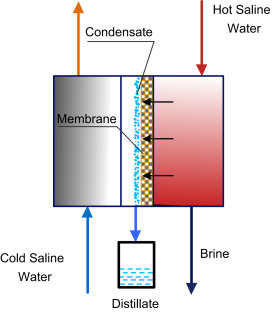
\includegraphics[width=0.8\linewidth]{Imagens/chap01/membrane.png}
    \caption[Representação esquemática do processo de dessalinização]{Representação esquemática do processo de dessalinização, no qual a água salina é submetida a um processo de separação para obtenção de água dessalinizada e de uma corrente concentrada em sais. Fonte: ...}
    \label{fig:processo_dessalinizacao}
\end{figure}

As tecnologias baseadas em membrana incluem a osmose reversa (do inglês, \textit{Reverse Osmosis} -- RO), nanofiltração (do inglês, \textit{Nanofiltration} -- NF), osmose direta (do inglês, \textit{Forward Osmosis} -- FO) e eletrodiálise (do inglês, \textit{Electrodialysis} -- ED). A RO, amplamente utilizada, emprega alta pressão para forçar a passagem de água por uma membrana semipermeável, enquanto a FO utiliza gradientes osmóticos e a ED campos elétricos para separação iônica. Alternativamente, a dessalinização por congelamento (do inglês, \textit{Freeze Desalination} -- FD) promove a separação da água na forma de cristais de gelo. A escolha da tecnologia depende de fatores como qualidade da água de alimentação, demanda energética e custos operacionais (\cite{Abid2020DesalinationOverview}).

Nesse contexto, a destilação por membrana (do inglês, \textit{Membrane Distillation} -- MD) destaca-se como um processo híbrido que combina princípios térmicos e de separação por membranas. A MD baseia-se na migração de vapor de água através de uma membrana hidrofóbica, impulsionada por uma diferença de pressão de vapor induzida por gradiente de temperatura, resultando em elevada rejeição de sais (\cite{Abid2020DesalinationOverview,Cath2010}).

A MD apresenta vantagens como operação em condições moderadas de temperatura e pressão, possibilidade de uso de fontes térmicas de baixa qualidade ou calor residual, e aplicabilidade em soluções de alta salinidade. Exemplos dessas fontes incluem sistemas de dessalinização alimentados por energia solar térmica, unidades integradas a calor residual proveniente de processos industriais, usinas de energia e sistemas marítimos, bem como o uso de energia geotérmica e configurações híbridas com recuperação de calor. Estudos também reportam o desenvolvimento de unidades piloto de MD alimentadas por energia solar, evidenciando a viabilidade técnica e econômica dessas integrações (\cite{Yadav2021MDLowGradeEnergy}). Além disso, avanços recentes, como integração com fontes renováveis, recuperação de calor latente e desenvolvimento de módulos escaláveis, têm reforçado seu potencial para aplicações em larga escala, destacando a importância da modelagem para o projeto e otimização desses sistemas (\cite{Cath2010,Leaper2021,Warsinger2017,Parani2021,AndresManas2022}).

Diferentes configurações de MD foram desenvolvidas, distinguindo-se principalmente pelos mecanismos de transporte de vapor e pelas estratégias de condensação/coleta do permeado. Entre as principais configurações, destacam-se a destilação por membrana de contato direto (do inglês, \textit{Direct Contact Membrane Distillation} -- DCMD), na qual o vapor gerado na alimentação quente atravessa a membrana e condensa diretamente em uma corrente fria em contato com o permeado; a destilação por membrana com gás de varredura (do inglês, \textit{Sweeping Gas Membrane Distillation} -- SGMD), em que um gás de arraste remove o vapor do lado do permeado e o conduz a um condensador externo; e a destilação por membrana a vácuo (do inglês, \textit{Vacuum Membrane Distillation} -- VMD), na qual a aplicação de vácuo parcial no lado do permeado intensifica o transporte de vapor, sendo este posteriormente condensado fora do módulo.

A configuração de destilação por membrana com lacuna de ar (do inglês, \textit{Air Gap Membrane Distillation} -- AGMD) se destaca pela presença de uma camada de ar entre a membrana e a superfície de condensação, que reduz perdas térmicas por condução, mas introduz resistência ao transporte de massa. Essa resistência adicional aumenta o caminho difusivo do vapor e, consequentemente, reduz o fluxo de permeado em comparação a outras configurações, como DCMD e VMD, evidenciando um compromisso entre eficiência térmica e taxa de produção de água dessalinizada (\cite{AlZoubi2018,Chong2022,Abid2020DesalinationOverview}).

Uma evolução dessa configuração é a destilação por membrana com lacuna de ar aprimorada por vácuo (do inglês, \textit{Vacuum-Enhanced Air Gap Membrane Distillation} -- V-AGMD), na qual a aplicação de pressão reduzida no espaço de ar diminui a resistência ao transporte de vapor, aumentando o fluxo de permeado, ao mesmo tempo em que mantém o isolamento térmico proporcionado pela presença da camada de ar. Essa configuração apresenta potencial promissor, especialmente quando associada a fontes de calor de baixa qualidade (\cite{Warsinger2017,Zewdie2020}).

O desempenho de sistemas V-AGMD depende fortemente de variáveis operacionais, como as temperaturas de entrada das correntes de alimentação e de resfriamento, a salinidade da alimentação, as vazões e a pressão no espaço de ar. No processo MD, os fenômenos de transferência de calor e massa ocorrem de forma simultânea e acoplada: o gradiente térmico determina a diferença de pressão de vapor que impulsiona o transporte de massa, enquanto a evaporação e a condensação alteram os fluxos de calor no módulo. Além disso, a salinidade, a vazão e o nível de vácuo afetam as resistências ao transporte e a força motriz do processo. Dessa forma, a resposta do sistema resulta da interação entre múltiplas variáveis operacionais, tornando desafiadora a previsão simultânea do fluxo de permeado e das temperaturas de saída das correntes de alimentação e de resfriamento. A estimativa adequada dessas temperaturas é particularmente relevante, pois elas podem ser utilizadas no cálculo de indicadores de desempenho energético, como o consumo específico de energia (SEC) e o ganho de saída (GOR) (\cite{Hitsov2015,Olatunji2018}).

De modo geral, a modelagem de sistemas de destilação por membranas pode seguir duas abordagens principais: modelos físico-matemáticos e modelos baseados em dados experimentais. Os modelos físico-matemáticos representam o processo a partir de balanços de massa e energia, relações termodinâmicas e mecanismos de transferência de calor e massa. Por isso, apresentam elevada interpretabilidade física e consistência termodinâmica, embora frequentemente exijam simplificações estruturais ou elevado esforço computacional (\cite{Hitsov2015,Olatunji2018}). Por outro lado, os modelos baseados em dados experimentais utilizam medições do sistema para aprender relações entre variáveis operacionais e variáveis de desempenho, por meio de técnicas como regressão e redes neurais artificiais. Esses modelos podem capturar relações complexas sem exigir a formulação explícita de todos os fenômenos envolvidos, mas dependem fortemente da disponibilidade, representatividade e qualidade dos dados experimentais utilizados no treinamento (\cite{Zhu2022}).

Para os modelos baseados em dados experimentais, a obtenção de observações em sistemas reais é frequentemente limitada e onerosa, o que torna a capacidade de generalização um desafio central. Nesse contexto, modelos de maior complexidade, isto é, modelos com maior capacidade de adaptação aos dados de treinamento, podem apresentar bom desempenho durante o ajuste, mas falhar quando aplicados a novas condições operacionais. Essa complexidade pode estar associada, por exemplo, ao número de parâmetros do modelo, à profundidade de árvores, à quantidade de camadas ou neurônios em redes neurais e ao grau de regularização adotado. Além disso, a avaliação baseada apenas em métricas médias pode mascarar instabilidades associadas à variabilidade dos dados e das partições de validação, tornando essencial a adoção de estratégias robustas de validação (\cite{Vabalas2019,Yip2019,Roberts2017,Kirk2024}).

Diante dessas limitações, abordagens híbridas de modelagem têm emergido como uma alternativa promissora, combinando modelos físico-matemáticos com técnicas baseadas em dados. A incorporação de conhecimento físico no processo de aprendizado pode restringir o espaço de soluções admissíveis, reduzir a dependência de grandes volumes de dados e melhorar a capacidade de generalização dos modelos (\cite{Xu2022,Muther2022,Kasilingam2024}).

Nesse contexto, torna-se necessária a adoção de uma abordagem metodológica estruturada para a avaliação e seleção de modelos de regressão supervisionada aplicados ao processo V-AGMD, considerando simultaneamente a natureza não linear do sistema, as limitações do conjunto de dados disponível e o potencial de integração entre conhecimento físico e aprendizado baseado em dados.

\section{Motivação}

O presente trabalho está inserido no contexto das atividades desenvolvidas no Laboratório de Micro e Nanofluídica e Microssistemas (LabMEMS) da Universidade Federal do Rio de Janeiro (UFRJ), no âmbito de um projeto multidisciplinar voltado à cogeração sustentável de energia elétrica e produção de água potável a partir do aproveitamento de energia solar térmica. Nesse sistema, painéis solares são utilizados para aquecer a corrente de alimentação de uma unidade piloto de destilação por membranas, disponível comercialmente, com capacidade de operação nas configurações AGMD e V-AGMD, permitindo integrar geração de energia e dessalinização em uma mesma planta experimental.

A motivação deste estudo decorre da necessidade de compreender e prever o desempenho dessa planta de cogeração, especialmente no módulo de dessalinização por membranas operado na configuração V-AGMD, na qual há presença de espaço de ar e aplicação de vácuo parcial. O sistema experimental fornece dados reais obtidos sob diferentes regimes operacionais, nos quais variáveis como temperaturas de entrada, vazões, salinidade e nível de vácuo parcial influenciam simultaneamente o fluxo de permeado e as temperaturas de saída das correntes. A previsão dessas grandezas é relevante tanto para avaliar a produção de água dessalinizada quanto para estimar indicadores energéticos associados ao processo.

Além dos dados experimentais, foi utilizado como referência comparativa um modelo físico-matemático reduzido do tipo 0D, previamente descrito na literatura para esse sistema (\cite{Lisboa2024}). A disponibilidade simultânea de dados reais da planta de cogeração e de um modelo físico reduzido permite investigar estratégias de modelagem baseadas em dados e abordagens híbridas, nas quais informações provenientes da física do processo podem complementar o aprendizado dos modelos.

Dessa forma, a motivação central deste trabalho está na necessidade de avaliar ferramentas preditivas capazes de representar o desempenho de sistemas V-AGMD a partir de dados experimentais limitados, explorando simultaneamente o potencial de modelos baseados em dados e de estratégias híbridas que incorporam conhecimento físico. Assim, o estudo busca contribuir para a análise, operação e futura otimização de sistemas V-AGMD integrados a fontes renováveis de energia.

\section{Objetivos}

\subsection{Objetivo geral}

O objetivo geral deste trabalho é avaliar estratégias de modelagem baseada em dados e modelagem híbrida físico--dados para a predição do desempenho de um sistema de destilação por membranas do tipo V-AGMD, considerando como variáveis de saída o fluxo de permeado e as temperaturas de saída das correntes de alimentação e resfriamento.

\subsection{Objetivos específicos}

Para atingir o objetivo geral, são definidos os seguintes objetivos específicos:

\begin{itemize}
    \item estruturar a base de dados experimental do sistema V-AGMD, definindo variáveis de entrada, variáveis de saída e agrupamentos por regime operacional;

    \item avaliar o desempenho de um modelo físico reduzido 0D como referência comparativa para as variáveis de saída do sistema;

    \item comparar diferentes famílias de modelos de regressão supervisionada, incluindo modelos lineares, modelos baseados em árvores, redes neurais artificiais e arquiteturas híbridas;

    \item aplicar uma estratégia de validação cruzada por grupos, considerando a separação entre regimes experimentais, de modo a avaliar a capacidade de generalização dos modelos;

    \item selecionar o modelo final com base em critérios de desempenho preditivo, diferença de generalização e complexidade estrutural;

    \item analisar o potencial da incorporação de informações físicas na melhoria do desempenho de modelos baseados em dados para a predição do processo V-AGMD.
\end{itemize}

\section{Organização do TCC}

Este trabalho está organizado em seis capítulos. O Capítulo 1 apresenta a introdução, incluindo a contextualização do problema, a motivação do estudo, os objetivos e a organização do documento.

O Capítulo 2 apresenta a revisão bibliográfica sobre a modelagem de sistemas de destilação por membranas, abordando modelos baseados em primeiros princípios, modelos orientados por dados, estratégias híbridas e lacunas da literatura.

O Capítulo 3 reúne a fundamentação teórica necessária ao trabalho, incluindo os princípios da destilação por membranas, o modelo físico reduzido utilizado como referência e os conceitos de aprendizado de máquinas aplicados à regressão.

O Capítulo 4 descreve a metodologia proposta, contemplando a preparação dos dados, a validação cruzada, os critérios de seleção, as famílias de modelos avaliadas e as estratégias de integração com o modelo físico.

O Capítulo 5 apresenta os resultados, incluindo a análise exploratória dos dados, a avaliação do modelo físico reduzido, a comparação entre modelos baseados em dados e a seleção do modelo final.

Por fim, o Capítulo 6 apresenta as conclusões do trabalho e sugestões para pesquisas futuras.
    \chapter{Revisão Bibliográfica}
\label{chap3}

Este capítulo apresenta a revisão bibliográfica que fundamenta a análise desenvolvida neste trabalho, com foco nas abordagens de modelagem aplicadas a sistemas de destilação por membranas. Inicialmente, são retomados aspectos gerais do processo de destilação por membranas, de modo a situar o leitor quanto aos fenômenos físicos envolvidos e às variáveis de desempenho de interesse. Em seguida, são discutidas as principais estratégias de modelagem adotadas na literatura, incluindo modelos baseados em primeiros princípios, modelos orientados por dados e abordagens híbridas, destacando suas vantagens, limitações e contribuições para o estudo de sistemas de MD. A partir dessa análise, são identificadas lacunas que justificam a proposta metodológica adotada neste estudo.

% CITAÇÃO NECESSÁRIA: Incluir uma referência geral para a definição e os princípios da destilação por membranas, caso as referências ExperimentalMD e S2MD não sejam suficientes para sustentar este parágrafo.
A destilação por membranas é um processo de separação térmico baseado no transporte de vapor através de uma membrana hidrofóbica e microporosa. A força motriz do processo é a diferença de pressão parcial de vapor entre os dois lados da membrana, geralmente estabelecida por uma diferença de temperatura entre as correntes. Nesse processo, a fase líquida é impedida de atravessar os poros da membrana, enquanto o vapor de água migra para o lado de menor pressão parcial, onde é posteriormente condensado.

\section{Modelagem de Sistemas de Destilação por Membranas}
\label{sec:modelagem_md}

A modelagem matemática de sistemas de destilação por membranas é estudada porque permite descrever, prever e analisar o desempenho do processo sem depender exclusivamente de campanhas experimentais extensas. Em sistemas de MD, essa previsão é particularmente relevante porque o desempenho do processo envolve tanto a produtividade, associada ao fluxo de permeado, quanto parâmetros de eficiência energética, que dependem das temperaturas de saída das correntes quente e fria. Essas variáveis são determinadas por fenômenos simultâneos de transferência de calor e massa, evaporação na interface quente, transporte de vapor através da membrana e condensação no lado frio (\cite{ExperimentalMD, S2MD}). Assim, modelos matemáticos são ferramentas importantes tanto para a compreensão dos mecanismos dominantes quanto para o projeto, otimização e ampliação de escala desses sistemas.

Entretanto, a modelagem desses sistemas permanece desafiadora devido ao caráter acoplado e não linear dos fenômenos envolvidos. A resposta do processo depende de variáveis operacionais como temperatura de alimentação, temperatura de resfriamento, vazões, pressão de vácuo e salinidade, além de propriedades da membrana e de efeitos como polarização térmica, perdas de calor, resistência ao transporte de massa e possíveis não idealidades experimentais. Esses desafios tornam-se ainda mais relevantes quando se passa de sistemas em escala de bancada para unidades em escala piloto, nas quais efeitos associados à geometria do módulo, distribuição de escoamento, instrumentação, perdas térmicas e variações operacionais podem reduzir a aderência de modelos simplificados às medições experimentais (\cite{Lisboa2024}).

% CITAÇÃO NECESSÁRIA: Verificar se ReviewAI_MD sustenta diretamente esta classificação em três categorias. Caso contrário, incluir uma referência adicional de revisão sobre modelagem em MD ou sobre modelagem físico-matemática, orientada por dados e híbrida.
De modo geral, as abordagens de modelagem aplicadas à destilação por membranas podem ser classificadas em três categorias principais: modelos baseados em primeiros princípios, modelos orientados por dados e abordagens híbridas (\cite{ReviewAI_MD}).

\subsection{Abordagens de modelagem física em destilação por membranas}

A modelagem física de sistemas de destilação por membranas pode ser desenvolvida com diferentes níveis de detalhamento, dependendo do objetivo do estudo, da configuração analisada e do custo computacional admissível. Em geral, essas abordagens buscam descrever os mecanismos acoplados de transferência de calor e massa que governam o processo, incluindo evaporação na interface quente, transporte de vapor através da membrana, difusão no domínio gasoso e condensação na região fria. Dessa forma, diferenciam-se de modelos puramente empíricos por partirem de leis físicas fundamentais, como balanços de massa e energia, equações de transporte e relações fenomenológicas associadas ao processo.

No contexto da destilação por membranas, uma primeira forma de modelagem física consiste na formulação de modelos distribuídos ou semi-distribuídos, capazes de representar variações espaciais das variáveis do processo. Esses modelos podem descrever gradientes de temperatura, concentração, pressão ou velocidade ao longo do módulo, permitindo uma análise mais detalhada dos fenômenos de transporte. No entanto, esse maior nível de detalhamento normalmente exige maior número de parâmetros, propriedades físicas, correlações de transporte e condições de contorno bem definidas.

Um exemplo dessa abordagem é o trabalho de \cite{Alsaadi2013}, que desenvolve um modelo unidimensional para módulos planos de AGMD. Nesse modelo, o módulo é discretizado ao longo da direção do escoamento e são consideradas as principais regiões do sistema: canal de alimentação aquecido, membrana polimérica, espaço de ar, filme de condensado, placa de resfriamento e canal frio. A formulação permite acompanhar a variação longitudinal das condições de operação e foi validada experimentalmente para avaliar o comportamento do processo em escoamentos co-corrente e contracorrente.

No modelo de \cite{Alsaadi2013}, são adotadas hipóteses como regime permanente, escoamento unidimensional, ausência de perdas de calor para o ambiente, pressão constante no espaço de ar e transporte de massa no espaço de ar predominantemente por difusão. O transporte de vapor através da membrana é representado pela combinação entre difusão molecular e difusão de Knudsen, enquanto a transferência de calor é descrita por mecanismos de convecção nos canais, condução através da membrana e do espaço de ar, e liberação de calor latente durante a condensação. Assim, o estudo exemplifica uma modelagem física mais detalhada, capaz de representar a distribuição longitudinal dos fenômenos de transporte, mas ainda baseada em hipóteses simplificadoras para manter o problema tratável.

Modelos físicos ainda mais detalhados podem ser formulados com base em abordagens bidimensionais e ferramentas de dinâmica dos fluidos computacional. Nesse sentido, \cite{Ansari2022} propõem um modelo bidimensional para AGMD em módulo plano contracorrente, com o objetivo de capturar a variação do fluxo de água ao longo do comprimento do módulo e comparar o desempenho da configuração AGMD com a DCMD. A formulação considera o canal de alimentação, a membrana hidrofóbica, o espaço de ar, o filme de condensado, a placa de resfriamento e o canal de permeado, sendo acoplada à solução das equações de continuidade, quantidade de movimento e energia por meio de CFD.

Essa abordagem permite representar de forma mais detalhada as variações espaciais do processo, sendo útil para investigar efeitos locais e limitações de desempenho que não seriam capturados por modelos concentrados. Por outro lado, a maior fidelidade física implica aumento da complexidade matemática e da demanda computacional, além de maior dependência de propriedades, correlações e condições de contorno. Assim, modelos distribuídos são particularmente úteis para análises mecanísticas detalhadas, mas podem ser menos práticos quando o objetivo é obter estimativas rápidas de desempenho ou integrar a modelagem física a rotinas de otimização e aprendizado de máquina.

Nesse contexto, modelos físicos reduzidos surgem como uma alternativa para representar o comportamento global do sistema com menor custo computacional. Diferentemente das formulações distribuídas ou bidimensionais, esses modelos utilizam grandezas médias ou efetivas, balanços globais e resistências equivalentes para estimar variáveis de desempenho. O modelo proposto por \cite{Lisboa2024}, por exemplo, representa uma formulação reduzida para um sistema V-AGMD em escala piloto, permitindo estimar grandezas como fluxo de permeado e temperaturas de saída sem resolver explicitamente os perfis espaciais ao longo do módulo.

A principal vantagem dos modelos reduzidos está na simplicidade de implementação e no menor custo de simulação, o que favorece sua utilização como referência física em pipelines de modelagem preditiva. Entretanto, essa simplificação também limita a representação de fenômenos locais, como gradientes axiais de temperatura, concentração e velocidade, efeitos hidrodinâmicos, perdas térmicas distribuídas e não idealidades geométricas do módulo. Dessa forma, modelos reduzidos apresentam um compromisso entre coerência física, baixo custo computacional e menor detalhamento fenomenológico.

A literatura mostra, portanto, que a modelagem física em destilação por membranas pode variar desde formulações unidimensionais ou bidimensionais, voltadas à descrição detalhada dos mecanismos de transporte, até modelos reduzidos de parâmetros concentrados, voltados à estimativa global do desempenho. Essa diversidade evidencia um compromisso entre fidelidade física, custo computacional, disponibilidade de parâmetros e aplicabilidade prática. No presente trabalho, esse panorama é relevante porque o modelo físico reduzido de \cite{Lisboa2024} é utilizado não como uma descrição completa do sistema, mas como uma referência físico-matemática simplificada, posteriormente incorporada à análise comparativa com modelos orientados por dados e abordagens híbridas.
\subsection{Modelos orientados por dados}

Modelos orientados por dados, também conhecidos como modelos \textit{data-driven}, surgem como uma alternativa atrativa quando se busca reduzir o custo computacional associado à simulação detalhada de sistemas de destilação por membranas. Em vez de resolver explicitamente as equações físicas do processo, esses modelos aprendem relações entre variáveis operacionais e saídas de interesse a partir de dados experimentais ou simulados, permitindo obter respostas rápidas após a etapa de treinamento.

% CITAÇÃO NECESSÁRIA: Inserir aqui trabalhos de MD que utilizaram planejamento experimental, regressão estatística ou metodologia de superfície de resposta, especialmente em unidades de bancada ou piloto.
Além das redes neurais artificiais, a literatura de MD também apresenta estudos baseados em planejamento experimental, regressão e metodologia de superfície de resposta. Nesses trabalhos, conjuntos planejados de experimentos são utilizados para ajustar equações empíricas capazes de relacionar variáveis operacionais, como temperatura, vazão, salinidade e pressão, a respostas do processo, como fluxo de permeado, rejeição de sais e indicadores de desempenho. Essas abordagens funcionam como metamodelos úteis para análise de sensibilidade e otimização local, especialmente em sistemas de bancada e unidades piloto.

% CITAÇÃO NECESSÁRIA: Verificar com a professora o trabalho/dissertação do Francisco, aluno da professora Carolina, que utilizou abordagem semelhante. Após localizar a referência, inserir aqui a contribuição específica do estudo.
No entanto, por serem ajustados a partir de um conjunto específico de dados, modelos empíricos baseados em planejamento experimental e regressão tendem a ser mais confiáveis dentro da faixa experimental considerada. Assim, embora sejam úteis para interpretação estatística dos efeitos operacionais e para otimização local, sua extrapolação para condições distintas daquelas utilizadas no ajuste deve ser realizada com cautela.

Na destilação por membranas, modelos orientados por dados também têm sido amplamente empregados na previsão do desempenho do processo por meio de redes neurais artificiais. Essas redes são utilizadas para mapear diretamente variáveis operacionais em saídas de interesse, como fluxo de permeado e temperaturas de saída (\cite{ANN_AGMD, ANN_VMD_Fouling}).

Esses modelos apresentam alta capacidade de aproximação de funções não lineares e bom desempenho dentro da faixa de treinamento. Contudo, sua generalização é limitada e dependente da distribuição dos dados (\cite{ReviewAI_MD}), podendo gerar previsões inconsistentes fora dessa região.

Dessa forma, embora os modelos orientados por dados apresentem potencial para representar relações não lineares em sistemas de MD, sua aplicação exige atenção à representatividade dos dados e à estratégia de validação adotada. Essa questão é particularmente relevante em sistemas experimentais organizados em regimes operacionais distintos, nos quais divisões aleatórias podem superestimar a capacidade de generalização do modelo.

\subsection{Abordagens híbridas}

Embora menos frequentes do que os modelos puramente físicos ou puramente orientados por dados, algumas abordagens buscam combinar conhecimento físico e aprendizado a partir de dados. Neste trabalho, essas estratégias são tratadas como abordagens híbridas, pois associam, em diferentes níveis, a coerência física dos modelos baseados em primeiros princípios à flexibilidade dos modelos ajustados a partir de dados experimentais ou simulados.

De modo geral, essas abordagens podem ser construídas de diferentes formas. Uma possibilidade consiste em incorporar equações físicas, balanços ou restrições do processo diretamente à formulação do modelo ou à função de perda. Outra possibilidade é utilizar um modelo físico como estimativa inicial e empregar um modelo orientado por dados para corrigir seus desvios em relação aos dados experimentais. Dessa forma, a informação física pode atuar tanto como elemento de regularização quanto como referência para o aprendizado de correções.

No contexto da destilação por membranas, uma das estratégias encontradas corresponde às \textit{Physics-Informed Neural Networks} (PINNs), nas quais as equações governantes são incorporadas à função de perda. O trabalho de \cite{PINN_MD}, por exemplo, utiliza esse tipo de abordagem para incluir conhecimento físico no treinamento da rede neural, buscando melhorar a consistência das previsões em relação aos fenômenos que regem o processo.

Outra classe de abordagem envolve modelos residuais, nos quais um modelo físico fornece uma estimativa inicial e uma rede neural é treinada para aprender a diferença entre essa estimativa e os dados experimentais. Essa estratégia é explorada em trabalhos como \cite{Zhou2024, zheng2021knowledge}, que destacam a possibilidade de combinar previsões baseadas em conhecimento físico com correções aprendidas a partir dos dados.

% CITAÇÃO NECESSÁRIA: Caso o trabalho do Francisco tenha utilizado abordagem híbrida, inserir aqui a referência e explicar a contribuição específica. Caso tenha utilizado planejamento experimental ou regressão, manter a referência na subseção de modelos orientados por dados.
As abordagens híbridas se inserem, portanto, como uma alternativa para combinar as vantagens dos modelos físicos e dos modelos orientados por dados. Sua principal contribuição está na tentativa de preservar coerência física sem abrir mão da capacidade preditiva dos métodos ajustados por dados, o que é particularmente relevante em sistemas experimentais complexos, com dados limitados ou sujeitos a não idealidades não completamente representadas por modelos simplificados.

\subsection{Síntese e lacunas}

A partir da literatura analisada, observa-se que a modelagem de sistemas de destilação por membranas tem sido conduzida por diferentes estratégias. Modelos baseados em primeiros princípios contribuem para a compreensão mecanística do processo e para a análise de condições operacionais não exploradas experimentalmente. Modelos empíricos, baseados em planejamento experimental e regressão, permitem construir metamodelos úteis para análise de sensibilidade e otimização local. Já os modelos orientados por dados, especialmente redes neurais artificiais, ampliam a capacidade de representar relações não lineares entre variáveis operacionais e respostas do processo. Por fim, as abordagens híbridas buscam combinar coerência física e capacidade preditiva, utilizando o conhecimento físico como restrição, referência ou ponto de partida para modelos ajustados a partir de dados.

Apesar desses avanços, a literatura ainda apresenta limitações metodológicas relevantes. Predomina o uso de divisões simples dos dados, como 70/15/15 ou 80/20, geralmente realizadas de forma aleatória (\cite{ANN_VMD_Fouling, ReviewAI_MD}). Essa prática desconsidera a estrutura dos dados experimentais, como regimes operacionais distintos e dependências entre amostras.

Além disso, raramente são utilizadas estratégias mais robustas de validação, como validação cruzada, sendo comum a avaliação baseada em uma única divisão dos dados (\cite{ANN_VMD_Fouling}), o que pode introduzir viés. Essa limitação é particularmente importante em sistemas experimentais nos quais diferentes amostras podem estar associadas a um mesmo regime operacional ou a condições próximas de operação.

A seleção de modelos e hiperparâmetros é frequentemente realizada de forma heurística, com otimização limitada e baseada apenas na minimização de métricas como RMSE ou MSE, sem consideração explícita de complexidade ou variabilidade estatística (\cite{ANN_VMD_Fouling}). Adicionalmente, a maioria dos estudos avalia os modelos apenas em regime de interpolação, com pouca análise da capacidade de extrapolação (\cite{ANN_VMD_Fouling, ReviewAI_MD}).

Alguns trabalhos, contudo, adotam abordagens mais robustas. O estudo de \cite{PINN_MD} utiliza validação cruzada e avalia cenários futuros, enquanto \cite{ANN_AGMD} emprega validação externa independente. Já \cite{Zhou2024} apresenta uma abordagem híbrida com busca sistemática de hiperparâmetros e análise explícita de generalização.

Dessa forma, evidencia-se uma lacuna na adoção de estratégias de validação mais rigorosas, na consideração da estrutura dos dados experimentais e na análise da capacidade de generalização dos modelos em sistemas reais. Nesse contexto, este trabalho contribui ao investigar modelos orientados por dados e abordagens híbridas aplicados a um sistema V-AGMD em escala piloto, incorporando informação física proveniente de um modelo reduzido e adotando uma estratégia de validação compatível com a organização dos dados experimentais.    
    \chapter{Fundamentação Teórica}

Este capítulo apresenta os fundamentos teóricos que embasam este trabalho, abrangendo tanto os aspectos físicos associados ao processo de destilação por membranas quanto os conceitos de aprendizado de máquinas utilizados na modelagem baseada em dados. Inicialmente, são discutidos os princípios de funcionamento da destilação por membranas e os mecanismos de transporte de massa e calor que governam o processo, bem como a formulação de modelos físicos reduzidos. Em seguida, são apresentados os principais conceitos de aprendizado supervisionado, incluindo formulação de problemas de regressão, métricas de avaliação, estratégias de validação e controle de complexidade. Por fim, são descritas as principais famílias de modelos utilizadas, assim como abordagens híbridas que integram conhecimento físico e aprendizado de máquina, estabelecendo a base conceitual para a metodologia adotada neste trabalho.



\section{Destilação por Membranas}

\subsection{Princípios Físicos}

Conforme discutido anteriormente, a destilação por membranas é baseada na migração de vapor de água através de uma membrana hidrofóbica, impulsionada por uma diferença de pressão parcial de vapor entre a solução salina aquecida e uma região fria. Nesta seção, retomam-se apenas os princípios físicos relevantes para a compreensão do processo e das variáveis utilizadas na modelagem desenvolvida neste trabalho. A força motriz do processo decorre do gradiente térmico estabelecido entre a alimentação aquecida e uma região de menor temperatura, o que gera uma diferença de pressão de vapor ao longo da membrana. A membrana atua como uma barreira não molhável ao escoamento do líquido, permitindo apenas a passagem do vapor d'água. O mecanismo fundamental envolve evaporação na interface do lado quente, transporte do vapor através dos poros da membrana e posterior remoção ou condensação do vapor, dependendo da configuração de MD considerada (\cite{Cath2010, Hitsov2015}).

A força motriz do processo decorre do gradiente térmico estabelecido entre a corrente quente de alimentação e a corrente fria de condensação, o que gera uma diferença de pressão de vapor ao longo da membrana. A membrana atua como uma barreira não molhável ao escoamento do líquido, permitindo apenas a passagem da fase vapor. O mecanismo fundamental envolve evaporação na interface do lado quente, difusão do vapor através dos poros da membrana e posterior condensação no lado frio (\cite{Cath2010, Hitsov2015}).

Diversas configurações de MD são descritas na literatura, diferenciando-se principalmente pela forma como o vapor é removido e condensado após atravessar a membrana (\cite{Cath2010, Warsinger2017, AlZoubi2018, Chong2022}). As quatro configurações básicas mais recorrentes são:

\begin{itemize}
    \item \textit{Direct Contact Membrane Distillation} (DCMD): as correntes quente e fria entram em contato direto com os lados opostos da membrana. Apresenta construção simples e condensação interna do vapor, mas pode sofrer maiores perdas térmicas por condução através da membrana.

    \item \textit{Air Gap Membrane Distillation} (AGMD): há um espaço de ar de ar entre a membrana e a superfície de condensação. Essa configuração reduz perdas térmicas por condução e permite a condensação interna do permeado, mas o espaço de ar adiciona resistência ao transporte de massa, podendo reduzir o fluxo de permeado.

    \item \textit{Vacuum Membrane Distillation} (VMD): aplica-se vácuo no lado do permeado, removendo o ar e reduzindo a resistência difusiva ao transporte de vapor. Embora possa favorecer maiores fluxos de permeado, essa configuração exige condensação externa do vapor produzido, aumentando a complexidade do sistema.

    \item \textit{Sweeping Gas Membrane Distillation} (SGMD): utiliza-se um gás de arraste no lado do permeado para remover o vapor que atravessa a membrana. Essa configuração reduz a pressão parcial de vapor no lado do permeado, mas também requer condensação externa e controle adicional do escoamento do gás.
\end{itemize}

Além dessas configurações básicas, existem arranjos derivados que combinam características de mais de uma configuração. Entre eles, destaca-se a \textit{Vacuum-Enhanced Air Gap Membrane Distillation} (V-AGMD), adotada neste trabalho, que combina o espaço de ar de ar característico da AGMD com operação sob pressão reduzida. Essa configuração busca reduzir a resistência ao transporte de massa, mantendo a condensação interna no módulo, o que pode favorecer o desempenho do sistema sem exigir condensação externa do permeado (\cite{Lisboa2024}).

% CITAÇÃO NECESSÁRIA: Verificar se Lisboa2024 ou outra referência específica sustenta diretamente a descrição da configuração V-AGMD e suas vantagens operacionais.
% FIGURA OPCIONAL: Inserir figura esquemática comparando DCMD, AGMD, VMD e SGMD, caso haja uma fonte adequada ou figura autoral.

A escolha da configuração influencia diretamente os mecanismos dominantes de transferência de massa e calor e, consequentemente, o desempenho térmico e energético do sistema \cite{Warsinger2017,Hitsov2015}.
\subsection{Modelagem do Transporte de Massa}

Como este trabalho trata de um sistema V-AGMD, a descrição do transporte de massa é direcionada às configurações AGMD e V-AGMD. Nessas configurações, o vapor formado na interface entre a solução salina aquecida e a membrana atravessa os poros da membrana e, em seguida, percorre uma região gasosa até a superfície de condensação. No caso da V-AGMD, esse transporte ocorre sob pressão reduzida, o que altera a resistência difusiva associada à presença de ar no domínio gasoso.

O transporte de vapor através da membrana pode ser descrito pelo modelo de \textit{Dusty Gas}, uma formulação que contempla diferentes contribuições ao transporte em meios porosos, incluindo difusão molecular, difusão de Knudsen, difusão superficial e escoamento viscoso ou convectivo nos poros. No entanto, a depender das condições do sistema e das hipóteses simplificadoras adotadas, algumas dessas contribuições podem ser desconsideradas. No modelo utilizado como referência neste trabalho, considera-se a combinação entre difusão molecular e difusão de Knudsen, enquanto efeitos associados à difusão superficial e ao escoamento viscoso do tipo Poiseuille são negligenciados (\cite{Lisboa2024}).

\begin{figure}[H]
    \centering
    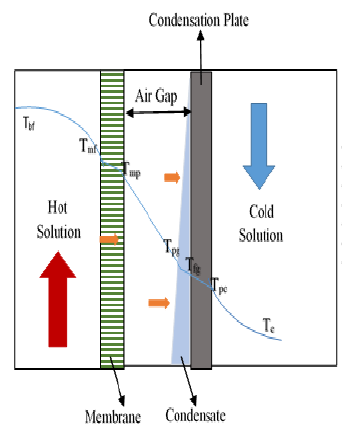
\includegraphics[width=0.5\linewidth]{Imagens/chap03/Model-of-heat-and-mass-transfer-in-the-AGMD.png}
    \caption[Domínio considerado na modelagem do transporte de massa em AGMD/V-AGMD]{Representação esquemática do domínio considerado na modelagem do transporte de massa em configurações AGMD e V-AGMD, incluindo a interface de evaporação, os poros da membrana, o espaço de ar gasoso e a superfície de condensação.}
    \fonte{Autor: \cite{Zheng2017}}
    \label{fig:dominio_transporte_agmd_vagmd}
\end{figure}

A formulação geral pode ser escrita como

\begin{equation}
\frac{N_w}{D_w^k} + \frac{p_a N_w - p_w N_a}{D_{wa}^0}
=
-\frac{1}{R T_m}\frac{d p_w}{dx}
\end{equation}

\noindent em que \(N_w\) é o fluxo molar de vapor de água, \(D_w^{K}\) é a difusividade de Knudsen, \(D_w^{M}\) é a difusividade molecular do vapor de água no ar, \(p_w\) e \(P\) são, respectivamente, a pressão parcial do vapor de água e a pressão total do sistema, \(R\) é a constante universal dos gases e \(T_m\) é a temperatura média na membrana.

Assumindo ausência de fluxo molar de ar \((N_a \approx 0)\), a expressão pode ser simplificada e, após integração ao longo da espessura da membrana \(\delta_m\), obtém-se uma forma funcional para o fluxo mássico de permeado \(j_w\):

\begin{equation}
j_w = \frac{M_w D_{wa}^{0}}{R T_m \delta_m}
\ln \left(
\frac{D_{wa}^{0} - D_{\mathrm{eff}} p_{mg}}
{D_{wa}^{0} - D_{\mathrm{eff}} p_{mf}}
\right)
\end{equation}

\noindent em que \(M_w\) é a massa molar da água, \(p_{mf}\) é a pressão parcial de vapor na interface entre a solução salina aquecida e a membrana, e \(p_{mg}\) é a pressão parcial de vapor junto à superfície fria de condensação, localizada após o espaço de ar gasoso. Nas configurações AGMD e V-AGMD, essa superfície corresponde à região onde se forma o filme de água condensada. Dessa forma, a diferença de temperatura entre a interface da solução salina aquecida e a superfície de condensação estabelece o gradiente de pressão parcial responsável pela evaporação e pelo transporte de vapor através da membrana e do espaço de ar.

Para pequenas diferenças de pressão parcial, a expressão pode ser linearizada como

\begin{equation}
j_w = B_m (p_{mf} - p_{mg})
\end{equation}

em que $B_m$ representa o coeficiente global de transferência de massa da membrana.

No espaço de ar, o transporte difusivo pode ser descrito por

\begin{equation}
j_w = B_g (p_{mg} - p_{gl})
\end{equation}

onde $B_g$ é o coeficiente de transferência de massa no air gap e $p_{gl}$ é a pressão parcial de vapor na interface do condensador. Considerando resistências difusivas em série:

\begin{equation}
\frac{1}{B_{eq}} = \frac{1}{B_m} + \frac{1}{B_g}
\end{equation}

resultando em

\begin{equation}
j_w = B_{eq} (p_{mf} - p_{gl})
\end{equation}

A presença de sal na alimentação reduz a pressão de vapor da água. Esse efeito é frequentemente incorporado por meio da atividade da água $a_w$, de forma que

\begin{equation}
p_{mf} = a_w (1 - x_{salt}) p_v
\end{equation}

onde $x_{salt}$ é a fração molar de sal e $p_v$ é a pressão de saturação do vapor, geralmente obtida pela equação de Antoine.

\subsection{Modelagem do Transporte de Calor}

Como este trabalho trata de um sistema V-AGMD, a descrição do transporte de calor é direcionada às configurações AGMD e V-AGMD. Nessas configurações, o calor é transferido da solução salina aquecida em direção à região fria de condensação por diferentes mecanismos acoplados. Inicialmente, ocorre transferência de calor por convecção entre a corrente de alimentação aquecida e a superfície da membrana. Em seguida, parte do calor é conduzida através da membrana e do espaço de ar gasoso, enquanto outra parcela está associada ao calor latente transportado pelo vapor de água que atravessa a membrana e se desloca até a superfície de condensação.

Na região de condensação, o vapor libera calor latente ao condensar, formando um filme de água líquida sobre a superfície fria. Esse calor é então removido pela região de resfriamento do módulo. Dessa forma, a transferência de calor no sistema envolve simultaneamente convecção nas correntes líquidas, condução através das camadas sólidas e gasosas e transporte de energia associado ao fluxo de vapor.

% CITAÇÃO NECESSÁRIA: Inserir referências gerais sobre transferência de calor em AGMD/V-AGMD, além de \cite{Lisboa2024}. Verificar se \cite{Zheng2017}, \cite{Cath2010}, \cite{Hitsov2015} ou outro artigo indicado pela orientadora sustentam esta descrição.

As considerações adotadas nesta etapa seguem, principalmente, o modelo reduzido apresentado por \cite{Lisboa2024}, utilizado como referência para a formulação físico-matemática incorporada neste trabalho. Entretanto, a descrição dos mecanismos de transferência de calor e massa em configurações AGMD e V-AGMD também é discutida em outros estudos da literatura, que devem ser considerados para contextualizar as hipóteses adotadas.

% OBS: Incluir aqui os artigos adicionais sobre modelagem dos fenômenos de transferência de calor e massa em AGMD/V-AGMD que forem enviados pela orientadora.

O transporte térmico no módulo pode ser representado por uma rede de resistências térmicas equivalentes, considerando a convecção nos canais de escoamento, a condução nas diferentes camadas do sistema e o transporte de calor associado ao fluxo de vapor (\cite{Lisboa2024}):

O transporte térmico no módulo pode ser representado por uma rede de resistências térmicas equivalentes, considerando as principais regiões do domínio físico do sistema AGMD/V-AGMD. No sentido da corrente de alimentação aquecida para a região de resfriamento, o domínio considerado inclui o canal de alimentação, a membrana hidrofóbica porosa, o entreferro gasoso, a superfície de condensação, o filme de condensado e o canal de resfriamento.

Nesse domínio, o calor é transferido por convecção entre a corrente de alimentação aquecida e a superfície da membrana, por condução através da membrana e do espaço de ar, e também pelo transporte de calor latente associado ao vapor de água que atravessa a membrana. Após alcançar a superfície fria de condensação, o vapor condensa, liberando calor latente, que é então removido pela região de resfriamento do módulo.

Assim, as resistências convectivas estão associadas principalmente aos canais de alimentação e de resfriamento, enquanto as resistências condutivas representam a condução de calor através das camadas intermediárias do módulo, incluindo a membrana, o espaço de ar gasoso e a região da superfície de condensação. Essa representação permite descrever, de forma simplificada, os principais caminhos de transferência de calor no sistema, servindo de base para a formulação físico-matemática adotada neste trabalho (\cite{Lisboa2024}).

% OBS: Inserir posteriormente uma figura esquemática do domínio físico considerado na modelagem térmica AGMD/V-AGMD, caso seja encontrada ou elaborada uma imagem adequada.
As resistências convectivas associadas aos canais quente e frio são dadas por

\begin{align}
R_f &= \frac{1}{h_f} \\
R_c &= \frac{1}{h_c}
\end{align}

onde $h_f$ e $h_c$ são os coeficientes convectivos de transferência de calor ($\mathrm{W\,m^{-2}\,K^{-1}}$) nos canais de alimentação e de resfriamento.

O transporte térmico no módulo pode ser representado por uma rede de resistências térmicas equivalentes, considerando as regiões indicadas na Figura~\ref{fig:dominio_transferencia_calor_agmd_vagmd}. No domínio considerado, o calor é transferido da corrente de alimentação aquecida em direção à região fria de condensação. As resistências convectivas referem-se aos canais de alimentação e de resfriamento, enquanto as resistências condutivas estão associadas à membrana, ao espaço de ar gasoso e à superfície de condensação. Também se considera o transporte de energia associado ao fluxo de vapor, uma vez que o vapor carrega calor latente ao atravessar a membrana e liberá-lo durante a condensação na superfície fria.

\begin{figure}[H]
    \centering
    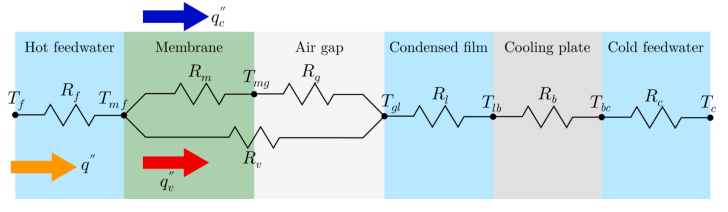
\includegraphics[width=0.5\linewidth]{Imagens//chap03/resistencias.png}
    \caption{}
    \label{fig:placeholder}
\end{figure}

As resistências condutivas consideradas no modelo correspondem à condução de calor através da membrana e do espaço de ar. Para a membrana, a resistência térmica condutiva é dada por:

\begin{equation}
R_m = \frac{\delta_m}{k_m}
\end{equation}

\noindent em que \(R_m\) é a resistência térmica condutiva da membrana, \(\delta_m\) é a espessura da membrana e \(k_m\) é a condutividade térmica da membrana.

Para o espaço de ar, a resistência térmica condutiva é expressa por:

\begin{equation}
R_g = \frac{\delta_g}{k_g}
\end{equation}

\noindent em que \(R_g\) é a resistência térmica condutiva do espaço de ar, \(\delta_g\) é a espessura do espaço de ar e \(k_g\) é a condutividade térmica do ar.

O calor latente associado ao transporte de vapor é expresso por

\begin{equation}
q_v'' = j_w h_{lv}
\end{equation}

em que $q_v''$ é o fluxo de calor latente ($\mathrm{W\,m^{-2}}$), $j_w$ é o fluxo mássico de permeado e $h_{lv}$ é o calor latente de vaporização da água.

A formulação adotada baseia-se em uma analogia com circuitos resistivos para representar os transportes de massa e calor. Nessa analogia, o fluxo é associado a uma força motriz e a uma resistência: para o transporte de massa, a força motriz é a diferença de pressão parcial de vapor; para o transporte de calor, é a diferença de temperatura entre as regiões do módulo.

No caso térmico, a utilização de uma resistência equivalente pressupõe regime estacionário, de modo que o fluxo de calor total seja constante ao longo das camadas consideradas. Nessas condições, as contribuições de convecção, condução e transporte de calor associado ao vapor podem ser representadas por resistências térmicas individuais, cuja combinação fornece uma resistência térmica equivalente para o sistema.

Assim, a resistência térmica equivalente do sistema pode ser escrita genericamente como:


\begin{equation}
R_{eq}
=
R_f +
\frac{R_v (R_m + R_g)}{R_v + R_m + R_g}
+ R_l + R_b + R_c
\end{equation}

\noindent sendo $R_v$, $R_l$ e $R_b$ resistências associadas aos mecanismos de transporte de vapor, condensação e condução estrutural.

O fluxo térmico total entre os canais quente e frio é então

\begin{equation}
q'' = \frac{T_f - T_c}{R_{eq}}
\end{equation}

onde $T_f$ e $T_c$ representam as temperaturas médias das correntes quente e fria.



\subsection{Indicadores de Desempenho Energético}

Além do fluxo de permeado, a avaliação de sistemas de destilação por membranas também pode envolver indicadores energéticos, uma vez que o processo depende do fornecimento de calor para promover a evaporação da água. Entre os indicadores utilizados na literatura estão o consumo específico de energia térmica (\textit{Specific Energy Consumption} -- SEC) e a razão de ganho de saída (\textit{Gain Output Ratio} -- GOR).

O consumo específico de energia térmica representa a quantidade de energia térmica fornecida ao sistema por unidade de volume de permeado produzido. Essa métrica pode ser expressa como a razão entre a taxa de calor externo fornecida ao sistema e a vazão volumétrica de permeado (\cite{curcino2023}):

\begin{equation}
SEC_{th} = \frac{\dot{Q}_{ext}}{\dot{V}_{w}}
\end{equation}

\noindent em que \(SEC_{th}\) é o consumo específico de energia térmica, \(\dot{Q}_{ext}\) é a taxa de calor externo fornecida ao sistema e \(\dot{V}_{w}\) é a vazão volumétrica de permeado produzido.

A razão de ganho de saída, por sua vez, relaciona o calor latente associado à produção de permeado com a energia térmica fornecida ao sistema. Esse indicador é frequentemente utilizado para avaliar o aproveitamento energético do processo, especialmente em sistemas com recuperação de calor:

\begin{equation}
GOR = \frac{\dot{V}_w \rho_w \Delta h_{lv}}{\dot{Q}_{ext}}
\end{equation}

\noindent em que \(GOR\) é a razão de ganho de saída, \(\rho_w\) é a massa específica da água e \(\Delta h_{lv}\) é o calor latente de vaporização.

\section{Modelo Físico Reduzido}

O presente trabalho utiliza como referência o modelo físico reduzido proposto por \cite{Lisboa2024}, desenvolvido para representar o comportamento global de um sistema V-AGMD em escala piloto. Nesta fundamentação teórica, o objetivo não é reproduzir integralmente a formulação apresentada no artigo, mas destacar os aspectos do modelo que são relevantes para a construção da abordagem metodológica adotada neste TCC.

O modelo é classificado como reduzido por representar o módulo por meio de parâmetros concentrados, sem resolver explicitamente perfis espaciais de temperatura, concentração, pressão ou velocidade ao longo dos canais. Dessa forma, o sistema é descrito a partir de grandezas médias ou efetivas, combinadas por balanços globais de massa e energia e por relações de transporte baseadas em resistências equivalentes.

No contexto deste trabalho, o modelo reduzido desempenha três funções principais. Primeiro, fornece uma referência físico-matemática para representar o comportamento esperado do sistema V-AGMD. Segundo, permite comparar as previsões obtidas por modelos orientados por dados com uma formulação baseada em princípios físicos. Terceiro, fornece informação física que pode ser incorporada às abordagens híbridas avaliadas posteriormente.

As principais grandezas estimadas pelo modelo incluem o fluxo de permeado e as temperaturas de saída das correntes do sistema. Essas variáveis são relevantes tanto para a avaliação da produtividade do processo quanto para o cálculo de indicadores energéticos. Assim, o modelo físico reduzido funciona como uma representação fenomenológica simplificada do sistema, conectando os mecanismos de transferência de massa e calor às variáveis de desempenho analisadas neste trabalho.

Por se tratar de uma formulação 0D, o modelo apresenta menor custo computacional quando comparado a modelos distribuídos. Essa característica é importante para sua utilização como referência em um pipeline de modelagem, pois permite gerar estimativas físicas de forma relativamente rápida, sem exigir a resolução detalhada dos campos espaciais no interior do módulo.

Entretanto, as simplificações adotadas também delimitam seu alcance. Como o modelo trabalha com grandezas médias, ele não representa explicitamente variações locais ao longo do módulo, como gradientes axiais de temperatura, concentração e velocidade. Além disso, fenômenos como polarização de concentração, efeitos hidrodinâmicos locais, fouling e alterações estruturais da membrana não são diretamente contemplados.

Dessa forma, neste TCC, o modelo reduzido não é tratado como uma descrição completa do sistema, mas como uma aproximação físico-matemática útil para incorporar conhecimento fenomenológico à modelagem. Suas previsões são utilizadas como referência e como fonte de informação física, sempre considerando as limitações associadas à formulação concentrada e às hipóteses simplificadoras adotadas.
\section{Aprendizado de Máquinas}

O Aprendizado de Máquina (\textit{Machine Learning}) constitui uma abordagem associada à Inteligência Artificial voltada ao desenvolvimento de modelos capazes de aprender a partir de dados observados, identificando padrões e relações que podem ser utilizados para realizar previsões a partir de novos exemplos (\cite{Ghahramani2015}). Diferentemente de modelos baseados em física ou equações, nos quais as relações entre variáveis são formuladas previamente a partir de conhecimento científico, leis de conservação e hipóteses teóricas, os modelos de aprendizado de máquina aprendem relações entrada-saída diretamente dos dados, ajustando seus parâmetros durante o treinamento para minimizar uma função de erro associada à tarefa de interesse (\cite{Rai2020}).

De forma geral, o objetivo do aprendizado de máquinas é estimar uma função que relacione um conjunto de variáveis de entrada a uma variável, ou variáveis, de saída.

Os métodos de aprendizado podem ser classificados em três categorias principais \cite{Sarkar2018PML}:

\begin{itemize}
    \item \textbf{Aprendizado supervisionado}: utiliza dados rotulados, ou seja, pares entrada–saída conhecidos. O modelo aprende uma função que mapeia as entradas nas saídas observadas. Problemas de regressão e classificação pertencem a essa categoria.
    
    \item \textbf{Aprendizado não supervisionado}: opera sobre dados sem rótulos explícitos, buscando identificar padrões estruturais, agrupamentos ou representações latentes.
    
    \item \textbf{Aprendizado por reforço}: baseia-se em interações sequenciais com o ambiente, onde decisões são tomadas visando maximizar uma recompensa acumulada.
\end{itemize}



Diversas técnicas foram desenvolvidas para tarefas supervisionadas, incluindo regressão linear, modelos regularizados, árvores de decisão, métodos baseados em \textit{ensembles} e redes neurais artificiais. Cada uma dessas abordagens apresenta características distintas quanto à complexidade, capacidade de generalização e interpretabilidade, aspectos que serão discutidos nas seções seguintes.

\subsection{Formulação do Problema de Regressão}

Em regressão supervisionada, assume-se que os dados observados são gerados a partir de um modelo estatístico da forma

\begin{equation}
Y = f(X) + \varepsilon,
\end{equation}

onde $X$ representa o vetor de variáveis de entrada, $Y$ é a variável resposta e $\varepsilon$ é um termo de erro aleatório tal que $E(\varepsilon)=0$ e $\varepsilon$ é independente de $X$ (\cite{Sarkar2018PML}). Nesse modelo, a função verdadeira $f(x)$ coincide com a média condicional:

\begin{equation}
f(x) = E(Y \mid X = x).
\end{equation}

O objetivo do aprendizado é estimar uma função \(\hat{f}\), a partir de um conjunto finito de observações \(\{(x_i, y_i)\}_{i=1}^{N}\), capaz de produzir boas previsões para novos valores de entrada dentro da faixa de operação coberta pelo conjunto de treinamento.

\subsubsection*{Perda Quadrática e Erro Esperado de Predição}

Para quantificar erros de predição, introduz-se uma função de perda $L(Y,f(X))$. A forma mais comum é a perda quadrática,

\begin{equation}
L(Y,f(X)) = (Y - f(X))^2.
\end{equation}

Sob essa escolha, define-se o erro esperado de predição (do inglês, \textit{Expected Prediction Error}) como

\begin{equation}
EPE(f) = E[(Y - f(X))^2],
\end{equation}

onde a expectativa é tomada sobre a distribuição conjunta de $(X,Y)$. Pode-se escrever equivalentemente

\begin{equation}
EPE(f) = E_X \, E_{Y|X} \left[(Y - f(X))^2 \mid X \right].
\end{equation}

A minimização do EPE pode ser realizada ponto a ponto em $x$, resultando em

\begin{equation}
f(x) = \arg\min_c E_{Y|X} \left[(Y - c)^2 \mid X = x \right].
\end{equation}

A solução desse problema é dada pela média condicional,

\begin{equation}
f(x) = E(Y \mid X = x),
\end{equation}

mostrando que, sob perda quadrática, a melhor predição possível é a média condicional da variável resposta.

\subsubsection*{Erro de Treinamento e Generalização}

Na prática, a distribuição verdadeira dos dados é desconhecida, de modo que o EPE não pode ser calculado diretamente. Em seu lugar, utiliza-se o erro de treinamento, definido pelo critério de soma de quadrados dos resíduos, definido por:

\begin{equation}
RSS(f) = \sum_{i=1}^{N} (y_i - f(x_i))^2.
\end{equation}

A minimização do $RSS$ produz um estimador ajustado aos dados observados. Entretanto, um modelo que apresenta erro de treinamento muito baixo pode não apresentar desempenho equivalente em novos pontos de teste. O erro esperado em novas observações — também chamado de erro de teste ou erro de generalização — corresponde ao EPE avaliado em dados independentes do conjunto de treinamento.

Essa distinção entre erro de treinamento e erro de teste é fundamental para a análise do desempenho preditivo e será explorada nas seções seguintes.

\subsection{Métricas de Avaliação para Regressão}

A avaliação do desempenho preditivo dos modelos de regressão é realizada por meio de funções de perda ou funções de pontuação (do inglês, \textit{scoring functions}), que quantificam a discrepância entre os valores observados $y_i$ e as previsões $\hat{y}_i$. 

As funções de pontuação são ferramentas padrão para avaliação de modelos, sendo exemplos clássicos o erro quadrático e o erro absoluto (\cite{Fissler2022ModelComparison}). No contexto deste trabalho, foram consideradas métricas amplamente utilizadas em problemas de regressão, uma vez que as variáveis de interesse, como fluxo de permeado e temperaturas de saída, são contínuas. Assim, o erro quadrático médio (MSE), a raiz do erro quadrático médio (RMSE), o erro absoluto médio (MAE), o erro percentual absoluto médio (MAPE) e o coeficiente de determinação (\(R^2\)) foram utilizados por fornecerem avaliações complementares do desempenho preditivo.

O MSE e o RMSE penalizam mais fortemente erros de maior magnitude, sendo úteis para identificar modelos com grandes desvios de previsão. O MAE fornece uma medida direta do erro médio absoluto, com menor sensibilidade a desvios extremos. O MAPE expressa o erro em termos relativos, permitindo interpretar o desvio percentual entre previsões e valores observados. Já o \(R^2\) avalia a proporção da variabilidade dos dados explicada pelo modelo. Dessa forma, a combinação dessas métricas permite analisar não apenas a magnitude dos erros, mas também a qualidade global do ajuste obtido pelos modelos.

\subsubsection{Erro Quadrático Médio (MSE)}

O erro quadrático médio ( do inglês, \textit{Mean Squared Error} -- MSE) mede a média dos quadrados das diferenças entre os valores observados e os valores previstos pelo modelo. Para um conjunto com \(N\) observações, essa métrica é definida como:

\begin{equation}
MSE = \frac{1}{N}\sum_{i=1}^{N}(y_i - \hat{y}_i)^2,
\end{equation}

\noindent em que \(y_i\) representa o valor observado da variável de saída para a amostra \(i\), \(\hat{y}_i\) representa o valor previsto pelo modelo para essa mesma amostra e \(N\) é o número total de observações.
\subsubsection*{Raiz do Erro Quadrático Médio (RMSE)}

A raiz do erro quadrático médio é definida como:

\begin{equation}
\mathrm{RMSE} = \sqrt{\mathrm{MSE}}.
\end{equation}

A aplicação da raiz quadrada constitui uma transformação monotônica, de modo que MSE e RMSE induzem a mesma ordenação de modelos. A principal vantagem do RMSE é expressar o erro na mesma unidade da variável resposta, facilitando sua interpretação física (\cite{Fissler2022ModelComparison}).

\subsubsection*{Erro Absoluto Médio (MAE)}

A função de perda absoluta é definida como:

\begin{equation}
L(z,y) = |z - y|.
\end{equation}

O erro absoluto médio (Mean Absolute Error, MAE) é dado por:

\begin{equation}
\mathrm{MAE} = \frac{1}{n} \sum_{i=1}^{n} |\hat{y}_i - y_i|.
\end{equation}

O erro absoluto é estritamente consistente para o funcional mediana condicional. Diferentemente do MSE, o MAE não eleva os erros ao quadrado, tornando-o menos sensível a valores extremos. Sua unidade coincide com a unidade da variável resposta (\cite{Fissler2022ModelComparison}).

\subsubsection*{Erro Percentual Absoluto Médio (MAPE)}

O erro percentual absoluto é definido como:

\begin{equation}
\mathrm{APE}_i = \left| \frac{y_i - \hat{y}_i}{y_i} \right|.
\end{equation}

O erro percentual absoluto médio (MAPE) é então:

\begin{equation}
\mathrm{MAPE} = \frac{1}{n} \sum_{i=1}^{n} 
\left| \frac{y_i - \hat{y}_i}{y_i} \right|.
\end{equation}

Essa métrica é adimensional, permitindo comparação relativa entre diferentes variáveis. Entretanto, apresenta limitações quando $y_i$ assume valores próximos de zero, podendo gerar instabilidades numéricas.

\subsubsection*{Coeficiente de Determinação ($R^2$)}

O coeficiente de determinação mede a proporção da variância da variável resposta explicada pelo modelo. Para um conjunto com $n$ observações, é definido por:

\begin{equation}
R^2 = 1 - 
\frac{\sum_{i=1}^{n}(y_i - \hat{y}_i)^2}
{\sum_{i=1}^{n}(y_i - \bar{y})^2},
\end{equation}

onde $\bar{y}$ representa a média amostral:

\begin{equation}
\bar{y} = \frac{1}{n}\sum_{i=1}^{n} y_i.
\end{equation}

O valor máximo de $R^2$ é 1, indicando ajuste perfeito. Valores negativos podem ocorrer quando o modelo apresenta desempenho inferior ao de um modelo constante que sempre prediz a média amostral.

O $R^2$ fornece uma medida de qualidade de ajuste baseada na variância explicada, sendo amplamente utilizado em problemas de regressão.

\subsection{Correlação, Associação Estatística e Causalidade}
\label{subsec:correlacao_associacao_causalidade}

A análise de correlação é uma ferramenta estatística utilizada para investigar a associação entre duas variáveis. No contexto deste trabalho, essa análise é empregada de forma exploratória, com o objetivo de identificar tendências gerais entre as variáveis operacionais de entrada e as variáveis de saída do sistema V-AGMD. Entretanto, diferentes coeficientes de correlação capturam diferentes tipos de associação, sendo importante distinguir suas interpretações.

O coeficiente de correlação de Pearson, usualmente representado por \(r\), é associado à análise de relações lineares entre duas variáveis quantitativas. Valores positivos indicam que as variáveis tendem a aumentar conjuntamente, enquanto valores negativos indicam que uma variável tende a diminuir quando a outra aumenta. Valores próximos de zero indicam ausência de associação linear forte, embora não excluam a possibilidade de relações não lineares. Dessa forma, o coeficiente de Pearson é mais adequado quando se deseja avaliar a presença de uma tendência aproximadamente linear entre as variáveis.

O coeficiente de correlação de Spearman, usualmente representado por \(\rho\), é calculado a partir dos postos, ou posições ordenadas, das observações. Por esse motivo, ele é frequentemente utilizado para avaliar associações monotônicas, isto é, situações em que uma variável tende a aumentar ou diminuir de forma consistente em relação à outra, ainda que a relação não seja necessariamente linear. Assim, Spearman pode ser mais apropriado em análises exploratórias nas quais se deseja identificar tendências crescentes ou decrescentes sem impor uma forma linear específica à relação entre as variáveis. (\cite{VanDenHeuvel2022Correlation})

Apesar dessa distinção, ambos os coeficientes devem ser interpretados como medidas de associação estatística. Eles indicam o grau e a direção de uma relação observada entre variáveis, mas não estabelecem, por si só, uma relação de causa e efeito. Como discutido por \cite{Holland1986StatisticsCausal}, correlação não implica causalidade: a observação de que duas variáveis variam conjuntamente não significa necessariamente que uma delas cause a outra. A associação observada pode decorrer de efeitos indiretos, de variáveis não consideradas, de restrições impostas pelo planejamento experimental ou da combinação simultânea de múltiplas condições operacionais.

Essa distinção é particularmente relevante porque as análises de dispersão e correlação são utilizadas como ferramentas exploratórias para apoiar a compreensão inicial dos dados. Assim, eventuais associações observadas entre variáveis de entrada e saída não são interpretadas como evidência causal isolada. As conclusões do estudo concentram-se na capacidade preditiva dos modelos avaliados e na identificação de padrões estatísticos dentro do domínio experimental analisado, sem assumir que as correlações observadas estabeleçam relações causais diretas entre as variáveis.

\subsubsection*{Considerações para Regressão Multi-Output}

No caso de regressão com múltiplas saídas, as métricas são calculadas individualmente para cada variável dependente. Essa abordagem permite avaliar o desempenho do modelo de forma específica para cada grandeza física prevista, evitando mascaramento de erros devido a diferenças de escala entre as variáveis.

Nas subseções seguintes, são apresentados o procedimento clássico de validação cruzada por \(K\) partições e a adaptação baseada em grupos, utilizada neste trabalho para respeitar a estrutura dos regimes operacionais.

\subsection{Controle de Complexidade e Overfitting}

O desempenho preditivo de um modelo supervisionado está diretamente relacionado ao seu grau de complexidade. Em problemas de regressão, assume-se tipicamente que os dados são gerados segundo

\begin{equation}
Y = f(X) + \varepsilon,
\end{equation}

onde $f(X)$ é a função verdadeira desconhecida e $\varepsilon$ é um termo de ruído com $E(\varepsilon)=0$ e $Var(\varepsilon)=\sigma_\varepsilon^2$. O objetivo do aprendizado é construir um estimador $\hat{f}(X)$ capaz de aproximar $f(X)$ a partir de um conjunto finito de dados. \cite{Hastie2009ESL}


\subsubsection{Complexidade do Modelo, Overfitting e Underfitting}

A flexibilidade de um modelo está associada à sua capacidade de se ajustar a diferentes formas funcionais entre as variáveis de entrada e a variável de saída. Modelos pouco flexíveis tendem a representar relações mais simples, enquanto modelos mais flexíveis conseguem capturar padrões mais complexos e não lineares nos dados. Entretanto, o aumento da flexibilidade também pode tornar o modelo mais sensível às particularidades do conjunto de treinamento, elevando o risco de \textit{overfitting} quando não há controle adequado de complexidade (\cite{Hastie2009ESL}).


Entretanto, essa maior flexibilidade pode levar ao fenômeno de \textit{overfitting}, no qual o modelo passa a capturar não apenas o padrão estrutural dos dados, mas também flutuações aleatórias específicas da amostra de treinamento. Nesse caso, o erro de treinamento tende a ser baixo, pois o modelo se ajusta muito bem aos dados utilizados no seu ajuste. No entanto, o erro de generalização pode ser elevado, uma vez que o modelo passa a ter dificuldade para realizar boas previsões em dados novos, não utilizados durante o treinamento. Assim, a diferença entre esses erros está no conjunto de dados considerado: o erro de treinamento é calculado sobre os dados usados para ajustar o modelo, enquanto o erro de generalização representa o desempenho esperado em novas observações.

Por outro lado, modelos excessivamente restritivos podem apresentar \textit{underfitting}, caracterizado por alto erro tanto no treinamento quanto na validação, devido à incapacidade de representar adequadamente a função subjacente.

Existe, portanto, um nível intermediário de complexidade que minimiza o erro esperado de predição.

\subsubsection{Decomposição Viés--Variância}

Sob perda quadrática, o erro esperado de predição em um ponto $x_0$ pode ser decomposto como

\begin{equation}
Err(x_0) = \sigma_\varepsilon^2 
+ \left[ E\hat{f}(x_0) - f(x_0) \right]^2 
+ E\left[ \hat{f}(x_0) - E\hat{f}(x_0) \right]^2.
\end{equation}

Os termos correspondem a:

\begin{itemize}
\item \textbf{Erro irredutível} ($\sigma_\varepsilon^2$): variabilidade inerente ao processo gerador dos dados;
\item \textbf{Viés ao quadrado}: erro sistemático introduzido pelas restrições do modelo;
\item \textbf{Variância}: sensibilidade do modelo às flutuações do conjunto de treinamento.
\end{itemize}

De modo geral, o aumento da complexidade reduz o viés, pois amplia o conjunto de funções representáveis, mas aumenta a variância, tornando o modelo mais sensível às particularidades da amostra. O erro total resulta do equilíbrio entre esses dois efeitos.


\subsubsection{Espaço do Modelo}

O espaço do modelo pode ser definido como o conjunto de todas as previsões possíveis que podem ser produzidas pelo procedimento de aprendizado. Modelos mais flexíveis possuem um espaço de hipóteses mais amplo, enquanto modelos mais restritivos operam em um subconjunto reduzido desse espaço.

A ampliação do espaço do modelo tende a reduzir o viés estrutural, porém aumenta a variabilidade das estimativas obtidas a partir de diferentes amostras.

\subsubsection{Regularização baseada em física}

A regularização é uma estratégia utilizada para controlar a complexidade do modelo e melhorar sua capacidade de generalização. Em termos gerais, ela consiste na introdução de penalizações associadas à complexidade ou à suavidade da função ajustada, restringindo a flexibilidade do modelo e reduzindo a tendência de ajuste excessivo aos dados de treinamento (\cite{Tian2022}).

Em modelos híbridos ou físico-informados, essa ideia pode ser estendida pela incorporação de termos associados ao conhecimento físico na função de perda. Nabian e Meidani propõem uma regularização orientada pela física na qual a função objetivo combina um termo de ajuste aos dados com um termo baseado no resíduo das equações governantes do sistema. Esse termo adicional penaliza desvios em relação às leis físicas conhecidas, induzindo o modelo a produzir soluções mais consistentes com o comportamento esperado do sistema (\cite{Nabian2020}).

Dessa forma, a regularização baseada em física pode ser interpretada como uma restrição adicional ao espaço de soluções admissíveis. Além de reduzir o erro em relação aos dados experimentais, o modelo passa a ser penalizado quando suas previsões violam relações físicas conhecidas. Essa estratégia é particularmente relevante em problemas com poucos dados rotulados ou com forte estrutura física subjacente, pois permite incorporar conhecimento fenomenológico ao treinamento e reduzir a ocorrência de previsões fisicamente inconsistentes (\cite{Nabian2020}).
\subsubsection{Graus de Liberdade Efetivos}

Em modelos gerais, a complexidade pode ser quantificada por meio dos graus de liberdade efetivos, que medem o grau de adaptação do modelo aos dados observados. Diferentemente do simples número de parâmetros, os graus de liberdade efetivos capturam a flexibilidade real do procedimento de ajuste, sendo aplicáveis também a métodos não paramétricos.

Essa noção fornece uma métrica unificada para comparar o nível de complexidade entre diferentes famílias de modelos.




\subsection{Validação Cruzada}
\label{sec:validacao_cruzada}

A avaliação de modelos supervisionados busca estimar sua capacidade de generalização, isto é, seu desempenho em observações não utilizadas durante o treinamento. De forma geral, esse desempenho pode ser associado ao erro esperado de predição extra-amostral. Conforme discutido em \cite{Hastie2009ESL}, esse erro pode ser expresso por

\begin{equation}
\mathrm{Err} = \mathbb{E}[L(Y,\hat{f}(X))],
\label{eq:erro_esperado_generalizacao}
\end{equation}

\noindent em que \(L(Y,\hat{f}(X))\) representa a função de perda entre o valor observado \(Y\) e a predição obtida pelo modelo \(\hat{f}(X)\). A expectativa é tomada sobre novas observações provenientes da mesma distribuição conjunta de \((X,Y)\).

Na prática, como a distribuição verdadeira dos dados é desconhecida, o erro de generalização não pode ser observado diretamente e precisa ser estimado a partir do conjunto de dados disponível. Assim, os procedimentos de validação buscam fornecer estimativas empíricas do desempenho preditivo esperado, permitindo comparar modelos, selecionar hiperparâmetros e avaliar a capacidade de generalização das soluções obtidas.

\subsubsection*{Divisão treino--teste}

Uma estratégia simples para estimar o desempenho de generalização é a divisão treino--teste, também associada à abordagem de validação por conjunto separado. Nesse procedimento, a base de dados é particionada em subconjuntos disjuntos, de modo que uma parte dos dados seja utilizada para o ajuste do modelo e outra parte seja reservada para avaliar seu desempenho em observações não empregadas no treinamento.

Em uma formulação mais completa, pode-se ainda separar os dados em três subconjuntos: treinamento, validação e teste. O conjunto de treinamento é utilizado para ajustar os parâmetros do modelo, o conjunto de validação auxilia na escolha de modelos ou hiperparâmetros, e o conjunto de teste deve ser reservado para a avaliação final do modelo selecionado. Como discutido por \cite{Hastie2009ESL}, o conjunto de teste deve ser mantido separado até o final da análise, pois seu uso repetido durante a seleção pode levar a uma estimativa excessivamente otimista do erro de generalização.

Apesar de sua simplicidade, essa estratégia pode ser limitada quando o número de observações disponíveis é reduzido. Nesses casos, a separação da base em múltiplos subconjuntos diminui a quantidade de dados disponível para o ajuste do modelo e pode tornar a avaliação sensível à composição dos subconjuntos utilizados. Por esse motivo, métodos baseados em reutilização eficiente da amostra, como a validação cruzada e o bootstrap, são frequentemente empregados em situações nas quais não há dados suficientes para uma divisão convencional em conjuntos de treinamento, validação e teste (\cite{Hastie2009ESL}).

\begin{figure}[H]
    \centering
    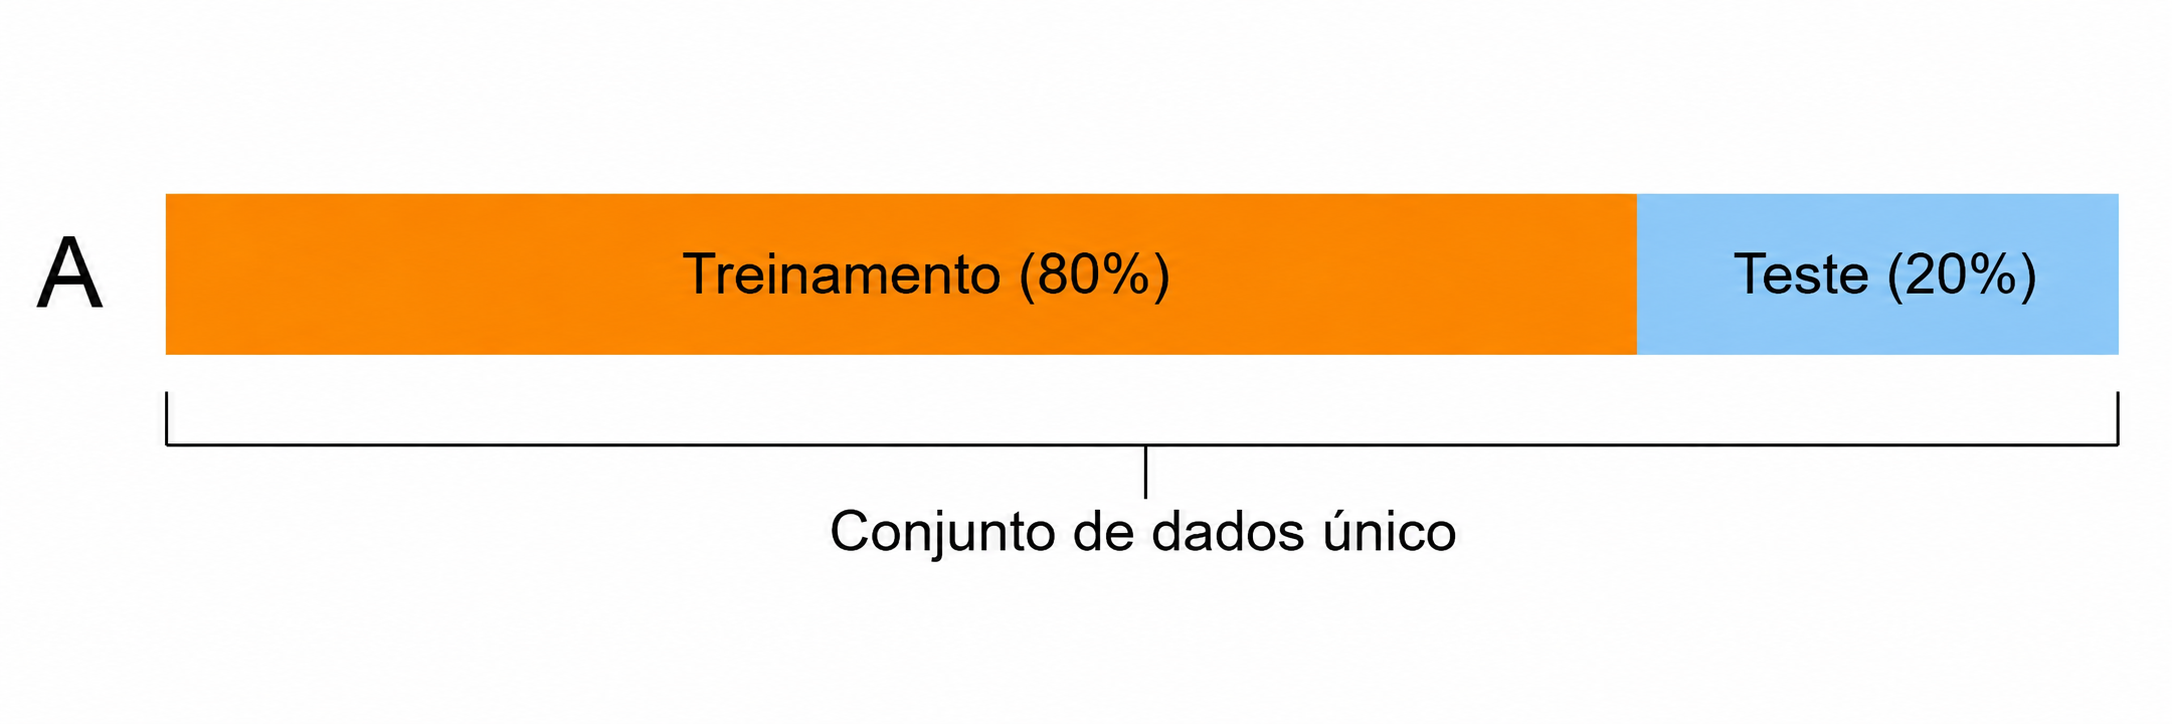
\includegraphics[width=0.75\linewidth]{Imagens/chap04/8020.png}
    \caption[Divisão treino--teste 80/20]{Representação esquemática da divisão treino--teste simples na proporção 80/20. Nessa estratégia, o conjunto de dados é separado uma única vez em dois subconjuntos: 80\% das observações são utilizadas para treinamento do modelo e 20\% são reservadas para avaliação do desempenho preditivo, sem serem utilizadas no ajuste dos parâmetros do modelo. Fonte: Elaborado pela autora.}
    \label{fig:divisao_treino_teste_80_20}
\end{figure}
\subsubsection*{Validação Cruzada \(K\)-Fold}

Na validação cruzada \(K\)-fold, o conjunto de dados é dividido em \(K\) subconjuntos aproximadamente do mesmo tamanho. Para cada partição \(k = 1, \dots, K\), o modelo é ajustado utilizando \(K-1\) subconjuntos, enquanto o subconjunto restante é utilizado para validação. O processo é repetido até que todos os subconjuntos tenham sido utilizados uma vez como conjunto de validação.

Formalmente, seja \(k(i)\) a função que indica a qual subconjunto pertence a observação \(i\), e seja \(\hat{f}^{-k(i)}\) o modelo ajustado excluindo o subconjunto \(k(i)\). A estimativa de validação cruzada é dada por

\begin{equation}
\mathrm{CV}(\hat{f}) =
\frac{1}{N}
\sum_{i=1}^{N}
L\big(y_i, \hat{f}^{-k(i)}(x_i)\big).
\label{eq:cv_estimativa}
\end{equation}

Quando o modelo depende de um hiperparâmetro \(\alpha\), a estimativa pode ser escrita como

\begin{equation}
\mathrm{CV}(\hat{f},\alpha) =
\frac{1}{N}
\sum_{i=1}^{N}
L\big(y_i, \hat{f}^{-k(i)}(x_i,\alpha)\big).
\label{eq:cv_hiperparametro}
\end{equation}

Nesse caso, o valor de \(\alpha\) que minimiza \(\mathrm{CV}(\hat{f},\alpha)\) pode ser selecionado, e o modelo final é então ajustado utilizando todos os dados disponíveis com esse hiperparâmetro. Valores usuais de \(K\) são 5 ou 10, representando um compromisso prático entre estabilidade da estimativa e custo computacional (\cite{Hastie2009ESL}).

\begin{figure}[H]
    \centering
    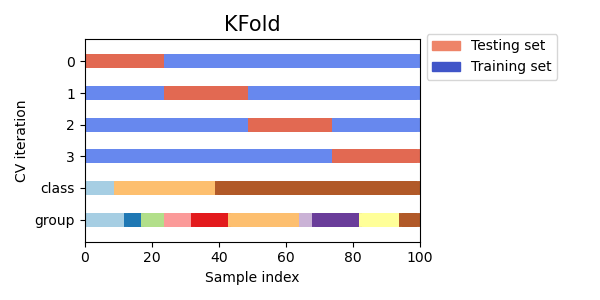
\includegraphics[width=0.75\linewidth]{Imagens/chap04/k-fold.png}
    \caption[Validação cruzada \(K\)-fold]{Representação esquemática da validação cruzada \(K\)-fold. O conjunto de dados é dividido em \(K\) partições e, a cada iteração, uma partição é utilizada para validação enquanto as demais são utilizadas para treinamento. Fonte: \cite{sklearn_groupkfold_docs}}
    \label{fig:kfold_validacao}
\end{figure}

\subsubsection*{Validação Cruzada Agrupada}

Em alguns conjuntos de dados, as observações não podem ser consideradas completamente independentes entre si. Isso ocorre, por exemplo, quando diferentes amostras pertencem a um mesmo grupo experimental, indivíduo, unidade de ensaio, condição operacional ou regime de operação. Nesses casos, uma validação cruzada aleatória pode distribuir observações correlacionadas simultaneamente entre treinamento e validação, produzindo estimativas excessivamente otimistas de desempenho.

Para lidar com essa limitação, pode-se utilizar a validação cruzada agrupada. Nessa estratégia, os grupos definidos pelo usuário são tratados como unidades indivisíveis durante o particionamento dos dados. Assim, todas as observações pertencentes a um mesmo grupo são alocadas integralmente no conjunto de treinamento ou no conjunto de validação em cada iteração. Esse procedimento permite avaliar a capacidade do modelo de generalizar para grupos não utilizados durante o ajuste, reduzindo o risco de que informações associadas a um mesmo grupo experimental estejam presentes simultaneamente nos subconjuntos de treinamento e validação.

% CITAÇÃO A VERIFICAR:
% A documentação do scikit-learn pode sustentar a descrição operacional do GroupKFold.
% Para fundamentação acadêmica, buscar uma fonte sobre grouped cross-validation,
% clustered data, repeated measurements ou dependência entre observações experimentais.

\begin{figure}[H]
    \centering
    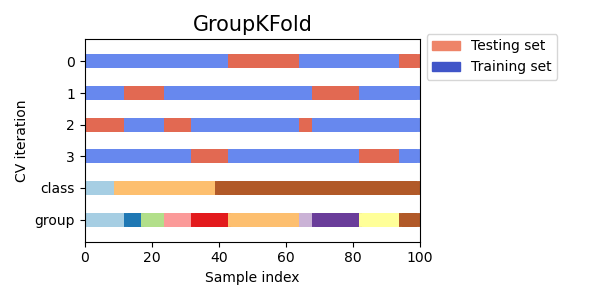
\includegraphics[width=0.75\linewidth]{Imagens/chap04/group_k_fold.png}
    \caption[Validação cruzada agrupada]{Representação esquemática da validação cruzada agrupada. Nesse procedimento, todas as observações pertencentes a um mesmo grupo experimental são mantidas na mesma partição, evitando que amostras correlacionadas sejam distribuídas simultaneamente entre treinamento e validação. Fonte: \cite{sklearn_groupkfold_docs}}
    \label{fig:groupkfold_validacao}
\end{figure}

\subsubsection*{Incerteza na Estimação do Desempenho Preditivo}

Embora a validação cruzada seja amplamente utilizada para estimar o desempenho preditivo de modelos, sua interpretação exige cuidado. A estimativa obtida por validação cruzada não deve ser entendida como uma medida exata do erro de predição do modelo final ajustado aos dados observados. Como discutido por \cite{Bates2022CV}, a validação cruzada estima, de forma mais adequada, o erro médio esperado de modelos ajustados a diferentes conjuntos de treinamento hipotéticos provenientes da mesma distribuição, e não necessariamente o erro específico do modelo ajustado à amostra disponível.

No contexto da validação cruzada com \(K\) partições, seja \(\mathcal{L}^{(k)}_{\mathrm{val}}\) a métrica de validação obtida na partição \(k\). A média das métricas de validação é dada por

\begin{equation}
\overline{\mathcal{L}}_{\mathrm{val}} =
\frac{1}{K}\sum_{k=1}^{K} \mathcal{L}^{(k)}_{\mathrm{val}}.
\label{eq:media_validacao}
\end{equation}

\noindent Essa média fornece uma estimativa pontual do desempenho preditivo esperado associado ao procedimento de modelagem avaliado. Entretanto, como as métricas podem variar entre as partições, é importante considerar também a dispersão dos resultados obtidos ao longo da validação cruzada. De forma prática, essa variabilidade pode ser resumida por meio do erro padrão:

\begin{equation}
\mathrm{SE}(\overline{\mathcal{L}}_{\mathrm{val}}) =
\frac{\sigma(\mathcal{L}_{\mathrm{val}})}{\sqrt{K}},
\label{eq:erro_padrao_validacao}
\end{equation}

\noindent em que \(\sigma(\mathcal{L}_{\mathrm{val}})\) representa o desvio padrão das métricas de validação obtidas nas \(K\) partições.

Essa medida, contudo, deve ser interpretada como uma aproximação prática da variabilidade observada entre partições, e não como uma caracterização exata da incerteza estatística do erro de generalização. Intervalos de confiança ingênuos derivados da validação cruzada podem apresentar cobertura inferior à nominal, pois estimativas de erro obtidas em diferentes partições não são completamente independentes, havendo correlação entre elas devido ao reaproveitamento dos dados nos processos de treinamento e validação \cite{Bates2022CV}. De forma complementar, \cite{BengioGrandvalet2003VarianceKFold} mostram que a estimação da variância do estimador de validação cruzada é um problema não trivial, não existindo estimador não viesado dessa variância a partir de uma única execução de validação cruzada.

O erro padrão calculado entre partições pode ser utilizado como uma medida prática da dispersão das métricas de validação, auxiliando a comparação entre modelos e a formulação de critérios de seleção que considerem a variabilidade da estimativa. Entretanto, essa medida deve ser interpretada com cautela: ela não corresponde a um intervalo de confiança exato para o desempenho real de generalização, mas a um indicador aproximado da variabilidade associada à avaliação em amostras finitas.


\subsubsection*{Sobreajuste no Processo de Seleção de Modelos}

A validação cruzada é frequentemente utilizada não apenas para estimar desempenho, mas também como critério de seleção de modelos, hiperparâmetros ou arquiteturas. Nesse caso, o processo de seleção passa a depender diretamente de uma estimativa de desempenho de generalização, como o erro médio obtido por validação cruzada. Como esse critério possui componentes de viés e variância, a escolha da configuração com menor erro médio pode favorecer modelos que apresentam desempenho aparentemente superior devido à variabilidade da estimativa, e não necessariamente por melhor capacidade real de generalização (\cite{Cawley2010Overfitting}).

Esse fenômeno é conhecido na literatura como sobreajuste no processo de seleção de modelos. Ele ocorre quando a otimização entre múltiplas configurações explora a variabilidade presente no critério de validação, selecionando uma alternativa que se ajusta excessivamente às particularidades da amostra ou das partições utilizadas na avaliação. Como consequência, o desempenho estimado para o modelo selecionado pode apresentar viés de seleção e viés otimista em relação ao desempenho esperado em dados verdadeiramente novos (\cite{Cawley2010Overfitting}).

Esse risco tende a ser mais pronunciado quando o conjunto de dados é pequeno, quando o critério de seleção apresenta variância não desprezível ou quando o número de hiperparâmetros a serem ajustados é relativamente grande. Nesses casos, a busca por configurações ótimas pode se tornar mais sensível às flutuações do critério de validação, aumentando a chance de selecionar uma configuração que parece superior na amostra analisada, mas que não necessariamente generaliza melhor (\cite{Cawley2010Overfitting}).

Para mitigar esse problema, a seleção de modelos deve ser tratada como parte integrante do próprio processo de ajuste do modelo, sendo refeita sempre que o procedimento for aplicado a uma nova amostra de dados. Essa perspectiva evita que a avaliação de desempenho desconsidere a variabilidade introduzida pela etapa de seleção e reduz o risco de estimativas excessivamente otimistas (\cite{Cawley2010Overfitting}).

Além disso, regras de seleção parcimoniosas podem ser utilizadas quando o objetivo é escolher uma configuração robusta, evitando favorecer modelos mais complexos cuja melhora de desempenho esteja dentro da incerteza da estimativa. Entre essas regras, destaca-se a regra do \textit{one-standard-error}, discutida a seguir.
% CITAÇÃO A VERIFICAR:
% Fonte sugerida: \cite{Hastie2009ESL}.
% Buscar também Yates2021Parsimonious ou Yates2023CV, caso sejam usadas
% para justificar seleção parcimoniosa considerando incerteza.
\subsubsection*{Seleção de Modelos pela Regra do \textit{One-Standard-Error}}

A regra do \textit{one-standard-error} é uma estratégia de seleção parcimoniosa baseada nas estimativas de validação cruzada. Em vez de escolher necessariamente o modelo com menor erro médio, esse critério seleciona o modelo mais simples cujo desempenho esteja dentro de uma margem de um erro padrão em relação ao melhor modelo observado. (\cite{Yates2022})

Para métricas de erro, identifica-se inicialmente o modelo \(m^\ast\) com menor erro médio de validação. Em seguida, considera-se elegível qualquer modelo \(m\) que satisfaça

\begin{equation}
\overline{\mathcal{L}}_{\mathrm{val}}(m)
\leq
\overline{\mathcal{L}}_{\mathrm{val}}(m^\ast)
+
\mathrm{SE}\left(\overline{\mathcal{L}}_{\mathrm{val}}(m^\ast)\right),
\label{eq:one_standard_error}
\end{equation}

\noindent em que \(m^\ast\) representa o modelo com menor erro médio de validação, \(\overline{\mathcal{L}}_{\mathrm{val}}(m^\ast)\) é esse menor erro médio, e \(m\) representa um modelo candidato cujo erro médio está dentro do limite de um erro padrão em relação ao melhor modelo.

Entre os modelos que satisfazem essa condição, seleciona-se aquele de menor complexidade. Dessa forma, a regra do \textit{one-standard-error} evita favorecer modelos mais complexos quando sua melhora de desempenho está dentro da variabilidade da estimativa de validação cruzada (\cite{Hastie2009ESL}).

A noção de menor complexidade depende da família de modelos considerada, podendo estar associada, por exemplo, à intensidade da regularização, à profundidade de árvores, ao número de estimadores, ao número de parâmetros ajustáveis ou ao tamanho de uma arquitetura neural. Portanto, a regra não define a complexidade de forma universal, mas estabelece um critério geral de seleção parcimoniosa a partir das estimativas de validação cruzada.
\subsection{Estratégias de Pré-processamento e Engenharia de Dados}

O desempenho de modelos de aprendizado supervisionado pode ser significativamente influenciado pelas etapas de pré-processamento e engenharia de atributos. O pré-processamento corresponde ao conjunto de procedimentos aplicados aos dados antes do treinamento, com o objetivo de padronizar escalas, reduzir inconsistências, tratar ruídos ou adequar as variáveis ao algoritmo utilizado. Já a engenharia de atributos envolve a transformação, seleção ou construção de variáveis de entrada, buscando representar melhor as informações relevantes para o processo de modelagem.

Nesta seção, são apresentadas algumas ferramentas de tratamento e preparação dos dados utilizadas ou avaliadas neste trabalho, incluindo discretização de variáveis contínuas, escalonamento, seleção de atributos e geração sintética de dados. Essas técnicas podem contribuir para melhorar a estabilidade numérica dos modelos, reduzir redundâncias, capturar relações não lineares e favorecer a capacidade de generalização.

\subsubsection{Binning (Discretização de Variáveis Contínuas)}

O \textit{binning}, também denominado discretização ou quantização, consiste na transformação de variáveis numéricas contínuas em variáveis discretas por meio da divisão de seu domínio em intervalos (bins). Cada intervalo representa uma faixa de valores e recebe um rótulo ou código discreto.

Conforme descrito em \cite{Sarkar2018PML}, a discretização pode ser realizada por meio de esquemas de largura fixa ( do inglês, \textit{fixed-width binning}) ou por estratégias adaptativas, como discretização baseada em quantis, nas quais os limites dos intervalos são definidos com base na própria distribuição dos dados.

Formalmente, dada uma variável contínua \(x \in \mathbb{R}\), define-se uma partição do seu domínio em \(K\) intervalos disjuntos:
\[
I_1, I_2, \dots, I_K,
\]
tal que
\[
\bigcup_{k=1}^{K} I_k = \mathrm{dom}(x)
\quad \text{e} \quad
I_i \cap I_j = \emptyset \ \text{para} \ i \neq j.
\]

\noindent em que \(x\) representa a variável contínua a ser discretizada, \(\mathbb{R}\) representa o conjunto dos números reais, \(K\) é o número total de intervalos definidos, \(I_k\) representa o \(k\)-ésimo intervalo da partição, \(\mathrm{dom}(x)\) é o domínio da variável \(x\), e \(I_i \cap I_j = \emptyset\) indica que os intervalos são disjuntos, isto é, não possuem elementos em comum quando \(i \neq j\).

Cada observação \(x\) é então mapeada para o índice do intervalo ao qual pertence.

A discretização pode ser particularmente útil quando a variável contínua apresenta distribuição assimétrica, caudas longas ou concentração de observações em determinadas faixas de valores. Nesses casos, a transformação em intervalos pode facilitar a representação da estrutura dos dados, reduzindo a influência de variações muito pequenas dentro de uma mesma faixa. Além disso, essa técnica pode ser empregada quando se deseja capturar relações não lineares de forma simplificada, especialmente em modelos que se beneficiam de representações por faixas em vez de relações estritamente contínuas ou lineares.

\paragraph{Risco de perda de informação}

Apesar de suas possíveis vantagens, a discretização implica em perda de informação. Ao substituir um valor contínuo por um identificador de intervalo, elimina-se a variação interna dentro de cada bin.

Esse processo pode:

\begin{itemize}
    \item Reduzir a resolução da variável;
    \item Introduzir descontinuidades artificiais;
    \item Aumentar a dimensionalidade quando utilizada codificação categórica;
    \item Gerar instabilidade caso os limites dos bins não possuam fundamentação estatística ou física.
\end{itemize}

Assim, a aplicação de binning deve ser cuidadosamente avaliada, considerando tanto seus potenciais ganhos de modelagem quanto os riscos associados à perda de granularidade dos dados.

\subsubsection{Padronização e Escalonamento de Variáveis}

Em problemas de aprendizado de máquina envolvendo variáveis numéricas contínuas, é comum que diferentes atributos apresentem ordens de grandeza significativamente distintas. Algumas variáveis podem assumir valores muito elevados, enquanto outras permanecem em faixas reduzidas. O uso direto dessas variáveis pode introduzir viés numérico no processo de treinamento, favorecendo atributos com maior magnitude.

Conforme discutido em \cite{Sarkar2018PML}, muitos algoritmos são sensíveis à escala dos dados, especialmente modelos lineares e métodos baseados em otimização gradiente-dependente. Dessa forma, técnicas de escalonamento de variáveis (do inglês, \textit{feature scaling}) são frequentemente empregadas para transformar os atributos para uma escala comum.

\paragraph{Padronização}

No presente trabalho, a padronização é relevante porque as variáveis de entrada do sistema V-AGMD possuem unidades físicas e ordens de grandeza distintas, como temperatura, vazão, pressão de vácuo e concentração salina. A padronização por \textit{Z-score} consiste em centralizar cada variável em torno de sua média e escalá-la pelo desvio padrão, de modo que as variáveis transformadas apresentem média nula e desvio padrão unitário. Essa transformação coloca as variáveis em uma escala numérica comparável, evitando que diferenças arbitrárias de unidade ou magnitude influenciem de forma desproporcional o ajuste dos modelos. Esse cuidado é particularmente importante em modelos regularizados, nos quais a penalização dos coeficientes pode ser afetada pela escala das variáveis de entrada (\cite{James2013ISL}).

Matematicamente, a transformação é dada por:

\begin{equation}
X' = \frac{X - \mu_X}{\sigma_X},
\label{eq:padronizacao_zscore}
\end{equation}

\noindent em que \(X\) representa a variável original, \(\mu_X\) é sua média, \(\sigma_X\) é seu desvio padrão e \(X'\) é a variável padronizada.

\paragraph{Normalização Min-Max}

O escalonamento Min-Max transforma os valores da variável para um intervalo fixo, geralmente \([0,1]\). A transformação é definida como:

\begin{equation}
X' = \frac{X - \min(X)}{\max(X) - \min(X)}.
\label{eq:normalizacao_minmax}
\end{equation}

\noindent em que \(X\) representa a variável original, \(\min(X)\) e \(\max(X)\) representam, respectivamente, os valores mínimo e máximo dessa variável no conjunto de dados, e \(X'\) representa a variável normalizada.

Esse método preserva a forma da distribuição original, mas comprime os dados dentro de um intervalo limitado. Entretanto, é sensível à presença de outliers, pois valores extremos afetam diretamente os limites da transformação.

\paragraph{Robust Scaling}

Para mitigar a influência de valores extremos, pode-se utilizar o escalonamento robusto, baseado em estatísticas menos sensíveis a outliers. Nesse caso, a transformação é definida como:

\begin{equation}
X' = \frac{X - \mathrm{median}(X)}{IQR(X)},
\label{eq:robust_scaling}
\end{equation}

\noindent em que \(\mathrm{median}(X)\) representa a mediana da variável e \(IQR(X)\) representa o intervalo interquartil, definido como a diferença entre o terceiro e o primeiro quartil.

Essa abordagem reduz o impacto de observações extremas e pode ser mais adequada quando a distribuição apresenta caudas longas ou assimetria significativa.

\paragraph{Sensibilidade dos Modelos à Escala}

Nem todos os modelos apresentam a mesma sensibilidade à escala das variáveis. Modelos baseados em distâncias e métodos lineares regularizados são particularmente afetados por diferenças de magnitude entre atributos. Quando variáveis possuem escalas muito distintas, aquelas com valores numericamente maiores tendem a exercer maior influência no processo de otimização.

\paragraph{Impacto em Redes Neurais e Regressões Regularizadas}

O escalonamento é especialmente importante em:

\begin{itemize}
    \item \textbf{Redes neurais}: a ausência de padronização pode levar a gradientes instáveis e dificultar a convergência do treinamento. Dados centralizados e com variância controlada contribuem para uma superfície de otimização mais bem condicionada.

    \item \textbf{Regressões regularizadas (Ridge, Lasso, ElasticNet)}: como a penalização é aplicada diretamente sobre os coeficientes, diferenças de escala entre variáveis podem resultar em penalizações desbalanceadas. A padronização assegura que a regularização atue de forma equitativa entre os atributos.
\end{itemize}

Dessa forma, o escalonamento constitui etapa fundamental do pipeline de pré-processamento em modelos sensíveis à magnitude das variáveis, sendo prática recomendada quando se utilizam métodos lineares regularizados ou redes neurais (\cite{Sarkar2018PML}).
\subsubsection{Seleção de Atributos}

Em problemas de aprendizado supervisionado, os atributos correspondem às variáveis de entrada utilizadas pelo modelo para realizar previsões. No contexto deste trabalho, esses atributos representam as condições operacionais do sistema V-AGMD, como temperaturas de entrada, vazão, pressão de vácuo e concentração salina. A escolha adequada dessas variáveis é importante porque elas determinam quais informações estarão disponíveis para que o modelo aprenda a relação com as saídas de interesse.

A utilização de um grande número de atributos pode aumentar a complexidade do modelo, elevar o risco de sobreajuste (\textit{overfitting}) e dificultar a interpretação dos resultados. Nesse contexto, a seleção de atributos (\textit{feature selection}) tem como objetivo identificar um subconjunto relevante de variáveis de entrada que contribua para melhorar o desempenho preditivo e a capacidade de generalização do modelo (\cite{Sarkar2018PML}).

As estratégias de seleção de atributos podem ser agrupadas em três categorias principais:

As estratégias de seleção de atributos podem ser agrupadas em três categorias principais:

\paragraph{Filter Methods}

Os métodos do tipo filtro selecionam atributos com base em métricas estatísticas independentes de qualquer modelo específico. Exemplos incluem medidas de correlação, informação mútua e testes estatísticos. Esses métodos avaliam a relação individual entre cada atributo e a variável resposta, sem envolver o treinamento de modelos preditivos.

\paragraph{Wrapper Methods}

Os métodos do tipo \textit{wrapper} utilizam um modelo preditivo como parte do processo de seleção. Nesse caso, diferentes subconjuntos de atributos são avaliados por meio do treinamento e validação de modelos, sendo selecionado aquele que apresenta melhor desempenho. Estratégias sequenciais comuns incluem a seleção \textit{forward} e a eliminação \textit{backward}. 

Na seleção \textit{forward}, o procedimento se inicia sem atributos no modelo e, a cada etapa, adiciona-se a variável que mais melhora o critério de desempenho adotado. Na eliminação \textit{backward}, o procedimento parte do conjunto completo de atributos e remove, a cada etapa, a variável cuja retirada menos prejudica ou mais melhora o desempenho do modelo. Em ambos os casos, os subconjuntos candidatos são avaliados iterativamente com base em um critério definido, como erro de validação ou critérios de informação, até que se obtenha uma combinação considerada adequada (\cite{Hastie2009ESL}).


\paragraph{Embedded Methods}

Os métodos embarcados (\textit{embedded}) integram o processo de seleção ao próprio treinamento do modelo. Algoritmos baseados em árvores e métodos de ensemble são exemplos típicos, pois incorporam mecanismos internos de avaliação da importância das variáveis.

\paragraph{Benefícios da Seleção de Atributos}

A seleção de atributos pode proporcionar:

\begin{itemize}
    \item Melhor desempenho preditivo;
    \item Redução do risco de sobreajuste;
    \item Modelos mais simples e interpretáveis;
    \item Redução do custo computacional.
\end{itemize}

Assim, a seleção de atributos constitui etapa relevante no pipeline de engenharia de dados, especialmente em cenários com múltiplas variáveis candidatas e possível redundância entre elas.

\subsection{Famílias de Modelos}
\subsubsection{Regressão Linear e Modelos Regularizados}

A regressão linear é um dos métodos mais fundamentais em aprendizado supervisionado para modelagem de relações entre variáveis de entrada e uma resposta contínua. Dados \(n\) exemplos de treinamento \(\{(x_i, y_i)\}_{i=1}^n\), com \(x_i \in \mathbb{R}^p\) e \(y_i \in \mathbb{R}\), objetivamos aprender uma função linear da forma

\begin{equation}
\hat{y} = w_0 + \sum_{j=1}^{p} w_j x_j,
\end{equation}

onde \(w_0\) é o termo de intercepto e \(w_j\) são os coeficientes associados às variáveis preditoras. A escolha dos coeficientes é baseada na minimização de uma função de custo, tipicamente o erro quadrático médio entre as previsões \(\hat{y}_i\) e os valores observados \(y_i\).

\subsubsection{Regressão Linear Ordinária (OLS)}

Na regressão linear ordinária (do inglês, \textit{Ordinary Least Squares -- OLS}), busca-se o vetor de coeficientes
\(\mathbf{w}\) que minimiza a soma dos quadrados dos resíduos, isto é,
\begin{equation}
\hat{\mathbf{w}}
=
\arg\min_{\mathbf{w}}
\|\mathbf{X}\mathbf{w} - \mathbf{y}\|_2^2.
\end{equation}

A Figura~\ref{fig:reg_ols} ilustra, de forma simplificada, o ajuste de uma regressão linear por mínimos quadrados ordinários. Os pontos representam observações do conjunto de dados, enquanto a reta corresponde à função linear estimada pelo modelo. A comparação entre os painéis de treino e teste permite visualizar que o modelo ajustado busca capturar uma tendência média dos dados, mas sua capacidade preditiva deve ser avaliada também em observações não utilizadas no ajuste.

\begin{figure}[H]
    \centering
    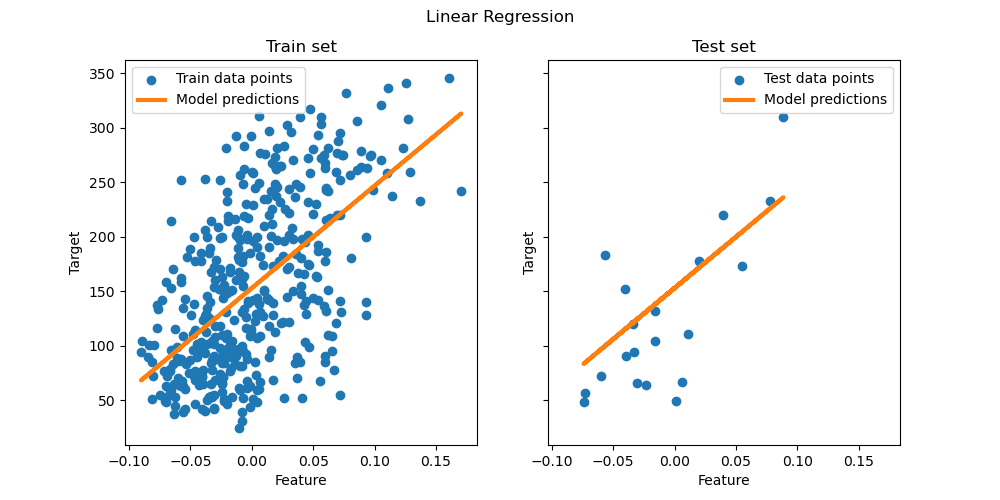
\includegraphics[width=0.75\linewidth]{Imagens/chap02/reg_OLS.png}
    \caption[Exemplo de regressão linear OLS]{Exemplo de regressão linear pelo método dos mínimos quadrados ordinários (OLS).}
    \fonte{\cite{sklearn_groupkfold_docs}}
    \label{fig:reg_ols}
\end{figure}

Os estimadores de mínimos quadrados dependem fortemente da independência linear entre as colunas da matriz de projeto \(\mathbf{X}\). Quando existe correlação elevada entre preditores — situação conhecida como multicolinearidade — a matriz \(\mathbf{X}^T \mathbf{X}\) pode tornar-se próxima de singular. Como consequência, a solução dos mínimos quadrados torna-se numericamente instável e altamente sensível a pequenas variações nos dados, produzindo estimativas com grande variância (\cite{scikit-learn-linear-model}). 

Esse fenômeno compromete a capacidade de generalização do modelo e motiva o uso de modelos lineares regularizados. Conforme discutido anteriormente, a regularização atua como um mecanismo de controle de complexidade, restringindo a flexibilidade do modelo e reduzindo sua sensibilidade às particularidades do conjunto de treinamento. Nesta seção, essa ideia é retomada no contexto específico dos modelos lineares, por meio das regressões Ridge e Lasso, apresentadas a seguir.

\subsubsection{Regressão Regularizada}

A regularização é uma técnica que penaliza a complexidade do modelo para melhorar sua capacidade de generalização e mitigar problemas como multicolinearidade ou sobreajuste (overfitting). Modelos regularizados adicionam termos de penalização à função de custo.

\paragraph{Ridge Regression (Penalização L2)}

A regressão Ridge surge como uma extensão da regressão linear ordinária com o objetivo de mitigar problemas associados à multicolinearidade e à elevada variância das estimativas. O método introduz uma penalização quadrática sobre os coeficientes do modelo, modificando o problema de otimização para

\begin{equation}
\hat{\mathbf{w}}
=
\arg\min_{\mathbf{w}}
\left(
\|\mathbf{X}\mathbf{w} - \mathbf{y}\|_2^2
+
\alpha \|\mathbf{w}\|_2^2
\right),
\end{equation}

onde \(\alpha \ge 0\) é o parâmetro de regularização.


\medskip

O termo adicional \(\alpha \|\mathbf{w}\|_2^2\) impõe uma penalização proporcional ao quadrado da magnitude dos coeficientes. À medida que \(\alpha\) aumenta, maior é o encolhimento (shrinkage) aplicado aos parâmetros do modelo, reduzindo sua magnitude e tornando a solução mais robusta à colinearidade entre variáveis explicativas.

O parâmetro \(\alpha\) controla diretamente o compromisso entre ajuste aos dados e complexidade do modelo. Para \(\alpha = 0\), recupera-se a solução de mínimos quadrados ordinários. Para valores crescentes de \(\alpha\), os coeficientes são progressivamente reduzidos em magnitude, o que diminui a variância do estimador, ainda que introduza um viés adicional.

Esse comportamento ilustra o clássico compromisso viés-variância: o aumento da regularização tende a reduzir a sensibilidade do modelo a flutuações nos dados de treinamento, melhorando potencialmente sua capacidade de generalização.

\paragraph{Lasso Regression (Penalização L1)}

A Lasso (Least Absolute Shrinkage and Selection Operator) é um modelo linear regularizado que introduz uma penalização baseada na norma L1 dos coeficientes. Diferentemente da Ridge regression, cuja penalização é quadrática, a Lasso impõe uma penalização linear sobre a magnitude absoluta dos parâmetros, favorecendo soluções esparsas.

O problema de otimização associado pode ser escrito como

\begin{equation}
\hat{\mathbf{w}}
=
\arg\min_{\mathbf{w}}
\left(
\frac{1}{2n}
\|\mathbf{X}\mathbf{w} - \mathbf{y}\|_2^2
+
\alpha \|\mathbf{w}\|_1
\right),
\end{equation}

onde
\(
\|\mathbf{w}\|_1 = \sum_{j=1}^{p} |w_j|
\)
e \(\alpha \ge 0\) controla a intensidade da regularização.

A principal característica da penalização \(L_1\) é sua capacidade de produzir coeficientes exatamente nulos. Como consequência, a Lasso pode realizar seleção implícita de variáveis, reduzindo o número efetivo de preditores utilizados pelo modelo.

Essa propriedade pode ser vantajosa quando há muitas variáveis candidatas ou quando se deseja obter um modelo mais simples e interpretável, pois variáveis com coeficientes nulos deixam de contribuir para a predição. No entanto, essa característica também deve ser interpretada com cuidado: em bases de dados pequenas ou com variáveis correlacionadas, a Lasso pode selecionar apenas uma entre variáveis com informações semelhantes, o que pode afetar a estabilidade da seleção.

Assim, Lasso é relevante não apenas como modelo de regressão regularizado, mas também como uma alternativa capaz de reduzir a complexidade do modelo por meio da exclusão automática de variáveis pouco informativas.

Assim como em outros modelos regularizados, o parâmetro \(\alpha\) controla o compromisso entre ajuste aos dados e complexidade do modelo. Valores elevados de \(\alpha\) aumentam a esparsidade e o viés do estimador, enquanto valores reduzidos aproximam a solução do estimador de mínimos quadrados ordinários.

\paragraph{Elastic Net}

O método Elastic Net combina as penalizações L1 e L2 em um único modelo linear regularizado. Seu objetivo é integrar a capacidade de seleção de variáveis da Lasso com a estabilidade numérica da Ridge, especialmente em cenários onde há correlação entre preditores.

O problema de otimização pode ser formulado como

\begin{equation}
\hat{\mathbf{w}}
=
\arg\min_{\mathbf{w}}
\left(
\frac{1}{2n}
\|\mathbf{X}\mathbf{w} - \mathbf{y}\|_2^2
+
\alpha
\left(
\rho \|\mathbf{w}\|_1
+
\frac{1-\rho}{2}
\|\mathbf{w}\|_2^2
\right)
\right),
\end{equation}

onde \(\alpha \ge 0\) controla a intensidade global da regularização e
\(\rho \in [0,1]\) determina o balanço entre as penalizações L1 e L2.

O parâmetro \(\rho\) define a combinação convexa entre as duas penalizações. Para \(\rho = 1\), o modelo reduz-se à Lasso; para \(\rho = 0\), torna-se equivalente à Ridge. Valores intermediários produzem um compromisso entre esparsidade e estabilidade.

O parâmetro \(\alpha\), por sua vez, controla o grau total de regularização aplicado ao modelo.

Em situações nas quais múltiplas variáveis apresentam forte correlação entre si, a Lasso tende a selecionar apenas uma delas, descartando as demais. O Elastic Net, ao incorporar o termo L2, tende a selecionar conjuntamente variáveis correlacionadas, distribuindo os coeficientes entre elas.

Essa propriedade torna o método particularmente útil em problemas com grupos de preditores correlacionados.

Outra vantagem prática do Elastic Net é sua maior estabilidade sob transformações lineares das variáveis de entrada. A presença da penalização L2 contribui para reduzir a sensibilidade da solução a pequenas perturbações nos dados, característica herdada da regressão Ridge.

Assim, o Elastic Net pode ser interpretado como uma generalização que engloba tanto a Lasso quanto a Ridge como casos particulares. Ele oferece maior flexibilidade na modelagem do compromisso entre viés, variância e esparsidade estrutural.


\subsubsection{Árvores de Decisão}

Árvores de Decisão (Decision Trees -- DTs) são métodos supervisionados não paramétricos utilizados para classificação e regressão. O objetivo é criar um modelo que prediga o valor de uma variável alvo por meio da aprendizagem de regras de decisão simples inferidas a partir dos atributos dos dados. Uma árvore pode ser vista como uma aproximação constante por partes.

Quanto maior a profundidade da árvore, mais complexas se tornam as regras de decisão e mais ajustado o modelo tende a ficar.

\begin{table}[H]
\centering
\caption[Vantagens e limitações das árvores de decisão]{Vantagens e limitações das árvores de decisão.}
\label{tab:vantagens_desvantagens_arvores}
\begin{tabular}{p{6.5cm} p{7.5cm}}
\hline
\textbf{Vantagens} & \textbf{Limitações} \\
\hline

São modelos de fácil interpretação, pois a estrutura da árvore permite visualizar as regras de decisão utilizadas para gerar as previsões. 
&
Podem apresentar \textit{overfitting} quando a árvore cresce excessivamente, ajustando-se a detalhes específicos do conjunto de treinamento e perdendo capacidade de generalização. \\

Exigem menor preparação prévia dos dados em comparação com outros métodos, pois não dependem diretamente de padronização das variáveis. 
&
São modelos instáveis, uma vez que pequenas alterações nos dados podem gerar árvores com estruturas bastante diferentes. \\

Podem capturar relações não lineares e interações entre variáveis sem a necessidade de especificar previamente a forma funcional da relação entre entradas e saída. 
&
Produzem previsões constantes por partes, o que pode limitar sua capacidade de representar relações suaves e comprometer sua aplicação em extrapolação. \\

Podem ser aplicadas tanto a problemas de classificação quanto de regressão, incluindo situações com múltiplas saídas, dependendo da implementação utilizada. 
&
A construção da árvore ótima é computacionalmente difícil; por isso, os algoritmos práticos utilizam estratégias heurísticas, que não garantem uma solução globalmente ótima. \\

Apresentam boa transparência em comparação com modelos do tipo \textit{black box}, como redes neurais, facilitando a análise das regras utilizadas pelo modelo. 
&
Podem apresentar viés quando há desbalanceamento nos dados ou quando determinadas regiões do espaço de entrada são pouco representadas. \\

\hline
\end{tabular}
\fonte{Adaptado de \cite{sklearn_groupkfold_docs}.}
\end{table}

A Figura~\ref{fig:arvore_decisao} ilustra o comportamento de uma árvore de decisão aplicada a um problema de regressão. Diferentemente de modelos lineares, que ajustam uma função contínua aos dados, a árvore de decisão aproxima a relação entre entrada e saída por regiões constantes por partes. A figura também permite observar o efeito da profundidade máxima da árvore sobre a complexidade do modelo: árvores mais rasas produzem aproximações mais simples, enquanto árvores mais profundas conseguem se ajustar mais detalhadamente aos dados.

\begin{figure}[H]
    \centering
    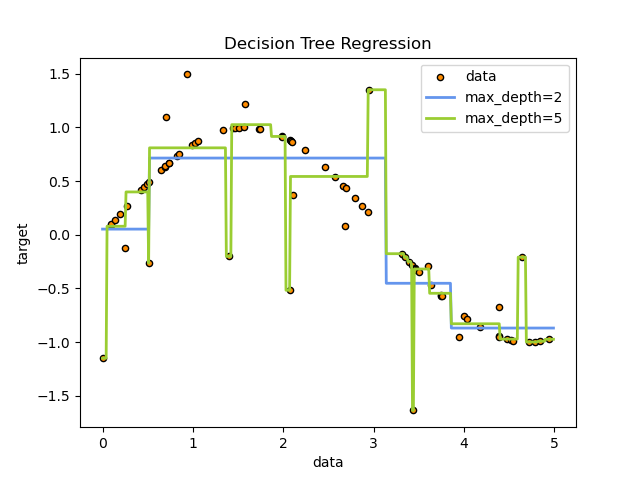
\includegraphics[width=0.5\linewidth]{Imagens/chap02/arvore.png}
    \caption[Regressão por árvore de decisão]{Exemplo de regressão utilizando árvore de decisão com diferentes profundidades, ilustrando o impacto da complexidade do modelo na capacidade de ajuste aos dados. Fonte: \cite{sklearn_groupkfold_docs}}
    \label{fig:arvore_decisao}
\end{figure}

Na Figura~\ref{fig:arvore_decisao}, a árvore com menor profundidade apresenta uma aproximação mais suave e simplificada da tendência geral dos dados. Já a árvore com maior profundidade acompanha variações mais locais, produzindo uma função mais irregular. Esse comportamento ilustra o compromisso entre flexibilidade e capacidade de generalização: o aumento da profundidade pode reduzir o erro no conjunto de treinamento, mas também aumenta o risco de \textit{overfitting}, caso o modelo passe a capturar flutuações específicas da amostra em vez do padrão geral dos dados.
\paragraph{Formulação Matemática}

Dados vetores de treinamento \(x_i \in \mathbb{R}^n\), \(i = 1, \dots, l\), e um vetor de rótulos \(y \in \mathbb{R}^l\), uma árvore de decisão particiona recursivamente o espaço de atributos de modo que amostras com os mesmos rótulos ou valores-alvo semelhantes sejam agrupadas.

Sejam os dados no nó \(m\) representados por \(Q_m\), contendo \(n_m\) amostras. Para cada divisão candidata \(\theta = (j, t_m)\), composta por um atributo \(j\) e um limiar \(t_m\), os dados são particionados em dois subconjuntos. O subconjunto à esquerda reúne as observações cujo valor do atributo \(j\) é menor ou igual ao limiar \(t_m\):

\begin{equation}
Q_m^{\mathrm{left}}(\theta) =
\{(x,y)\,|\, x_j \leq t_m\}.
\label{eq:subconjunto_esquerda_arvore}
\end{equation}

\noindent O subconjunto à direita é formado pelas demais observações do nó \(m\), isto é:

\begin{equation}
Q_m^{\mathrm{right}}(\theta) =
Q_m \setminus Q_m^{\mathrm{left}}(\theta).
\label{eq:subconjunto_direita_arvore}
\end{equation}

\noindent em que \(Q_m^{\mathrm{left}}(\theta)\) e \(Q_m^{\mathrm{right}}(\theta)\) representam, respectivamente, os subconjuntos resultantes da divisão à esquerda e à direita, \(x_j\) é o valor do atributo \(j\), \(t_m\) é o limiar de divisão no nó \(m\), e \(\setminus\) indica a diferença entre conjuntos.

A qualidade de uma divisão candidata no nó \(m\) é avaliada por meio de uma função de impureza ou função de perda \(H(\cdot)\), cuja escolha depende da tarefa considerada, como classificação ou regressão. Essa qualidade pode ser expressa por:

\begin{equation}
G(Q_m,\theta) =
\frac{n_m^{\mathrm{left}}}{n_m} H\left(Q_m^{\mathrm{left}}(\theta)\right)
+
\frac{n_m^{\mathrm{right}}}{n_m} H\left(Q_m^{\mathrm{right}}(\theta)\right).
\label{eq:criterio_divisao_arvore}
\end{equation}

\noindent em que \(G(Q_m,\theta)\) representa o valor do critério associado à divisão candidata \(\theta\) no nó \(m\), \(Q_m\) é o conjunto de amostras presentes nesse nó, \(n_m\) é o número total de amostras em \(Q_m\), \(Q_m^{\mathrm{left}}(\theta)\) e \(Q_m^{\mathrm{right}}(\theta)\) são os subconjuntos resultantes da divisão, e \(n_m^{\mathrm{left}}\) e \(n_m^{\mathrm{right}}\) representam o número de amostras em cada subconjunto. A função \(H(\cdot)\) mede a impureza ou erro associado a cada subconjunto.

A divisão ótima é então obtida pela escolha da divisão candidata que minimiza o critério \(G(Q_m,\theta)\):

\begin{equation}
\theta^* = \arg\min_{\theta} G(Q_m,\theta).
\label{eq:divisao_otima_arvore}
\end{equation}

\noindent em que \(\theta^*\) representa a melhor divisão encontrada para o nó \(m\), segundo o critério de impureza ou perda adotado.

A escolha da divisão em cada nó pode seguir diferentes estratégias. Uma estratégia baseada em busca exaustiva seleciona o par atributo--limiar que minimiza exatamente \(G(Q_m,\theta)\), avaliando todos os atributos disponíveis e todos os limiares possíveis. Alternativamente, pode-se utilizar uma estratégia aleatória, na qual um limiar candidato é amostrado aleatoriamente para cada atributo, resultando em uma aproximação estocástica da busca exaustiva e reduzindo o custo computacional.

Após selecionar a divisão ótima \(\theta^*\) no nó \(m\), o procedimento é aplicado recursivamente aos subconjuntos \(Q_m^{\mathrm{left}}(\theta^*)\) e \(Q_m^{\mathrm{right}}(\theta^*)\) até que uma condição de parada seja satisfeita, como profundidade máxima da árvore, número mínimo de amostras no nó ou redução mínima de impureza.

As árvores de decisão apresentam características que as tornam atrativas em problemas de regressão, especialmente pela facilidade de interpretação e pela capacidade de representar relações não lineares entre as variáveis. Entretanto, essas vantagens vêm acompanhadas de limitações importantes, principalmente relacionadas à instabilidade do modelo e ao risco de sobreajuste. A Tabela~\ref{tab:vantagens_desvantagens_arvores} resume os principais pontos positivos e negativos associados a esse tipo de modelo.
\subsubsection{Métodos de Combinação de Modelos (Ensemble Methods)}

Métodos de combinação de modelos (ensemble methods) consistem na estratégia de combinar as predições de múltiplos estimadores base, construídos a partir de um mesmo algoritmo de aprendizado, com o objetivo de melhorar a capacidade de generalização e a robustez do modelo final em comparação com um único estimador isolado.

Dois exemplos amplamente utilizados dessa abordagem são as Florestas Aleatórias (Random Forests) e o Gradient Boosting com Árvores de Decisão.

\subsubsection{Gradient Boosting com Árvores de Decisão}

O \textit{boosting} é um método de combinação de modelos no qual múltiplos estimadores simples, também chamados de \textit{weak learners}, são ajustados de forma sequencial para formar um modelo preditivo mais robusto. A ideia central é que cada novo estimador seja treinado buscando reduzir os erros remanescentes do modelo acumulado até a etapa anterior, de modo que a predição final resulte da combinação aditiva dos estimadores ajustados ao longo das iterações (\cite{Friedman2000}).

O \textit{Gradient Boosting} generaliza essa lógica ao formular o ajuste sequencial como uma descida do gradiente no espaço de funções. Nesse caso, a cada iteração, um novo estimador é ajustado na direção do gradiente negativo de uma função de perda diferenciável, permitindo aplicar o método a diferentes problemas supervisionados, incluindo regressão e classificação (\cite{Friedman2001}).


Modelos de \textit{Gradient Boosting} são modelos aditivos. A predição para uma entrada \(x_i\) é dada por:

Modelos de Gradient Boosting são modelos aditivos. A predição para uma entrada \( x_i \) é dada por

\[
\hat{y}_i = F_M(x_i) = \sum_{m=1}^{M} h_m(x_i),
\]

onde \( h_m \) são estimadores base, frequentemente chamados de \textit{weak learners} no contexto de boosting. No caso do Gradient Boosting com Árvores, esses estimadores base são árvores de decisão de tamanho fixo. O número total de árvores é denotado por \( M \).

O modelo é construído de forma sequencial e aditiva, por meio de um procedimento de otimização etapa a etapa, no qual cada novo estimador é ajustado para reduzir a função de perda considerando o modelo acumulado até a iteração anterior.

\[
F_m(x) = F_{m-1}(x) + h_m(x),
\]

onde cada nova árvore \( h_m \) é ajustada para minimizar uma função de perda acumulada:

\[
h_m = \arg\min_{h} \sum_{i=1}^{n} L\big(y_i, F_{m-1}(x_i) + h(x_i)\big),
\]

sendo  \(L(\cdot)\) uma função de perda diferenciável.

O modelo inicial \(F_0\) é escolhido como a constante que minimiza a função de perda antes da adição dos estimadores sequenciais. No caso da perda quadrática, tem-se:

\begin{equation}
F_0 = \arg\min_c \sum_{i=1}^{n} (y_i - c)^2.
\end{equation}

\noindent A solução desse problema é a média empírica dos valores alvo, isto é:

\begin{equation}
F_0 = \bar{y}.
\end{equation}

\noindent Assim, o modelo parte de uma predição inicial simples, correspondente à média dos valores observados, que é progressivamente corrigida pelos estimadores adicionados nas etapas seguintes.

Utilizando uma aproximação de Taylor de primeira ordem, pode-se demonstrar que, a cada iteração, a nova árvore \( h_m \) é ajustada para aproximar o gradiente negativo da função de perda em relação às predições atuais. Denotando

\[
g_i = \left[ \frac{\partial l(y_i, F(x_i))}{\partial F(x_i)} \right]_{F = F_{m-1}},
\]

a otimização se reduz, desprezando termos constantes, a

\[
h_m \approx \arg\min_{h} \sum_{i=1}^{n} h(x_i) g_i.
\]

Assim, a cada iteração, o estimador base é ajustado para prever o gradiente negativo da função de perda. Esse procedimento pode ser interpretado como uma forma de descida do gradiente em um espaço funcional.

\subsubsection{Controle da Complexidade das Árvores}

O tamanho das árvores de regressão utilizadas como estimadores base determina o nível de interação entre variáveis que o modelo pode capturar. Em geral, uma árvore de profundidade \( h \) pode capturar interações de ordem \( h \).

Existem duas formas principais de controlar o tamanho das árvores:

\begin{itemize}
\item Limitando a profundidade máxima da árvore, o que resulta em árvores binárias completas com até \( 2^h \) folhas e \( 2^h - 1 \) nós internos;
\item Limitando o número máximo de folhas, caso em que as árvores são construídas priorizando as divisões que produzem maior redução de impureza.
\end{itemize}

O controle do número de folhas define diretamente o grau máximo de interação modelável, sendo que uma árvore com \( k \) folhas possui \( k - 1 \) nós de divisão.

Em problemas com grande número de amostras, versões baseadas em histogramas podem apresentar ganhos significativos de eficiência computacional, além de oferecer suporte nativo a dados categóricos e valores ausentes. Em contrapartida, em conjuntos de dados pequenos, versões tradicionais podem ser preferíveis, pois a discretização por histogramas pode produzir pontos de divisão excessivamente aproximados.


\subsubsection{Random Forests e Outros Conjuntos de Árvores Aleatorizadas}

O conjunto de métodos de combinação de modelos (\textit{ensemble}) inclui algoritmos baseados na média de árvores de decisão aleatorizadas, como o \textit{Random Forest} e o método \textit{Extra-Trees}. Ambos seguem uma estratégia de perturbação e combinação ( do inglês, \textit{perturb-and-combine}), na qual diferentes árvores são construídas introduzindo variações nos dados de treinamento ou no processo de divisão dos nós. As previsões produzidas pelas árvores individuais são então combinadas, geralmente por meio de média, resultando em uma predição final mais robusta e menos sensível às particularidades de uma única árvore.

Assim como outros classificadores, modelos baseados em florestas são ajustados a partir de um conjunto de amostras de treinamento \(X \in \mathbb{R}^{n_{\text{samples}} \times n_{\text{features}}}\) e de um vetor de alvos \(Y \in \mathbb{R}^{n_{\text{samples}}}\). De forma análoga às árvores de decisão individuais, florestas também podem ser estendidas para problemas de múltiplas saídas.

\subsubsection{Random Forest}

Em Random Forests, cada árvore do conjunto é construída a partir de uma amostra obtida com reposição (\textit{bootstrap}) do conjunto de treinamento.

Durante a construção de cada árvore, um subconjunto aleatório das variáveis de entrada é considerado em cada divisão. O tamanho desse subconjunto pode incluir todas as variáveis ou apenas uma fração delas. 

Essas duas fontes de aleatoriedade — a amostragem com reposição das amostras e a seleção aleatória de variáveis em cada divisão — têm como objetivo reduzir a variância do estimador. Árvores de decisão individuais tendem a apresentar alta variância e, consequentemente, podem sofrer de sobreajuste. A aleatoriedade introduzida na floresta produz árvores com erros parcialmente desacoplados. Ao calcular a média das predições dessas árvores, parte desses erros pode se cancelar, reduzindo a variância global do modelo, possivelmente ao custo de um pequeno aumento no viés. Na prática, a redução de variância costuma ser significativa, resultando em melhor desempenho geral.

Durante o crescimento de cada árvore na floresta, a melhor divisão é escolhida de acordo com o critério de impureza, de maneira equivalente ao procedimento padrão utilizado em árvores de decisão do tipo CART. No caso de regressão, cada árvore produz uma previsão contínua para a variável de saída, e a previsão final da floresta é obtida pela média das previsões individuais. Essa combinação reduz a dependência em relação a uma única árvore e tende a diminuir a variância do modelo, tornando a predição mais robusta frente a pequenas variações no conjunto de treinamento.





\subsubsection{Perceptron Multicamadas (Multi-Layer Perceptron)}

O Perceptron Multicamadas (MLP) é um algoritmo de aprendizado supervisionado que aprende uma função 
\begin{equation}
f: \mathbb{R}^{m} \rightarrow \mathbb{R}^{o},
\label{eq:mlp_mapeamento}
\end{equation}
a partir de um conjunto de dados, onde \( m \) representa o número de dimensões de entrada e \( o \) o número de dimensões de saída. 

Dado um conjunto de atributos \( X = \{x_1, x_2, \dots, x_m\} \) e um alvo \( y \), o MLP é capaz de aprender um aproximador não linear da função de mapeamento, podendo ser aplicado tanto em problemas de classificação quanto de regressão. Diferentemente da regressão logística, o MLP possui uma ou mais camadas intermediárias não lineares entre a camada de entrada e a camada de saída, denominadas camadas ocultas.

A camada de entrada é composta por neurônios que representam diretamente os atributos de entrada. Cada neurônio em uma camada oculta realiza uma combinação linear ponderada das saídas da camada anterior,

\begin{equation}
w_1 x_1 + w_2 x_2 + \dots + w_m x_m
\end{equation}


seguida da aplicação de uma função de ativação não linear \( g(\cdot) : \mathbb{R} \rightarrow \mathbb{R} \), como, por exemplo, a tangente hiperbólica. A camada de saída recebe as ativações da última camada oculta e as transforma nos valores finais do modelo.

O modelo é parametrizado por matrizes de pesos que conectam camadas consecutivas e por vetores de bias associados a cada camada (exceto a camada de entrada). Cada matriz de pesos define as conexões entre duas camadas adjacentes, enquanto cada vetor de bias é somado às ativações lineares antes da aplicação da função de ativação.

\subsubsection{Algoritmos de Treinamento do MLP}

O MLP pode ser treinado utilizando diferentes algoritmos de otimização, como Gradiente Descendente Estocástico (SGD), Adam ou L-BFGS.

No caso do Gradiente Descendente Estocástico, os parâmetros são atualizados com base no gradiente da função de perda em relação aos pesos:

\[
w \leftarrow w - \eta \left[
\alpha \frac{\partial R(w)}{\partial w}
+
\frac{\partial \text{L}}{\partial w}
\right],
\]

onde \( \eta \) é a taxa de aprendizado, responsável por controlar o tamanho do passo na busca no espaço de parâmetros, \( \text{L} \) é a função de perda utilizada e \( R(w) \) representa um termo de regularização.

O método Adam também é um otimizador estocástico, porém ajusta automaticamente o tamanho das atualizações com base em estimativas adaptativas dos momentos de primeira e segunda ordem dos gradientes. Essa característica tende a favorecer a estabilidade do treinamento e a tornar o método menos sensível à escolha inicial da taxa de aprendizado.

Quando se utilizam métodos como SGD ou Adam, o treinamento pode ser realizado de forma \textit{online} ou por meio de mini-lotes. Isso permite atualizar os parâmetros a partir de subconjuntos dos dados, o que é vantajoso em bases maiores e em redes neurais treinadas iterativamente. Por outro lado, esses métodos podem exigir maior número de épocas e são sensíveis à escolha de hiperparâmetros, como taxa de aprendizado, tamanho do lote e critérios de parada.

O método L-BFGS, por sua vez, é um solucionador baseado em aproximações da matriz Hessiana, que representa as derivadas parciais de segunda ordem da função objetivo. Ele utiliza uma aproximação da inversa da Hessiana para atualizar os parâmetros, podendo apresentar convergência eficiente em problemas de menor dimensão ou com conjuntos de dados menores. Entretanto, diferentemente dos métodos baseados em gradiente estocástico, o L-BFGS não é adequado para aprendizado \textit{online} ou por mini-lotes, pois utiliza o conjunto de dados de forma mais global em cada atualização. Assim, sua aplicação pode se tornar menos prática em bases grandes, embora possa ser competitiva em problemas menores e bem condicionados.


\subsubsection{Vantagens e Limitações do MLP}

O Perceptron Multicamadas apresenta características que o tornam adequado para problemas de regressão não linear, como a capacidade de aproximar relações complexas entre variáveis de entrada e saída. Entretanto, essa flexibilidade também traz desafios relacionados ao treinamento, à escolha de hiperparâmetros e à sensibilidade ao pré-processamento dos dados. A Tabela~\ref{tab:vantagens_limitacoes_mlp} resume as principais vantagens e limitações associadas ao uso desse modelo.

\begin{table}[H]
\centering
\caption[Vantagens e limitações do Perceptron Multicamadas]{Vantagens e limitações do Perceptron Multicamadas.}
\label{tab:vantagens_limitacoes_mlp}
\begin{tabular}{p{6.5cm} p{7.5cm}}
\hline
\textbf{Vantagens} & \textbf{Limitações} \\
\hline

Capacidade de representar relações não lineares entre as variáveis de entrada e as saídas do modelo, o que torna o MLP adequado para problemas em que a relação entre as grandezas não pode ser descrita de forma simples ou linear.
&
A presença de camadas ocultas e funções de ativação não lineares torna a função de perda não convexa, podendo levar a diferentes soluções dependendo da inicialização dos pesos e do processo de treinamento. \\

Possibilidade de aprendizado incremental ou por mini-lotes, quando suportado pelo algoritmo de otimização utilizado, permitindo o ajuste iterativo dos parâmetros durante o treinamento.
&
O desempenho do modelo depende da escolha de diversos hiperparâmetros, como número de camadas ocultas, número de neurônios, função de ativação, taxa de aprendizado, regularização e critério de parada. \\

Capacidade de modelar interações complexas entre os atributos de entrada, sem exigir a especificação prévia da forma funcional da relação entre entradas e saídas.
&
O modelo é sensível à escala das variáveis de entrada, sendo recomendada a padronização prévia dos dados para evitar que diferenças de magnitude entre os atributos prejudiquem o treinamento. \\

\hline
\end{tabular}
\fonte{Adaptado de \cite{Sarkar2018PML}.}
\end{table}
\subsection{Modelos híbridos físico-informados e regularização baseada em física}
\label{sec:modelos-hibridos}

Em diversos problemas de engenharia, modelos puramente orientados a dados podem apresentar limitações importantes, especialmente em regimes com poucos dados rotulados e com forte estrutura física subjacente. Nesse contexto, abordagens híbridas buscam integrar conhecimento físico e aprendizado de máquina para induzir soluções mais plausíveis, consistentes e potencialmente mais robustas fora da distribuição de treinamento.

\subsubsection{Taxonomia de abordagens híbridas}
\label{subsec:taxonomia-hibrida}

Neste contexto, a taxonomia de abordagens híbridas refere-se a uma forma de classificar os diferentes modos pelos quais o conhecimento físico pode ser incorporado a modelos de aprendizado de máquina. Essa classificação é útil porque nem todas as abordagens híbridas combinam física e dados da mesma maneira: em alguns casos, a informação física é utilizada antes do treinamento, em outros é incorporada diretamente à estrutura do modelo e, em outros, aparece como restrição ou penalização na função de perda.

De acordo com \cite{rai2020hybrid}, as abordagens híbridas podem ser organizadas em três classes principais: (i) pré-processamento baseado em física, (ii) fusão na arquitetura do modelo de aprendizado de máquina e (iii) regularização baseada em física. A primeira classe abrange estratégias em que princípios físicos, modelos mecanísticos ou conhecimento externo são utilizados para transformar ou enriquecer as variáveis de entrada. A segunda classe refere-se a arquiteturas que incorporam explicitamente componentes físicos ou estruturais à rede. Já a terceira classe inclui métodos em que leis físicas, equações governantes ou relações conhecidas do sistema são incorporadas como restrições ou penalizações no processo de otimização, geralmente por meio de termos adicionais na função de perda.

A Figura~\ref{fig:taxonomia_hibrida_rai} apresenta essa classificação de forma esquemática. Nela, observa-se que o conhecimento físico pode ser incorporado em três momentos distintos do processo de modelagem. No primeiro caso, a física atua antes do treinamento, por meio do enriquecimento ou transformação das variáveis de entrada. No segundo, o conhecimento físico é incorporado à própria arquitetura do modelo, influenciando a forma como a rede neural processa as informações. No terceiro, a física é introduzida na função objetivo, penalizando soluções que se afastem de restrições, leis ou relações físicas conhecidas.

Essa representação é relevante para este trabalho porque permite situar as estratégias híbridas avaliadas posteriormente, especialmente aquelas em que a informação proveniente do modelo físico reduzido é utilizada como entrada adicional ou como termo de regularização durante o treinamento.

\begin{figure}[H]
    \centering
    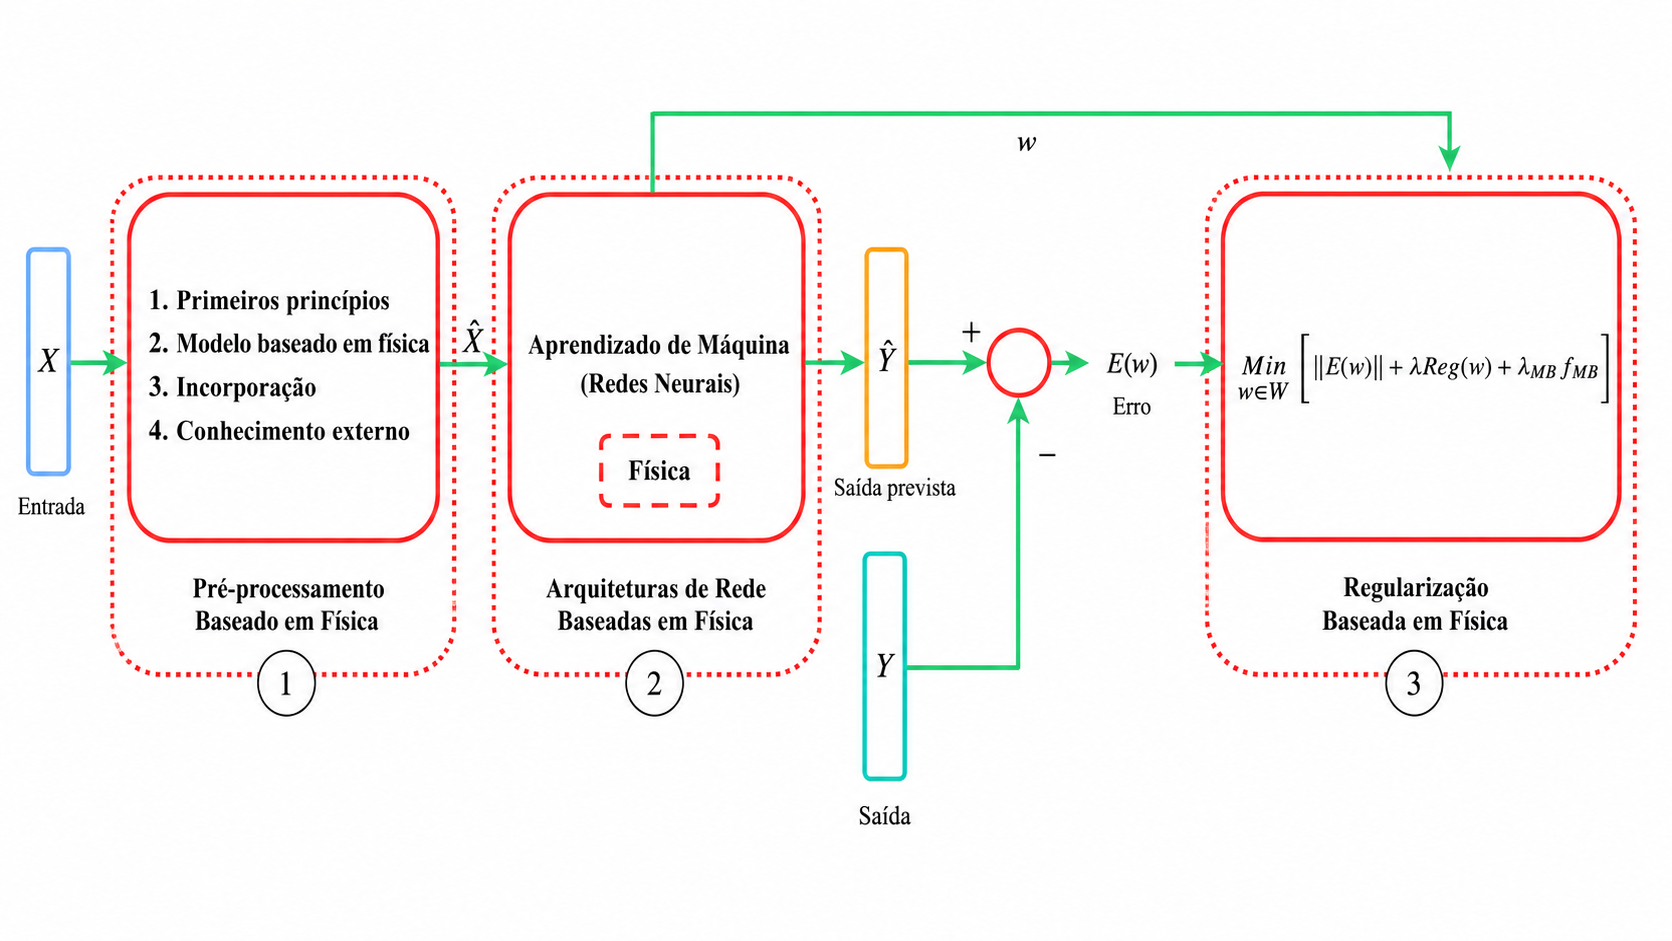
\includegraphics[width=0.95\linewidth]{Imagens/chap02/hybrid_tech.png}
    \caption[Taxonomia de abordagens híbridas guiadas por física]{Taxonomia de abordagens híbridas guiadas por física, classificadas em três categorias principais: (i) pré-processamento baseado em conhecimento físico, (ii) integração da física na arquitetura de redes neurais e (iii) incorporação de termos físicos na função de custo por meio de regularização.}
    \fonte{Adaptado de \cite{rai2020hybrid}.}
    \label{fig:taxonomia_hibrida_rai}
\end{figure}
\subsubsection{Regularização baseada em física via função de perda}

Uma formulação geral para tornar modelos de aprendizado de máquina mais consistentes com leis físicas consiste em acrescentar à função objetivo um termo adicional que penaliza violações de restrições físicas conhecidas do sistema. Nessa abordagem, a função de perda total passa a combinar três contribuições: (i) um termo de ajuste aos dados experimentais, que mede o erro entre valores observados e previstos; (ii) um termo de regularização clássica, associado ao controle da complexidade do modelo; e (iii) um termo de perda física, que quantifica o quanto as previsões do modelo desrespeitam leis físicas, equações governantes ou relações conhecidas do processo. De forma representativa, essa função pode ser escrita como \cite{willard2020}:

\begin{equation}
\mathcal{L} = \mathcal{L}_{\mathrm{TRN}}(\mathbf{Y}_{\mathrm{true}}, \mathbf{Y}_{\mathrm{pred}})
+ \lambda \,\mathcal{R}(\mathbf{W})
+ \gamma \,\mathcal{L}_{\mathrm{PHY}}(\mathbf{Y}_{\mathrm{pred}}),
\label{eq:loss_physics_based}
\end{equation}

\noindent em que $\mathcal{L}_{\mathrm{TRN}}(\mathbf{Y}_{\mathrm{true}}, \mathbf{Y}_{\mathrm{pred}})$ é o termo de ajuste aos dados de treinamento, normalmente definido por uma métrica de erro entre valores observados e previstos, como o erro quadrático médio; $\mathcal{R}(\mathbf{W})$ é o termo de regularização aplicado aos parâmetros do modelo $\mathbf{W}$, com o objetivo de controlar sua complexidade; e $\mathcal{L}_{\mathrm{PHY}}(\mathbf{Y}_{\mathrm{pred}})$ é o termo de perda física, responsável por penalizar previsões que violem relações físicas previamente conhecidas. Os parâmetros $\lambda$ e $\gamma$ controlam, respectivamente, a contribuição da regularização clássica e da restrição física na função objetivo total.

Do ponto de vista conceitual, a regularização física pode ser entendida como um mecanismo que restringe o conjunto de soluções admissíveis, impondo coerência com princípios físicos e reduzindo a dependência exclusiva de dados rotulados. Ao introduzir restrições físicas no processo de otimização, o espaço efetivo de busca para os parâmetros do modelo é reduzido, o que pode favorecer o aprendizado em regimes de poucos dados e incentivar previsões fisicamente consistentes.

É importante distinguir essa estratégia de uma \textit{Physics-Informed Neural Network} (PINN) em sentido estrito. Em uma PINN, as equações governantes do sistema, normalmente equações diferenciais ordinárias ou parciais, são incorporadas diretamente à função de perda por meio dos resíduos dessas equações. Assim, a rede é treinada não apenas para ajustar dados observados, mas também para satisfazer localmente as equações físicas no domínio considerado.

Na regularização física no nível da saída, por outro lado, a física não é necessariamente incorporada por meio do resíduo diferencial das equações governantes. Em vez disso, as previsões do modelo são comparadas com relações físicas conhecidas, restrições fenomenológicas ou saídas fornecidas por um modelo físico de referência. Dessa forma, o termo físico atua como uma penalização adicional sobre as saídas previstas, orientando o modelo a produzir respostas compatíveis com uma descrição física simplificada do sistema.


\subsubsection{Arquiteturas de redes baseadas em física}
\label{subsec:arquiteturas_fisicas}

Outra forma de integração entre conhecimento físico e modelos de
aprendizado de máquina consiste na incorporação explícita de
informações provenientes de modelos fenomenológicos na própria
arquitetura da rede neural. Nesse tipo de abordagem, o modelo físico
não atua apenas como uma fonte externa de informação, mas passa a
compor diretamente a estrutura do modelo híbrido.

De maneira geral, essa integração pode ocorrer de diferentes formas.
Uma possibilidade consiste em utilizar as predições de um modelo
físico como variáveis adicionais de entrada para a rede neural,
permitindo que o modelo baseado em dados explore diretamente a
informação fornecida pela modelagem fenomenológica. Alternativamente,
a rede neural pode ser estruturada para aprender o resíduo entre as
predições do modelo físico e os valores observados experimentalmente,
atuando como um mecanismo de correção sistemática das limitações do
modelo fenomenológico.

Essas estratégias caracterizam arquiteturas híbridas nas quais o
modelo físico e o modelo orientado a dados são acoplados de forma
estrutural. Nesse contexto, o modelo físico pode fornecer estimativas
iniciais, variáveis intermediárias ou componentes da própria função
de mapeamento aprendida pela rede neural, enquanto o modelo de
aprendizado de máquina captura efeitos não representados ou
aproximados na formulação física original.

Exemplos de arquiteturas desse tipo incluem modelos híbridos baseados
em dados físicos (\textit{hybrid physics data}), modelos de correção
residual e arquiteturas híbridas que combinam ambas as estratégias,
como discutido em \cite{zhou2025physics}. Em todos esses casos, o
modelo fenomenológico atua como parte integrante da arquitetura do
modelo híbrido, distinguindo essa classe de abordagens daquelas
baseadas apenas em regularização da função de perda.
\subsubsection{Relação com PINNs e perdas por resíduo de equações diferenciais}
\label{subsec:pinns}

Uma classe particularmente importante de métodos físico-informados são as \textit{Physics-Informed Neural Networks} (PINNs), nas quais a lei física é imposta via resíduo de uma equação diferencial. Nesse caso, a solução aproximada $u(t,x)$ é representada por uma rede neural, e o resíduo $f(t,x)$ associado à equação governante é também computado (por exemplo, via diferenciação automática). A função objetivo pode ser escrita como soma de um termo de ajuste a dados de contorno/iniciais e de um termo que impõe a estrutura física em pontos de colocalização \cite{raissi2019pinn}:
\begin{equation}
\label{eq:loss_pinn}
\mathrm{MSE}
=
\mathrm{MSE}_u + \mathrm{MSE}_f,
\end{equation}
onde $\mathrm{MSE}_u$ quantifica discrepâncias em relação aos dados observados (por exemplo, condições iniciais e de contorno) e $\mathrm{MSE}_f$ penaliza o resíduo físico (idealmente nulo) em um conjunto finito de pontos do domínio.

Essa construção formaliza a ideia de que conhecimento físico atua como uma forma de viés indutivo: ao impor estrutura adicional ao problema, o modelo é direcionado para soluções compatíveis com leis físicas, o que pode ser particularmente relevante em cenários com aquisição de dados limitada.

\subsubsection{Regularização física no nível de saída em modelos híbridos}
\label{subsec:regularizacao_saida}

Além das PINNs, é comum empregar regularização física no nível de saída, isto é, incorporar na perda um termo que mede a inconsistência entre a predição do modelo e uma relação física conhecida (ou um modelo físico reduzido) avaliada nas mesmas condições de operação. Um exemplo representativo é a formulação em que a perda total combina um termo supervisionado e um termo físico ponderados por um hiperparâmetro de mistura \cite{zhou2025physics}:
\begin{equation}
\label{eq:loss_hibrida_ponderada}
\mathcal{L}_{\mathrm{total}}
=
(1-\lambda)\,\mathcal{L}_{\mathrm{data}}
+
\lambda\,\mathcal{L}_{\mathrm{phy}},
\end{equation}
em que $\mathcal{L}_{\mathrm{data}}$ mede o erro de predição em relação aos dados experimentais e $\mathcal{L}_{\mathrm{phy}}$ penaliza violações de relações físicas incorporadas como restrições durante o treinamento. O hiperparâmetro $\lambda \in [0,1]$ controla o compromisso entre fidelidade aos dados e aderência às restrições físicas, permitindo ajustar o grau de influência do conhecimento físico na estimação do modelo.

Em termos práticos, essa estratégia tende a ser especialmente atraente quando existe um modelo físico (ainda que simplificado) capaz de fornecer relações qualitativas ou quantitativas úteis para regularizar a aprendizagem. Nessa situação, a função de perda híbrida pode restringir soluções fisicamente implausíveis, mantendo o treinamento ancorado tanto em observações experimentais quanto em consistência física.



    \chapter{Metodologia Proposta}
\label{chap4}


Este capítulo descreve a metodologia adotada para o desenvolvimento, avaliação e comparação dos modelos preditivos aplicados ao sistema de destilação por membranas estudado. A abordagem proposta integra etapas de preparação e estruturação dos dados experimentais, definição de estratégias de validação consistentes com a natureza dos dados, seleção e ajuste de modelos de diferentes níveis de complexidade e incorporação de informações provenientes de um modelo físico reduzido.

Inicialmente, são apresentados os procedimentos de organização do conjunto de dados, pré-processamento e engenharia de atributos, incluindo critérios baseados em fundamentos físicos para definição das variáveis de entrada. Em seguida, descrevem-se as estratégias de validação cruzada e os critérios adotados para estimação de desempenho e seleção de modelos, com ênfase no controle de sobreajuste e na consideração da incerteza associada às estimativas.

Posteriormente, é detalhada a estrutura computacional do \textit{pipeline} de modelagem, que será explicado em mais detalhes nas próximas seções, bem como as famílias de modelos avaliadas e os respectivos espaços de busca de hiperparâmetros. Por fim, são apresentadas as estratégias de integração entre o modelo físico e os modelos baseados em dados, estabelecendo o arcabouço metodológico que sustenta a análise comparativa desenvolvida neste trabalho.

\subsection{Síntese do pipeline metodológico}

\begin{figure}[H]
\centering
\resizebox{0.85\textwidth}{!}{%
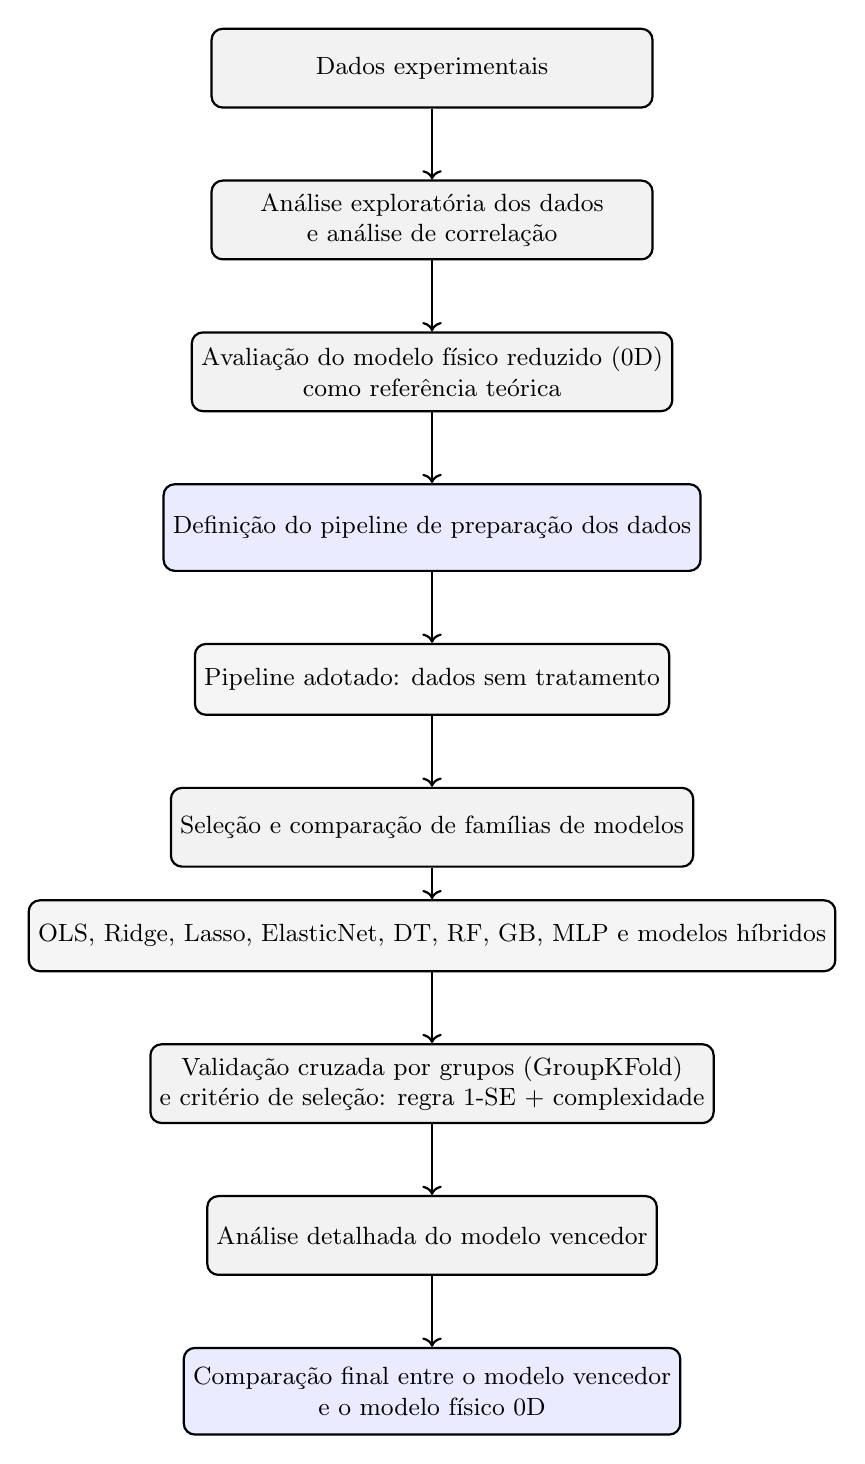
\begin{tikzpicture}[
    node distance=0.9cm,
    every node/.style={font=\small},
    block/.style={
        rectangle,
        rounded corners,
        draw=black,
        thick,
        align=center,
        minimum width=5.6cm,
        minimum height=1.0cm,
        fill=gray!10
    },
    decision/.style={
        rectangle,
        rounded corners,
        draw=black,
        thick,
        align=center,
        minimum width=6.2cm,
        minimum height=1.1cm,
        fill=blue!8
    },
    smallblock/.style={
        rectangle,
        rounded corners,
        draw=black,
        thick,
        align=center,
        minimum width=5.2cm,
        minimum height=0.9cm,
        fill=gray!8
    },
    arrow/.style={->, thick}
]

\node[block] (data)
{Dados experimentais};

\node[block, below=of data] (eda)
{Análise exploratória dos dados\\
e análise de correlação};

\node[block, below=of eda] (model0d)
{Avaliação do modelo físico reduzido (0D)\\
como referência teórica};

\node[decision, below=of model0d] (prep)
{Definição do pipeline de preparação dos dados};

\node[smallblock, below=of prep] (p1)
{Pipeline adotado: dados sem tratamento};

\node[block, below=of p1] (models)
{Seleção e comparação de famílias de modelos};

\node[smallblock, below=0.4cm of models] (families)
{OLS, Ridge, Lasso, ElasticNet, DT, RF, GB, MLP e modelos híbridos};

\node[block, below=of families] (cv)
{Validação cruzada por grupos (GroupKFold)\\
e critério de seleção: regra 1-SE + complexidade};

\node[block, below=of cv] (best)
{Análise detalhada do modelo vencedor};

\node[decision, below=of best] (final)
{Comparação final entre o modelo vencedor\\
e o modelo físico 0D};

\draw[arrow] (data) -- (eda);
\draw[arrow] (eda) -- (model0d);
\draw[arrow] (model0d) -- (prep);
\draw[arrow] (prep) -- (p1);
\draw[arrow] (p1) -- (models);
\draw[arrow] (models) -- (families);
\draw[arrow] (families) -- (cv);
\draw[arrow] (cv) -- (best);
\draw[arrow] (best) -- (final);

\end{tikzpicture}
}
\caption[Fluxograma do procedimento metodológico]{Fluxograma do procedimento metodológico adotado neste trabalho, desde a análise exploratória dos dados experimentais até a comparação final entre o modelo baseado em dados selecionado e o modelo físico reduzido (0D). O diagrama evidencia as principais etapas do estudo, incluindo a definição do procedimento de preparação dos dados, a avaliação de diferentes famílias de modelos e a seleção do modelo final com base em critérios de desempenho e parcimônia. Fonte: Autor.}
\label{fig:fluxograma_resultados_pipeline}
\end{figure}

\section{Estrutura do Sistema e Preparação dos Dados}
\label{sec:estrutura_sistema_dados}

Antes da construção dos modelos preditivos, é necessário delimitar o sistema físico que se deseja representar. Neste trabalho, considera-se um sistema de destilação por membranas na configuração \textit{Vacuum-Enhanced Air Gap Membrane Distillation} (V-AGMD), operado em escala piloto. O sistema utiliza um módulo espiralado, no qual a solução salina aquecida escoa pelos canais de alimentação, separados dos espaços de ar por membranas hidrofóbicas. Do outro lado do espaço de ar, placas de resfriamento atuam como superfícies de condensação, sendo mantidas frias pela circulação de água nos canais de resfriamento. A unidade também inclui um sistema de vácuo, responsável por induzir pressão reduzida no tanque de permeado e nos espaços de ar, além de um tanque para coleta do destilado (\cite{Lisboa2024}).

O funcionamento do processo está associado à diferença de temperatura entre a alimentação aquecida e a região fria de condensação. Essa diferença estabelece um gradiente de pressão parcial de vapor que promove a evaporação da água na interface entre a solução salina e a membrana. O vapor formado atravessa os poros da membrana hidrofóbica, enquanto os sais dissolvidos são retidos na alimentação. Em seguida, o vapor percorre o espaço de ar sob pressão reduzida e se difunde em direção à superfície fria de condensação, onde condensa e é coletado como permeado. A presença do espaço de ar contribui para reduzir perdas térmicas por condução, enquanto a operação sob vácuo reduz a resistência ao transporte de massa no domínio gasoso, favorecendo o aumento do fluxo de permeado (\cite{Lisboa2024}).

Do ponto de vista físico, o desempenho do sistema é governado pelo acoplamento entre transferência de massa e transferência de calor. A transferência de massa envolve o transporte de vapor através da membrana hidrofóbica e do espaço de ar, enquanto a transferência de calor inclui a convecção nas correntes líquidas, a condução através da membrana e do espaço de ar e o transporte de calor latente associado ao vapor. Dessa forma, alterações nas condições operacionais, como temperaturas de entrada, vazão, pressão de vácuo e salinidade, afetam diretamente a produtividade do processo e o comportamento térmico do módulo.

No presente trabalho, o sistema físico é representado por meio de variáveis operacionais de entrada e variáveis de desempenho de saída. As variáveis de entrada consideradas são a temperatura de entrada da alimentação, a temperatura de entrada da corrente de resfriamento, a vazão de entrada da corrente de resfriamento, a pressão de vácuo e a concentração de NaCl. Essas variáveis estão associadas à força motriz térmica do processo, ao regime de escoamento e tempo de residência das correntes, à resistência difusiva no espaço de ar e às propriedades termofísicas da solução salina. As variáveis de saída são o fluxo de permeado e as temperaturas de saída das correntes de alimentação e resfriamento.

A escolha dessas saídas está relacionada aos principais parâmetros de desempenho do sistema. O fluxo de permeado representa a produtividade do processo da destilação e, por isso, constitui a variável de maior interesse operacional neste trabalho. As temperaturas de saída, por sua vez, permitem avaliar o comportamento térmico do módulo e são relevantes para análises energéticas posteriores, incluindo a estimativa de indicadores como o consumo específico de energia térmica e a razão de ganho de saída. Dessa forma, os modelos avaliados neste trabalho buscam aprender a relação entre as condições operacionais impostas ao sistema V-AGMD e as respostas associadas tanto à produção de permeado quanto ao desempenho térmico do módulo.

\subsubsection{Estruturação do Conjunto de Dados}

O conjunto de dados utilizado neste trabalho é composto por observações experimentais associadas à operação de um sistema V-AGMD em escala piloto. Neste contexto, cada observação, ou ponto experimental, corresponde a uma linha da base de dados e representa uma condição específica de operação do módulo. Essa condição é definida pela combinação dos valores impostos às variáveis controladas experimentalmente: temperatura de entrada da alimentação, temperatura de entrada da corrente de resfriamento, vazão da corrente de resfriamento, pressão de vácuo no espaço de ar e concentração de NaCl. Essas variáveis descrevem as condições sob as quais o processo foi conduzido e estão diretamente relacionadas à força motriz térmica, ao regime de escoamento, à resistência difusiva no espaço de ar e às propriedades da solução salina (\cite{Lisboa2024}).

Para cada ponto experimental, foram registradas ou calculadas as respostas do sistema, isto é, as variáveis que caracterizam o desempenho do módulo naquela condição de operação. No contexto deste trabalho, as saídas consideradas são o fluxo de permeado e as temperaturas de saída das correntes de alimentação e de resfriamento. O fluxo de permeado representa a produtividade do processo, enquanto as temperaturas de saída permitem avaliar o comportamento térmico do módulo e servem como base para análises energéticas posteriores.

Dessa forma, a base de dados pode ser interpretada como uma tabela experimental estruturada para modelagem preditiva: cada linha corresponde a uma condição operacional testada no sistema V-AGMD, enquanto as colunas representam, de um lado, as variáveis de entrada controladas no experimento e, de outro, as respostas medidas ou calculadas para essa mesma condição.

Formalmente, o problema é estruturado como uma tarefa de regressão supervisionada de múltiplas saídas. Seja
\[
X \in \mathbb{R}^{n \times p}
\]
a matriz de variáveis de entrada, onde \( n \) representa o número total de observações experimentais e \( p \) o número de variáveis operacionais consideradas. Cada linha de \( X \) corresponde a um vetor de condições de operação do sistema.

As variáveis de saída são organizadas na matriz
\begin{equation}
Y \in \mathbb{R}^{n \times 3}    
\end{equation}

\noindent em que \(n\) representa o número total de observações experimentais e o número \(3\) corresponde às três variáveis de saída consideradas na modelagem.

cujas colunas representam, respectivamente, as temperaturas de saída do canal quente, as temperaturas de saída do canal frio e o fluxo de permeado. Dessa forma, cada observação experimental está associada simultaneamente a três grandezas de interesse, caracterizando o problema como regressão de multiplas saídas.

Além das matrizes \(X\) e \(Y\), a base de dados contém a variável denominada \textit{Regime}. Neste trabalho, o termo \textit{Regime} refere-se a um agrupamento de observações experimentais obtidas sob condições operacionais equivalentes ou próximas. Assim, amostras pertencentes ao mesmo regime compartilham características comuns do ensaio e, por isso, não devem ser tratadas como completamente independentes durante a avaliação dos modelos.

A variável \textit{Regime} é mantida separadamente das matrizes \(X\) e \(Y\), sendo utilizada exclusivamente para fins de agrupamento no processo de validação cruzada. Essa escolha permite preservar a estrutura dependente dos dados durante a etapa de avaliação de desempenho.

Essa organização formal estabelece a base para as etapas subsequentes de pré-processamento, validação e seleção de modelos.

\begin{figure}[H]
    \centering
    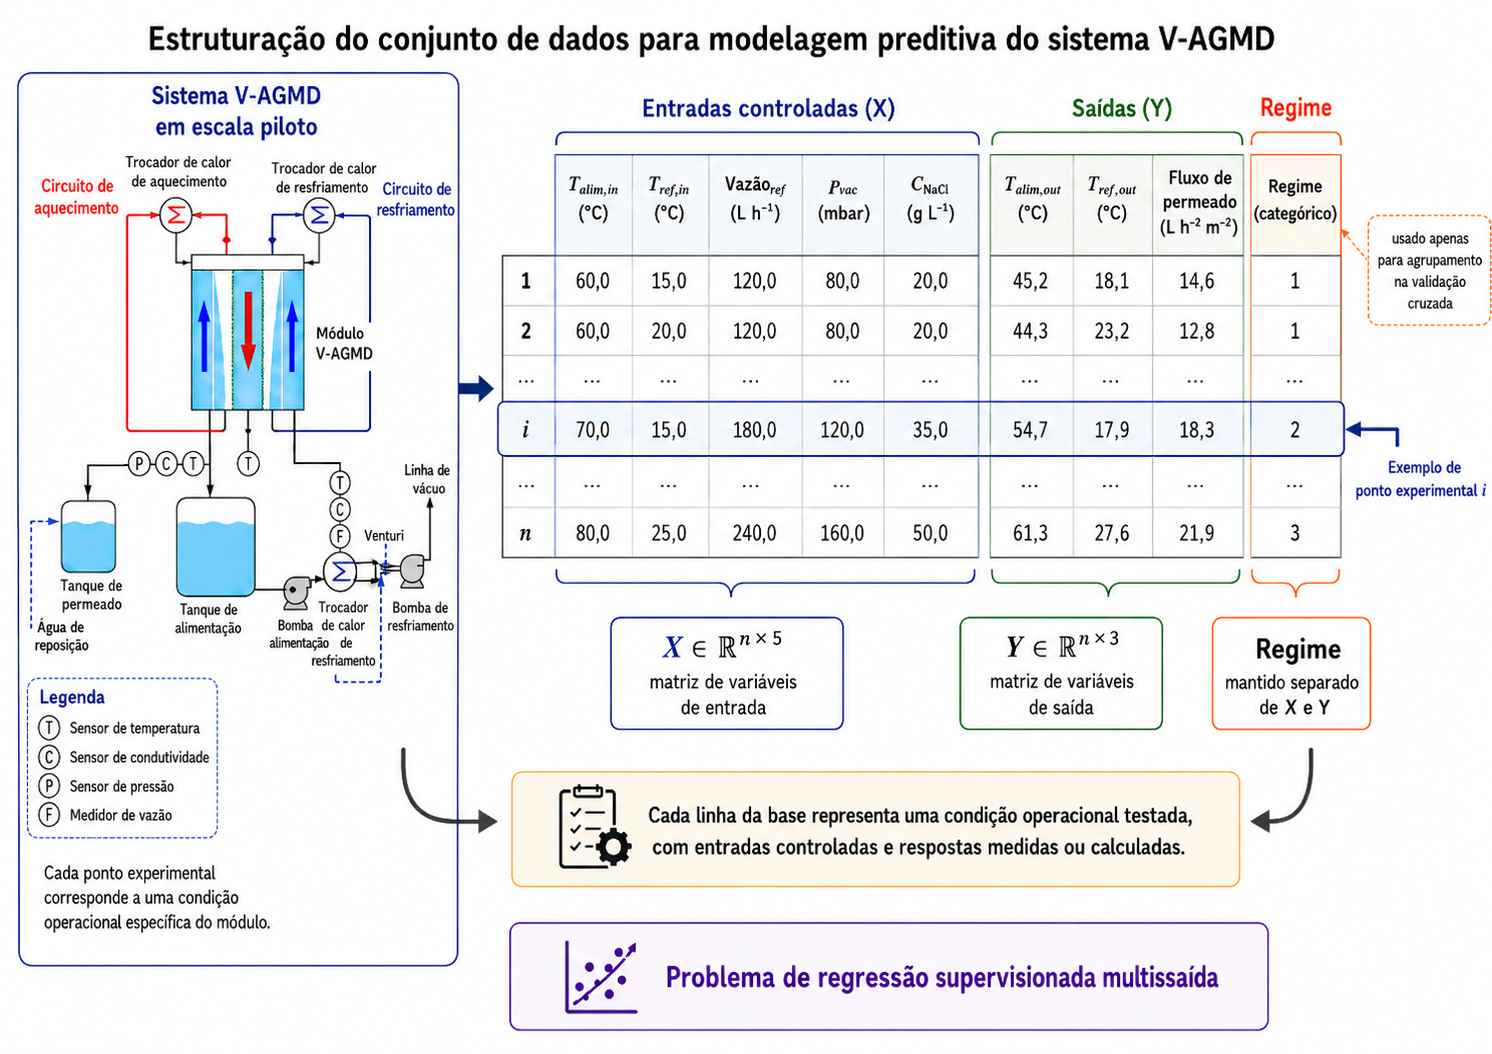
\includegraphics[width=1\linewidth]{Imagens/chap04/esquematizacao_regressao.png}
    \caption[Esquematização da estrutura do conjunto de dados para modelagem preditiva]{Esquematização da estrutura do conjunto de dados utilizado na modelagem preditiva do sistema V-AGMD. Cada linha da base representa um ponto experimental, definido por uma condição operacional específica do módulo. As variáveis de entrada são organizadas na matriz \(X \in \mathbb{R}^{n \times 5}\), enquanto as três variáveis de saída são organizadas na matriz \(Y \in \mathbb{R}^{n \times 3}\). A variável \textit{Regime} é mantida separadamente das matrizes \(X\) e \(Y\), sendo utilizada apenas para o agrupamento das observações na validação cruzada. Fonte: Elaborado pela autora com base em \cite{Lisboa2024}.}
    \label{fig:esquematizacao_regressao}
\end{figure}

\subsubsection{Tratamento da Variável de Agrupamento}

Como definido na seção anterior, a variável \textit{Regime} identifica grupos de observações experimentais associadas a condições operacionais equivalentes ou próximas. Essa variável não é utilizada como entrada dos modelos, mas apenas como informação auxiliar para orientar a divisão dos dados durante a validação cruzada.

A variável \textit{Regime} foi utilizada exclusivamente como identificador de agrupamento durante o processo de validação cruzada. Ela não foi incluída como variável de entrada nos modelos preditivos, a fim de evitar que o algoritmo explorasse informações implícitas sobre a estrutura experimental que não estariam disponíveis em cenários de generalização para novos regimes.

Essa decisão metodológica tem como objetivo preservar a coerência experimental do processo de avaliação. Caso observações pertencentes ao mesmo regime fossem distribuídas simultaneamente entre conjuntos de treinamento e validação, o modelo poderia se beneficiar de informações correlacionadas, produzindo estimativas excessivamente otimistas de desempenho.

Dessa forma, o particionamento dos dados foi conduzido respeitando os agrupamentos definidos pela variável \textit{Regime}, garantindo que todas as observações associadas a um mesmo regime fossem alocadas integralmente em um único subconjunto durante cada iteração da validação cruzada. Essa estratégia permite avaliar a capacidade dos modelos de generalizar para condições operacionais não previamente observadas.

\subsection{Estratégia de Escalonamento Adotada}

Neste trabalho, optou-se pela padronização das variáveis de entrada por meio da transformação para média zero e variância unitária, conforme definido pela Equação~\ref{eq:padronizacao_zscore}. Essa transformação corresponde ao procedimento implementado pelo \texttt{StandardScaler}, no qual cada variável é centralizada pela sua média e escalada pelo seu desvio padrão.

A escolha da padronização foi motivada pela presença de modelos lineares regularizados e redes neurais no conjunto de famílias avaliadas, ambos sensíveis à escala relativa das variáveis. Como este estudo tem como objetivo comparar diferentes classes de modelos sob um protocolo unificado de treinamento, validação e seleção, adotou-se uma única estratégia de escalonamento aplicável de forma consistente a todas as famílias. Dessa forma, reduz-se a influência arbitrária das unidades de medida sobre o desempenho dos modelos e torna-se mais justa a comparação entre abordagens distintas.


A transformação foi implementada por meio de um \textit{Pipeline}, isto é, uma sequência encadeada de etapas de pré-processamento e modelagem executadas de forma integrada. Nesse procedimento, o escalonamento não é aplicado previamente à base completa, mas sim incorporado ao fluxo de treinamento de cada modelo. Assim, em cada iteração da validação cruzada, o \texttt{StandardScaler} foi ajustado exclusivamente com os dados do subconjunto de treinamento, calculando a média e o desvio padrão apenas a partir dessas amostras. Em seguida, os mesmos parâmetros de padronização foram aplicados ao subconjunto de validação correspondente. Dessa forma, evitou-se o uso de estatísticas globais calculadas com o conjunto completo de dados, prevenindo vazamento de informação entre treino e validação.

Esse procedimento implica que cada partição da validação cruzada possui seus próprios parâmetros de padronização, definidos a partir do respectivo conjunto de treinamento. Entretanto, isso não compromete a comparação entre os modelos, pois todos os modelos avaliados em uma mesma partição são submetidos ao mesmo procedimento de escalonamento. Além disso, essa estratégia reproduz de forma mais adequada uma situação de generalização, na qual os parâmetros de pré-processamento devem ser estimados apenas com os dados disponíveis no treinamento e posteriormente aplicados a novas observações.

Técnicas alternativas, como normalização Min-Max e escalonamento robusto, não foram adotadas, uma vez que não se observou presença significativa de outliers extremos no conjunto de dados experimental, e a padronização mostrou-se adequada ao comportamento estatístico das variáveis analisadas.
\subsection{Encapsulamento em \textit{Pipeline} e Prevenção de Vazamento de Informação}

Todas as etapas de pré-processamento e modelagem foram encapsuladas por meio da utilização de objetos \textit{Pipeline}. Essa abordagem permite integrar, em uma única estrutura, a transformação das variáveis de entrada e o ajuste do modelo preditivo, garantindo consistência no fluxo computacional.

Em cada iteração da validação cruzada, os parâmetros associados às transformações (como média e desvio padrão da padronização) foram estimados exclusivamente a partir dos dados de treinamento do respectivo \textit{partição}. O subconjunto de validação foi transformado utilizando apenas essas estatísticas previamente ajustadas, sem acesso às informações globais do conjunto completo.

Essa estratégia é fundamental para evitar vazamento de informação (\textit{data leakage}), fenômeno que ocorre quando dados do conjunto de validação influenciam indiretamente o processo de treinamento, resultando em estimativas excessivamente otimistas de desempenho.

Adicionalmente, o procedimento de validação cruzada com agrupamento por regime foi integrado ao processo de busca de hiperparâmetros, assegurando que todas as transformações e ajustes fossem realizados respeitando a estrutura experimental dos dados. Dessa forma, tanto o pré-processamento quanto o treinamento foram conduzidos de maneira consistente e reprodutível ao longo de todas as famílias de modelos avaliadas.


\subsection{Estratégias de Engenharia de Atributos}

\subsubsection{Critérios para Seleção de Variáveis}

A definição do conjunto de variáveis de entrada foi conduzida a partir de critérios físicos e experimentais, priorizando apenas grandezas efetivamente impostas ao sistema antes da operação. Variáveis dependentes do comportamento interno do módulo — tais como temperaturas de saída, fluxo de permeado ou grandezas derivadas dessas quantidades — não foram consideradas elegíveis como preditores, pois representam respostas do sistema e não condições operacionais previamente conhecidas. Essa escolha evita que o modelo utilize, durante o treinamento, informações que não estariam disponíveis no momento da predição, preservando a coerência causal da modelagem.


Com o objetivo de manter a rastreabilidade entre a formulação física apresentada na Fundamentação Teórica e a implementação computacional dos modelos, adotou-se, na metodologia, a nomenclatura utilizada na base de dados e no código. Entretanto, como a Fundamentação Teórica emprega uma notação mais próxima da modelagem fenomenológica, baseada nos canais quente e frio do módulo, a Tabela~\ref{tab:relacao_variaveis_teoria_codigo} apresenta a correspondência entre os símbolos físicos discutidos anteriormente e os nomes das variáveis utilizados na etapa computacional.

\begin{table}[H]
\centering
\caption[Correspondência entre nomenclaturas das variáveis]{Correspondência entre a nomenclatura utilizada na Fundamentação Teórica e a nomenclatura adotada na base de dados e no código computacional.}
\label{tab:relacao_variaveis_teoria_codigo}
\begin{tabular}{p{5.2cm} p{4.2cm} p{3.2cm}}
\hline
\textbf{Nomenclatura na teoria} & \textbf{Nome no código/base} & \textbf{Uso no modelo} \\
\hline

\(T_f\), \(T_{f,in}\) ou temperatura da corrente quente
&
\texttt{Alim\_T\_in}
&
Entrada \\

\(T_c\), \(T_{c,in}\) ou temperatura da corrente fria
&
\texttt{Ref\_T\_in}
&
Entrada \\

\(\dot{V}_c\), \(\dot{m}_c\) ou vazão da corrente fria
&
\texttt{Ref\_V\_in}
&
Entrada \\

\(p\), \(p_{vac}\) ou pressão no espaço de ar
&
\texttt{P\_vacuum}
&
Entrada \\

\(C_{NaCl}\), \(x_{salt}\) ou salinidade
&
\texttt{C\_NaCl}
&
Entrada \\

\(j_w\)
&
\texttt{Flux}
&
Saída \\

\(T_{f,out}\)
&
\texttt{Alim\_T\_out}
&
Saída \\

\(T_{c,out}\)
&
\texttt{Ref\_T\_out}
&
Saída \\

\textit{Regime}
&
\texttt{Regime}
&
Agrupamento na validação cruzada \\

\hline
\end{tabular}
\end{table}

Todas as demais variáveis disponíveis no conjunto de dados foram excluídas por representarem saídas diretas do processo, grandezas derivadas ou variáveis internas calculadas a partir do balanço energético e de massa.

A partir desse conjunto elegível de cinco preditores, foi realizada uma busca exaustiva por subconjuntos (\textit{Best Subset Selection}), avaliando todas as combinações de tamanho $k = 3, 4, 5$. Cada subconjunto foi testado utilizando regressão linear multialvo, com validação cruzada baseada em \textit{GroupKFold}, respeitando a separação entre regimes experimentais.

Os resultados, que se encontram no Apendice A, evidenciaram melhoria monotônica do desempenho à medida que se aumentou o número de preditores. Para todas as variáveis de saída analisadas (\textit{Flux}, \textit{Alim\_T\_out} e \textit{Ref\_T\_out}), observou-se redução consistente do RMSE e aumento sistemático do coeficiente de determinação $R^2$ ao passar de $k=3$ para $k=4$ e de $k=4$ para $k=5$. Não foram identificados \textit{trade-offs} entre as saídas.

O subconjunto composto pelas cinco variáveis elegíveis apresentou simultaneamente os menores erros e os maiores valores de \(R^2\) para todos os alvos, superando os subconjuntos reduzidos avaliados. Esse resultado não altera a escolha física inicial das variáveis, mas fornece uma verificação empírica de que a remoção de qualquer uma das grandezas consideradas comprometeria o desempenho preditivo do modelo. Assim, a análise de subconjuntos funcionou como uma etapa de confirmação metodológica, indicando que não havia ganho em simplificar o conjunto de entradas previamente definido com base na fenomenologia do processo.

Além da superioridade estatística, a manutenção das cinco variáveis também é coerente do ponto de vista físico, pois elas contemplam grandezas operacionais que influenciam diretamente os fenômenos de transporte de calor e massa no sistema. As temperaturas de entrada definem a força motriz térmica, a vazão afeta o regime de escoamento e o tempo de residência, a pressão de vácuo modifica a resistência ao transporte de vapor e a concentração salina altera a pressão de vapor da solução.

Dessa forma, adotou-se como conjunto final de preditores:
\[
\{\text{Ref\_T\_in},\; \text{Alim\_T\_in},\; \text{V\_in},\; \text{P\_vacuum},\; \text{C\_NaCl}\}.
\]


\subsubsection{Avaliação do Uso de Discretização}

Nesta etapa, foi realizada uma análise exploratória para avaliar se a discretização das variáveis contínuas de entrada poderia contribuir para a modelagem preditiva do sistema V-AGMD. O objetivo não foi redefinir as variáveis de desempenho do sistema, mas verificar se os preditores previamente selecionados com base na fenomenologia do processo deveriam ser mantidos em sua forma contínua ou se alguma representação discretizada poderia favorecer o desempenho dos modelos.

As variáveis de saída permaneceram fixas ao longo de toda a análise, correspondendo ao fluxo de permeado e às temperaturas de saída das correntes de alimentação e de resfriamento. Portanto, as configurações comparadas nesta etapa referem-se apenas a diferentes representações das variáveis de entrada, e não a diferentes conjuntos de parâmetros de desempenho.

A motivação para essa avaliação está relacionada à possibilidade de que algumas variáveis operacionais apresentem padrões não lineares, regiões multimodais ou faixas de operação com comportamentos distintos. Nesses casos, a discretização poderia, em princípio, permitir que o modelo representasse melhor mudanças de comportamento associadas a determinados intervalos das variáveis de entrada. Por outro lado, essa transformação também pode reduzir a resolução das grandezas físicas originais, uma vez que substitui valores contínuos por categorias ou faixas discretas.

Foram consideradas as cinco variáveis de entrada elegíveis para a modelagem: temperatura de entrada da alimentação, temperatura de entrada da corrente de resfriamento, vazão de entrada da corrente de resfriamento, pressão de vácuo e concentração de NaCl. Para cada uma dessas variáveis, foram avaliadas duas possibilidades: manter a variável em sua forma contínua ou substituí-la por uma versão discretizada. A discretização foi realizada por meio de um modelo de mistura Gaussiana unidimensional, cujo número de componentes foi previamente definido com base nos critérios de informação AIC e BIC.

Dessa forma, como cada uma das cinco variáveis poderia assumir dois estados, contínua ou discretizada, foram avaliadas \(2^5 = 32\) configurações distintas de entrada. Cada configuração correspondeu, portanto, a uma combinação específica de variáveis contínuas e variáveis discretizadas utilizada como conjunto de preditores do modelo.

Para comparar essas configurações, foram treinados modelos de regressão linear multialvo, utilizando validação cruzada com \textit{GroupKFold}. A variável \textit{Regime} foi utilizada apenas como identificador de agrupamento na validação cruzada, preservando a estrutura dependente dos dados experimentais. O desempenho de cada configuração foi avaliado por meio das métricas RMSE e \(R^2\), calculadas para as três variáveis de saída. Os resultados detalhados desse estudo comparativo são apresentados no Apêndice~A.

Os resultados indicaram que algumas combinações específicas envolvendo discretização apresentaram melhora pontual para determinados alvos. No entanto, essas melhorias não foram consistentes de forma simultânea para as três variáveis de saída. Em particular, a configuração em que todas as variáveis de entrada foram mantidas em sua forma contínua apresentou desempenho competitivo ou superior na maioria dos cenários avaliados.

Assim, a análise não teve como principal contribuição identificar novas variáveis relevantes, uma vez que a seleção inicial dos preditores já havia sido fundamentada na descrição física do processo. Sua contribuição foi verificar empiricamente se a discretização ou a remoção da natureza contínua de alguma variável poderia simplificar a representação do problema sem perda de desempenho preditivo. Como esse ganho não foi observado de forma robusta, optou-se por preservar a forma contínua das grandezas físicas originais.

Diante da ausência de melhoria consistente e da importância de manter a interpretação fenomenológica das variáveis operacionais, estratégias de \textit{binning} não foram adotadas nas etapas subsequentes de modelagem. Assim, todas as variáveis de entrada foram mantidas em sua forma contínua ao longo do restante do estudo.

\section{Geração de variáveis físicas auxiliares}
\label{subsec:geracao_variaveis_phy}

O modelo físico 0D utilizado neste trabalho corresponde ao código em linguagem C desenvolvido no trabalho de \cite{Lisboa2024}. Nesta metodologia, não foi realizada uma nova implementação do modelo físico em Python. Em vez disso, foi elaborado um script auxiliar em Python para automatizar a execução do código em C para cada linha da base experimental.

Nesse procedimento, cada observação experimental foi lida pelo script em Python, que extraíu as variáveis operacionais correspondentes e as converteu para as unidades exigidas pelo executável do modelo físico. Em seguida, o código em C foi chamado automaticamente para calcular as estimativas físicas associadas àquela condição operacional, como o fluxo de permeado previsto pelo modelo 0D. Os resultados retornados pelo executável foram então armazenados e organizados na base de dados para uso posterior nas etapas de comparação e modelagem híbrida.

Durante esse processo, foram realizadas as conversões de unidades necessárias para compatibilizar a base experimental com as entradas esperadas pelo modelo físico, incluindo a conversão da pressão de vácuo de mbar para Pa, da vazão volumétrica de L/h para kg/s e da concentração salina para a unidade adotada na formulação do modelo.

Para cada observação experimental disponível, o modelo 0D foi executado utilizando como entradas as variáveis operacionais medidas no sistema: temperatura de entrada da corrente de alimentação (\texttt{Alim\_T\_in}), temperatura de entrada da corrente de resfriamento (\texttt{Ref\_T\_in}), vazão volumétrica da corrente de referência (\texttt{Ref\_V\_in}), pressão de vácuo no módulo (\texttt{P\_vacuum}) e concentração de NaCl na alimentação (\texttt{C\_NaCl}). Essas grandezas correspondem às variáveis experimentais disponíveis na base de dados utilizada neste trabalho.

O procedimento foi implementado por meio de um script em \texttt{Python}, responsável por executar automaticamente o código do modelo físico para cada linha da base experimental. Durante esse processo, as variáveis operacionais foram convertidas para as unidades exigidas pelo executável do modelo, incluindo a conversão da pressão de vácuo de mbar para Pa, da vazão volumétrica de L/h para kg/s e da concentração de NaCl para fração mássica aproximada.

Além das condições operacionais extraídas da base experimental, os parâmetros geométricos do módulo foram mantidos fixos de acordo com a configuração experimental analisada, incluindo a área efetiva de membrana ($A_m = 12{,}96$ m$^2$) e o número de canais de escoamento ($N_c = 6$).

A cada execução do modelo, o arquivo de saída gerado pelo código físico (\texttt{report.csv}) foi automaticamente processado pelo script para extrair as variáveis de interesse. As principais grandezas adicionadas à base de dados foram o fluxo de permeado previsto pelo modelo (\texttt{Flux\_phy\_kg\_m2\_h}), a temperatura de saída da corrente de alimentação (\texttt{Alim\_T\_out\_phy}) e a temperatura de saída da corrente de resfriamento (\texttt{Ref\_T\_out\_phy}). 

Como resultado desse procedimento, a base experimental original foi complementada com estimativas físicas geradas pelo modelo reduzido. Assim, para cada condição operacional experimental, foram mantidas as respostas medidas do sistema e adicionadas as respostas previstas pelo modelo físico 0D para essa mesma condição. Essas duas informações não possuem a mesma função: os valores experimentais correspondem às respostas reais utilizadas como referência de treinamento e avaliação, enquanto as estimativas físicas representam uma aproximação fenomenológica auxiliar.

Dessa forma, a base resultante passou a conter, para cada observação, tanto as variáveis de desempenho experimentais quanto as respectivas estimativas físicas calculadas pelo modelo reduzido. Essas estimativas foram utilizadas nas etapas subsequentes de modelagem híbrida, permitindo incorporar informações provenientes do modelo fenomenológico ao processo de aprendizado de máquina, seja como variáveis auxiliares de entrada, seja como referência física para comparação ou regularização.

\section{Validação Cruzada e Estimativa de Desempenho}

Neste trabalho, a estimativa de desempenho dos modelos foi realizada por validação cruzada agrupada, utilizando o método \textit{GroupKFold}. Essa estratégia foi adotada em função da estrutura experimental do conjunto de dados, no qual as observações estão organizadas segundo a variável \textit{Regime}. Assim, cada regime de operação foi tratado como um grupo experimental.

Na implementação adotada, todas as observações pertencentes a um mesmo regime foram mantidas na mesma partição. Dessa forma, em cada iteração da validação cruzada, os modelos foram ajustados com os dados de determinados regimes e avaliados em um regime não utilizado no treinamento. Esse procedimento evita que observações experimentalmente relacionadas sejam distribuídas simultaneamente entre os conjuntos de treinamento e validação.

Como a base de dados foi organizada em três regimes experimentais, utilizou-se \(K=3\) partições no \textit{GroupKFold}, de modo que, em cada iteração, um regime fosse reservado para validação e os demais fossem utilizados para treinamento.

O procedimento utilizado pode ser resumido pelas seguintes etapas:

\begin{enumerate}
    \item definição da variável \textit{Regime} como identificador dos grupos experimentais;
    \item divisão dos dados por meio do método \textit{GroupKFold}, mantendo todas as observações de um mesmo regime na mesma partição;
    \item ajuste das etapas de pré-processamento, como a padronização, exclusivamente com os dados de treinamento de cada partição;
    \item treinamento dos modelos utilizando os regimes pertencentes ao conjunto de treinamento de cada iteração;
    \item aplicação das transformações ajustadas no treinamento ao respectivo conjunto de validação;
    \item avaliação do desempenho no regime reservado para validação;
    \item repetição do processo até que todos os regimes tenham sido utilizados uma vez como conjunto de validação;
    \item cálculo das métricas médias de desempenho e de sua variabilidade ao longo das partições.
\end{enumerate}

Essa configuração permite avaliar a capacidade dos modelos de generalizar para regimes de operação não utilizados durante o ajuste, em vez de medir apenas sua capacidade de interpolação dentro de regimes já presentes no treinamento. Por esse motivo, as estimativas obtidas tendem a ser mais conservadoras, mas são mais coerentes com a estrutura dos dados experimentais analisados.

A métrica principal utilizada para comparação e seleção dos modelos foi o erro quadrático médio da variável de fluxo de permeado, expresso na forma de RMSE. Essa escolha foi motivada por dois fatores principais. Em primeiro lugar, o fluxo de permeado representa diretamente a produtividade do processo de destilação por membranas, sendo, portanto, a variável de maior interesse operacional na avaliação do desempenho do sistema V-AGMD. Em segundo lugar, análises preliminares feitas com regressão linear indicaram que as temperaturas de saída apresentavam comportamento mais próximo de relações lineares com as variáveis de entrada, com elevado desempenho preditivo mesmo em modelos lineares simples. O fluxo de permeado, por outro lado, apresentou maior complexidade aparente, sendo mais sensível ao acoplamento entre transferência de calor, transferência de massa, pressão de vácuo, salinidade e condições térmicas do módulo.

Dessa forma, a priorização do fluxo no critério de seleção teve como objetivo direcionar a otimização dos modelos para a variável de saída mais desafiadora do sistema, sem retirar as temperaturas de saída do problema de regressão multissaída. Todos os modelos continuaram sendo treinados para prever simultaneamente o fluxo de permeado e as temperaturas de saída das correntes de alimentação e resfriamento. Além disso, as métricas de desempenho foram calculadas posteriormente para todas as variáveis de saída, permitindo verificar se a seleção orientada pelo fluxo preservava desempenho adequado na representação do comportamento térmico do módulo.

\begin{figure}[H]
    \centering
    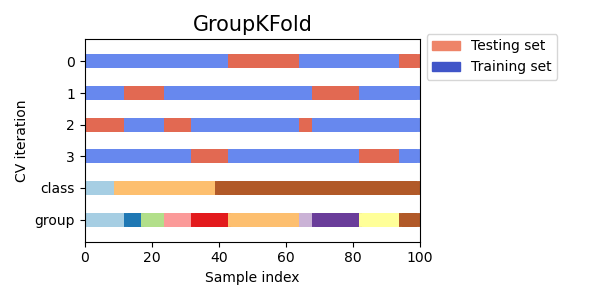
\includegraphics[width=0.75\linewidth]{Imagens/chap04/group_k_fold.png}
    \caption[Validação cruzada agrupada por regime]{Representação esquemática da validação cruzada agrupada por regime, implementada por meio do método \textit{GroupKFold}. Nesse procedimento, todas as observações pertencentes a um mesmo grupo experimental são mantidas na mesma partição, evitando que amostras correlacionadas sejam distribuídas simultaneamente entre treinamento e validação.}
    \fonte{\cite{sklearn_groupkfold_docs}.}
    \label{fig:groupkfold_validacao_metodologia}
\end{figure}

\section{Estratégia de Seleção de Modelos}
\label{sec:selecao_modelos}

A seleção de modelos neste trabalho foi estruturada de modo a considerar a organização das observações em regimes de operação e a comparação entre múltiplas famílias de modelos e combinações de hiperparâmetros. Como discutido na Fundamentação Teórica, quando muitos modelos são comparados a partir de estimativas de validação cruzada, a escolha baseada apenas no menor erro médio pode favorecer configurações que se destacam por flutuações amostrais, e não necessariamente por maior capacidade real de generalização.

Por esse motivo, a estratégia adotada não se limitou à seleção direta da configuração com menor erro médio de validação. Em vez disso, foi utilizado um procedimento hierárquico que combina três elementos principais: desempenho médio em validação cruzada, variabilidade do desempenho entre partições e parcimônia estrutural do modelo. Essa combinação busca tornar o processo de escolha mais robusto, evitando favorecer modelos excessivamente complexos quando sua vantagem de desempenho está dentro da variabilidade observada na validação.

Como definido na estratégia de validação, a métrica principal utilizada no processo de seleção foi o RMSE associado ao fluxo de permeado. Essa escolha permitiu orientar a seleção para a variável de maior interesse operacional e de maior complexidade preditiva aparente, mantendo as demais saídas no treinamento multissaída e na avaliação posterior de desempenho. Assim, a seleção foi conduzida com foco no fluxo, enquanto a análise final dos modelos considerou também a qualidade das predições das temperaturas de saída.

Dessa forma, a seleção de modelos foi conduzida em etapas sucessivas. Inicialmente, identificou-se o melhor desempenho médio em validação cruzada. Em seguida, definiu-se um conjunto de modelos candidatos dentro de uma margem de variabilidade em relação ao melhor modelo observado. Desse conjunto, selecionou-se a configuração de menor complexidade estrutural. Em caso de empate, o menor erro médio de validação foi utilizado como critério de desempate.

\subsection{Ferramentas Gráficas de Diagnóstico e Comparação dos Modelos}

Além das métricas numéricas obtidas por validação cruzada, o pipeline implementado gerou gráficos com finalidade diagnóstica e comparativa. Esses gráficos não substituem o critério formal de escolha adotado neste trabalho, mas complementam a análise ao permitir visualizar estabilidade, capacidade de generalização, comportamento do erro e qualidade preditiva para cada variável de interesse.

As principais ferramentas gráficas utilizadas são resumidas na Tabela~\ref{tab:graficos_diagnostico}.

\begin{table}[H]
\centering
\caption[Ferramentas gráficas utilizadas para diagnóstico dos modelos]{Ferramentas gráficas utilizadas para diagnóstico e comparação dos modelos ao longo do processo de seleção.}
\label{tab:graficos_diagnostico}
\begin{tabular}{p{4.3cm} p{9.5cm}}
\hline
\textbf{Gráfico} & \textbf{Finalidade} \\
\hline

Erro de validação cruzada versus complexidade
&
Avaliar o compromisso entre desempenho, variabilidade entre partições e parcimônia estrutural, evidenciando o melhor desempenho bruto, o limiar de seleção baseado em dispersão e a configuração selecionada. \\

Predito versus observado com predições \textit{out-of-fold} (OOF)
&
Avaliar a aderência entre valores previstos e valores experimentais para cada variável de saída, incluindo a reta identidade como referência visual. \\

RMSE por variável de saída
&
Comparar o desempenho dos modelos selecionados em cada parãmetro de desempenho, verificando se os ganhos se concentram no fluxo de permeado ou se também se refletem nas temperaturas de saída. \\

Curvas de aprendizagem
&
Acompanhar a evolução das perdas de treinamento e validação ao longo das épocas nos modelos neurais, auxiliando a interpretação do treinamento e do mecanismo de parada antecipada \\

Erro versus hiperparâmetro
&
Analisar a sensibilidade do modelo a um hiperparâmetro de interesse, permitindo identificar regiões de subajuste, bom compromisso entre ajuste e generalização, e possíveis sinais de sobreajuste. \\

\hline
\end{tabular}
\fonte{Elaborado pela autora.}
\end{table}

As predições \textit{out-of-fold} correspondem às previsões obtidas para cada observação quando essa observação pertence ao subconjunto de validação, isto é, quando não foi utilizada no ajuste do modelo naquela iteração. Dessa forma, os gráficos de valores preditos versus valores reais baseados em predições \textit{out-of-fold} OOF fornecem uma avaliação visual coerente com o procedimento de validação cruzada adotado.

\subsection{Critério Baseado em Um Desvio Padrão para Métricas de Erro}

Na Fundamentação Teórica, foi apresentada a regra clássica do \textit{one-standard-error}, baseada no erro padrão da média das métricas de validação. Na implementação computacional deste trabalho, entretanto, utilizou-se diretamente o atributo \texttt{std\_test\_score} fornecido pelo \texttt{GridSearchCV}, que corresponde ao desvio padrão da métrica de validação entre as partições da validação cruzada. Portanto, o critério aplicado corresponde a uma adaptação inspirada na lógica da regra \textit{one-standard-error}, mas baseada em um desvio padrão entre partições.

Seja

\begin{equation}
m^{\ast}=\arg\min_{m\in\mathcal{M}}\widehat{\mathcal{L}}^{CV}(m)
\label{eq:modelo_melhor_erro_medio}
\end{equation}

\noindent o modelo com menor erro médio estimado por validação cruzada. Para métricas de erro, define-se o limiar de seleção como

\begin{equation}
T=
\widehat{\mathcal{L}}^{CV}(m^{\ast})
+
\widehat{\sigma}^{CV}(m^{\ast}),
\label{eq:limiar_um_desvio}
\end{equation}

\noindent em que \(\widehat{\sigma}^{CV}(m^{\ast})\) representa o desvio padrão da métrica de validação entre as partições da validação cruzada para o modelo de menor erro médio.

O conjunto de modelos elegíveis segundo esse critério é dado por

\begin{equation}
\mathcal{C}=
\left\{
m\in\mathcal{M}:
\widehat{\mathcal{L}}^{CV}(m)\le T
\right\}.
\label{eq:conjunto_candidatos_um_desvio}
\end{equation}

Esse critério estabelece uma margem de tolerância em torno do melhor erro médio observado, considerando a variabilidade empírica das métricas de validação entre partições. Como utiliza o desvio padrão entre partições, e não o erro padrão da média, a margem adotada é mais ampla do que a regra clássica do \textit{one-standard-error}. Assim, o procedimento tende a favorecer a seleção de modelos mais parcimoniosos quando diferenças de desempenho estão dentro da variabilidade observada na validação cruzada.

\subsection{Critério Hierárquico de Seleção}

O critério hierárquico de seleção foi aplicado separadamente em cada busca de hiperparâmetros, isto é, dentro do conjunto de configurações candidatas pertencentes a uma mesma família de modelos. Dessa forma, nesta etapa, o objetivo não é comparar diretamente famílias distintas, mas selecionar, para cada família avaliada, a configuração de hiperparâmetros mais adequada segundo os critérios definidos.

Após a aplicação do critério baseado em um desvio padrão, obtém-se o conjunto \(\mathcal{C}\), composto pelas configurações candidatas cujo desempenho médio em validação cruzada se encontra dentro da margem de variabilidade em relação à melhor configuração observada. Em seguida, incorpora-se explicitamente um critério de parcimônia estrutural. Define-se inicialmente

\begin{equation}
C_{\min}=\min_{h\in\mathcal{C}} C(h),
\label{eq:complexidade_minima_configuracao}
\end{equation}

\noindent em que \(C(h)\) representa a medida de complexidade estrutural associada à configuração de hiperparâmetros \(h\).

Como a noção de complexidade depende da família de modelos considerada, foram adotadas medidas específicas para cada classe de modelo avaliada. Essas medidas são apresentadas na Tabela~\ref{tab:complexidade_modelos}.

Para os modelos lineares regularizados, essa medida foi definida em função do parâmetro de regularização \(\alpha\), que controla a intensidade da penalização aplicada aos coeficientes do modelo. Valores maiores de \(\alpha\) aumentam o peso da penalização e restringem mais fortemente os coeficientes, resultando em modelos efetivamente mais simples. Por outro lado, valores menores de \(\alpha\) reduzem a penalização e permitem maior liberdade de ajuste, sendo interpretados neste trabalho como configurações de maior complexidade efetiva. Por esse motivo, adotou-se a transformação \(-\log_{10}(\alpha)\) como proxy de complexidade para os modelos regularizados.

\begin{longtable}{p{4.2cm} p{9.8cm}}
\caption[Critérios de complexidade estrutural utilizados na seleção de configurações]{Critérios de complexidade estrutural utilizados na seleção de configurações de hiperparâmetros em cada família de modelos.}
\label{tab:complexidade_modelos}\\

\hline
\textbf{Família de modelos} & \textbf{Medida de complexidade adotada} \\
\hline
\endfirsthead

\hline
\textbf{Família de modelos} & \textbf{Medida de complexidade adotada} \\
\hline
\endhead

\hline
\multicolumn{2}{r}{\textit{Continua na próxima página}} \\
\endfoot

\hline
\endlastfoot

OLS &
Complexidade fixa, definida como \(C(h)=0\). \\

Ridge &
Complexidade definida por \(C(h)=-\log_{10}(\alpha)\). Menores valores de \(\alpha\) correspondem a maior complexidade efetiva. \\

Lasso e Lasso multissaída independente &
Complexidade definida por \(C(h)=-\log_{10}(\alpha)\). Na versão multissaída independente, aplica-se o mesmo critério ao estimador base. \\

ElasticNet e ElasticNet multissaída independente &
Complexidade definida por
\[
C(h)=-\log_{10}(\alpha)+0{,}01(1-l_1).
\]
O termo associado a \(l_1\) atua como ajuste secundário. \\

Árvore de decisão &
Complexidade definida principalmente pela profundidade máxima da árvore:
\[
C(h)=d-10^{-3}n_{\mathrm{leaf}},
\]
em que \(d=\texttt{max\_depth}\) e \(n_{\mathrm{leaf}}=\texttt{min\_samples\_leaf}\). Quando \(\texttt{max\_depth=None}\), atribui-se a \(d\) um valor elevado. \\

Random Forest &
Complexidade definida por
\[
C(h)=d+10^{-3}n_{\mathrm{est}}-10^{-6}n_{\mathrm{leaf}},
\]
em que \(d=\texttt{max\_depth}\), \(n_{\mathrm{est}}=\texttt{n\_estimators}\) e \(n_{\mathrm{leaf}}=\texttt{min\_samples\_leaf}\). \\

Gradient Boosting &
Complexidade definida por
\[
C(h)=d+10^{-3}n_{\mathrm{est}},
\]
em que \(d=\texttt{max\_depth}\) e \(n_{\mathrm{est}}=\texttt{n\_estimators}\). \\

MLP do \textit{scikit-learn} &
Complexidade aproximada por
\[
C(h)=\sum_{\ell=1}^{L} n_{\ell}+0{,}1L,
\]
em que \(n_{\ell}\) é o número de neurônios na camada \(\ell\) e \(L\) é o número de camadas ocultas. \\

MLP implementado em Keras e modelos neurais híbridos &
Complexidade aproximada por
\[
C(h)=\sum_{\ell=1}^{L} n_{\ell}+0{,}1L.
\]
Esse critério considera o número total de neurônios e o número de camadas ocultas. \\

\end{longtable}

Define-se então o subconjunto de configurações de menor complexidade como

\begin{equation}
\mathcal{C}_{\min}=
\left\{
h\in\mathcal{C}:
C(h)=C_{\min}
\right\}.
\label{eq:conjunto_complexidade_minima_configuracao}
\end{equation}

Caso múltiplas configurações apresentem a mesma complexidade mínima, utiliza-se o menor erro médio de validação entre elas como critério de desempate, selecionando-se

\begin{equation}
\widehat{h}=
\arg\min_{h\in\mathcal{C}_{\min}}
\widehat{\mathcal{L}}^{CV}(h).
\label{eq:configuracao_final_empate}
\end{equation}

A configuração \(\widehat{h}\) é então adotada como a configuração selecionada para a família de modelos considerada. Após a aplicação desse procedimento em cada família, os modelos resultantes, já com suas respectivas configurações selecionadas, são comparados entre si com base nas métricas de desempenho obtidas por validação cruzada. Dessa forma, o processo distingue duas etapas: primeiro, a seleção da configuração de hiperparâmetros dentro de cada família; depois, a comparação entre os modelos finais representantes de cada família.

\subsection{Comparação entre Famílias por Contagem de Parâmetros}

Enquanto a seleção dentro de cada família utilizou medidas de complexidade específicas para cada classe de modelo, a comparação entre famílias distintas empregou uma métrica universal: o número total de parâmetros treináveis de cada arquitetura. Essa abordagem permitiu posicionar modelos de naturezas fundamentalmente diferentes -- regressão linear, redes neurais e arquiteturas híbridas -- em uma mesma escala de complexidade.

O número de parâmetros de cada modelo foi calculado analiticamente a partir de sua arquitetura. Para a regressão linear (\texttt{OLS}), com cinco variáveis de entrada e três saídas, o total é de 18 parâmetros (15 coeficientes e 3 interceptos). Para as redes neurais e arquiteturas híbridas, a contagem depende do número de neurônios em cada camada, sendo a quantidade de parâmetros de uma camada densa dada por \(n_{\mathrm{in}} \times n_{\mathrm{out}} + n_{\mathrm{out}}\).

Como as buscas de hiperparâmetros foram conduzidas de forma independente para cada alvo, as arquiteturas selecionadas diferem entre si. Para os alvos \(T_{\mathrm{alim,out}}\) e \(T_{\mathrm{ref,out}}\), a configuração vencedora utiliza duas camadas ocultas com 128 e 64 neurônios e ativação \texttt{tanh}, totalizando 9219 parâmetros. Para o alvo \(Flux\), a configuração vencedora utiliza três camadas ocultas com 128, 64 e 32 neurônios e ativação \texttt{relu}, totalizando 11203 parâmetros.

Nas arquiteturas híbridas que utilizam todas as oito variáveis de entrada (cinco experimentais mais três predições físicas), como HPD e HRNN, a primeira camada recebe três entradas adicionais, acrescentando 384 parâmetros ao total. Dessa forma, para as baselines de \(T_{\mathrm{alim,out}}\) e \(T_{\mathrm{ref,out}}\), as arquiteturas HPD e HRNN totalizam 9603 parâmetros; para a baseline de \(Flux\), totalizam 11587 parâmetros. A arquitetura residual (ZohanResidual), embora receba as oito variáveis como entrada, aplica a rede neural apenas ao subconjunto de cinco variáveis experimentais e combina a saída por soma à predição física -- o que resulta na mesma contagem de parâmetros da baseline neural correspondente a cada alvo (9219 ou 11203, respectivamente).

Após o cálculo do número de parâmetros, aplicou-se novamente o critério baseado em um desvio padrão (1-SE), agora sobre o conjunto de todos os modelos candidatos de diferentes famílias. Entre os modelos dentro da margem de um desvio padrão do melhor desempenho, priorizou-se a arquitetura de menor número de parâmetros, retomando a lógica de parcimônia em uma escala comum de complexidade.

\begin{figure}[H]
    \centering
    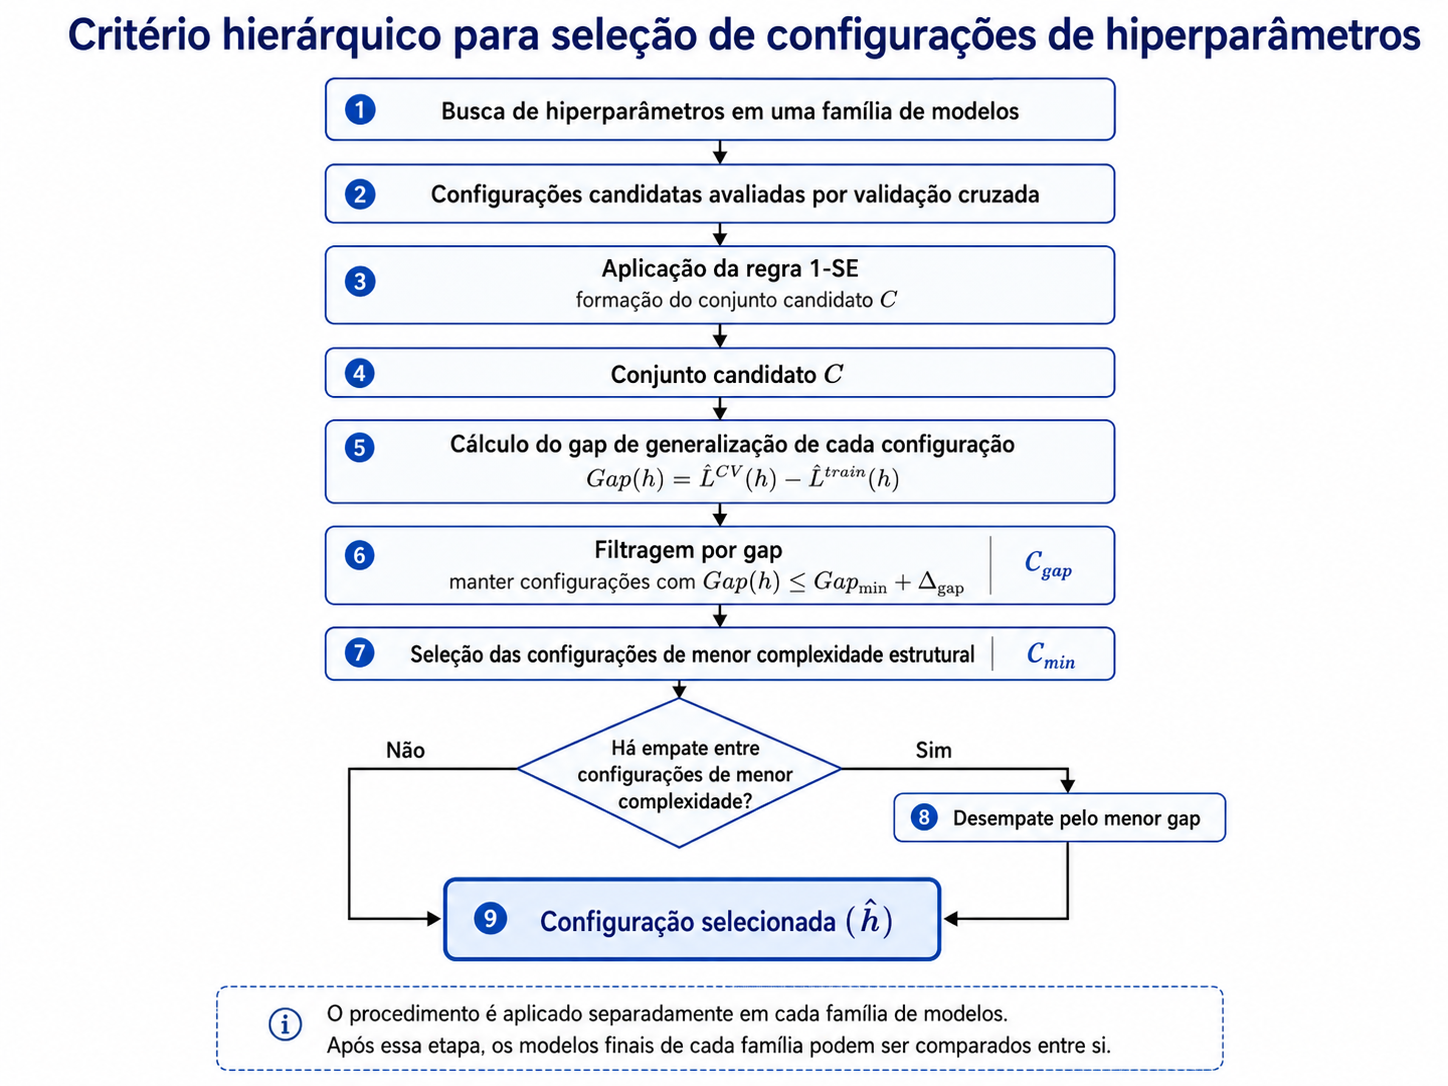
\includegraphics[width=1\linewidth]{Imagens/chap04/esquema_comp.png}
    \caption[Critério hierárquico de seleção de configurações]{Representação esquemática do critério hierárquico utilizado para selecionar a configuração de hiperparâmetros dentro de cada família de modelos. A partir do conjunto de configurações candidatas obtido após a aplicação do critério baseado em um desvio padrão, selecionam-se as configurações de menor complexidade estrutural e, em caso de empate, utiliza-se o menor erro médio de validação como critério final de desempate. Fonte: Elaborado pela Autora}

    \label{fig:criterio_hierarquico_selecao}
\end{figure}
\subsection{Implementação Computacional}

O procedimento foi implementado por meio do \texttt{GridSearchCV}, utilizando:

\begin{itemize}
    \item validação cruzada baseada em \textit{GroupKFold};
    \item encapsulamento das etapas de pré-processamento e modelagem em \textit{Pipeline}, garantindo que transformações dependentes dos dados, como a padronização, fossem ajustadas apenas no subconjunto de treinamento de cada partição;
    \item cálculo simultâneo dos erros de treinamento e validação, por meio de \texttt{return\_train\_score=True};
    \item função personalizada de \texttt{refit}, responsável por implementar o critério baseado em um desvio padrão, seguido da minimização da complexidade estrutural e do desempate final pelo menor erro de validação.
\end{itemize}

A utilização direta das estatísticas disponíveis em \texttt{cv\_results\_}, como \texttt{mean\_test\_score}, \texttt{std\_test\_score}, permitiu integrar avaliação de desempenho, variabilidade entre partições e parcimônia estrutural em um único procedimento de seleção calibrada.
\section{Estrutura Computacional da Comparação entre Modelos}

A implementação computacional do procedimento de modelagem foi estruturada como um pipeline unificado de comparação entre famílias de modelos. Esse pipeline integra as etapas de pré-processamento, busca de hiperparâmetros, validação cruzada e seleção final de modelos em um fluxo reprodutível.

O objetivo dessa organização é garantir que todas as famílias avaliadas sejam submetidas ao mesmo protocolo de avaliação, permitindo comparações consistentes de desempenho e evitando diferenças artificiais decorrentes de procedimentos distintos de treinamento ou validação.

\subsection{Organização geral do pipeline}

O processo de modelagem foi estruturado em três etapas principais, mantendo-se, em todas elas, o mesmo protocolo geral de avaliação: validação cruzada agrupada por \textit{Regime}, cálculo das métricas de desempenho em treino e validação e seleção de configurações com base no critério hierárquico descrito anteriormente. As diferenças entre as etapas dizem respeito principalmente às famílias de modelos avaliadas e à extensão da busca de hiperparâmetros realizada.

Na primeira etapa, foram avaliados modelos clássicos de regressão supervisionada, incluindo modelos lineares, modelos lineares regularizados e modelos baseados em árvores. Para essas famílias, a busca de hiperparâmetros foi conduzida por meio de \texttt{GridSearchCV}, utilizando validação cruzada baseada em \textit{GroupKFold}. Nos modelos sensíveis à escala das variáveis, as etapas de pré-processamento foram encapsuladas em \textit{Pipeline}, garantindo que a padronização das variáveis de entrada fosse ajustada apenas sobre os dados de treinamento de cada partição.

Na segunda etapa, foram avaliadas redes neurais do tipo \textit{Multi-Layer Perceptron}. Também nessa etapa, a seleção de configurações foi realizada por meio de \texttt{GridSearchCV} associado ao \textit{GroupKFold}, permitindo comparar diferentes arquiteturas sob o mesmo procedimento de validação adotado para os demais modelos. Devido ao maior custo computacional associado ao treinamento dessas arquiteturas, a busca foi limitada a grades previamente definidas de hiperparâmetros, contemplando combinações de tamanho da rede, regularização e parâmetros de treinamento.

Na terceira etapa, foram investigadas estratégias híbridas que integram estimativas provenientes do modelo físico reduzido ao processo de aprendizado das redes neurais, conforme descrito na Seção~\ref{sec:modelos-hibridos}. Nessa fase, a busca de hiperparâmetros foi restringida a arquiteturas previamente identificadas como competitivas, reduzindo o espaço de busca e o custo computacional total. Assim como nas etapas anteriores, a avaliação foi conduzida por validação cruzada agrupada, preservando a separação por \textit{Regime}.

Essa estrutura sequencial permite comparar famílias de modelos sob um procedimento de avaliação comum, ao mesmo tempo em que controla o custo computacional da análise. A organização em etapas também possibilita verificar, de forma progressiva, se o aumento de complexidade estrutural — de modelos clássicos para redes neurais e, posteriormente, para abordagens híbridas — resulta em ganhos efetivos de desempenho preditivo.
\subsection{Estratégias de redução de custo computacional}

O treinamento de modelos de aprendizado de máquina, particularmente redes neurais, pode envolver elevado custo computacional quando múltiplas combinações de hiperparâmetros são avaliadas sob validação cruzada. Para tornar o processo viável, foram adotadas estratégias específicas de otimização do treinamento.

Para os modelos neurais implementados em \texttt{Keras}, utilizou-se o mecanismo de parada antecipada (do inglês, \textit{early stopping}, no qual o treinamento é interrompido automaticamente quando a perda de validação deixa de apresentar melhora significativa após um número predefinido de épocas. Essa estratégia evita treinamento desnecessário após a convergência do modelo.

Adicionalmente, empregou-se o mecanismo de redução adaptativa da taxa de aprendizado (\textit{learning rate scheduling}), no qual a taxa de aprendizado é automaticamente reduzida quando o desempenho de validação permanece estagnado por um determinado número de épocas. Essa estratégia permite refinar o processo de otimização próximo ao mínimo da função de perda.

Também foi utilizado um mecanismo de interrupção automática em caso de instabilidade numérica (\texttt{TerminateOnNaN}), garantindo robustez durante o treinamento.

Essas estratégias combinadas permitem reduzir significativamente o tempo total de treinamento sem comprometer a qualidade das soluções encontradas.

\subsection{Geração automática de análises gráficas}

Além das métricas numéricas obtidas na validação cruzada, o pipeline foi estruturado para gerar automaticamente um conjunto de análises gráficas utilizadas na interpretação dos resultados.

Entre os artefatos gráficos produzidos estão:

\begin{itemize}
\item gráficos de desempenho em função da complexidade estrutural dos modelos;
\item gráficos de valores previstos versus valores experimentais obtidos a partir de predições \textit{out-of-fold};
\item curvas de treinamento e validação para as arquiteturas neurais;
\item análises de sensibilidade local do erro em relação aos hiperparâmetros principais;
\item gráficos comparativos de desempenho entre modelos para cada variável-alvo.
\end{itemize}

Essas representações visuais auxiliam na interpretação do comportamento dos modelos, permitindo identificar tendências de sobreajuste, regimes de complexidade adequada e diferenças de desempenho entre famílias de modelos.

\subsection{Avaliação Final por Predições \textit{Out-of-Fold} (OOF)}
\label{sec:avaliacao_oof}

Conforme discutido na Seção~\ref{sec:selecao_modelos}, o critério hierárquico de seleção utiliza o erro médio de validação cruzada (CV RMSE) para comparar e escolher a configuração de hiperparâmetros de cada família. No entanto, essa estimativa pode apresentar viés otimista, uma vez que o mesmo conjunto de validação cruzada é empregado tanto para selecionar a configuração quanto para estimar seu desempenho, favorecendo configurações que se destacam por flutuações amostrais (\cite{Cawley2010Overfitting}).

Para obter uma estimativa menos tendenciosa do desempenho preditivo, adotou-se um procedimento de predições \textit{out-of-fold} (OOF). Após a seleção da configuração ótima, um novo modelo é instanciado com os hiperparâmetros escolhidos e retreinado independentemente em cada partição da validação cruzada, partindo de uma nova inicialização aleatória. As predições sobre as amostras mantidas fora do treinamento em cada partição são então concatenadas, formando um conjunto completo de predições. Diferentemente da função \texttt{cross\_val\_predict} do \textit{scikit-learn}, que retorna predições obtidas durante o próprio processo de validação cruzada e não é recomendada como medida de erro de generalização (\cite{sklearn_cv_docs}), o procedimento aqui adotado realiza um re-treinamento independente do modelo selecionado em cada partição, produzindo uma estimativa de desempenho posterior ao processo de seleção.

As métricas finais de desempenho reportadas neste trabalho (RMSE OOF e R$^2$ OOF) são calculadas sobre essas predições concatenadas, garantindo que cada amostra seja prevista por um modelo que não a utilizou durante o treinamento.

\section{Famílias de Modelos Avaliadas}

A seleção das famílias de modelos avaliadas neste trabalho foi conduzida com o objetivo de comparar abordagens de regressão supervisionada com diferentes níveis de flexibilidade estrutural, interpretabilidade e capacidade de representação. Como o conjunto de dados envolve variáveis operacionais contínuas e múltiplas variáveis de saída, buscou-se avaliar desde modelos mais simples e parcimoniosos até métodos com maior capacidade de capturar relações não lineares entre as entradas e as respostas do sistema.


Dessa forma, a comparação entre famílias de modelos permite investigar empiricamente a adequabilidade dos modelos lineares como referência de baixa complexidade, verificando se formulações mais simples são capazes de representar satisfatoriamente a relação entre as variáveis operacionais e as respostas do sistema. Além disso, possibilita avaliar o ganho de desempenho associado à inclusão de modelos não lineares, por meio da comparação entre modelos lineares, modelos baseados em árvores e redes neurais sob o mesmo protocolo de validação cruzada. Essa análise também permite examinar o efeito do aumento de flexibilidade estrutural sobre a capacidade de generalização, considerando conjuntamente o erro de validação e a complexidade estrutural. Por fim, a comparação entre famílias fornece subsídios para avaliar o compromisso entre desempenho preditivo, estabilidade entre partições e parcimônia, levando em conta as métricas médias de validação cruzada, a variabilidade entre partições e a complexidade da configuração selecionada em cada família de modelos.

\subsection{Modelos Lineares}

Os modelos lineares (OLS, Ridge, Lasso, Elastic Net e variantes multi-task) representam a classe de menor flexibilidade estrutural considerada neste trabalho.

Sua inclusão é justificada por três razões principais:

\begin{enumerate}
    \item Servem como modelo de referência (\emph{baseline}), permitindo quantificar o ganho obtido com o aumento de flexibilidade estrutural;
    \item São consistentes com a hipótese de comportamento aproximadamente afim das temperaturas de saída;
    \item Permitem controle explícito da complexidade via regularização, favorecendo estabilidade em cenários com número limitado de observações.
\end{enumerate}

As variantes regularizadas possibilitam investigar o impacto da penalização sobre o compromisso viés--variância, sendo particularmente relevantes quando há potencial multicolinearidade entre variáveis operacionais.

\subsection{Modelos Baseados em Árvores}

Os modelos baseados em árvores, incluindo Árvore de Decisão, Random Forest e Gradient Boosting, introduzem flexibilidade não linear por meio de particionamentos sucessivos do espaço de atributos. A partir desses particionamentos, tais modelos conseguem representar relações não lineares e interações entre variáveis de entrada sem que essas relações precisem ser especificadas previamente na formulação do modelo. Dessa forma, a estrutura do modelo é construída de maneira orientada pelos padrões observados nos dados, permitindo que diferentes regiões do espaço de entrada sejam associadas a comportamentos distintos das variáveis de saída.

A inclusão dessa família permite avaliar se métodos não lineares baseados em particionamento do espaço de entrada oferecem ganhos consistentes de desempenho em relação aos modelos lineares, mantendo um nível intermediário de complexidade estrutural. A Árvore de Decisão fornece uma representação mais simples e interpretável, enquanto os métodos de ensemble, como Random Forest e Gradient Boosting, ampliam a capacidade preditiva ao combinar múltiplas árvores. No caso do Random Forest, essa combinação contribui para reduzir a variância associada a árvores individuais; já no Gradient Boosting, as árvores são ajustadas de forma sequencial, buscando corrigir os erros residuais dos modelos anteriores.
\subsection{Redes Neurais}

As redes neurais do tipo Multi-Layer Perceptron (MLP) representam a classe de maior flexibilidade estrutural considerada.

Como aproximadores universais de funções contínuas, são capazes de modelar relações altamente não lineares e interações complexas entre variáveis. Sua inclusão tem dois objetivos principais:

\begin{enumerate}
    \item Avaliar se o aumento substancial de capacidade representacional produz ganhos significativos de desempenho no domínio experimental considerado.
    \item Investigar o limite superior de flexibilidade necessário para capturar o comportamento conjunto das variáveis-alvo.
\end{enumerate}

Ao incluir redes neurais na comparação, torna-se possível verificar se a estrutura física subjacente pode ser adequadamente representada por modelos de complexidade moderada ou se demanda representações mais expressivas.

\subsection{Comparação entre Níveis de Flexibilidade Estrutural}

A seleção dessas três famílias estabelece um espectro crescente de flexibilidade estrutural:

\begin{center}
Modelos Lineares $\rightarrow$ Árvores $\rightarrow$ Redes Neurais
\end{center}

Essa organização permite confrontar as hipóteses físicas iniciais com evidências empíricas obtidas sob validação cruzada estruturada por grupos experimentais, mantendo coerência entre fundamentação física e estratégia estatística de modelagem.
\section{Tuning de Hiperparâmetros}
\label{sec:tuning}

O procedimento de \textit{tuning} tem como objetivo explorar o espaço de hiperparâmetros $\Theta_{\mathcal{F}}$ de cada família de modelos, gerando o conjunto de configurações candidatas que posteriormente serão avaliadas segundo a estratégia hierárquica de seleção descrita na Seção~4.4. Assim, o \textit{tuning} não constitui, por si só, o critério final de escolha, mas sim a etapa de geração sistemática de alternativas estruturais dentro de cada família considerada.

\subsubsection{Procedimento de busca e validação}

A busca de hiperparâmetros foi conduzida conforme o protocolo de validação descrito na Seção~\ref{sec:validacao_cruzada}, utilizando validação cruzada agrupada por \textit{Regime}. Dessa forma, todas as configurações avaliadas foram comparadas sob a mesma estrutura de particionamento, preservando a separação entre regimes experimentais durante o treinamento e a validação.

Para todas as famílias avaliadas, as etapas de pré-processamento e modelagem foram organizadas em uma estrutura única de execução, de modo que as transformações dependentes dos dados fossem ajustadas apenas no subconjunto de treinamento de cada partição. Em particular, a padronização das variáveis de entrada foi realizada por meio do procedimento de média zero e variância unitária, conforme descrito anteriormente. Além disso, em algumas famílias de modelos foi utilizado um procedimento análogo para escalonamento das variáveis de saída, permitindo que o treinamento fosse realizado no espaço padronizado das variáveis-alvo e que as predições fossem posteriormente convertidas para a escala física original.

Embora os modelos tenham sido treinados para prever simultaneamente as três variáveis de saída consideradas, o processo de seleção de hiperparâmetros foi orientado prioritariamente pelo desempenho associado ao fluxo de permeado. Essa definição é coerente com a estratégia metodológica adotada, na qual o fluxo foi tratado como a variável crítica de seleção por representar diretamente a produtividade do sistema e por apresentar maior complexidade preditiva aparente nas análises preliminares.

Para implementar esse critério, utilizou-se uma função de pontuação personalizada baseada no RMSE da variável de fluxo. Como o procedimento computacional de busca de hiperparâmetros realiza a maximização da função de pontuação, essa métrica foi implementada como o negativo do RMSE, de modo que maximizar a pontuação equivale, na prática, a minimizar o erro associado ao fluxo de permeado. As demais variáveis de saída foram mantidas no treinamento multissaída e avaliadas posteriormente, permitindo verificar se a priorização do fluxo preservava a capacidade do modelo de predizer adequadamente as temperaturas de saída do sistema.

Para isso, utilizou-se uma função de pontuação personalizada baseada no RMSE da variável de fluxo. Como o procedimento computacional de busca de hiperparâmetros realiza a maximização da função de pontuação, essa métrica foi implementada como o negativo do RMSE, de modo que maximizar a pontuação equivale, na prática, a minimizar o erro associado ao fluxo de permeado. Ainda assim, as demais variáveis de saída foram mantidas no treinamento e avaliadas posteriormente, permitindo verificar se a priorização do fluxo não comprometia de forma significativa a predição das temperaturas de saída.


\subsection{Espaços de busca por família}
\label{subsec:espacos_busca}

Os espaços de busca foram definidos de modo a abranger diferentes níveis de flexibilidade estrutural dentro de cada família de modelos, mantendo coerência com a definição operacional de complexidade adotada neste trabalho. Nas regressões regularizadas, o parâmetro \(\alpha\) controla a intensidade da penalização aplicada aos coeficientes: valores maiores de \(\alpha\) impõem maior regularização, enquanto valores menores reduzem esse efeito. No caso do Elastic Net, o parâmetro \(l_1\text{-ratio}\) controla a combinação entre as penalizações \(L_1\) e \(L_2\).

\begin{longtable}{p{3.8cm} p{9.8cm}}
\caption[Espaços de busca de hiperparâmetros por família de modelos]{Espaços de busca de hiperparâmetros avaliados para cada família de modelos.}
\label{tab:espacos_busca_modelos}\\

\hline
\textbf{Família/modelo} & \textbf{Espaço de busca avaliado} \\
\hline
\endfirsthead

\hline
\textbf{Família/modelo} & \textbf{Espaço de busca avaliado} \\
\hline
\endhead

\hline
\multicolumn{2}{r}{\textit{Continua na próxima página}} \\
\endfoot

\hline
\endlastfoot

OLS
&
Sem hiperparâmetros. Utilizado como referência linear sem regularização. \\

Ridge
&
\(\alpha \in \{10^{-3},10^{-2},10^{-1},1,10,100\}\). \\

Lasso MultiTask
&
\(\alpha \in \{10^{-4},10^{-3},10^{-2},10^{-1},1\}\). \\

ElasticNet MultiTask
&
\(\alpha \in \{10^{-4},10^{-3},10^{-2},10^{-1},1\}\);
\(l_1\text{-ratio} \in \{0{,}1,0{,}3,0{,}5,0{,}7,0{,}9\}\). \\

Lasso independente multissaída
&
\(\alpha \in \{10^{-4},10^{-3},10^{-2},10^{-1},1\}\). Implementado por meio de estimadores independentes para cada saída. \\

ElasticNet independente multissaída
&
\(\alpha \in \{10^{-4},10^{-3},10^{-2},10^{-1},1\}\);
\(l_1\text{-ratio} \in \{0{,}1,0{,}3,0{,}5,0{,}7,0{,}9\}\). Implementado por meio de estimadores independentes para cada saída. \\

Árvore de decisão
&
\(\texttt{max\_depth} \in \{2,3,4,5,6,\texttt{None}\}\);
\(\texttt{min\_samples\_leaf} \in \{1,2,5,8,10\}\);
\(\texttt{min\_samples\_split} \in \{2,5,10,15\}\);
\(\texttt{ccp\_alpha} \in \{0,10^{-4},10^{-3},10^{-2}\}\). \\

Random Forest
&
\(\texttt{n\_estimators} \in \{200,400,600\}\);
\(\texttt{max\_depth} \in \{2,3,4,5,\texttt{None}\}\);
\(\texttt{min\_samples\_leaf} \in \{1,2,5,8,10\}\);
\(\texttt{min\_samples\_split} \in \{2,5,10\}\);
\(\texttt{max\_features} \in \{0{,}5,0{,}8,1{,}0\}\). \\

Gradient Boosting
&
\(\texttt{n\_estimators} \in \{50,100,200,400\}\);
\(\texttt{learning\_rate} \in \{0{,}01,0{,}03,0{,}05,0{,}1\}\);
\(\texttt{max\_depth} \in \{1,2,3\}\);
\(\texttt{min\_samples\_leaf} \in \{1,2,5,10\}\);
\(\texttt{subsample} \in \{0{,}6,0{,}8,1{,}0\}\).
Utilizou-se modelagem independente para viabilizar a predição multissaída. \\

MLP no \textit{scikit-learn}
&
\(\texttt{hidden\_layer\_sizes} \in \{(32,), (64,), (64,32), (128,64)\}\);
\(\alpha \in \{0,10^{-6},10^{-5},10^{-4}\}\);
\(\texttt{learning\_rate\_init} \in \{3\times10^{-3},10^{-3},3\times10^{-4},10^{-4}\}\). \\

KerasMLP baseline
&
\(\texttt{hidden\_layer\_sizes} \in \{(32,), (64,), (128,), (256,), (64,32), (128,64), (256,128), (128,64,32), (256,128,64)\}\);
\(\texttt{learning\_rate} \in \{10^{-3},3\times10^{-4}\}\);
\(\texttt{l2} \in \{0,10^{-6},10^{-5}\}\).
Foram mantidos fixos: ativação ReLU, otimizador Adam, função de perda Huber, \(\delta=1{,}0\), lote de 64 amostras, 200 épocas e fração de validação interna de 0,2. \\

KerasMLP FrozenBaseline
&
Utiliza diretamente a configuração baseline selecionada, sem variação adicional relevante de hiperparâmetros. Atua como referência neural não híbrida. \\

KerasMLP Luc Restricted
&
Mantém a estrutura da baseline e varia os hiperparâmetros associados ao termo físico na função de perda:
\(\texttt{physics\_norm} \in \{\texttt{mse},\texttt{mae}\}\);
\(\omega \in \{0{,}0,0{,}1,0{,}3,0{,}5,0{,}7\}\). \\

KerasMLP ZohanHPD Restricted
&
Utiliza como entrada o vetor experimental concatenado às predições físicas. A busca é restrita a uma vizinhança do parâmetro \(l_2\):
\(\texttt{l2} \in \{\texttt{l2}_{base},0,10^{-6},10^{-5},10^{-4}\}\). \\

KerasMLP ZohanResidual Restricted
&
Adota arquitetura residual baseada na soma entre a predição física e uma correção aprendida. A busca é restrita a uma vizinhança do parâmetro \(l_2\):
\(\texttt{l2} \in \{\texttt{l2}_{base},0,10^{-6},10^{-5},10^{-4}\}\). \\

KerasMLP ZohanHRNN Restricted
&
Combina entrada expandida com correção residual, mantendo a configuração baseline como referência. A busca é restrita ao parâmetro \(l_2\):
\(\texttt{l2} \in \{\texttt{l2}_{base},0,10^{-6},10^{-5},10^{-4}\}\). \\

\end{longtable}

A organização em tabela permite explicitar, de forma compacta, quais hiperparâmetros foram efetivamente explorados em cada família. Nos modelos lineares regularizados, a busca concentra-se principalmente na intensidade da penalização. Nos modelos baseados em árvores, os hiperparâmetros controlam a profundidade, o número de estimadores e o tamanho mínimo das partições. Nas redes neurais, a busca envolve principalmente arquitetura, taxa de aprendizado e regularização. Já nas famílias híbridas, a busca foi restringida a hiperparâmetros específicos, mantendo como referência a configuração neural baseline previamente selecionada.

\section{Uso do Modelo Físico na Estratégia de Modelagem}

O modelo físico reduzido do módulo de dessalinização, previamente descrito na Fundamentação Teórica, não constitui o objeto de desenvolvimento deste trabalho, mas é empregado como elemento auxiliar na estratégia de modelagem supervisionada proposta.

\subsection{Papel Metodológico}

Neste estudo, o modelo físico desempenha duas funções principais: (i) atuar como referência comparativa para avaliação do desempenho dos modelos orientados a dados e (ii) integrar estratégias híbridas de aprendizado, nas quais informações físicas são incorporadas ao processo de treinamento das redes neurais.

Dessa forma, o modelo físico fornece uma base interpretativa fundamentada em princípios de conservação e termodinâmicos, permitindo analisar em que medida abordagens puramente orientadas a dados são capazes de reproduzir, corrigir ou superar seu desempenho preditivo.

\subsection{Integração Híbrida e Comparação com Modelos Baseados em Dados}

Nas estratégias híbridas avaliadas, o modelo físico é utilizado não apenas como referência comparativa, mas também como fonte de conhecimento adicional incorporado ao processo de aprendizado dos modelos baseados em dados.

A integração entre conhecimento físico e aprendizado de máquina pode ser realizada de diferentes formas, dependendo da maneira como a informação proveniente do modelo físico é utilizada durante o treinamento. Neste trabalho, foram investigadas diferentes estratégias de integração físico--dados, tomando o modelo físico reduzido como fonte de informação estruturada para auxiliar o aprendizado supervisionado.

Além das arquiteturas híbridas propriamente ditas, a comparação incluiu também uma rede neural baseline com hiperparâmetros congelados, utilizada como referência para avaliar em que medida a incorporação explícita de informação física produz ganhos efetivos de desempenho.

\subsection{Estratégias de Integração Físico--Dados}

Com o objetivo de avaliar diferentes formas de incorporar conhecimento físico ao processo de aprendizado, foram implementadas quatro estratégias de modelagem híbrida físico--dados. Essas estratégias diferem quanto ao papel atribuído à predição do modelo físico reduzido: ela pode ser utilizada como variável adicional de entrada, como aproximação inicial a ser corrigida pela rede neural, como componente simultâneo de entrada e correção residual, ou ainda como termo auxiliar na função de perda.

Em particular, as três primeiras estratégias seguem formas de integração discutidas na literatura de \textit{physics-informed machine learning}, nas quais o modelo físico pode atuar como fonte adicional de informação, como referência inicial para uma correção residual ou como parte da arquitetura híbrida da rede \cite{zhou2025physics}. A Figura~\ref{fig:hrnn_model} apresenta essas três arquiteturas de forma esquemática, servindo como referência visual para as subseções seguintes. A estrutura (A) corresponde ao modelo \textit{Hybrid Physics Data} (HPD), em que a predição física é concatenada às variáveis experimentais de entrada. A estrutura (B) corresponde ao modelo residual, no qual a rede neural aprende uma correção a ser somada à predição física. Por fim, a estrutura (C) corresponde ao modelo \textit{Hybrid Residual Neural Network} (HRNN), que combina simultaneamente a entrada física auxiliar e a correção residual.

\begin{figure}[H]
\centering
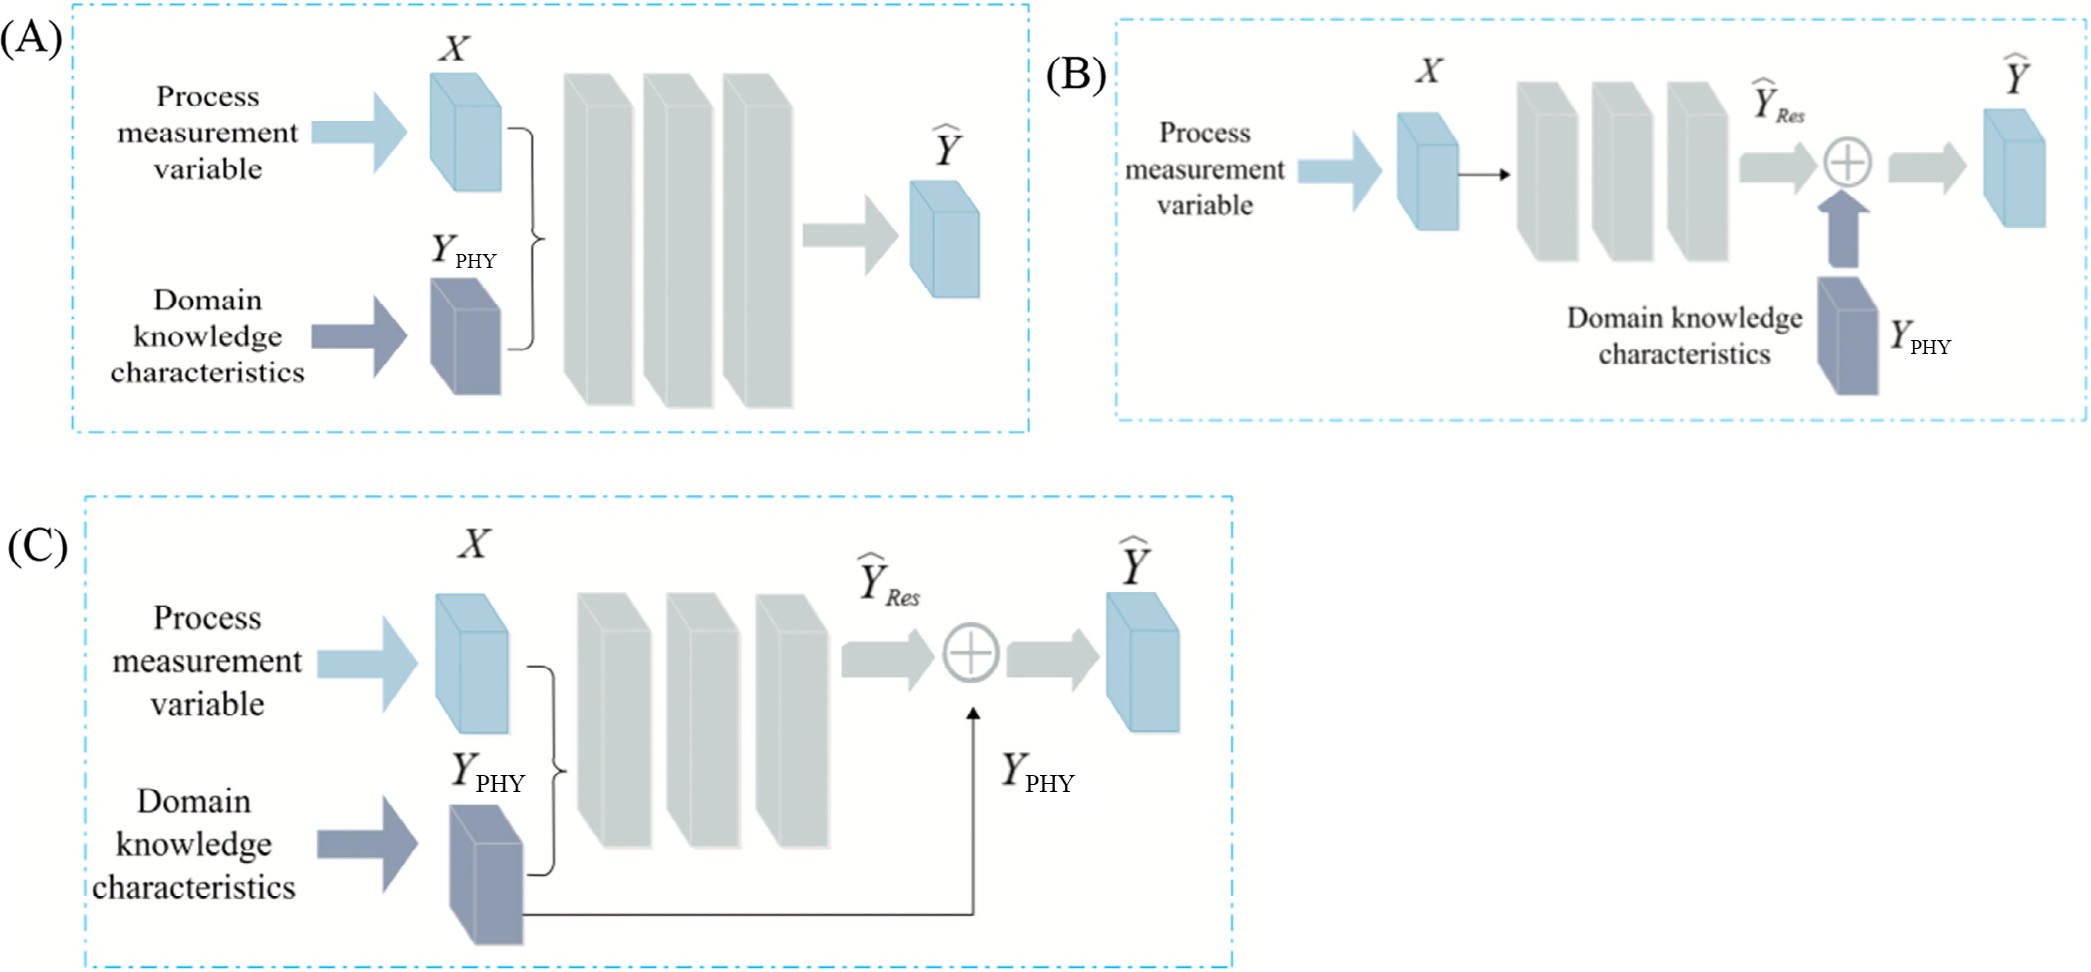
\includegraphics[width=1.0\textwidth]{Imagens/chap04/hybrids.png}
\caption[Estratégias híbridas físico--dados implementadas no trabalho]{Representação esquemática das estratégias híbridas físico--dados implementadas neste trabalho. As estruturas (A), (B) e (C) correspondem, respectivamente, ao modelo \textit{Hybrid Physics Data} (HPD), ao modelo residual e ao modelo \textit{Hybrid Residual Neural Network} (HRNN). Em (A), a predição do modelo físico é utilizada como entrada adicional da rede neural; em (B), a rede aprende um termo residual somado à predição física; e, em (C), essas duas estratégias são combinadas em uma única arquitetura. Fonte: adaptado de \cite{zhou2025physics}.}
\label{fig:hrnn_model}
\end{figure}

\subsubsection{Modelo Híbrido com Predições Físicas como Variáveis de Entrada (HPD)}

A primeira estratégia consiste em utilizar diretamente as predições do modelo físico reduzido como variáveis adicionais de entrada da rede neural. Essa abordagem corresponde ao modelo híbrido \textit{Hybrid Physics Data} (HPD), representado esquematicamente na Figura~\ref{fig:hrnn_model}(A) \cite{zhou2025physics}.

Se \(\mathbf{X}\) representa o vetor de variáveis experimentais de entrada e \(Y_{\text{PHY}}\) representa a predição fornecida pelo modelo físico, o vetor de entrada expandido pode ser definido como

\begin{equation}
\mathbf{X}' = [\mathbf{X}, Y_{\text{PHY}}].
\end{equation}

Dessa forma, a rede neural recebe simultaneamente informações provenientes das condições operacionais medidas e das estimativas produzidas pelo modelo físico. A função da rede, nesse caso, é aprender a relação entre esse conjunto expandido de entradas e as respostas experimentais, podendo explorar complementaridades entre as variáveis medidas e a aproximação física disponível.

\subsubsection{Modelagem Residual Baseada no Modelo Físico}

A segunda estratégia consiste em utilizar o modelo físico como uma aproximação inicial do sistema e treinar a rede neural para aprender uma correção residual. Essa formulação corresponde à estrutura representada na Figura~\ref{fig:hrnn_model}(B), associada à modelagem híbrida residual \cite{zhou2025physics}.

Seja \(Y_{\text{PHY}}\) a predição fornecida pelo modelo físico e \(Y\) o valor experimental observado. Conceitualmente, o resíduo associado ao modelo físico pode ser definido como

\begin{equation}
Y_{\text{res}} = Y - Y_{\text{PHY}}.
\end{equation}

Na implementação adotada neste trabalho, a rede neural não foi treinada a partir de um conjunto-alvo residual explicitamente separado. Em vez disso, a arquitetura foi construída de modo que sua saída representasse diretamente uma correção aprendida sobre a predição física. Assim, a predição final do modelo assume a forma

\begin{equation}
\hat{Y} = Y_{\text{PHY}} + \hat{Y}_{\text{res}},
\end{equation}

\noindent em que \(\hat{Y}_{\text{res}}\) corresponde ao termo corretivo produzido pela rede neural. Nessa abordagem, o modelo físico fornece uma estimativa inicial, enquanto a rede neural aprende a compensar desvios sistemáticos em relação aos dados experimentais.

\subsubsection{Hybrid Residual Neural Network (HRNN)}

A terceira estratégia combina as duas abordagens anteriores em uma única arquitetura, denominada \textit{Hybrid Residual Neural Network} (HRNN). Essa formulação corresponde à estrutura representada na Figura~\ref{fig:hrnn_model}(C) \cite{zhou2025physics}.

Nesse caso, a rede neural utiliza simultaneamente as variáveis experimentais e a predição do modelo físico como entradas, ao mesmo tempo em que produz uma correção residual somada à estimativa física. Portanto, diferentemente do HPD, em que a predição física atua apenas como variável adicional de entrada, e do modelo residual, em que a rede aprende apenas a correção sobre a estimativa física, o HRNN integra os dois mecanismos na mesma arquitetura.

Matematicamente, a predição final pode ser representada por

\begin{equation}
\hat{Y} = f_{NN}(X, Y_{\text{PHY}}) + Y_{\text{PHY}},
\end{equation}

\noindent em que \(f_{NN}(X, Y_{\text{PHY}})\) representa o termo corretivo aprendido pela rede a partir das variáveis experimentais e das predições do modelo físico.

Nesse contexto, o modelo físico fornece uma aproximação inicial do comportamento do sistema, enquanto a rede neural aprende a corrigir vieses sistemáticos e desvios estruturais em relação aos dados experimentais. Dessa forma, o HRNN busca combinar a informação fenomenológica fornecida pelo modelo reduzido com a flexibilidade de representação da rede neural.

\subsubsection{Regularização da Função de Perda com Predições do Modelo Físico}

A quarta estratégia de integração físico--dados consiste em incorporar diretamente as predições do modelo físico à função de perda utilizada no treinamento da rede neural. Diferentemente das três arquiteturas apresentadas na Figura~\ref{fig:hrnn_model}, essa abordagem não altera necessariamente o vetor de entrada ou a forma da predição final, mas modifica o critério de treinamento da rede ao incluir uma penalização associada à discrepância em relação ao modelo físico. Essa estratégia foi explorada por \cite{seixo2024internship} no contexto da modelagem de sistemas de destilação por membranas.

Nessa formulação, além do termo de ajuste aos dados experimentais, inclui-se um termo adicional que penaliza a diferença entre a predição da rede e a predição física. De forma geral, a função objetivo pode ser escrita como

\begin{equation}
\mathcal{L} = (1-\omega)\mathcal{L}_{t} + \omega \mathcal{L}_{\Phi},
\end{equation}

\noindent em que \(\omega \in [0,1]\) controla o peso relativo atribuído ao termo físico. Quando \(\omega = 0\), o treinamento é guiado apenas pelo ajuste aos dados experimentais; à medida que \(\omega\) aumenta, cresce a influência da concordância com o modelo físico na função objetivo.

O termo de ajuste aos dados experimentais pode ser representado por

\begin{equation}
\mathcal{L}_{t} = H_{\delta}(y_{\text{true}} - y_{\text{pred}}),
\end{equation}

\noindent em que \(H_{\delta}\) representa a perda de Huber. Já o termo físico corresponde a uma medida de discrepância entre a predição da rede e a predição do modelo físico, podendo assumir forma quadrática média ou erro absoluto médio, a depender da configuração avaliada:

\begin{equation}
\mathcal{L}_{\Phi} = D(y_{\text{model}}, y_{\text{pred}}).
\end{equation}

Na implementação utilizada neste trabalho, foram avaliadas diferentes escolhas para \(D(\cdot,\cdot)\), em particular normas do tipo MSE e MAE, de modo a investigar o efeito da forma do termo físico sobre o treinamento. Essa estratégia permite avaliar se a aproximação física pode atuar como regularização auxiliar, orientando a rede neural para soluções mais coerentes com o modelo fenomenológico disponível.
\subsection{Limitações da Integração}

Por se tratar de um modelo reduzido, o modelo físico empregado incorpora simplificações estruturais que limitam sua capacidade de representar integralmente os fenômenos presentes no sistema experimental real. Assim, sua incorporação às arquiteturas híbridas foi conduzida de forma controlada e sempre avaliada de modo comparativo em relação a modelos puramente orientados a dados.

Além disso, embora a informação física seja utilizada de diferentes maneiras nas estratégias híbridas, a seleção de hiperparâmetros em todas as famílias permaneceu orientada prioritariamente pelo desempenho preditivo sobre o fluxo de permeado, variável adotada neste trabalho como principal indicador de produtividade do sistema V-AGMD. Dessa forma, o impacto da integração físico--dados foi avaliado não apenas sob o ponto de vista conceitual, mas também em termos de sua contribuição efetiva para a generalização no alvo de maior interesse do estudo.

    %\include{Textual/chapter05}
    \chapter{Resultados}
\label{chap6}


Este capítulo apresenta e discute os resultados obtidos a partir da aplicação da metodologia proposta para a modelagem do sistema de destilação por membranas V-AGMD. Inicialmente, são realizadas análises exploratórias dos dados experimentais, com o objetivo de identificar relações entre as variáveis operacionais e as variáveis de saída do processo. Em seguida, avalia-se o desempenho do modelo físico reduzido (0D), utilizado como referência fenomenológica.

Posteriormente, são apresentados os resultados dos modelos orientados por dados, incluindo a comparação entre diferentes famílias de modelos e a análise de desempenho em termos de capacidade preditiva e generalização. Também são discutidos os critérios de seleção do modelo final, com base em validação cruzada, controle de complexidade.

Por fim, realiza-se a comparação entre o modelo físico reduzido e o modelo final selecionado, evidenciando os ganhos obtidos com a incorporação de abordagens híbridas físico--dados.

\section{Análise exploratória das relações entre variáveis de entrada e saídas experimentais}

Com o objetivo de investigar, de forma preliminar, possíveis associações entre as variáveis operacionais e as grandezas de interesse do processo V-AGMD, foram construídos gráficos de dispersão das variáveis de saída em função de cada variável de entrada. Essa análise tem caráter estritamente exploratório e busca identificar tendências visuais gerais nos dados experimentais, sem assumir, nesta etapa, qualquer forma funcional específica entre as variáveis.

Foram analisadas as variáveis de saída \(T_{\mathrm{out,alim}}\) (\textit{Alim\_T\_out}), \(T_{\mathrm{out,ref}}\) (\textit{Ref\_T\_out}) e o fluxo de permeado \(J\) (\textit{Flux}) em função das variáveis de entrada: temperatura de entrada da alimentação \(T_{\mathrm{in,alim}}\) (\textit{Alim\_T\_in}), temperatura de entrada da corrente de resfriamento \(T_{\mathrm{in,ref}}\) (\textit{Ref\_T\_in}), vazão da corrente de resfriamento \(\dot{V}_{\mathrm{ref}}\) (\textit{Ref\_V\_in}), pressão manométrica na câmara de ar \(P_{\mathrm{vac}}\) (\textit{P\_vacuum}) e concentração de NaCl \(C_{\mathrm{NaCl}}\) (\textit{C\_NaCl}).

De forma geral, observa-se que os dados experimentais se distribuem em faixas bem definidas ao longo dos eixos das variáveis de entrada, refletindo o planejamento experimental realizado em níveis operacionais discretos. Além disso, como as condições experimentais variam simultaneamente, os gráficos de dispersão devem ser interpretados com cautela, uma vez que as tendências observadas correspondem apenas a relações visuais univariadas e não isolam os efeitos combinados entre os diferentes parâmetros operacionais. Nesse sentido, a análise apresentada nesta seção não permite estabelecer relações causais nem quantificar a influência individual de cada variável, mas apenas destacar comportamentos visuais que podem orientar etapas posteriores da modelagem.

Para a saída \(T_{\mathrm{out,alim}}\), observa-se uma tendência visual de aumento mais evidente com a temperatura de entrada da corrente de resfriamento, conforme indicado no painel (b). Tendências diretas mais discretas também podem ser observadas em relação à temperatura de entrada da alimentação, à vazão da corrente de resfriamento e à pressão manométrica na câmara de ar, apresentadas nos painéis (a), (c) e (d), respectivamente. Já em relação à concentração de NaCl, painel (e), os dados apresentam maior dispersão, dificultando a identificação de uma tendência visual simples.

Para a saída \(T_{\mathrm{out,ref}}\), a tendência visual mais clara ocorre em função da temperatura de entrada da alimentação, como mostrado no painel (f). Esse comportamento é coerente com a troca térmica entre as correntes do sistema, uma vez que alterações na temperatura da alimentação tendem a se refletir na temperatura de saída da corrente de resfriamento. Nos demais painéis associados a essa saída, isto é, painéis (g), (h), (i) e (j), os dados aparecem mais dispersos ou organizados em faixas operacionais, sem indicar uma tendência visual univariada tão evidente.

No caso do fluxo de permeado \(J\), os painéis (k) e (m) sugerem tendências visuais de aumento associadas, respectivamente, à temperatura de entrada da alimentação e à vazão da corrente de resfriamento. Para a pressão manométrica na câmara de ar, painel (n), observa-se uma diferenciação entre as faixas de operação de vácuo, embora a dispersão dos dados impeça uma interpretação direta e isolada desse efeito. Em relação à concentração de NaCl, painel (o), nota-se uma tendência visual de redução do fluxo em condições de maior salinidade, ainda que com elevada variabilidade entre os pontos experimentais.

Dessa forma, a análise visual dos gráficos de dispersão sugere a presença de algumas tendências qualitativas entre entradas e saídas do sistema V-AGMD, mas também evidencia a limitação de interpretações baseadas em relações univariadas simples. A elevada dispersão dos dados e a combinação simultânea das condições operacionais reforçam a necessidade de modelos multivariados para representar de forma mais adequada o comportamento do processo.

A Figura~\ref{fig:scatter_vagmd} apresenta os gráficos de dispersão discutidos, organizando as três variáveis de saída em função das cinco variáveis de entrada avaliadas.

\begin{figure}[H]
    \centering
    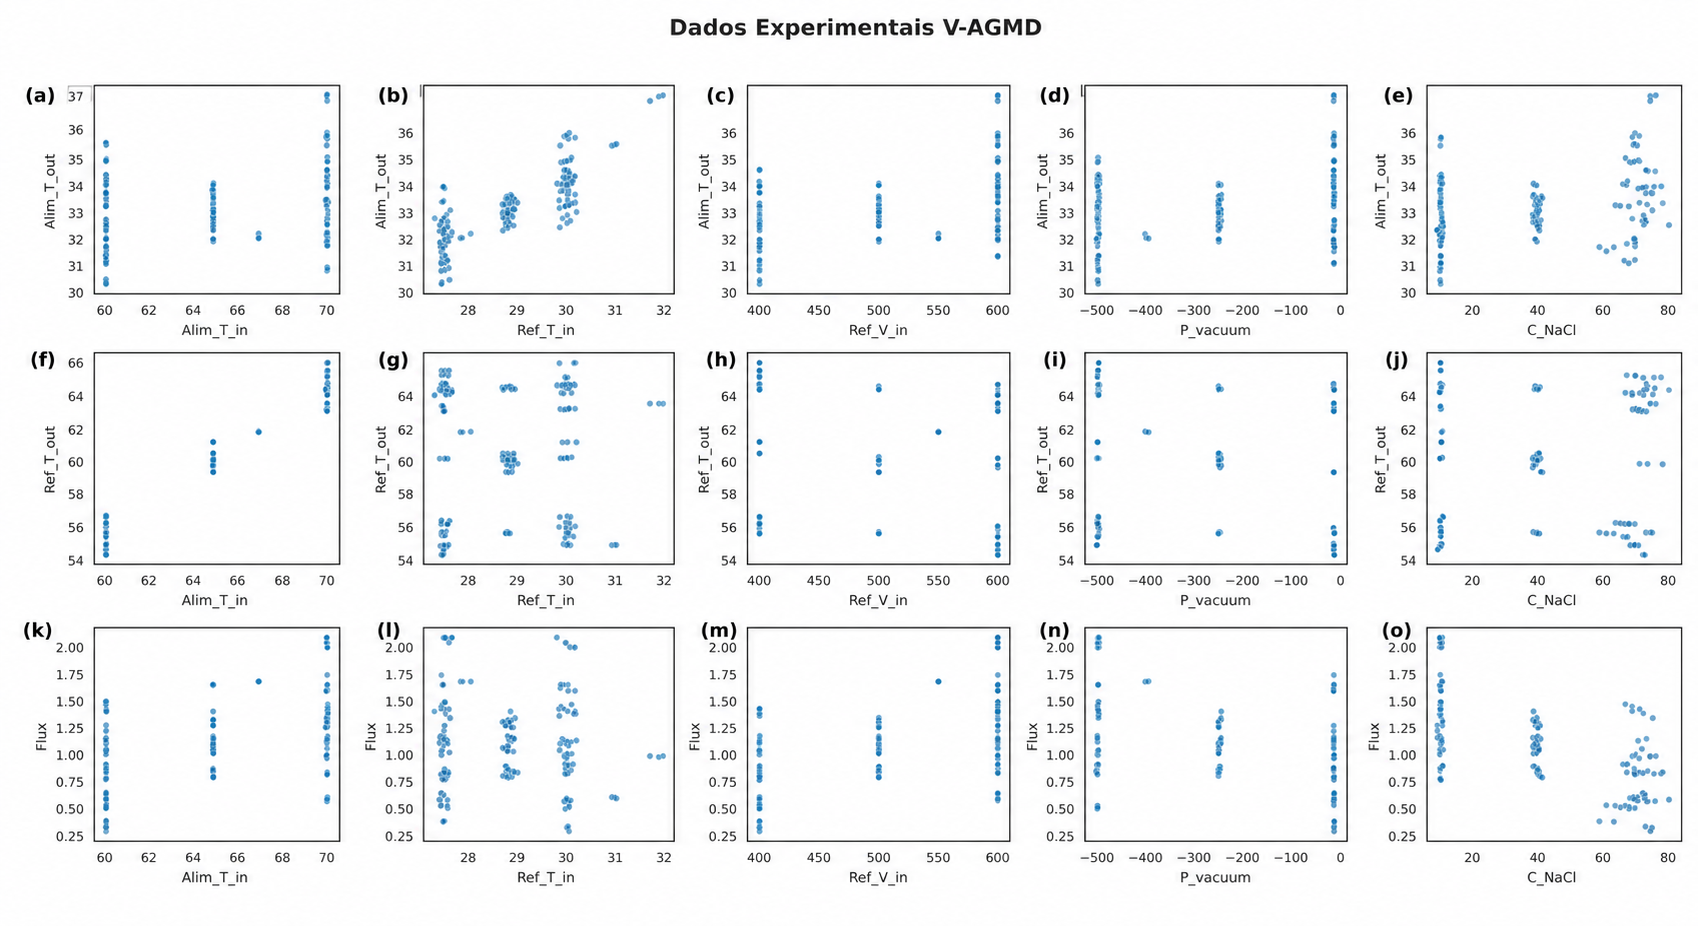
\includegraphics[angle=90, width=0.85\linewidth]{Imagens/chap06/scatter_vagmd_exp_only.png}
    \caption[Dispersão entre variáveis de entrada e saída do sistema V-AGMD]{Gráficos de dispersão entre as variáveis de entrada e as variáveis de saída experimentais do sistema V-AGMD. Fonte: Elaborado pela autora.}
    \label{fig:scatter_vagmd}
\end{figure}
\section{Análise de correlação entre variáveis de entrada e saída}
\label{subsec:correlacao_features_targets}

Com o objetivo de complementar a análise visual preliminar dos dados crus, foram calculados os coeficientes de correlação de Pearson e de Spearman entre as variáveis de entrada e as variáveis de saída do sistema. Conforme discutido na Fundamentação Teórica, esses coeficientes permitem avaliar diferentes formas de associação estatística entre variáveis, sem que isso implique uma relação causal direta entre elas.

Nesta etapa, a análise foi utilizada apenas como ferramenta exploratória, buscando identificar quais variáveis operacionais apresentam maior associação com cada resposta do sistema. A comparação entre os coeficientes de Pearson e Spearman também permite verificar se as associações observadas são mais compatíveis com uma tendência aproximadamente linear ou com uma tendência monotônica mais geral. Assim, os resultados obtidos servem como apoio à interpretação inicial dos dados e à discussão posterior do desempenho dos modelos preditivos.

A Figura~\ref{fig:heatmap_pearson_features_targets} apresenta o mapa de correlação dos coeficientes de correlação de Pearson entre as variáveis de entrada e os alvos. Observa-se que as temperaturas de saída, $Alim\_T_{out}$ e $Ref\_T_{out}$, exibem correlações lineares fortes com variáveis térmicas específicas. No caso das variáveis térmicas, observa-se que as maiores correlações ocorrem entre temperaturas de entrada e saída associadas às correntes que participam diretamente da troca de calor no módulo. Em particular, \(T_{\mathrm{out,alim}}\) (\textit{Alim\_T\_out}) apresenta correlação positiva elevada com a temperatura de entrada da corrente de arrefecimento, \(T_{\mathrm{in,ref}}\) (\textit{Ref\_T\_in}), indicando que o nível térmico da corrente fria influencia a temperatura final da alimentação após a passagem pelo módulo. De forma análoga, \(T_{\mathrm{out,ref}}\) (\textit{Ref\_T\_out}) apresenta correlação positiva elevada com a temperatura de entrada da alimentação, \(T_{\mathrm{in,alim}}\) (\textit{Alim\_T\_in}). Esse comportamento é coerente com a transferência de calor interna ao módulo, na qual parte da energia térmica da corrente de alimentação é transferida para a corrente de arrefecimento, tanto por condução através das camadas do sistema quanto pelo calor associado ao vapor d'água que permeia e condensa. Consequentemente, temperaturas mais elevadas da alimentação tendem a contribuir para maiores temperaturas de saída da corrente de arrefecimento.

\begin{figure}[H]
    \centering
    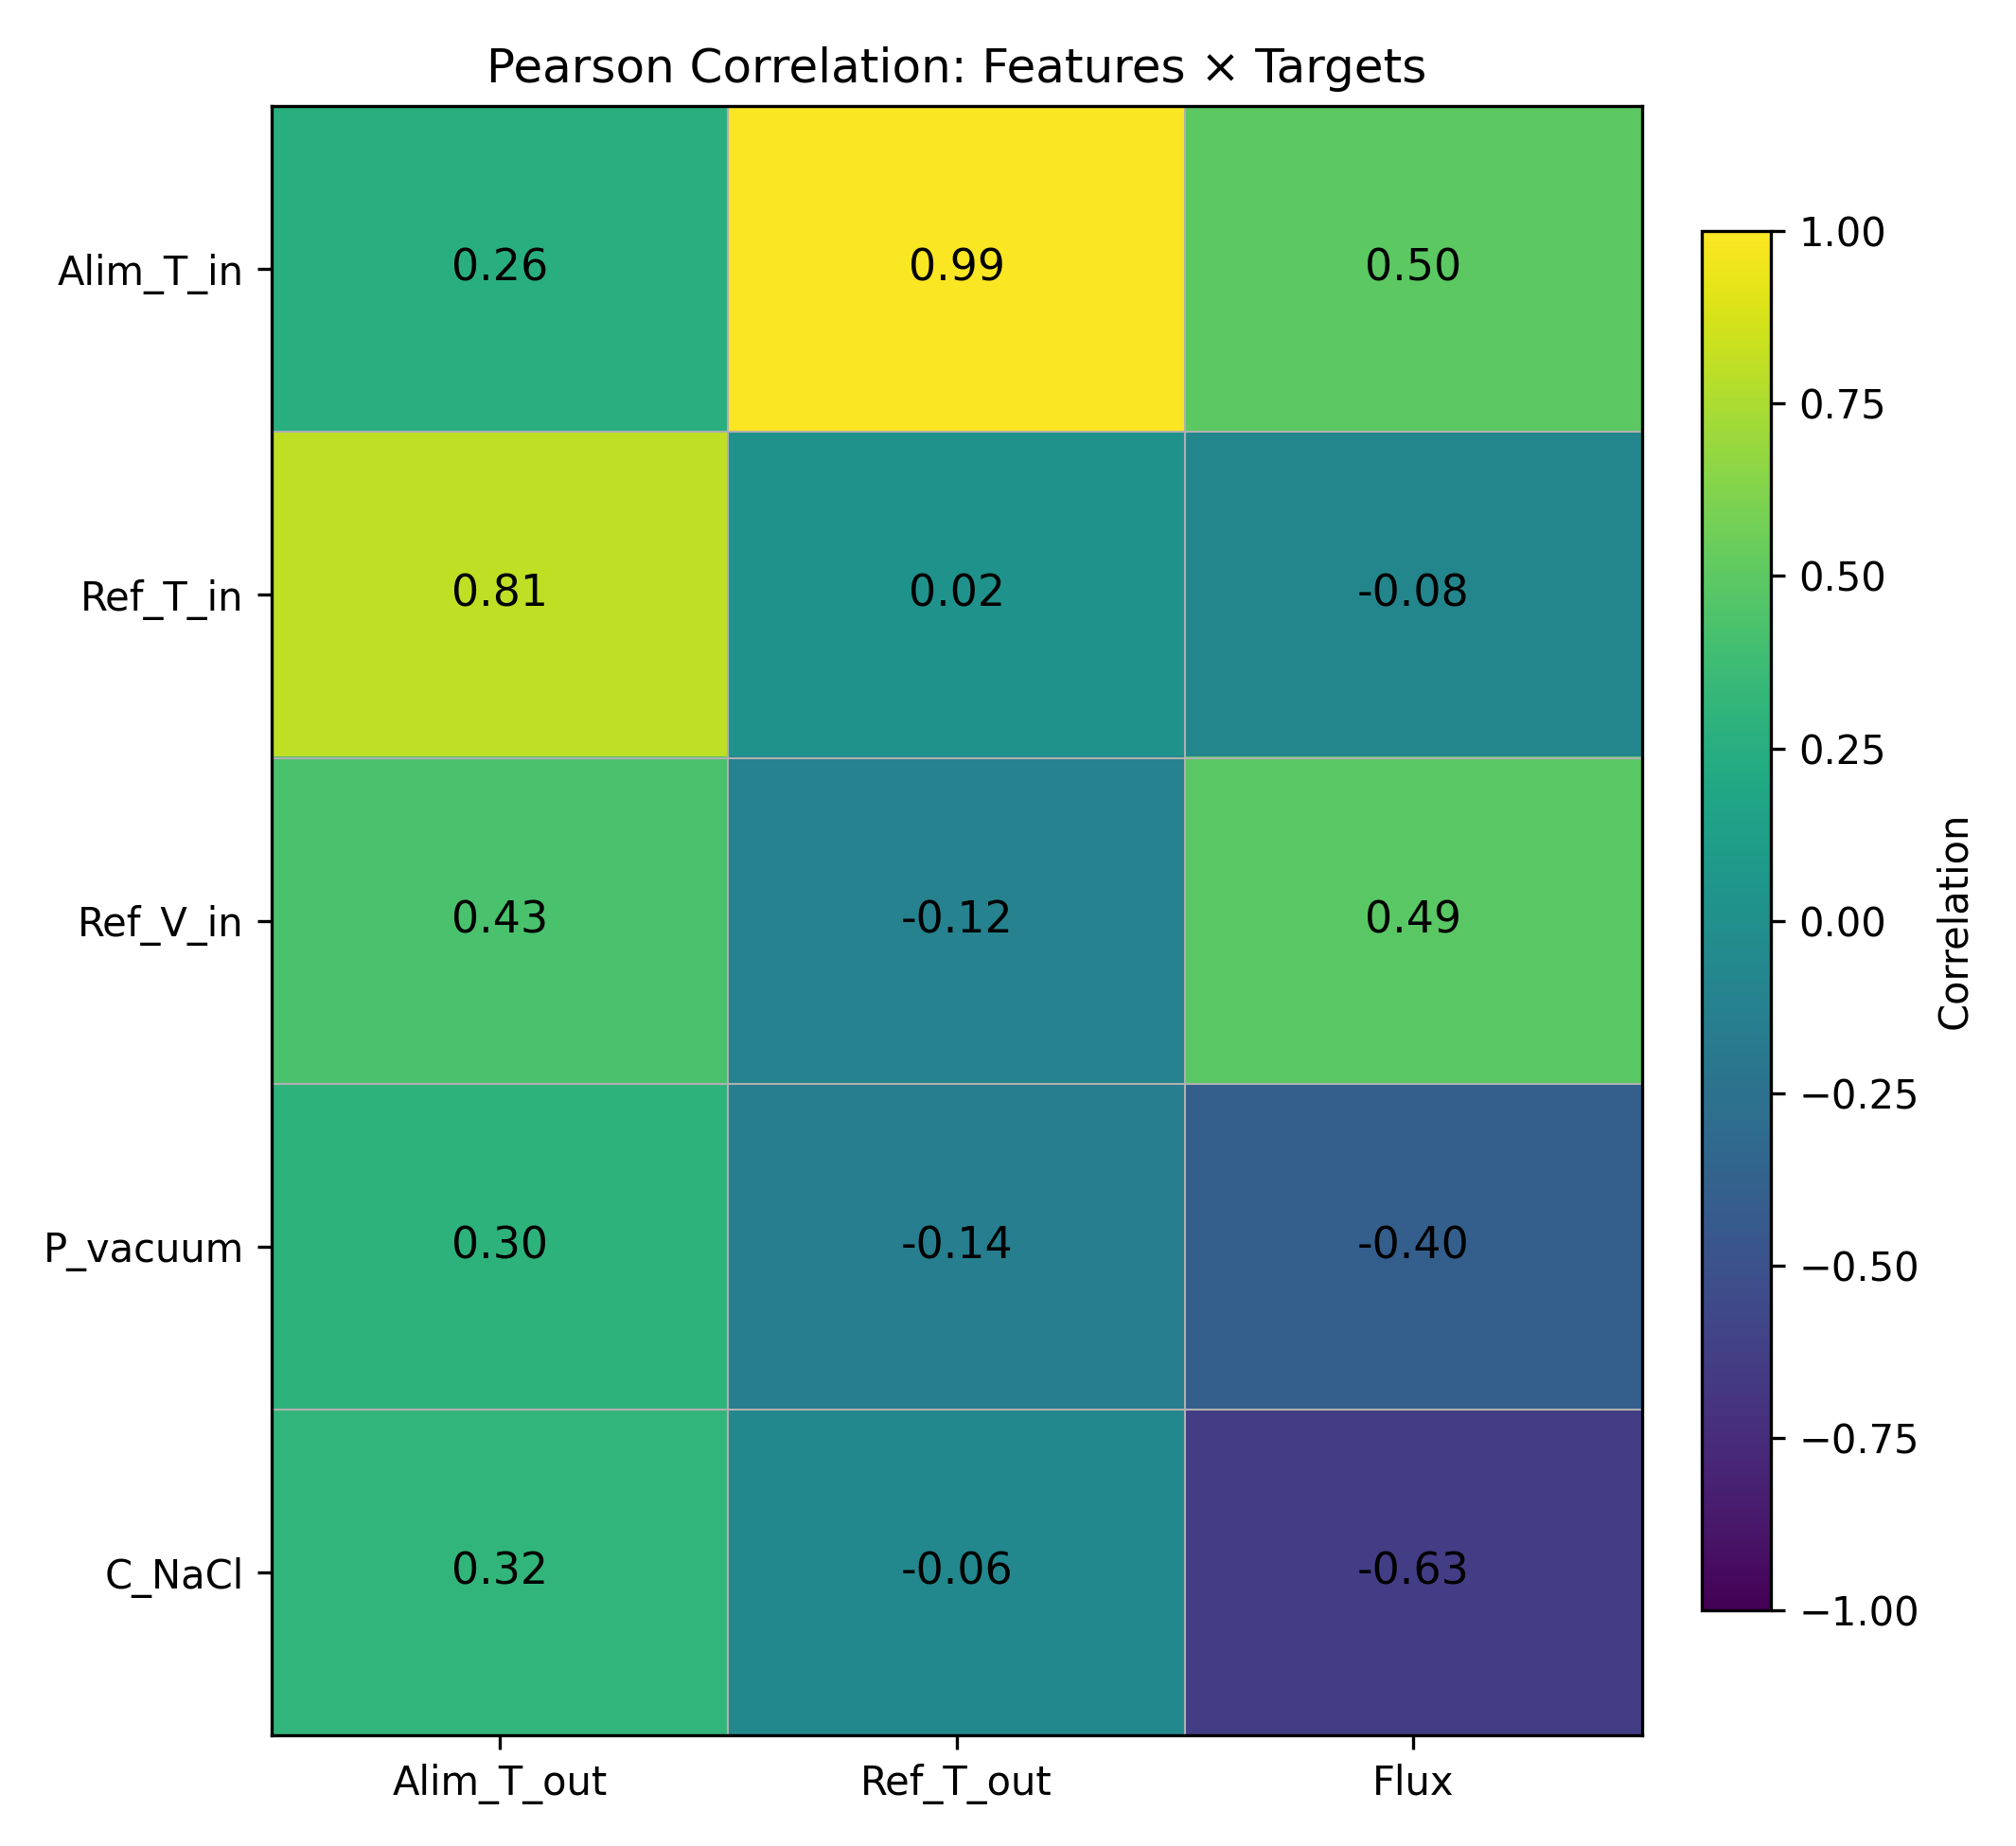
\includegraphics[width=0.9\textwidth]{Imagens/chap06/heatmap_pearson_features_targets.png}
    \caption[Correlação de Pearson entre variáveis do sistema]{Mapa de calor dos coeficientes de correlação de Pearson entre as variáveis de entrada e as variáveis de saída do sistema, utilizado para identificar possíveis relações lineares entre os parâmetros operacionais e as variáveis de desempenho do processo. Fonte: Autor.}
    \label{fig:heatmap_pearson_features_targets}
\end{figure}

Para o fluxo de permeado ($Flux$), a análise de Pearson indica apenas correlações lineares moderadas com variáveis individuais, destacando-se a correlação negativa com a concentração de sal ($C_{NaCl}$) e com a pressão de vácuo ($P_{vac}$), bem como correlações positivas moderadas com a temperatura de alimentação ($Alim\_T_{in}$) e a vazão da solução salina ($\dot{V}_{ref}$). A ausência de correlações lineares fortes sugere que o comportamento do fluxo não é dominado por uma única variável de entrada quando analisado de forma isolada.

A Figura~5.3 apresenta o mapa de correlação correspondente aos coeficientes de correlação de Spearman. De modo geral, observa-se que, para as temperaturas de saída, os valores de Spearman são próximos aos de Pearson, indicando que as relações dominantes são não apenas monotônicas, mas também aproximadamente lineares no domínio experimental considerado. Esse resultado é coerente com a interpretação física discutida anteriormente, segundo a qual as temperaturas de saída são fortemente influenciadas pela troca de calor entre a corrente de alimentação e a corrente de arrefecimento no interior do módulo. Em particular, o aumento da temperatura de entrada de uma corrente tende a afetar a temperatura de saída da outra, devido à transferência de energia térmica por condução através das camadas do sistema e pelo calor associado ao vapor d'água que permeia e condensa.

Os gráficos de dispersão foram mantidos como etapa qualitativa preliminar por evidenciarem a estrutura discreta do planejamento experimental e a sobreposição de efeitos entre variáveis operacionais. No entanto, a interpretação quantitativa das associações foi conduzida principalmente a partir dos mapas de correlação.

\begin{figure}[H]
    \centering
    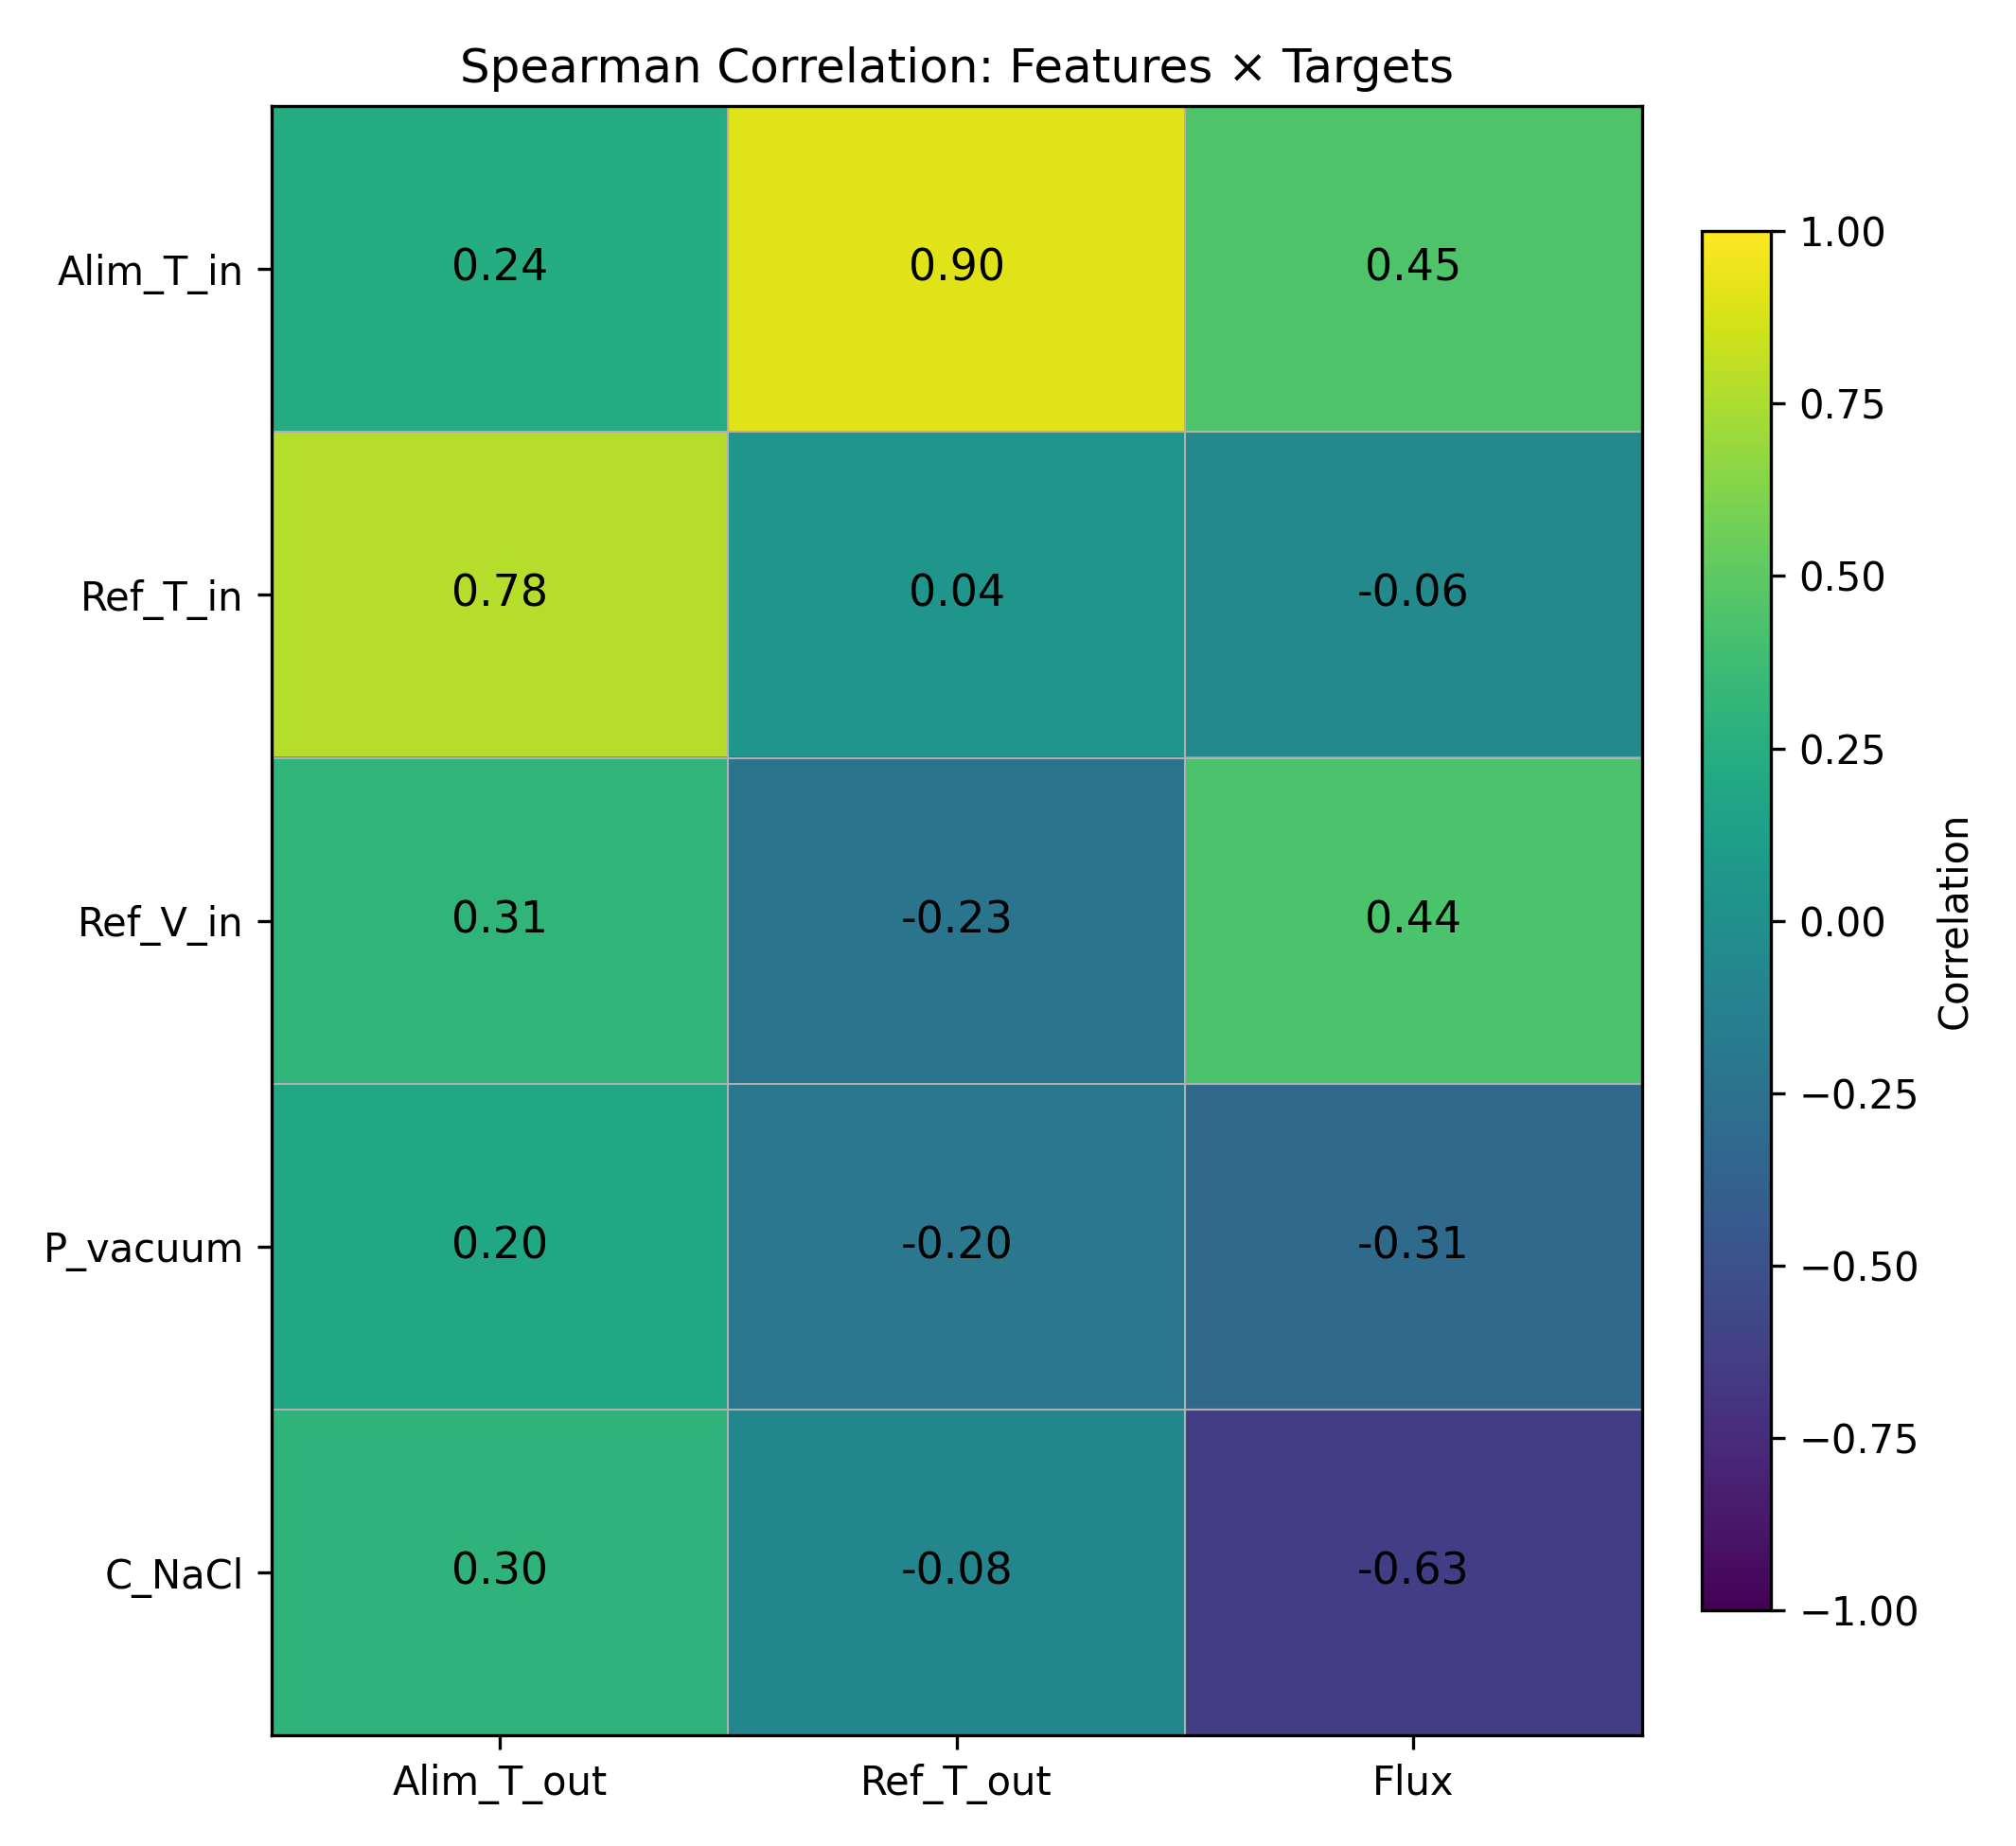
\includegraphics[width=0.9\textwidth]{Imagens/chap06/heatmap_spearman_features_targets.png}
    \caption[Correlação de Spearman entre variáveis do sistema]{Mapa de calor dos coeficientes de correlação de Spearman entre as variáveis de entrada e as variáveis de saída do sistema, utilizado para identificar relações monotônicas entre os parâmetros operacionais e as variáveis de desempenho do processo. Fonte: Autor.}
    \label{fig:heatmap_spearman_features_targets}
\end{figure}

No caso do fluxo de permeado, a proximidade entre os coeficientes de Pearson e de Spearman indica que as relações entre o fluxo e as variáveis operacionais são predominantemente monotônicas, porém distribuídas entre múltiplas variáveis, sem evidência de não linearidades marginais pronunciadas quando cada entrada é considerada isoladamente. Esse comportamento sugere que a complexidade do fluxo decorre principalmente de interações multivariadas entre condições operacionais, o que limita a interpretação baseada exclusivamente em correlações univariadas.

Em conjunto, os mapas de correlação reforçam as conclusões da análise visual preliminar: as temperaturas de saída apresentam comportamento fortemente governado por relações lineares dominantes, enquanto o fluxo de permeado não pode ser adequadamente descrito por relações lineares simples com variáveis individuais. Esses resultados motivam análises adicionais baseadas em gráficos de dispersão condicionais e em métodos de validação cruzada, capazes de capturar efeitos de interação e avaliar o impacto dessas relações no desempenho preditivo dos modelos.

\section{Avaliação do desempenho do modelo físico reduzido (0D)}
\label{subsec:avaliacao_modelo_0d}

Antes da aplicação dos modelos orientados por dados, avaliou-se o comportamento do modelo físico reduzido (0D) utilizado como referência fenomenológica neste trabalho. O objetivo desta análise não foi recalibrar ou propor modificações ao modelo físico, mas verificar como suas estimativas se comportam quando aplicadas às condições experimentais disponíveis e em que medida elas reproduzem as variáveis de saída de interesse.

O modelo 0D foi executado a partir das variáveis operacionais medidas experimentalmente: temperatura de entrada da alimentação \(T_{\mathrm{in,alim}}\), temperatura de entrada da corrente de arrefecimento \(T_{\mathrm{in,ref}}\), vazão volumétrica da solução salina \(\dot{V}_{\mathrm{in}}\), pressão manométrica na câmara de ar \(P_{\mathrm{man}}\) e concentração de NaCl \(C_{\mathrm{NaCl}}\). As saídas calculadas pelo modelo físico foram então comparadas com os valores experimentais correspondentes de temperatura de saída da alimentação, temperatura de saída da corrente de arrefecimento e fluxo de permeado.

Inicialmente, realizou-se uma verificação preliminar utilizando os dados experimentais reportados no trabalho em que o modelo físico reduzido foi originalmente proposto (\cite{Lisboa2024}). Essa etapa teve como finalidade apenas verificar a consistência da aplicação local do código em C disponibilizado, incluindo a leitura das variáveis de entrada, as conversões de unidades necessárias e a extração das saídas calculadas. Portanto, essa verificação não corresponde a uma nova validação do modelo físico, mas a uma etapa de controle antes de sua aplicação ao conjunto de dados experimental utilizado neste trabalho.

A Figura~\ref{fig:flux_article_vs_exp} apresenta a comparação entre o fluxo de permeado experimental e o fluxo de permeado calculado pelo modelo 0D. Em \ref{fig:flux_article_vs_exp}(a), são utilizados os dados experimentais reportados na literatura; em \ref{fig:flux_article_vs_exp}(b), são utilizados os dados experimentais deste trabalho. Em ambos os casos, a linha diagonal representa a concordância ideal entre o valor experimental e o valor calculado pelo modelo.

\begin{figure}[H]
    \centering
    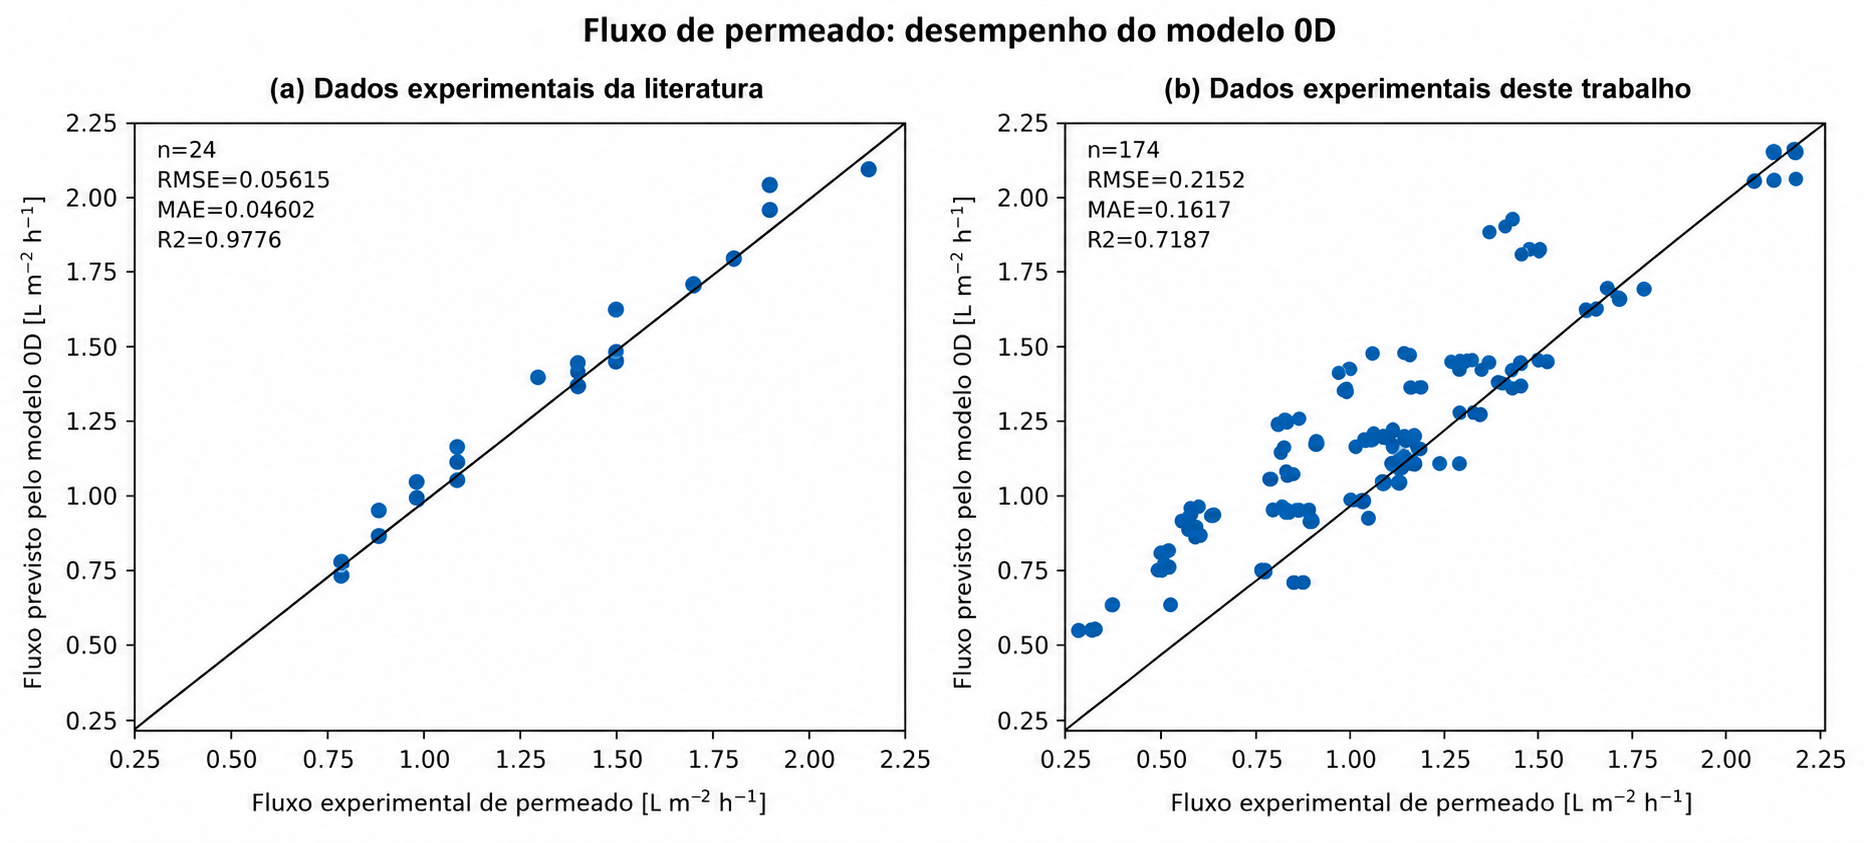
\includegraphics[width=0.9\linewidth]{Imagens/chap06/compare_flux_0d.png}
    \caption[Desempenho do modelo físico 0D na predição do fluxo de permeado]{Comparação entre o fluxo de permeado experimental e o fluxo de permeado calculado pelo modelo físico reduzido (0D). Em (a), são apresentados os dados experimentais reportados na literatura; em (b), são apresentados os dados experimentais deste trabalho. A linha diagonal indica a concordância ideal entre valores experimentais e calculados pelo modelo.}
    \fonte{Elaborado pela autora.}
    \label{fig:flux_article_vs_exp}
\end{figure}

% Após a atualização da figura, acrescentar na legenda:
% As barras de erro representam a incerteza associada às medidas experimentais de fluxo.

Observa-se que, para os dados experimentais da literatura, os pontos se distribuem próximos à reta de concordância, indicando que a execução local do modelo reproduz de forma consistente o comportamento reportado para o conjunto de dados usado como referência. Esse resultado é importante porque confirma que o procedimento computacional adotado neste trabalho está coerente com a formulação original do modelo físico.

Quando o modelo é aplicado aos dados experimentais deste trabalho, entretanto, observa-se maior dispersão em relação à reta identidade. Esse comportamento indica que o modelo 0D ainda acompanha a tendência global do fluxo de permeado, mas não reproduz integralmente a variabilidade observada no novo conjunto experimental. Essa diferença pode estar associada tanto às condições operacionais específicas avaliadas neste trabalho quanto às simplificações inerentes à formulação reduzida do modelo, que representa o módulo de forma concentrada e não descreve explicitamente variações espaciais ao longo dos canais.

Além da comparação para o fluxo de permeado, também foram avaliadas as demais variáveis de saída consideradas no problema de regressão. As Figuras~\ref{fig:alim_t_out_0d}, \ref{fig:ref_t_out_0d} e \ref{fig:flux_0d_exp} apresentam, respectivamente, as comparações entre valores experimentais e valores calculados pelo modelo 0D para a temperatura de saída da alimentação, a temperatura de saída da corrente de arrefecimento e o fluxo de permeado.

\begin{figure}[H]
    \centering
    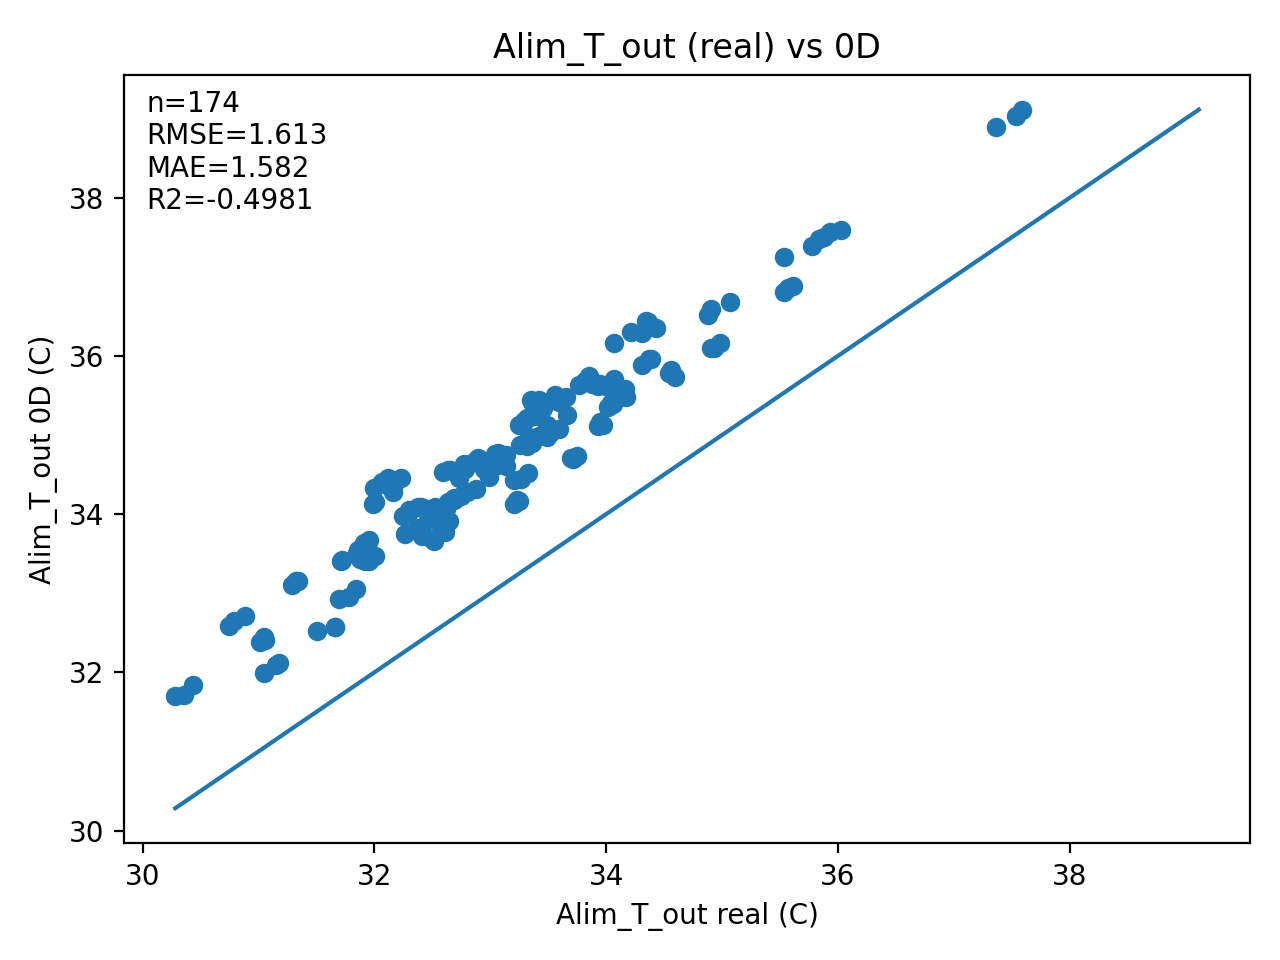
\includegraphics[width=0.7\linewidth]{Imagens/chap06/alim_T_out_real_vs_0d.png}
    \caption[Predição da temperatura de saída da alimentação pelo modelo 0D]{Comparação entre a temperatura de saída da alimentação medida experimentalmente e a temperatura calculada pelo modelo físico reduzido (0D). A linha diagonal indica a concordância ideal entre valores experimentais e calculados pelo modelo.}
    \fonte{Elaborado pela autora.}
    \label{fig:alim_t_out_0d}
\end{figure}

\begin{figure}[H]
    \centering
    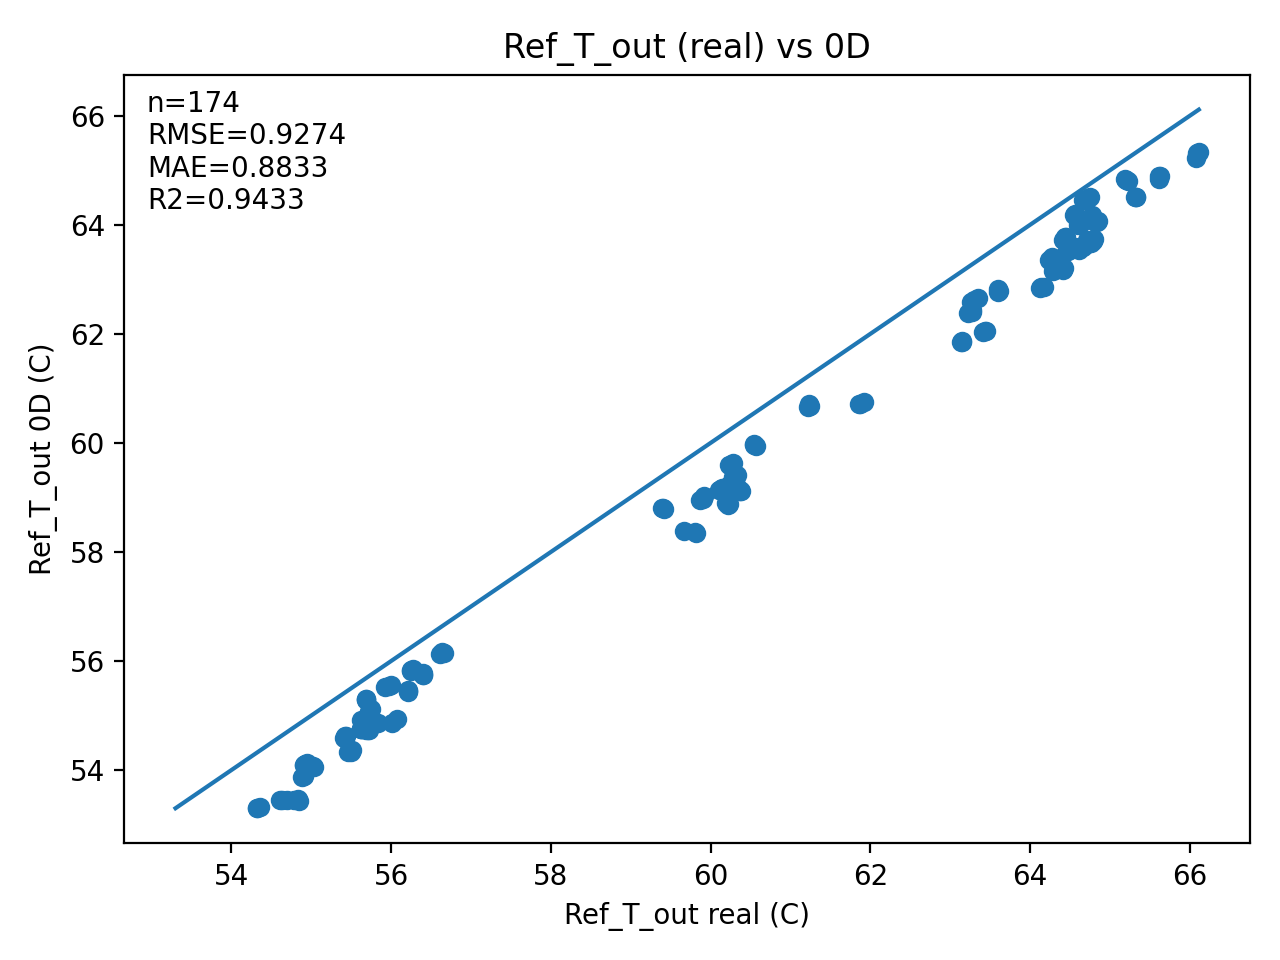
\includegraphics[width=0.7\linewidth]{Imagens/chap06/ref_T_out_real_vs_0d.png}
    \caption[Predição da temperatura de saída da corrente de arrefecimento pelo modelo 0D]{Comparação entre a temperatura de saída da corrente de arrefecimento medida experimentalmente e a temperatura calculada pelo modelo físico reduzido (0D). A linha diagonal indica a concordância ideal entre valores experimentais e calculados pelo modelo.}
    \fonte{Elaborado pela autora.}
    \label{fig:ref_t_out_0d}
\end{figure}

\begin{figure}[H]
    \centering
    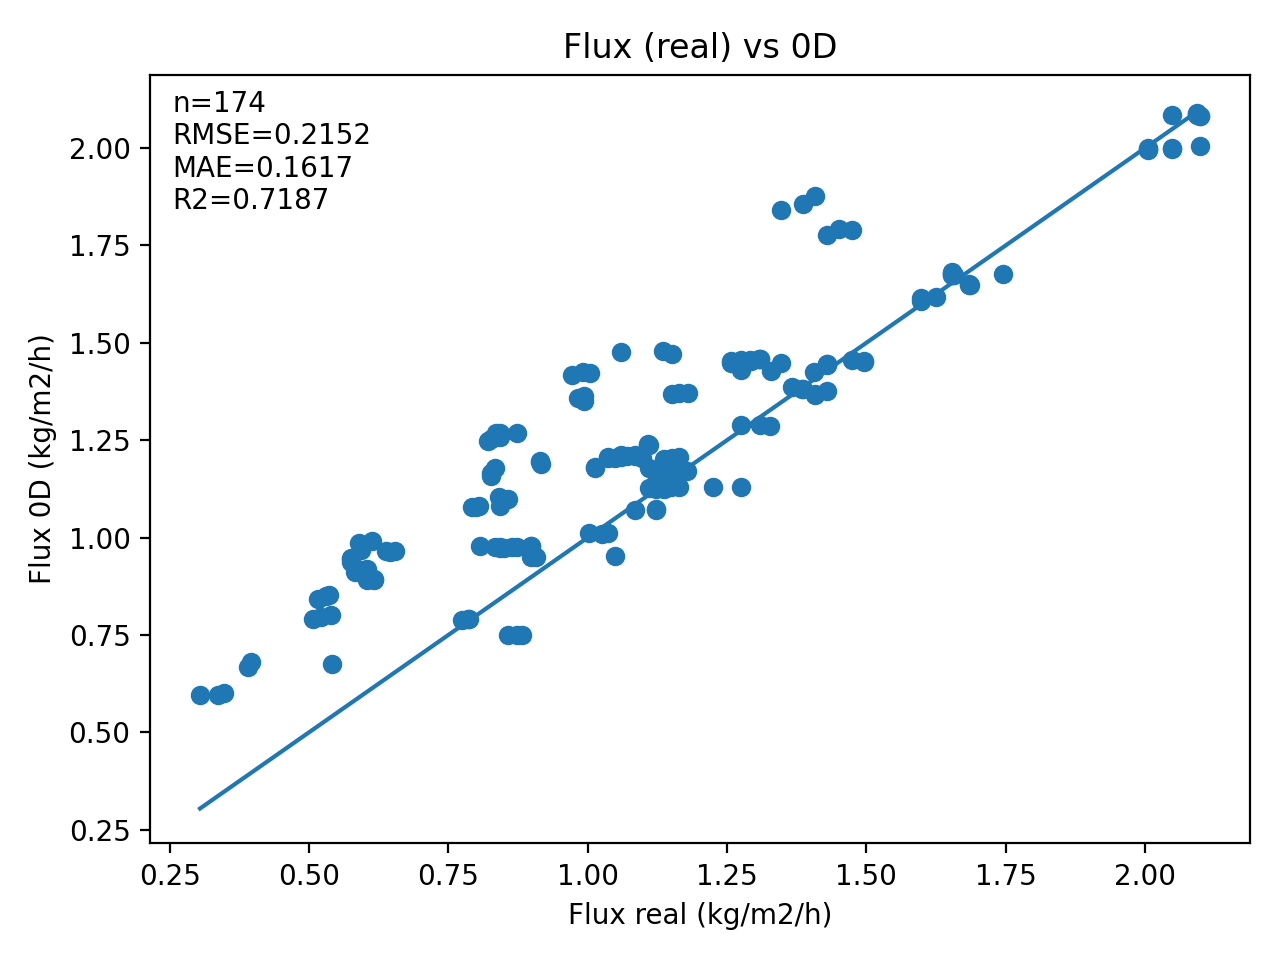
\includegraphics[width=0.7\linewidth]{Imagens/chap06/flux_real_vs_0d.png}
    \caption[Predição do fluxo de permeado pelo modelo 0D]{Comparação entre o fluxo de permeado medido experimentalmente e o fluxo calculado pelo modelo físico reduzido (0D). A linha diagonal indica a concordância ideal entre valores experimentais e calculados pelo modelo.}
    \fonte{Elaborado pela autora.}
    \label{fig:flux_0d_exp}
\end{figure}

A análise conjunta dessas três variáveis mostra que o desempenho do modelo 0D não é uniforme para todas as saídas. A melhor aderência ocorre para \(T_{\mathrm{out,ref}}\), sugerindo que o modelo representa de forma mais adequada a resposta térmica da corrente de arrefecimento. Esse resultado é coerente com a estrutura do modelo físico, que descreve diretamente os balanços de energia associados à transferência de calor entre as correntes no interior do módulo.

Para o fluxo de permeado, o comportamento é intermediário. O modelo acompanha a tendência geral dos dados, mas apresenta dispersão mais elevada em relação à reta de concordância. Isso indica que a formulação reduzida captura parte dos efeitos físicos dominantes associados à transferência de massa, mas não descreve completamente a variabilidade experimental do fluxo. Essa limitação é esperada, uma vez que o fluxo depende de fenômenos acoplados de transferência de calor e massa, incluindo diferenças locais de temperatura, pressão parcial de vapor, salinidade e condições de escoamento.

Já para \(T_{\mathrm{out,alim}}\), observa-se maior viés sistemático, indicando que o modelo tende a se afastar de forma mais consistente dos valores experimentais. Esse comportamento sugere que a temperatura de saída da alimentação é mais sensível a efeitos não capturados integralmente pela formulação 0D, como variações espaciais de temperatura ao longo do canal, perdas térmicas, heterogeneidades no escoamento ou simplificações nas resistências térmicas adotadas.

Portanto, a avaliação do modelo 0D cumpre dois papéis nesta etapa do trabalho. Primeiro, ela mostra que o modelo físico constitui uma referência fenomenológica relevante, capaz de representar tendências gerais do sistema e de fornecer estimativas fisicamente interpretáveis. Segundo, evidencia que essas estimativas não reproduzem integralmente os dados experimentais deste trabalho, especialmente para o fluxo de permeado e para a temperatura de saída da alimentação. Essa constatação justifica a investigação posterior de modelos orientados por dados e de estratégias híbridas físico--dados, nas quais as previsões do modelo 0D são utilizadas como informação auxiliar, mas combinadas à capacidade de ajuste dos métodos de aprendizado de máquina.
\section{Avaliação comparativa dos pipelines baseados em dados}
\label{subsec:avaliacao_pipelines_dados}

Após a avaliação do modelo físico reduzido, investigou-se o desempenho de modelos orientados por dados para a predição simultânea das três variáveis de saída consideradas neste trabalho: temperatura de saída da alimentação ($Alim\_T_{out}$), temperatura de saída do circuito de referência ($Ref\_T_{out}$) e fluxo de permeado ($Flux$). O objetivo dessa etapa não foi apenas comparar diferentes famílias de modelos, mas também estabelecer um \textit{pipeline} de modelagem compatível com as características do conjunto de dados experimental disponível.

Inicialmente, foram examinadas duas diferentes estratégias de pré-processamento, incluindo a utilização direta dos dados experimentais e a discretização de variáveis de entrada por meio de \textit{binning}. As análises preliminares indicaram, entretanto, que a abordagem de discretização não produziu ganhos consistentes de desempenho ou generalização no problema estudado. Dessa forma, a etapa completa de seleção e comparação entre modelos foi conduzida utilizando apenas o pipeline baseado nos dados experimentais originais.

\subsection{Estratégia de análise dos resultados}
\label{subsubsec:estrategia_validacao}

Os resultados apresentados nesta seção foram obtidos a partir do procedimento de validação cruzada agrupada por \textit{Regime} e do critério hierárquico de seleção descritos no Capítulo de Metodologia. Portanto, os detalhes do particionamento dos dados, da busca de hiperparâmetros e da regra de seleção não são retomados aqui. A presente seção concentra-se na interpretação comparativa do desempenho dos modelos selecionados em cada família.

A análise foi conduzida tomando o fluxo de permeado como variável prioritária de comparação, pois essa grandeza representa diretamente a produtividade do processo V-AGMD. Em outras palavras, a escolha das configurações foi orientada principalmente pela capacidade de prever a taxa de produção de permeado por área de membrana, que é o indicador mais diretamente associado ao desempenho operacional do sistema. As temperaturas de saída também foram avaliadas, mas como variáveis complementares para verificar se a priorização do fluxo comprometia a representação do comportamento térmico do módulo.

Dessa forma, a discussão dos resultados é organizada em três etapas. Primeiro, compara-se o desempenho global das famílias de modelos com base no RMSE do fluxo de permeado. Em seguida, avalia-se o comportamento dos modelos selecionados para as três variáveis de saída, permitindo verificar a qualidade preditiva de forma conjunta. Por fim, são analisados os gráficos de valores preditos em função dos valores experimentais, com o objetivo de identificar padrões de aderência, dispersão e possíveis vieses nas previsões.
\subsection{Comparação global entre modelos}

A comparação global entre modelos tem como objetivo avaliar, de forma integrada, o desempenho das diferentes abordagens testadas no \textit{pipeline} de modelagem. A escolha dos modelos não foi conduzida apenas por tentativa e erro, mas organizada de forma progressiva para comparar alternativas com diferentes níveis de complexidade, capacidade de representação não linear e incorporação de conhecimento físico.

Para isso, os modelos foram agrupados em três classes principais: modelos clássicos de regressão, redes neurais puramente orientadas por dados e estratégias híbridas físico--dados. A Tabela~\ref{tab:familias_modelos_avaliados} resume o papel de cada grupo no processo de comparação.

\begin{table}[H]
\centering
\caption{Síntese das famílias de modelos avaliadas no \textit{pipeline}.}
\label{tab:familias_modelos_avaliados}
\small
\begin{tabular}{p{0.20\textwidth}p{0.28\textwidth}p{0.27\textwidth}p{0.17\textwidth}}
\toprule
Família de modelos & Modelos avaliados & Papel na comparação & Característica principal \\
\midrule
Modelos lineares clássicos & OLS, Ridge, Lasso e ElasticNet, incluindo formulações multitarefa e independentes & Servem como referência de menor complexidade para verificar se relações mais simples já descrevem parte do comportamento observado & Baixa complexidade e maior interpretabilidade \\
\midrule
Modelos baseados em árvores & Árvore de decisão, floresta aleatória e \textit{Gradient Boosting} & Avaliam se partições não lineares do espaço de entrada melhoram a predição em relação aos modelos lineares & Maior flexibilidade, com possível sensibilidade aos dados de treinamento \\
\midrule
Redes neurais puramente orientadas por dados & MLP e rede neural de referência & Avaliam se uma arquitetura neural, sem incorporação explícita de informação física, é suficiente para capturar relações não lineares entre entradas e saídas & Capacidade de aproximação não linear \\
\midrule
Modelos híbridos físico--dados & ZohanResidual, ZohanHPD, Luc e FrozenBaseline & Avaliam se a incorporação de informação proveniente do modelo físico reduzido melhora a predição em relação às abordagens puramente orientadas por dados & Combinação entre tendência física e correção aprendida por dados \\
\bottomrule
\end{tabular}
\end{table}

Todos os modelos e configurações foram avaliados sob o mesmo procedimento de validação cruzada agrupada por \textit{Regime}, conforme descrito na Metodologia. Dessa forma, as diferenças observadas no desempenho não refletem apenas a capacidade de ajuste aos dados de treinamento, mas também a capacidade dos modelos de generalizar para regimes experimentais mantidos fora do treinamento em cada partição da validação cruzada.

A leitura dos resultados desta seção deve considerar três aspectos principais. Primeiro, como o fluxo de permeado foi definido como variável prioritária de seleção, o desempenho em $Flux$ é o critério central para escolha do modelo final. Segundo, como o problema é multi-saída, é necessário verificar se o bom desempenho no fluxo é acompanhado por resultados adequados nas temperaturas de saída, $T_{\mathrm{alim,out}}$ e $T_{\mathrm{ref,out}}$. Terceiro, a comparação entre famílias permite avaliar se o ganho obtido decorre apenas do aumento de flexibilidade do modelo ou se a incorporação de informação física trouxe benefício adicional.

Nesse sentido, a Tabela~\ref{tab:model_performance_outputs} consolida os valores de RMSE e $R^2$ para as três variáveis de saída. Os valores reportados correspondem às métricas calculadas a partir das predições \textit{out-of-fold} (OOF), conforme descrito na Seção~\ref{sec:avaliacao_oof}. Diferentemente do RMSE médio de validação cruzada utilizado durante a seleção de hiperparâmetros, as métricas OOF são obtidas a partir de modelos retreinados independentemente em cada partição, reduzindo o viés de otimismo associado ao processo de seleção (\cite{Cawley2010Overfitting}). A linha destacada corresponde ao modelo híbrido ZohanResidual, selecionado como modelo final.

\begin{table}[H]
\centering
\caption[Desempenho OOF consolidado dos modelos avaliados]{Desempenho consolidado dos modelos avaliados com base nas predições \textit{out-of-fold} (OOF), ordenados pelo RMSE do fluxo de permeado. As métricas OOF são calculadas sobre predições de modelos retreinados independentemente em cada partição da validação cruzada (\cite{Cawley2010Overfitting}). A linha destacada corresponde ao modelo final selecionado.}
\label{tab:model_performance_outputs}
\begin{tabular}{l c c c c c c}
\toprule
\multirow{2}{*}{Modelo} & \multicolumn{2}{c}{\textbf{$Alim\_T_{out}$}} & \multicolumn{2}{c}{\textbf{$Ref\_T_{out}$}} & \multicolumn{2}{c}{\textbf{$Flux$}} \\
\cmidrule(lr){2-3} \cmidrule(lr){4-5} \cmidrule(lr){6-7}
 & R$^2$ & RMSE & R$^2$ & RMSE & R$^2$ & RMSE \\
\midrule
\multicolumn{7}{c}{\textbf{Modelos clássicos}} \\
\midrule
MLP\_sklearn & 0.922 & 0.368 & 0.925 & 1.067 & 0.970 & 0.071 \\
OLS & 0.965 & 0.246 & 0.996 & 0.251 & 0.952 & 0.089 \\
Lasso & 0.965 & 0.245 & 0.996 & 0.251 & 0.951 & 0.090 \\
Ridge & 0.962 & 0.257 & 0.989 & 0.401 & 0.938 & 0.101 \\
\midrule
\multicolumn{7}{c}{\textbf{Modelos híbridos}} \\
\midrule
\rowcolor{orange!15}
ZohanResidual & 0.951 & 0.290 & 0.990 & 0.385 & \textbf{0.978} & \textbf{0.061} \\
HRNN & 0.972 & 0.221 & 0.991 & 0.377 & 0.963 & 0.078 \\
Luc & 0.931 & 0.347 & 0.985 & 0.482 & 0.954 & 0.087 \\
FrozenBaseline & 0.968 & 0.237 & 0.990 & 0.394 & 0.949 & 0.091 \\
\midrule
\multicolumn{7}{c}{\textbf{Modelo físico de referência}} \\
\midrule
Modelo físico 0D & -0.498 & 1.613 & 0.943 & 0.927 & 0.719 & 0.215 \\
\bottomrule
\end{tabular}
\end{table}

A partir da Tabela~\ref{tab:model_performance_outputs}, observa-se que o modelo híbrido ZohanResidual apresentou a melhor combinação global de desempenho. Para o alvo prioritário $Flux$, esse modelo obteve o menor RMSE (0,061) e o maior R² (0,978) entre as configurações avaliadas, representando uma redução de 33\% no RMSE em relação ao modelo puramente orientado por dados (FrozenBaseline, RMSE 0,091). Esse ganho evidencia que a incorporação da informação física, por meio da arquitetura residual, permitiu ao modelo aprender correções mais precisas para a predição do fluxo de permeado.

O modelo HRNN, que utiliza a arquitetura residual com concatenação total das entradas, também apresentou ganho significativo, com RMSE de 0,078 e R² de 0,963. O modelo Luc, que utiliza regularização física na função de perda, apresentou desempenho intermediário (RMSE 0,087), enquanto o FrozenBaseline, puramente orientado por dados, obteve RMSE de 0,091. Esses resultados indicam que a estratégia de incorporação da física influencia diretamente o ganho preditivo: a abordagem residual (ZohanResidual) mostrou-se mais eficaz do que a regularização na perda (Luc) para o problema em questão.

Para complementar a leitura da Tabela~\ref{tab:model_performance_outputs}, a Figura~\ref{fig:ranking_rmse_targets} apresenta o ranking dos modelos em função do RMSE para cada uma das três variáveis de saída. Diferentemente da figura anterior, que mostrava apenas o fluxo de permeado, esta visualização permite verificar se a ordenação dos modelos se mantém quando são consideradas também as temperaturas de saída. Os nomes dos modelos utilizados na figura são os mesmos adotados na tabela, de modo a facilitar a comparação direta entre as duas representações.

\begin{figure}[H]
\centering
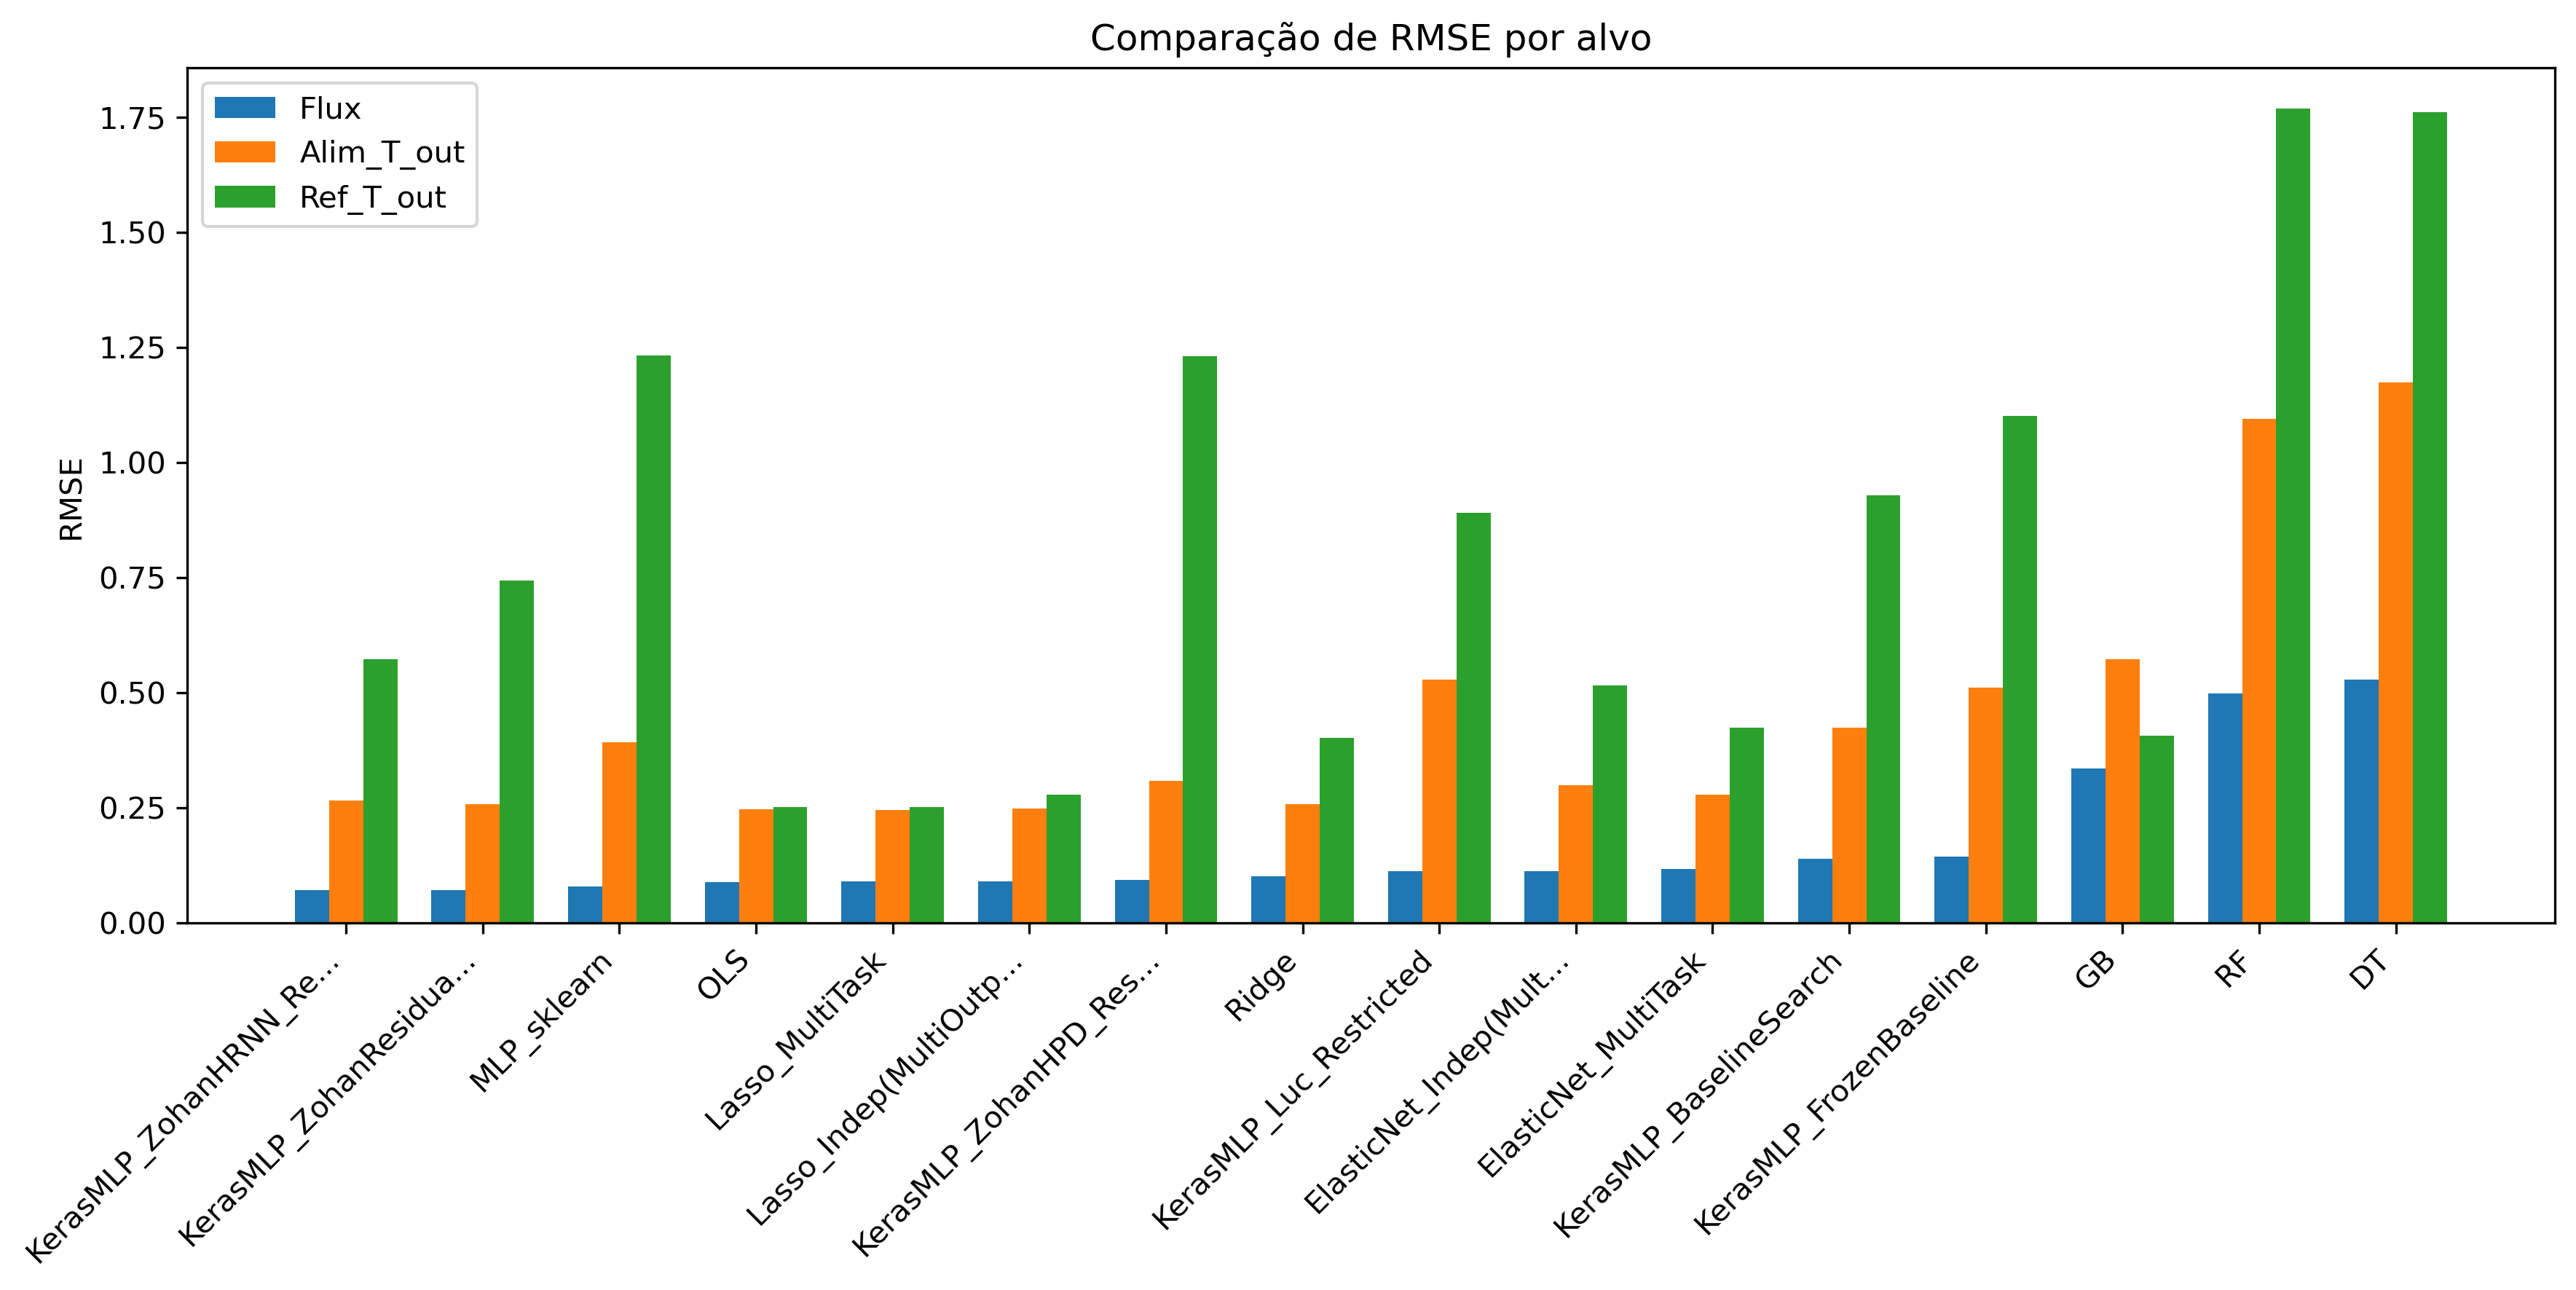
\includegraphics[width=1\textwidth]{Imagens/chap06/rmse_by_target_grouped.png}
\caption[Ranking dos modelos por RMSE para cada variável de saída]{Ranking dos modelos avaliados com base no erro quadrático médio da raiz (RMSE) para cada variável de saída do sistema: fluxo de permeado, temperatura de saída da alimentação e temperatura de saída do circuito de resfriamento. Os nomes dos modelos seguem a mesma nomenclatura apresentada na Tabela~\ref{tab:model_performance_outputs}. Fonte: Autor.}
\label{fig:ranking_rmse_targets}
\end{figure}

A Figura~\ref{fig:ranking_rmse_targets} evidencia que o modelo ZohanResidual permanece entre os melhores modelos nos três alvos avaliados. No caso do $Flux$, sua posição no topo do ranking confirma sua adequação ao critério principal de seleção. Para as temperaturas de saída, o desempenho também se mantém competitivo, com menor RMSE em relação às demais abordagens avaliadas. Esse comportamento reforça que o modelo selecionado não apresentou bom desempenho apenas no alvo priorizado, mas também preservou qualidade preditiva nas demais respostas do sistema.

Dessa forma, os resultados indicam que o modelo mais indicado para o objetivo principal deste trabalho é o modelo híbrido ZohanResidual. Essa escolha não decorre apenas do uso de uma arquitetura mais complexa, mas do ganho preditivo observado para o fluxo de permeado, aliado à incorporação de informação física e à manutenção de desempenho satisfatório para as demais variáveis de saída. Os modelos lineares permanecem relevantes como referências de comparação, pois mostram que parte do comportamento do sistema pode ser descrita por relações mais simples. No entanto, para a finalidade central deste estudo, que é prever o desempenho do processo V-AGMD com foco no fluxo de permeado, a abordagem híbrida apresentou a melhor combinação entre erro, generalização e coerência física.
\subsection{Interpretação física do desempenho dos modelos}
\label{subsec:interpretacao_fisica_modelos}

A análise dos resultados obtidos mostra que o desempenho dos modelos não foi uniforme para todas as variáveis de saída. As temperaturas de saída da alimentação, $T_{\mathrm{alim,out}}$, e do circuito de resfriamento, $T_{\mathrm{ref,out}}$, apresentaram resultados satisfatórios para diferentes famílias de modelos. Já a predição do fluxo de permeado, $Flux$, mostrou maior sensibilidade à escolha da arquitetura de modelagem, sendo o alvo para o qual a abordagem híbrida apresentou ganho mais expressivo.

Esse comportamento deve ser interpretado considerando que, no processo de destilação por membranas, os fenômenos de transferência de calor e massa estão diretamente acoplados. O fluxo de permeado depende dos gradientes térmicos e da diferença de pressão de vapor estabelecida através da membrana, enquanto as temperaturas de saída também são consequência dos fenômenos de transporte que ocorrem no módulo. A evaporação e a condensação do permeado envolvem calor latente e modificam os balanços de energia nas correntes de alimentação e resfriamento, de modo que $T_{\mathrm{alim,out}}$ e $T_{\mathrm{ref,out}}$ não devem ser interpretadas como variáveis independentes do fluxo.

Assim, o fato de alguns modelos de menor complexidade terem apresentado desempenho satisfatório para as temperaturas de saída não significa que essas variáveis sejam fisicamente desacopladas ou necessariamente simples. Esse resultado indica apenas que, dentro da faixa operacional analisada e para o conjunto de dados disponível, parte da variação de $T_{\mathrm{alim,out}}$ e $T_{\mathrm{ref,out}}$ pôde ser representada adequadamente por diferentes abordagens de modelagem. Essa interpretação é específica para os dados avaliados neste trabalho e não deve ser generalizada para outras condições operacionais sem validação adicional.

No caso do fluxo de permeado, o melhor desempenho da arquitetura híbrida pode ser interpretado como consequência da natureza acoplada dessa variável. O fluxo não depende apenas de uma variável operacional isolada, mas resulta da combinação entre gradientes de temperatura, diferença de pressão de vapor através da membrana, resistências térmicas e difusivas e efeitos de polarização. Como a pressão de vapor apresenta dependência não linear com a temperatura, pequenas alterações nas condições térmicas e operacionais podem gerar variações não proporcionais no fluxo. Dessa forma, o $Flux$ concentra de maneira mais evidente os efeitos combinados de transferência de calor e massa presentes no processo V-AGMD.

Nesse contexto, o ganho obtido pelo modelo híbrido ZohanResidual na predição do fluxo sugere que essa arquitetura foi capaz de representar melhor essas interações. A informação proveniente do modelo físico reduzido fornece uma estimativa inicial baseada nos principais mecanismos fenomenológicos do sistema, enquanto a rede neural aprende correções associadas aos desvios observados nos dados experimentais. Portanto, o melhor resultado para o fluxo de permeado pode ser entendido como um indicativo de que a abordagem híbrida foi especialmente útil para capturar relações acopladas e não lineares entre as variáveis do processo.

Dessa forma, os modelos lineares não devem ser apresentados como alternativa preferencial, mas como referências de comparação. O fato de terem apresentado resultados satisfatórios em algumas variáveis indica apenas que parte do comportamento observado no intervalo experimental pode ser descrita por relações de menor complexidade. Entretanto, na comparação global, o modelo híbrido ZohanResidual apresentou a solução mais adequada aos objetivos do trabalho, por combinar menor erro para o alvo prioritário, $Flux$, com desempenho satisfatório para $T_{\mathrm{alim,out}}$ e $T_{\mathrm{ref,out}}$. Assim, a escolha do ZohanResidual se justifica não pela superioridade em uma variável isolada, mas pelo equilíbrio entre produtividade, representação térmica e capacidade de generalização.

Cabe destacar que o procedimento de seleção de modelos adotado priorizou explicitamente o erro associado ao fluxo de permeado, por este ser o principal indicador de produtividade do processo. As temperaturas de saída foram previstas simultaneamente no treinamento multi-saída, mas não foram utilizadas como critério principal na seleção de hiperparâmetros. Ainda assim, o modelo ZohanResidual manteve bom desempenho para $T_{\mathrm{alim,out}}$ e $T_{\mathrm{ref,out}}$, indicando que a arquitetura selecionada foi capaz de representar não apenas o alvo priorizado, mas também as respostas térmicas associadas ao funcionamento do sistema.

Dessa forma, o resultado obtido reforça a utilidade da abordagem híbrida proposta. A incorporação da informação proveniente do modelo físico reduzido fornece uma referência fenomenológica inicial, enquanto a rede neural aprende correções orientadas pelos dados experimentais. Essa combinação permitiu melhorar a predição do fluxo de permeado sem comprometer a qualidade das predições das temperaturas de saída, o que reforça a adequação do modelo ZohanResidual para o problema multi-saída analisado neste trabalho.
\section{Seleção do modelo final}
\label{subsec:analise_modelo_selecionado}

A etapa anterior permitiu identificar padrões consistentes de desempenho, robustez e complexidade entre as diferentes famílias de modelos avaliadas. Com base no critério hierárquico de seleção adotado neste trabalho, procedeu-se então à escolha formal da configuração final.

A arquitetura selecionada foi a \texttt{KerasMLP\_ZohanResidual\_Restricted}, por apresentar o melhor equilíbrio entre erro em validação cruzada e complexidade estrutural segundo a regra de seleção definida no Capítulo de Metodologia. O modelo obteve RMSE$_{Flux}$ em validação cruzada de aproximadamente 0,061 e RMSE OOF de 0,061, demonstrando alta estabilidade entre as duas estimativas.

Cabe destacar que as arquiteturas híbridas avaliadas neste trabalho não foram submetidas a uma nova busca ampla de hiperparâmetros. Inicialmente, realizou-se uma busca mais abrangente para definir a configuração da rede neural de referência, incluindo a escolha da arquitetura e de hiperparâmetros gerais de treinamento. Em seguida, essa configuração foi utilizada como base para a construção das estratégias híbridas.

Dessa forma, na etapa dedicada aos modelos híbridos, os hiperparâmetros gerais da rede foram mantidos fixos. A busca foi restrita apenas aos parâmetros específicos de cada estratégia híbrida, como o hiperparâmetro de regularização $L_2$ no caso da arquitetura ZohanResidual. Essa escolha reduziu o custo computacional do processo de seleção e permitiu avaliar o efeito da incorporação de informação física sem alterar simultaneamente toda a estrutura da rede neural.

\subsection{Critério de seleção baseado na regra 1-SE e complexidade do modelo}

Nesta subseção, apresenta-se o critério utilizado para selecionar as configurações de modelos ao longo do \textit{pipeline}. A seleção não ocorreu em uma única etapa, mas em momentos sucessivos: inicialmente, na definição da rede neural de referência e, posteriormente, no ajuste restrito da arquitetura híbrida ZohanResidual. Em ambos os casos, utilizou-se a regra \textit{1-standard error} (1-SE), combinada, quando aplicável, com um critério de controle da complexidade do modelo.

De forma geral, a regra 1-SE consiste em evitar a escolha automática da configuração com melhor desempenho médio em validação cruzada quando existem alternativas com desempenho semelhante dentro da variabilidade estimada. Como a métrica principal deste trabalho é o RMSE associado ao alvo $Flux$, valores menores de erro indicam melhor desempenho. No entanto, nos gráficos desta seção, o eixo vertical apresenta o escore usado no processo de seleção na convenção negativa associada ao RMSE. Portanto, valores mais próximos de zero correspondem a menores erros de predição.

Na primeira etapa, o critério foi aplicado durante a busca da rede neural de referência. Nessa fase, foram avaliadas diferentes configurações de arquitetura e hiperparâmetros, de modo que os modelos candidatos apresentavam diferentes níveis de complexidade estrutural. A Figura~\ref{fig:selection_plot_baseline} ilustra esse processo.
\subsection{Sensibilidade ao hiperparâmetro de regularização}

Antes da etapa de ajuste restrito da arquitetura híbrida, foi realizada uma busca inicial de hiperparâmetros para a rede neural de referência. Nessa etapa, além da definição da arquitetura da rede, analisou-se a sensibilidade do modelo ao hiperparâmetro de regularização $L_2$, responsável por penalizar a magnitude dos pesos e atuar como mecanismo de controle de sobreajuste.

Na Figura~\ref{fig:error_sweepparam_baseline}, observa-se que o menor erro médio de validação cruzada entre os valores avaliados ocorre em $\log_{10}(\lambda_{L2}) = -6$, que corresponde ao menor valor de regularização testado. Portanto, o gráfico não indica a presença de um mínimo interno para o hiperparâmetro analisado, mas sim que, dentro da faixa investigada, a rede neural de referência apresentou melhor desempenho em validação com uma penalização $L_2$ de baixa intensidade.

À medida que o valor de $\lambda_{L2}$ aumenta de $10^{-6}$ para $10^{-5}$ e $10^{-4}$, observa-se elevação do erro de validação, sugerindo que uma regularização mais intensa pode ter restringido excessivamente a flexibilidade da rede nessa etapa. Para $\lambda_{L2}=10^{-3}$, há uma redução parcial do erro em relação aos pontos anteriores, mas o valor permanece superior ao obtido com $\lambda_{L2}=10^{-6}$. Assim, a tendência observada não deve ser interpretada como monotônica, mas como uma indicação de que, para a faixa testada, o melhor compromisso entre ajuste e validação ocorreu no menor nível de regularização avaliado.

A presença simultânea dos erros de treinamento e validação também permite observar que o erro de treinamento permanece inferior ao erro de validação em todas as configurações, como esperado. A escolha do hiperparâmetro, contudo, foi guiada pelo desempenho estimado em validação cruzada, e não apenas pela capacidade de ajuste aos dados de treinamento. Dessa forma, a configuração selecionada busca preservar a capacidade preditiva do modelo em amostras não utilizadas no ajuste de cada dobra da validação cruzada.

\begin{figure}[H]
\centering
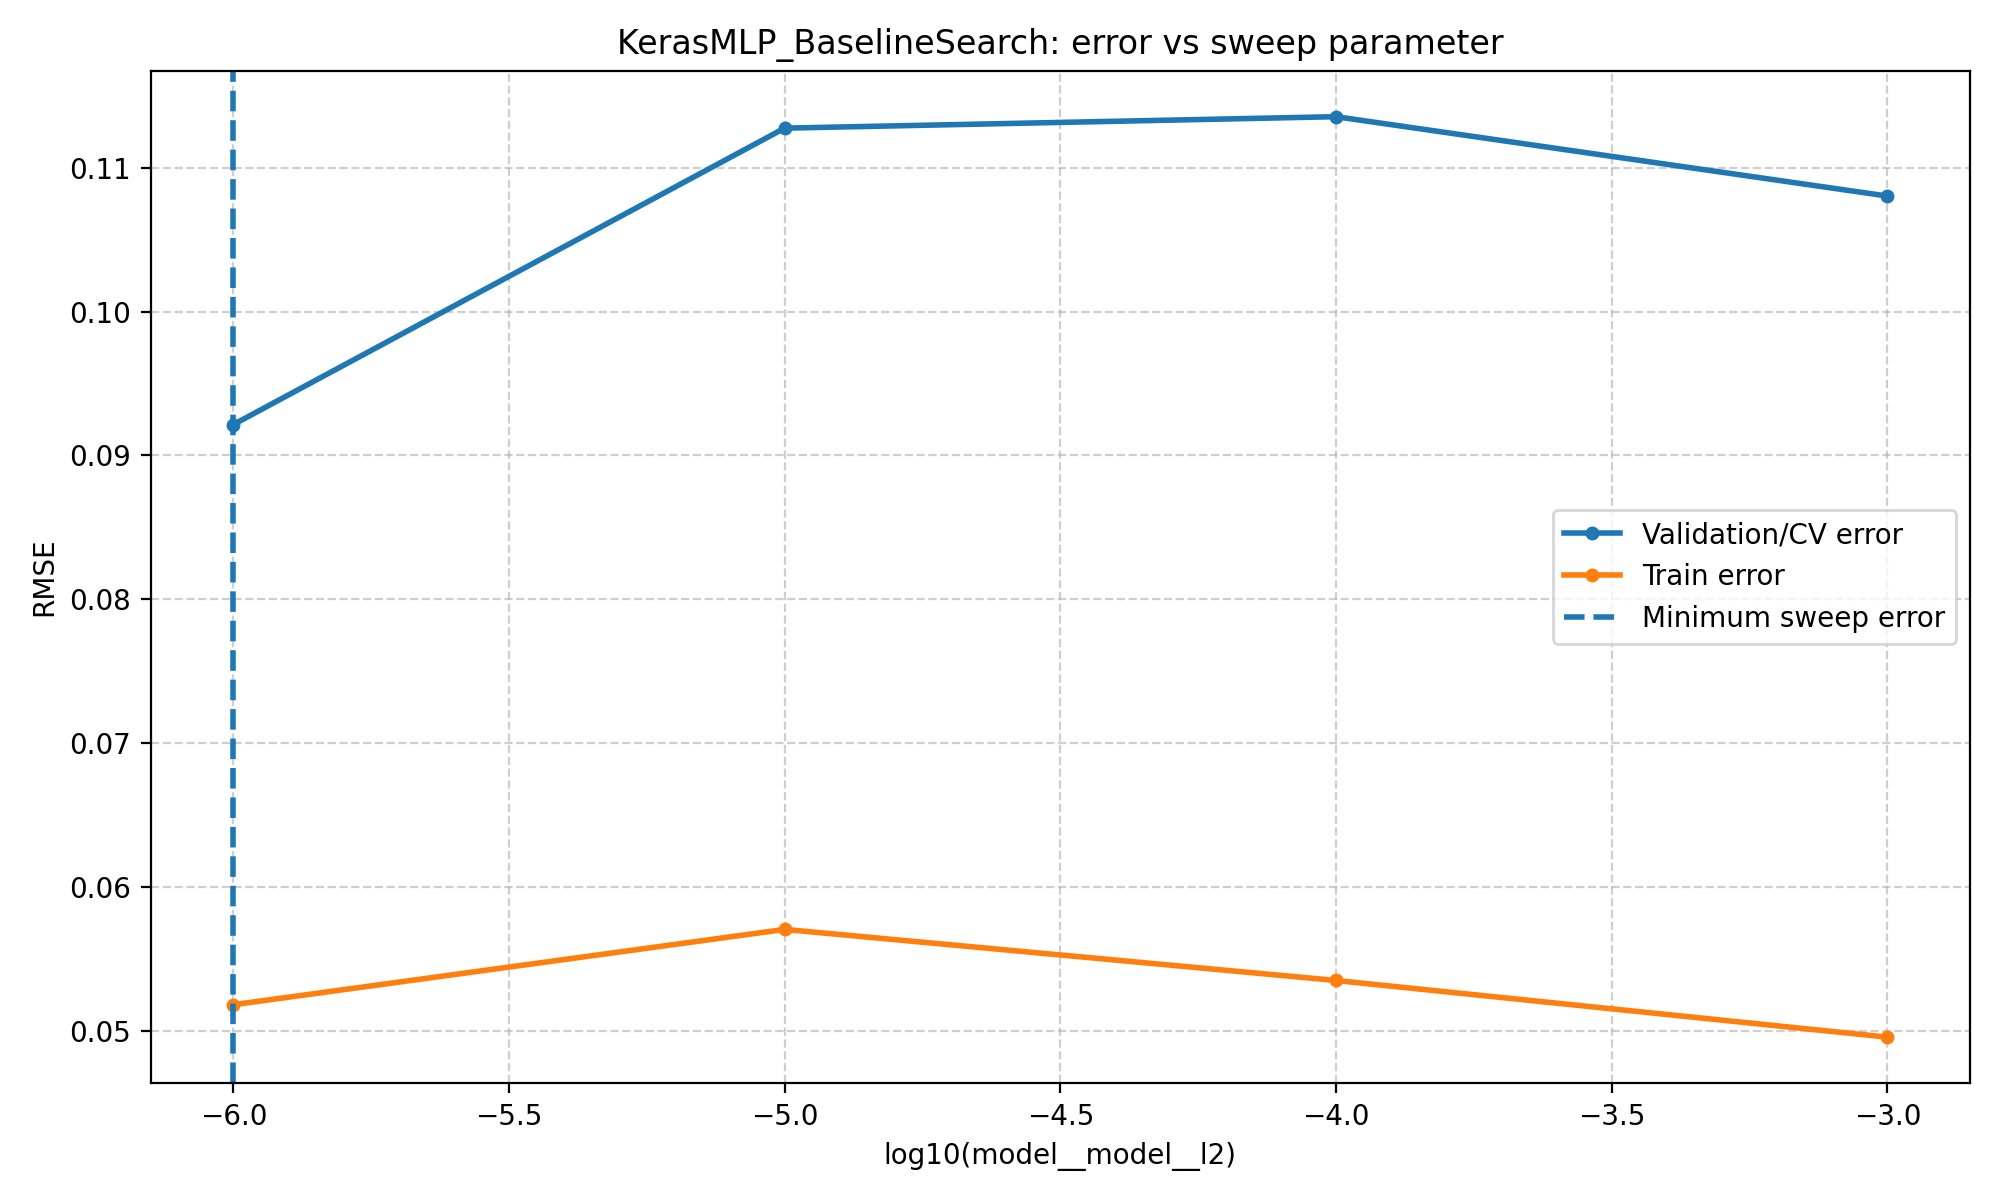
\includegraphics[width=0.82\textwidth]{Imagens/chap06/model_selection/agmd_stage1_baseline_dados_att_com_var_com_phy_error_vs_sweepparam_KerasMLP_BaselineSearch.png}
\caption[Variação do erro com a regularização $L_2$]{Variação do erro de predição em função do hiperparâmetro de regularização $L_2$ durante a etapa de ajuste da rede neural de referência. A linha tracejada indica o menor erro de validação cruzada observado entre os valores testados. A análise permite avaliar a influência da regularização no desempenho do modelo, evidenciando o compromisso entre ajuste aos dados de treinamento e capacidade de generalização. Fonte: Autor.}
\label{fig:error_sweepparam_baseline}
\end{figure}

Na Figura~\ref{fig:error_sweepparam_baseline}, observa-se que o menor erro médio de validação cruzada ocorre na região de $\log_{10}(\lambda_{L2}) = -6$. Esse comportamento indica que, para a rede neural de referência, a introdução de uma penalização $L_2$ de baixa magnitude foi suficiente para melhorar o desempenho em validação em relação às demais configurações avaliadas. Ao mesmo tempo, a presença simultânea dos erros de treinamento e validação permite observar que a escolha do hiperparâmetro não foi feita apenas pelo menor erro de treinamento, mas pelo desempenho estimado em dados não utilizados no ajuste de cada dobra da validação cruzada. Dessa forma, o valor selecionado representa um compromisso entre ajuste aos dados de treinamento e capacidade de generalização.

A arquitetura e os hiperparâmetros selecionados nessa etapa passaram a compor a configuração da rede neural de referência, utilizada como base para as estratégias híbridas avaliadas posteriormente no \textit{pipeline}. A partir dessa configuração inicial, a etapa de ajuste da arquitetura híbrida ZohanResidual manteve a estrutura da rede fixa, variando apenas o hiperparâmetro de regularização $L_2$. Essa escolha permitiu avaliar se, após a incorporação da informação proveniente do modelo físico reduzido, o desempenho do modelo continuava sensível à intensidade da regularização.

A Figura~\ref{fig:error_sweepparam_best_model} apresenta o comportamento do erro de validação cruzada ao longo dessa variação restrita para o modelo híbrido ZohanResidual.

\begin{figure}[H]
\centering

\includegraphics[width=0.82\textwidth]{Imagens/chap06/model_selection/sweep_l2_ZohanResidual.png}
\caption[Variação do erro com a regularização $L_2$ na arquitetura ZohanResidual]{Variação do erro de validação cruzada em função do hiperparâmetro de regularização $L_2$ para a arquitetura híbrida ZohanResidual. Como a estrutura do modelo é mantida fixa, a análise evidencia o efeito da regularização na capacidade de generalização, permitindo identificar a faixa de valores associada ao melhor desempenho preditivo. Fonte: Autor.}
\label{fig:error_sweepparam_best_model}
\end{figure}

Na Figura~\ref{fig:error_sweepparam_best_model}, observa-se que o erro de validação cruzada apresenta pequena variação entre os valores de regularização avaliados. Esse comportamento indica que, na etapa de ajuste restrito, a arquitetura híbrida ZohanResidual não dependeu fortemente de um valor específico de $\lambda_{L2}$ para manter bom desempenho preditivo. Em outras palavras, diferentemente de um cenário em que pequenas alterações no hiperparâmetro provocariam grandes oscilações no erro, o gráfico sugere um comportamento relativamente estável ao longo da faixa analisada.

O valor selecionado corresponde ao menor erro médio de validação cruzada entre as configurações avaliadas. No entanto, a proximidade entre os erros obtidos indica que o ganho associado a essa escolha pontual é limitado. Assim, a principal informação extraída da Figura~\ref{fig:error_sweepparam_best_model} não é apenas o valor ótimo de regularização, mas a baixa sensibilidade da arquitetura híbrida ao hiperparâmetro analisado. Essa estabilidade é relevante no contexto deste trabalho, pois reduz a dependência do desempenho em relação a uma configuração específica e reforça a robustez do modelo dentro da faixa operacional estudada.
\subsection{Comportamento do treinamento da rede neural de referência}

Antes da avaliação da arquitetura híbrida final, foi analisado o comportamento de treinamento da rede neural de referência, utilizada como base para a definição do procedimento de ajuste dos modelos neurais. Essa etapa permitiu verificar a evolução das perdas de treinamento e validação ao longo das épocas, bem como o funcionamento do critério de parada antecipada adotado no treinamento.

A Figura~\ref{fig:learning_curve_baseline} apresenta a evolução das perdas de treinamento e validação ao longo das épocas para a rede neural de referência. O ponto indicado pela linha tracejada corresponde à época selecionada automaticamente pelo mecanismo de \textit{EarlyStopping}.

\begin{figure}[H]
\centering

\includegraphics[width=0.78\textwidth]{Imagens/chap06/model_selection/learning_curve_baseline.png}
\caption[Curvas de treinamento e validação da rede neural de referência]{Curvas de erro para os conjuntos de treinamento e validação ao longo das épocas para a rede neural de referência. A linha tracejada indica a época selecionada pelo critério de parada antecipada (\textit{EarlyStopping}), utilizado para evitar sobreajuste e preservar a capacidade de generalização do modelo. Fonte: Autor.}
\label{fig:learning_curve_baseline}
\end{figure}

Observa-se que tanto a perda de treinamento quanto a perda de validação apresentam redução consistente ao longo das primeiras épocas, indicando aprendizado efetivo do modelo. A partir de aproximadamente 30 épocas, a melhoria na perda de validação torna-se marginal, levando ao acionamento do critério de \textit{EarlyStopping}, que interrompe o treinamento quando não são observadas melhorias adicionais relevantes na validação.

Esse mecanismo é particularmente importante em cenários com conjuntos de dados experimentais limitados, pois evita que a rede continue ajustando seus pesos após o ponto de melhor desempenho em validação. Dessa forma, reduz-se o risco de sobreajuste e aumenta-se a confiabilidade da comparação entre diferentes configurações de modelos neurais.

Com base nesse procedimento, a arquitetura híbrida ZohanResidual foi posteriormente avaliada como modelo final. Diferentemente da rede neural de referência, que aprende diretamente a relação entre as variáveis operacionais e as variáveis de saída, o modelo híbrido incorpora também informação proveniente do modelo físico reduzido. Assim, a rede passa a combinar a flexibilidade da modelagem orientada por dados com uma estimativa fenomenológica prévia do comportamento do sistema.

Dessa forma, a análise da rede de referência não representa o resultado final do trabalho, mas uma etapa necessária para estabelecer o procedimento de treinamento, seleção e controle de sobreajuste utilizado na avaliação das arquiteturas neurais. A partir dessa base, o modelo híbrido ZohanResidual foi selecionado por apresentar melhor desempenho preditivo, mantendo estabilidade de treinamento e boa capacidade de generalização dentro da faixa operacional estudada.
\subsection{Predições fora do conjunto de treinamento na validação cruzada}

A Figura 5.17 apresenta a comparação entre os valores experimentais e as predições obtidas para as amostras mantidas fora do treinamento em cada partição da validação cruzada. Essas predições, denominadas \textit{out-of-fold}, não correspondem a um conjunto de teste externo independente, mas permitem avaliar o desempenho do modelo em observações que não foram utilizadas no ajuste dos parâmetros durante a respectiva rodada de validação.

\begin{figure}[H]
\centering

\begin{subfigure}{0.32\textwidth}
\centering

\includegraphics[width=\textwidth]{Imagens/chap06/model_selection/oof_KerasMLP_ZohanResidual_Restricted_Flux.png}
\caption{$Flux$}
\end{subfigure}
\hfill
\begin{subfigure}{0.32\textwidth}
\centering

\includegraphics[width=\textwidth]{Imagens/chap06/model_selection/oof_KerasMLP_ZohanResidual_Restricted_Alim_T_out.png}
\caption{$Alim\_T_{out}$}
\end{subfigure}
\hfill
\begin{subfigure}{0.32\textwidth}
\centering

\includegraphics[width=\textwidth]{Imagens/chap06/model_selection/oof_KerasMLP_ZohanResidual_Restricted_Ref_T_out.png}
\caption{$Ref\_T_{out}$}
\end{subfigure}

\caption[Predições \textit{out-of-fold} do modelo ZohanResidual]{Predições \textit{out-of-fold} do modelo híbrido ZohanResidual para as três variáveis de saída do sistema. Os gráficos comparam os valores previstos e experimentais para o fluxo de permeado e as temperaturas de saída, considerando as amostras mantidas fora do treinamento em cada partição da validação cruzada. Fonte: Autor.}
\label{fig:best_model_oof_predictions}
\end{figure}

Observa-se concordância entre os valores experimentais e os valores previstos, especialmente para o alvo $Flux$, que foi priorizado no processo de seleção. A proximidade de grande parte dos pontos em relação à reta identidade indica que o modelo foi capaz de representar as principais tendências presentes nos dados experimentais. Ao mesmo tempo, as dispersões observadas em determinadas regiões do espaço de operação indicam que ainda existem desvios residuais, sobretudo em condições nas quais a variabilidade experimental ou a menor densidade de amostras pode dificultar a predição.

Em conjunto, os resultados apresentados ao longo desta análise indicam que a arquitetura híbrida selecionada combina bom desempenho preditivo com estabilidade de treinamento e baixa sensibilidade aos hiperparâmetros avaliados. Essas características são desejáveis em aplicações com conjuntos de dados experimentais, onde o risco de sobreajuste e a dependência do desempenho em relação à partição dos dados e às configurações escolhidas são fatores relevantes. Nesse sentido, a menor sensibilidade observada sugere maior robustez do modelo dentro da faixa operacional estudada.
\section{Comparação entre o modelo físico reduzido e o modelo final híbrido}
\label{subsec:comparacao_modelo_fisico_modelo_final}

Por fim, realizou-se a comparação entre o modelo físico reduzido utilizado como referência fenomenológica e o modelo final híbrido selecionado neste trabalho. Essa análise é central para a interpretação dos resultados, pois permite avaliar se a incorporação de técnicas de aprendizado de máquina, combinadas à informação física previamente disponível, trouxe ganhos efetivos em relação ao modelo físico 0D isolado.

O modelo físico reduzido representa uma descrição simplificada do processo V-AGMD, construída a partir de hipóteses fenomenológicas e relações de transferência de calor e massa. Embora esse tipo de abordagem seja fundamental para compreender o comportamento do sistema, sua capacidade preditiva pode ser limitada pelas simplificações adotadas e pela dificuldade de representar integralmente os efeitos acoplados presentes no processo. Nesse contexto, o modelo híbrido ZohanResidual foi avaliado como uma alternativa capaz de preservar a informação física fornecida pelo modelo 0D, ao mesmo tempo em que aprende, a partir dos dados experimentais, correções associadas ao comportamento real do sistema.

\begin{table}[H]
\centering
\caption{Comparação entre o modelo físico reduzido e o modelo híbrido final.}
\begin{tabular}{lccc}
\toprule
Modelo & RMSE$_{Alim}$ & RMSE$_{Ref}$ & RMSE$_{Flux}$ \\
\midrule
Modelo físico 0D & 1.613 & 0.927 & 0.215 \\
Modelo híbrido ZohanResidual & 0.290 & 0.385 & \textbf{0.061} \\
\bottomrule
\end{tabular}
\end{table}

\begin{figure}[H]
    \centering
    
    \begin{subfigure}[b]{0.48\linewidth}
        \centering
        
\includegraphics[width=\linewidth]{Imagens/chap06/overlay_ZohanResidual_Flux.png}
        \caption{Fluxo de permeado}
    \end{subfigure}
    \hfill
    \begin{subfigure}[b]{0.48\linewidth}
        \centering
        
\includegraphics[width=\linewidth]{Imagens/chap06/overlay_ZohanResidual_Ref_T_out.png}
        \caption{Temperatura de saída do circuito de resfriamento}
    \end{subfigure}

    \vspace{0.5cm}

    \begin{subfigure}[b]{0.48\linewidth}
        \centering
        
\includegraphics[width=\linewidth]{Imagens/chap06/overlay_ZohanResidual_Alim_T_out.png}
        \caption{Temperatura de saída da alimentação}
    \end{subfigure}

    \caption[Comparação entre valores experimentais e predições dos modelos físico e híbrido]{Comparação entre os valores experimentais e as predições do modelo físico 0D e do modelo híbrido ZohanResidual para as variáveis de saída do sistema. Os gráficos permitem avaliar a capacidade de cada abordagem em reproduzir o comportamento do fluxo de permeado e das temperaturas de saída ao longo dos dados experimentais, evidenciando o ganho preditivo obtido com a incorporação de informação orientada por dados. Fonte: Autor.}
    \label{fig:overlay_hibrido}
\end{figure}

Os resultados indicam que o modelo híbrido ZohanResidual apresentou redução expressiva do erro em relação ao modelo físico reduzido para as três variáveis analisadas. Para o fluxo de permeado, variável priorizada na seleção dos modelos, o RMSE foi reduzido de 0,215 para 0,061. Também foram observados ganhos nas temperaturas de saída, com redução do erro de 1,613 para 0,290 em $Alim\_T\_out$ e de 0,927 para 0,385 em $Ref\_T\_out$.

Esse resultado mostra que o modelo físico 0D, embora seja capaz de representar tendências gerais do sistema, não captura integralmente as relações presentes nos dados experimentais. A arquitetura híbrida, por sua vez, foi capaz de utilizar a informação física como referência inicial e aprender ajustes orientados pelos dados, reduzindo os desvios em relação às medições experimentais. Assim, o ganho obtido não decorre apenas do uso de uma rede neural mais flexível, mas da combinação entre uma representação fenomenológica do processo e uma etapa de correção empírica baseada nos dados disponíveis.

Dessa forma, a principal contribuição deste trabalho está em demonstrar que, para o sistema V-AGMD analisado, a abordagem híbrida apresentou vantagem em relação ao uso isolado do modelo físico reduzido. Esse resultado é particularmente relevante porque sistemas de destilação por membranas envolvem fenômenos acoplados de transferência de calor e massa, cuja modelagem puramente fenomenológica pode exigir hipóteses simplificadoras. A incorporação de aprendizado orientado por dados permite complementar essa descrição física, melhorando a capacidade preditiva dentro da faixa operacional estudada.

Portanto, a comparação entre o modelo físico 0D e o modelo híbrido ZohanResidual evidencia o valor da estratégia adotada ao longo deste trabalho: partir de uma base física conhecida, avaliar diferentes famílias de modelos e verificar se a informação experimental disponível poderia ser utilizada para melhorar a predição das variáveis de desempenho. Os resultados obtidos indicam que essa estratégia foi bem-sucedida, reforçando o potencial de abordagens híbridas físico-orientadas por dados como ferramenta de modelagem para sistemas V-AGMD.
    \chapter{Conclusões}
\label{chap:conclusoes}

Este trabalho teve como objetivo investigar a aplicação de técnicas de modelagem baseada em dados e de modelagem híbrida, com incorporação de informação física, para a predição de variáveis de desempenho em sistemas de destilação por membranas do tipo V-AGMD. O estudo concentrou-se na previsão do fluxo de permeado e das temperaturas de saída das correntes de alimentação e resfriamento a partir de variáveis operacionais do sistema, por meio de um \textit{pipeline} que integrou análise exploratória dos dados, validação cruzada com separação por regimes experimentais, comparação entre diferentes famílias de modelos e uso de predições oriundas de um modelo físico reduzido do processo.

\subsection{Conclusões gerais e interpretação dos resultados}

A partir das métricas observadas, verificou-se que o melhor desempenho foi obtido pelo modelo híbrido HRNN, isto é, uma rede neural multicamada com incorporação das predições do modelo físico 0D e de restrições baseadas no comportamento fenomenológico do sistema. Esse modelo apresentou redução do erro quadrático médio da raiz (RMSE) em relação ao melhor modelo linear e ao melhor modelo baseado em árvores.

A performance competitiva das famílias de modelos lineares sugere que, na faixa operacional analisada, uma parcela relevante da variabilidade dos alvos pode ser representada por relações de menor complexidade. Ainda assim, o ganho obtido pelo modelo híbrido indica que a representação não linear da rede neural, combinada à informação física fornecida pelo modelo 0D, permitiu capturar efeitos adicionais associados ao acoplamento entre transferência de calor e massa no processo.

Do ponto de vista conceitual, esse resultado pode ser interpretado como uma aproximação de um cenário ideal de modelagem híbrida. O modelo mais adequado para representar o comportamento do sistema seria aquele capaz de reproduzir, de forma eficiente, as equações de balanço de massa e energia e, simultaneamente, incorporar as imperfeições observadas na operação real. Nesse sentido, a estratégia adotada se aproxima desse objetivo ao combinar as predições do modelo físico reduzido com uma rede neural treinada para aprender correções sistemáticas em relação aos dados experimentais.

Sob essa perspectiva, a rede neural fornece uma estrutura capaz de aproximar relações não lineares complexas, enquanto o modelo físico 0D representa, de forma simplificada ou média, os principais acoplamentos fenomenológicos do sistema. A combinação dessas duas abordagens permite que o modelo híbrido incorpore tanto a informação empírica presente nos dados quanto uma tendência física previamente estimada pelo modelo fenomenológico. No entanto, essa aproximação permanece limitada à região de operação contemplada pelos dados experimentais. Assim, mesmo com a incorporação de informação física, a capacidade de generalização do modelo continua dependente da cobertura dos dados disponíveis e não deve ser interpretada como garantia de extrapolação para condições operacionais não avaliadas experimentalmente.

Essa interpretação é particularmente relevante porque o modelo físico reduzido está sujeito a simplificações inerentes à sua formulação. Assim, a rede híbrida atua como um corretor sistemático das discrepâncias entre o modelo físico e o comportamento experimental. Essa complementaridade mostrou-se mais eficaz do que o uso isolado de modelos puramente \textit{data-driven} ou puramente \textit{physics-driven}, ao menos dentro da faixa de operação investigada.

A análise também deve considerar os fundamentos estatísticos da capacidade de generalização. Modelos mais flexíveis podem apresentar excelente ajuste ao conjunto de treinamento sem necessariamente reproduzir novos dados com precisão, especialmente na presença de ruído experimental. Nesse trabalho, o uso de validação cruzada e critérios de seleção com penalização de complexidade foi fundamental para reduzir o risco de sobreajuste. O bom desempenho do modelo HRNN sugere que sua maior flexibilidade foi adequadamente regularizada, permitindo capturar relações consistentes nos dados.


Além disso, as diferentes variáveis de saída estão fisicamente acopladas. O fluxo de permeado depende diretamente dos gradientes térmicos e de pressão de vapor estabelecidos no módulo, bem como das resistências térmicas e difusivas e dos efeitos de polarização. Ao mesmo tempo, as temperaturas de saída também são afetadas pela transferência de massa, uma vez que a evaporação e a condensação do permeado envolvem trocas de calor latente e alteram os balanços de energia nas correntes de alimentação e refrigeração. Assim, embora a seleção de modelos tenha sido orientada prioritariamente pelo erro associado ao fluxo de permeado, a previsão das temperaturas permanece como uma avaliação relevante da capacidade do modelo em representar o comportamento térmico acoplado do sistema.

Os resultados obtidos indicam que, mesmo sem terem sido priorizadas explicitamente no critério de seleção, as temperaturas de saída apresentaram desempenho preditivo elevado. Isso sugere que a arquitetura selecionada foi capaz de capturar, de forma satisfatória, não apenas a variável principal de produtividade, mas também as respostas térmicas associadas ao funcionamento do processo.


Por fim, destaca-se que a estratégia de seleção de modelos foi deliberadamente orientada pela previsão do fluxo de permeado, por este representar o principal indicador de produtividade do processo. Embora todos os modelos tenham sido treinados para prever simultaneamente o fluxo e as temperaturas de saída, a busca e a seleção de hiperparâmetros utilizaram como critério principal o erro associado ao alvo $Flux$. Assim, o mesmo procedimento de priorização não foi repetido separadamente para $Alim\_T\_out$ e $Ref\_T\_out$, a fim de manter uma única estratégia de seleção alinhada ao objetivo central do trabalho e evitar a escolha de modelos distintos para cada variável de saída.

Ainda assim, as temperaturas de saída foram mantidas na avaliação por sua relevância física e energética, uma vez que influenciam diretamente métricas como o consumo específico de energia térmica ($SEC$) e a razão de ganho de saída ($GOR$). Além disso, mesmo não tendo sido priorizadas no critério de seleção, essas variáveis apresentaram desempenho preditivo elevado, indicando que a estratégia adotada foi capaz de preservar uma boa representação das respostas térmicas do sistema. Dessa forma, os resultados obtidos para essas variáveis devem ser interpretados como uma avaliação complementar do modelo selecionado com base no fluxo de permeado.

\subsection{Trabalhos futuros}

A partir dos resultados obtidos, diversas possibilidades de aprofundamento podem ser propostas.

Uma primeira direção consiste em investigar estratégias de modelagem que priorizem explicitamente a predição das temperaturas de saída, por meio de critérios de seleção orientados por erro térmico ou buscas de hiperparâmetros dedicadas a essas variáveis.

Outra linha promissora envolve o refinamento das estratégias de incorporação de conhecimento físico. Embora a abordagem híbrida adotada tenha apresentado bons resultados, ainda é possível explorar outras formas de regularização física, incluindo funções de perda híbridas ou arquiteturas que imponham maior consistência com balanços de energia e massa.

Também pode ser interessante avaliar o uso de \textit{Physics-Informed Neural Networks} (PINNs), especialmente em cenários onde se deseja ampliar a capacidade de generalização para regiões operacionais pouco amostradas. No entanto, para a faixa considerada neste estudo, as estratégias híbridas já se mostraram adequadas.

Uma ampliação natural deste trabalho consiste na obtenção de novos dados experimentais em regiões mais amplas do espaço de operação. Isso permitiria avaliar a robustez dos modelos fora da região atualmente analisada e explorar de forma mais clara possíveis não linearidades do sistema.

Por fim, os modelos desenvolvidos podem ser aplicados em estudos de otimização operacional, permitindo identificar condições de operação que maximizem a produtividade, minimizem o consumo energético ou conciliem ambos os objetivos.

Em síntese, este trabalho mostrou que a integração entre modelos físicos reduzidos e aprendizado de máquina constitui uma abordagem eficaz para a modelagem de sistemas V-AGMD. Os resultados reforçam que a combinação entre conhecimento fenomenológico, validação estatística rigorosa e estratégias de modelagem híbrida é fundamental para obter modelos preditivos robustos, interpretáveis e relevantes do ponto de vista de engenharia.

  \backmatter
  %\nocite{*}
  \bibliographystyle{coppe-unsrt}
  \bibliography{thesis}
  \appendix
  \chapter{Resultados Análises Descartadas de Pré-processamento}
\label{apendice}

\begin{table}[H]
\centering
\caption{Avaliação do impacto da geração de dados sintéticos no desempenho preditivo dos modelos. Foram comparados modelos treinados apenas com dados experimentais reais e modelos treinados com a combinação de dados reais e dados sintéticos gerados a partir do conjunto de treinamento. As métricas apresentadas correspondem ao erro no conjunto de teste composto exclusivamente por dados reais.}
\label{tab:avaliacao_data_augmentation}
\small
\setlength{\tabcolsep}{6pt}
\begin{tabular}{llcccc}
\toprule
\textbf{Alvo} & \textbf{Modelo} & \textbf{Treino} & \textbf{RMSE} & \textbf{MAE} & $\boldsymbol{R^2}$ \\
\midrule

\multirow{6}{*}{\textit{Flux}}
 & Regressão Linear & Real & 0.077 & 0.057 & 0.965 \\
 & Regressão Linear & Real + Sintético & 0.077 & 0.061 & 0.965 \\
 & Random Forest & Real & 0.103 & 0.084 & 0.937 \\
 & Random Forest & Real + Sintético & 0.081 & 0.068 & 0.961 \\
 & MLP (tf.keras) & Real & 0.053 & 0.037 & 0.983 \\
 & MLP (tf.keras) & Real + Sintético & 0.077 & 0.056 & 0.965 \\
\midrule

\multirow{6}{*}{\textit{Alim\_T\_out}}
 & Regressão Linear & Real & 0.165 & 0.128 & 0.973 \\
 & Regressão Linear & Real + Sintético & 0.239 & 0.175 & 0.943 \\
 & Random Forest & Real & 0.386 & 0.287 & 0.851 \\
 & Random Forest & Real + Sintético & 0.266 & 0.210 & 0.930 \\
 & MLP (tf.keras) & Real & 0.106 & 0.087 & 0.989 \\
 & MLP (tf.keras) & Real + Sintético & 0.287 & 0.211 & 0.918 \\
\midrule

\multirow{6}{*}{\textit{Ref\_T\_out}}
 & Regressão Linear & Real & 0.170 & 0.119 & 0.998 \\
 & Regressão Linear & Real + Sintético & 0.246 & 0.178 & 0.996 \\
 & Random Forest & Real & 0.665 & 0.486 & 0.968 \\
 & Random Forest & Real + Sintético & 0.412 & 0.302 & 0.988 \\
 & MLP (tf.keras) & Real & 0.176 & 0.121 & 0.998 \\
 & MLP (tf.keras) & Real + Sintético & 0.262 & 0.204 & 0.995 \\
\bottomrule
\end{tabular}
\end{table}


\begin{table}[H]
\centering
\small
\setlength{\tabcolsep}{5pt}
\caption{Melhores configurações de discretização (\textit{binning}) obtidas no estudo exploratório realizado com regressão linear. Para cada variável de saída são apresentadas as cinco configurações com melhor desempenho entre as 32 combinações possíveis de discretização das variáveis de entrada. O caso \textit{baseline} corresponde ao modelo treinado com todas as variáveis contínuas. As métricas correspondem ao desempenho médio obtido por validação cruzada com \textit{GroupKFold}.}
\label{tab:binning_resultados_apendice}
\begin{tabular}{lcccccc}
\toprule
\textbf{Alvo} & \textbf{Rank} & \textbf{Config ID} & \textbf{Variáveis discretizadas} & \textbf{$n_{bin}$} & \textbf{RMSE} & \textbf{$R^2$} \\
\midrule

\multirow{5}{*}{Flux}
 & 1 & 0  & none (baseline) & 0 & 0.0821 & 0.9140 \\
 & 2 & 16 & Ref\_T\_in & 1 & 0.0822 & 0.9140 \\
 & 3 & 2  & P\_vacuum & 1 & 0.1017 & 0.8460 \\
 & 4 & 18 & Ref\_T\_in,P\_vacuum & 2 & 0.1029 & 0.8400 \\
 & 5 & 8  & Alim\_T\_in & 1 & 0.1199 & 0.8150 \\

\midrule

\multirow{5}{*}{Alim\_T\_out}
 & 1 & 8  & Alim\_T\_in & 1 & 0.452 & 0.966 \\
 & 2 & 0  & none (baseline) & 0 & 0.514 & 0.955 \\
 & 3 & 26 & Alim\_T\_in,Ref\_V\_in,P\_vacuum & 3 & 0.676 & 0.932 \\
 & 4 & 10 & Alim\_T\_in,P\_vacuum & 2 & 0.823 & 0.903 \\
 & 5 & 6  & Ref\_V\_in,P\_vacuum & 2 & 0.760 & 0.920 \\

\midrule

\multirow{5}{*}{Ref\_T\_out}
 & 1 & 5  & Ref\_V\_in,C\_NaCl & 2 & 0.142 & 0.996 \\
 & 2 & 21 & Ref\_T\_in,Ref\_V\_in,C\_NaCl & 3 & 0.147 & 0.996 \\
 & 3 & 0  & none (baseline) & 0 & 0.148 & 0.996 \\
 & 4 & 16 & Ref\_T\_in & 1 & 0.146 & 0.996 \\
 & 5 & 29 & Ref\_T\_in,Ref\_V\_in,P\_vacuum,C\_NaCl & 4 & 0.191 & 0.994 \\

\bottomrule
\end{tabular}
\end{table}

\begin{table}[H]
\centering
\caption{Resultados da análise de seleção de preditores utilizando \textit{Best Subset Selection}. São apresentados os melhores subconjuntos para $k = 3, 4, 5$ variáveis de entrada, juntamente com as métricas de desempenho RMSE e $R^2$ para cada variável de saída.}
\label{sec:apendice_binning}

% diminui um pouco o espaço horizontal entre colunas
\setlength{\tabcolsep}{4pt}

\begin{tabular}{c p{3.5cm} cccc ccc}
\toprule
$k$ 
& Subconjunto 
& RMSE$_{\mathrm{Flux}}$
& RMSE$_{\mathrm{Alim\_T\_out}}$
& RMSE$_{\mathrm{Ref\_T\_out}}$
& $R^2_{\mathrm{Flux}}$
& $R^2_{\mathrm{Alim}}$
& $R^2_{\mathrm{Ref}}$ \\
\midrule

3 &
\shortstack[l]{Ref\_T\_in\\Alim\_T\_in\\C\_NaCl}
& 0.222 & 0.625 & 0.604
& 0.744 & 0.817 & 0.810 \\

4 &
\shortstack[l]{Ref\_T\_in\\Alim\_T\_in\\V\_in\\C\_NaCl}
& 0.142 & 0.389 & 0.398
& 0.887 & 0.909 & 0.900 \\

5 &
\shortstack[l]{Ref\_T\_in\\Alim\_T\_in\\V\_in\\P\_vacuum\\C\_NaCl}
& \textbf{0.082} & \textbf{0.227} & \textbf{0.242}
& \textbf{0.953} & \textbf{0.960} & \textbf{0.952} \\

\bottomrule
\end{tabular}

% se quiser, pode voltar o tabcolsep ao valor padrão depois:
% \setlength{\tabcolsep}{6pt}

\end{table}

% Tabela gerada a partir de dados_att_com_var_com_phy.csv
% Colunas mantidas: variáveis de entrada e saídas experimentais principais.
% Pacotes necessários no preâmbulo: \usepackage{longtable} e \usepackage{booktabs}.

\begingroup
\small
\setlength{\tabcolsep}{2.5pt}
\renewcommand{\arraystretch}{1.08}
\begin{longtable}{@{}cccccccc@{}}
\caption[Dados experimentais utilizados na modelagem]{Dados experimentais utilizados na modelagem, contendo as variáveis de entrada e as variáveis de saída consideradas. Fonte: Autor.}
\label{tab:dados_modelagem}\\
\toprule
\textbf{Ref\_T\_in} & \textbf{Alim\_T\_in} & \textbf{Ref\_V\_in} & \textbf{P\_vacuum} & \textbf{C\_NaCl} & \textbf{Alim\_T\_out} & \textbf{Ref\_T\_out} & \textbf{Flux} \\
\midrule
\endfirsthead

\caption[]{Dados experimentais utilizados na modelagem -- continuação.}\\
\toprule
\textbf{Ref\_T\_in} & \textbf{Alim\_T\_in} & \textbf{Ref\_V\_in} & \textbf{P\_vacuum} & \textbf{C\_NaCl} & \textbf{Alim\_T\_out} & \textbf{Ref\_T\_out} & \textbf{Flux} \\
\midrule
\endhead

\midrule
\multicolumn{8}{r}{Continua na próxima página}\\
\endfoot

\bottomrule
\endlastfoot

30,0039 & 59,9941 & 600,0674 & -495,9198 & 10,1766 & 33,4887 & 55,8363 & 1,4075 \\
29,8254 & 60,0219 & 599,9456 & -497,0388 & 10,1044 & 33,4237 & 56,0092 & 1,4288 \\
30,1556 & 60,031 & 599,9733 & -495,7314 & 10,0902 & 33,6627 & 56,0744 & 1,4075 \\
29,7888 & 70,0173 & 600,0697 & -494,3425 & 10,6082 & 34,0641 & 64,7119 & 2,0988 \\
29,9799 & 69,9936 & 599,9224 & -494,92 & 10,0578 & 34,2121 & 64,7208 & 2,0487 \\
30,1331 & 70,0333 & 599,9431 & -495,232 & 9,7985 & 34,3609 & 64,8056 & 2,0052 \\
30,1662 & 70,0642 & 400,0134 & -496,0848 & 10,0918 & 33,3564 & 66,112 & 1,3868 \\
29,8357 & 69,9958 & 399,9848 & -495,8688 & 9,9627 & 33,1354 & 66,0814 & 1,3668 \\
30,1315 & 70,04 & 399,9935 & -496,6191 & 9,9805 & 33,3162 & 66,0898 & 1,3848 \\
30,1515 & 70,0067 & 600,0763 & -498,6704 & 10,1131 & 34,339 & 64,7182 & 2,0052 \\
30,0491 & 70,0203 & 600,0193 & -498,0134 & 10,3245 & 34,4295 & 64,7837 & 2,0052 \\
29,9598 & 69,9925 & 600,0828 & -497,9761 & 10,5268 & 34,3078 & 64,7561 & 2,0487 \\
30,027 & 59,9964 & 599,9482 & -13,2443 & 10,0265 & 34,3692 & 55,0317 & 1,0843 \\
30,0169 & 60,0132 & 600,0082 & -13,193 & 10,2317 & 34,3832 & 55,018 & 1,123 \\
29,9076 & 60,0254 & 600,0753 & -13,2736 & 10,3689 & 34,3098 & 55,0008 & 1,123 \\
30,0707 & 60,0179 & 399,856 & -13,1944 & 10,0115 & 33,3257 & 55,9979 & 0,857 \\
29,9735 & 60,0185 & 399,963 & -13,164 & 10,0258 & 33,2663 & 55,9708 & 0,8729 \\
29,965 & 59,9829 & 399,8922 & -13,2655 & 10,1225 & 33,2044 & 55,9284 & 0,8818 \\
29,9661 & 70,0255 & 399,9647 & -13,5431 & 9,9731 & 34,0834 & 64,7498 & 1,1351 \\
30,08 & 69,9831 & 399,9042 & -13,3784 & 10,1673 & 34,1634 & 64,729 & 1,123 \\
29,8542 & 70,0012 & 399,9354 & -13,3309 & 10,3119 & 34,0391 & 64,6666 & 1,1098 \\
30,0212 & 70,0109 & 600,0116 & -13,4019 & 10,174 & 35,7794 & 63,3489 & 1,598 \\
29,8547 & 69,976 & 600,0544 & -13,5735 & 10,0424 & 35,5309 & 63,2641 & 1,6255 \\
30,1531 & 69,9445 & 599,9392 & -13,643 & 10,2275 & 35,8346 & 63,2954 & 1,598 \\
27,6592 & 70,001 & 600,2088 & -495,5513 & 9,9584 & 32,1167 & 64,4304 & 2,0988 \\
27,5992 & 69,9847 & 600,0342 & -497,6389 & 10,0293 & 32,0682 & 64,4082 & 2,0487 \\
27,5091 & 69,9998 & 600,0746 & -497,3625 & 10,1367 & 31,9924 & 64,4112 & 2,0941 \\
27,4488 & 69,978 & 400,049 & -497,3706 & 9,8546 & 30,7496 & 65,6165 & 1,4288 \\
27,528 & 70,0246 & 400,049 & -497,1626 & 9,9882 & 30,7895 & 65,6175 & 1,4288 \\
27,6043 & 69,9994 & 400,0353 & -497,8379 & 10,1277 & 30,8799 & 65,6201 & 1,4288 \\
27,6635 & 69,9925 & 599,9754 & -497,4785 & 9,7619 & 32,2274 & 64,3159 & 2,0988 \\
27,4945 & 70,0239 & 600,0499 & -495,1225 & 9,7325 & 32,1619 & 64,3405 & 2,0941 \\
27,5376 & 69,9668 & 600,1143 & -496,4073 & 9,7899 & 32,1302 & 64,2812 & 2,0941 \\
27,5156 & 60,0192 & 600,018 & -496,5466 & 10,0437 & 31,3444 & 55,5079 & 1,4967 \\
27,4617 & 59,9896 & 599,9932 & -498,5424 & 10,0722 & 31,2881 & 55,4588 & 1,4734 \\
27,5202 & 59,9742 & 599,9752 & -496,5228 & 10,1867 & 31,3257 & 55,5026 & 1,4967 \\
27,6115 & 60 & 399,9878 & -499,982 & 9,9116 & 30,4335 & 56,405 & 1,0255 \\
27,4585 & 59,9993 & 400,0594 & -498,4182 & 9,9642 & 30,3533 & 56,402 & 1,0026 \\
27,4463 & 59,9924 & 399,9546 & -497,9494 & 10,0211 & 30,2822 & 56,4023 & 1,0367 \\
27,4595 & 70,0122 & 399,9688 & -12,6355 & 9,7971 & 31,8771 & 64,8127 & 1,149 \\
27,528 & 70,0386 & 400,0735 & -12,4415 & 9,9795 & 31,9615 & 64,8452 & 1,1365 \\
27,5277 & 70,0135 & 400,0763 & -12,3846 & 10,001 & 31,9249 & 64,835 & 1,1645 \\
27,4911 & 69,9973 & 600,0356 & -12,5653 & 10,0673 & 33,4242 & 63,416 & 1,654 \\
27,4507 & 70,0142 & 600,2162 & -12,593 & 10,0365 & 33,361 & 63,4483 & 1,7457 \\
27,4818 & 69,9998 & 599,9884 & -12,6691 & 9,9599 & 33,3519 & 63,4357 & 1,6569 \\
27,4208 & 60,0023 & 599,9947 & -12,4171 & 9,9554 & 32,2507 & 54,8449 & 1,149 \\
27,5558 & 60,0097 & 600,0351 & -12,4654 & 10,0492 & 32,38 & 54,8331 & 1,1217 \\
27,565 & 59,9807 & 600,1117 & -12,5032 & 9,957 & 32,4041 & 54,7915 & 1,1365 \\
27,4636 & 59,9878 & 399,9365 & -12,0643 & 9,989 & 31,0132 & 55,7266 & 0,7864 \\
27,5387 & 60,025 & 400,0876 & -12,126 & 10,1038 & 31,0449 & 55,745 & 0,7851 \\
27,4987 & 59,9888 & 400,0837 & -12,192 & 10,2291 & 31,0581 & 55,7275 & 0,7735 \\
27,4238 & 70,0221 & 400,3442 & -12,6156 & 10,0519 & 31,7147 & 64,6189 & 1,1776 \\
27,4519 & 69,9729 & 399,9702 & -12,5775 & 10,1537 & 31,7206 & 64,6026 & 1,1365 \\
27,5644 & 69,9755 & 399,9865 & -12,5041 & 10,2489 & 31,8531 & 64,642 & 1,1351 \\
27,513 & 59,9972 & 600,1341 & -12,4884 & 9,1672 & 32,2986 & 54,6964 & 1,2746 \\
27,5037 & 60,0009 & 599,9152 & -12,4582 & 9,1176 & 32,2969 & 54,6355 & 1,225 \\
27,4847 & 59,9962 & 600,0447 & -12,5091 & 9,1334 & 32,2969 & 54,6153 & 1,1631 \\
28,7879 & 65,0088 & 499,9809 & -243,796 & 10,5464 & 32,6495 & 60,2257 & 1,3265 \\
28,7936 & 65,019 & 499,9999 & -249,7162 & 10,6651 & 32,6378 & 60,2909 & 1,2746 \\
28,7673 & 64,9928 & 499,977 & -249,1824 & 10,6452 & 32,5881 & 60,3142 & 1,3099 \\
30,0619 & 60,0097 & 400,1677 & -498,062 & 10,7152 & 32,6478 & 56,6433 & 0,9072 \\
29,9926 & 60,0001 & 400,1172 & -497,6219 & 10,8231 & 32,5728 & 56,6653 & 0,8978 \\
29,8468 & 60,0157 & 399,9632 & -497,4666 & 11,0157 & 32,4079 & 56,6076 & 1,0482 \\
29,9171 & 65,016 & 599,9569 & -496,9667 & 9,8817 & 33,821 & 60,2526 & 1,654 \\
29,8634 & 65,0043 & 599,9766 & -497,1768 & 9,9843 & 33,7657 & 60,2597 & 1,654 \\
30,0075 & 64,9606 & 600,0592 & -497,1557 & 10,0294 & 33,8489 & 60,2461 & 1,654 \\
29,8972 & 64,9975 & 399,9771 & -500,0974 & 10,4899 & 32,743 & 61,2205 & 1,1504 \\
30,1827 & 65,0037 & 400,0735 & -500,0799 & 10,314 & 32,9853 & 61,2283 & 1,1365 \\
29,9987 & 65,0051 & 400,0117 & -499,1587 & 10,465 & 32,874 & 61,2422 & 1,123 \\
28,0401 & 66,9949 & 549,9297 & -401,8945 & 10,8434 & 32,1568 & 61,9238 & 1,6835 \\
27,8744 & 66,9918 & 549,9136 & -399,0726 & 10,726 & 32,0083 & 61,8653 & 1,6835 \\
27,8335 & 67,0146 & 550,0059 & -393,9004 & 10,5701 & 31,9878 & 61,8571 & 1,6865 \\
30,0827 & 70,0211 & 600,1758 & -497,5336 & 66,4137 & 35,0677 & 64,2703 & 1,4734 \\
29,8684 & 70,0299 & 600,059 & -499,1438 & 68,4599 & 34,8792 & 64,2502 & 1,4508 \\
29,9293 & 70,0285 & 599,9934 & -497,7891 & 70,7963 & 34,9075 & 64,2326 & 1,4288 \\
30,1173 & 59,9945 & 599,976 & -500,8093 & 67,1271 & 34,1742 & 55,4281 & 0,916 \\
30,0132 & 60,0148 & 599,9672 & -500,4416 & 65,6128 & 34,0578 & 55,4348 & 0,9152 \\
29,9512 & 59,9951 & 599,965 & -497,9369 & 66,6335 & 34,0134 & 55,406 & 0,9152 \\
29,9838 & 69,9964 & 400,0021 & -499,0079 & 71,8814 & 33,9291 & 65,1912 & 0,8343 \\
30,0059 & 70,0079 & 400,0028 & -499,0821 & 75,0587 & 33,9478 & 65,196 & 0,827 \\
29,9499 & 70,0052 & 399,9709 & -499,1066 & 77,2158 & 33,9711 & 65,2201 & 0,827 \\
30,029 & 60,0061 & 399,9841 & -500,0113 & 63,4706 & 33,2443 & 56,2766 & 0,5391 \\
30,034 & 59,9932 & 399,9708 & -499,9284 & 64,8846 & 33,228 & 56,2494 & 0,5209 \\
29,9545 & 59,9982 & 399,9773 & -500,3441 & 67,485 & 33,2018 & 56,2442 & 0,5069 \\
31,939 & 70,0031 & 600,0263 & -12,3929 & 75,6606 & 37,5831 & 63,5963 & 0,9931 \\
31,8518 & 69,9803 & 600,026 & -12,3641 & 73,972 & 37,5394 & 63,6099 & 0,9818 \\
31,6705 & 70,0051 & 600,0548 & -12,4556 & 73,9884 & 37,3633 & 63,6019 & 0,9931 \\
30,9586 & 60,0105 & 599,9556 & -11,5691 & 68,8614 & 35,5669 & 54,9426 & 0,6165 \\
30,9927 & 59,9973 & 600,07 & -11,6042 & 69,1674 & 35,6097 & 54,9271 & 0,6043 \\
30,8916 & 60,0173 & 599,9274 & -11,6527 & 70,0933 & 35,5364 & 54,9107 & 0,6161 \\
30,0315 & 60,0018 & 400,0307 & -11,2895 & 74,0464 & 33,7448 & 55,6811 & 0,3043 \\
29,9878 & 60,0008 & 400,0088 & -11,4261 & 74,5374 & 33,7117 & 55,6815 & 0,3368 \\
30,0186 & 60,0012 & 400,0612 & -11,576 & 72,5271 & 33,6984 & 55,6824 & 0,3479 \\
29,9677 & 70,0017 & 399,9987 & -12,8861 & 75,4458 & 34,5407 & 64,5478 & 0,5752 \\
30,0278 & 70,0042 & 399,971 & -12,8842 & 73,1885 & 34,5616 & 64,5647 & 0,5748 \\
29,9295 & 69,9959 & 399,9932 & -12,6737 & 72,7496 & 34,5906 & 64,7795 & 0,5752 \\
28,921 & 64,9965 & 500,0188 & -249,637 & 77,7809 & 33,3275 & 59,8693 & 0,8425 \\
28,858 & 65,0054 & 500,0267 & -249,555 & 73,1996 & 33,2554 & 59,9096 & 0,857 \\
28,9969 & 65,0138 & 500,0471 & -249,666 & 70,7485 & 33,3336 & 59,9152 & 0,841 \\
27,4158 & 70,0083 & 400,1062 & -11,0425 & 79,5917 & 32,495 & 64,4164 & 0,5929 \\
27,5681 & 69,9849 & 400,0195 & -10,9956 & 72,7314 & 32,6122 & 64,4335 & 0,5899 \\
27,4433 & 70,0146 & 400,004 & -10,8557 & 72,1071 & 32,5147 & 64,4553 & 0,6125 \\
27,4927 & 60,0119 & 599,9771 & -11,1119 & 72,0292 & 32,6922 & 54,3555 & 0,6373 \\
27,4458 & 60,0029 & 600,0867 & -11,1779 & 71,6829 & 32,636 & 54,323 & 0,655 \\
27,4744 & 59,9975 & 600,0374 & -11,1823 & 72,36 & 32,6858 & 54,3223 & 0,6456 \\
29,9323 & 69,9511 & 599,9835 & -11,4774 & 68,5638 & 35,8754 & 63,2214 & 0,9921 \\
30,0369 & 69,9921 & 600,0362 & -11,5156 & 69,3365 & 36,0245 & 63,2724 & 1,0037 \\
29,9894 & 69,9877 & 600,0234 & -11,5128 & 70,6639 & 35,9296 & 63,2705 & 0,9717 \\
27,5384 & 70,0179 & 600,03 & -496,5661 & 71,9765 & 32,8717 & 64,1361 & 1,3868 \\
27,6263 & 70,0232 & 600,0484 & -496,8891 & 74,6729 & 33,0437 & 64,1739 & 1,3473 \\
27,3037 & 70,0162 & 600,0337 & -496,9906 & 68,5311 & 32,7292 & 64,1209 & 1,4075 \\
27,5643 & 59,9982 & 400,0582 & -499,1834 & 66,0898 & 31,1476 & 56,2171 & 0,536 \\
27,4419 & 60,0016 & 400,0533 & -498,8972 & 67,4683 & 31,0474 & 56,2084 & 0,5297 \\
27,5749 & 60,0121 & 400,0775 & -498,7695 & 69,2947 & 31,1745 & 56,2181 & 0,5152 \\
27,5 & 69,9999 & 399,9448 & -499,0902 & 66,9061 & 31,7819 & 65,3306 & 0,8418 \\
27,4462 & 70,0281 & 400,0027 & -499,1269 & 69,4083 & 31,6988 & 65,3195 & 0,827 \\
27,5893 & 69,9963 & 400,0802 & -499,3493 & 69,3952 & 31,8418 & 65,3106 & 0,8205 \\
27,5107 & 69,9967 & 599,9702 & -12,6755 & 70,2536 & 33,8804 & 63,1533 & 1,1351 \\
27,4819 & 69,9996 & 600,0052 & -12,6936 & 71,3946 & 33,9273 & 63,1444 & 1,06 \\
27,4946 & 69,9988 & 600,1377 & -12,6639 & 72,7441 & 33,9467 & 63,1395 & 1,1504 \\
27,5132 & 60,0296 & 399,9854 & -10,9752 & 58,6056 & 31,6606 & 55,7049 & 0,396 \\
27,4414 & 60,0142 & 400,0802 & -11,4316 & 60,7351 & 31,5081 & 55,6224 & 0,5418 \\
27,4884 & 60,0006 & 400,0367 & -10,5899 & 62,9127 & 31,663 & 55,6432 & 0,3895 \\
29,9851 & 60,0065 & 600,134 & -11,365 & 67,7524 & 34,907 & 54,9113 & 0,6046 \\
30,0615 & 60,0187 & 600,0352 & -11,4906 & 70,3422 & 34,981 & 54,9112 & 0,5823 \\
29,9845 & 59,9954 & 600,1639 & -11,5349 & 69,0902 & 34,9285 & 54,8837 & 0,5966 \\
27,5094 & 59,9902 & 600,1364 & -501,4142 & 69,0902 & 31,9153 & 54,9455 & 0,8737 \\
27,5895 & 60,0147 & 600,0446 & -500,8182 & 69,0902 & 32,0011 & 54,9426 & 0,8418 \\
27,5122 & 59,9951 & 599,9861 & -500,7389 & 69,0902 & 31,9551 & 54,9137 & 0,8351 \\
28,7972 & 65,0233 & 500,0779 & -500,0835 & 40,8043 & 32,6879 & 60,2465 & 1,1504 \\
28,7878 & 65,0052 & 499,9914 & -500,4401 & 39,6935 & 32,6857 & 60,2355 & 1,1791 \\
28,8991 & 65,0174 & 500,0045 & -500,1041 & 39,3548 & 32,7972 & 60,2759 & 1,1645 \\
28,7672 & 65,0022 & 500,0042 & -248,958 & 38,3119 & 32,7731 & 60,2173 & 1,0843 \\
28,8549 & 65,0005 & 500,0157 & -244,8126 & 38,2087 & 32,8946 & 60,1724 & 1,1631 \\
28,6891 & 64,9969 & 500,0024 & -249,741 & 38,6918 & 32,7845 & 60,1464 & 1,06 \\
28,8782 & 65,0088 & 600,1049 & -247,091 & 38,2643 & 33,5542 & 59,6725 & 1,3283 \\
28,8491 & 64,9957 & 600,0035 & -243,8354 & 38,474 & 33,653 & 59,8015 & 1,4054 \\
28,772 & 65,0011 & 600,0672 & -249,4613 & 39,0506 & 33,5897 & 59,821 & 1,2746 \\
27,4137 & 65,01 & 500,0991 & -249,7954 & 39,5634 & 31,8551 & 60,2223 & 1,1085 \\
27,5263 & 65,0033 & 499,9503 & -249,9663 & 39,2067 & 31,9073 & 60,2259 & 1,1085 \\
27,5758 & 64,9926 & 499,9795 & -250,124 & 38,9929 & 31,9511 & 60,1957 & 1,1098 \\
28,6814 & 65,0135 & 499,9956 & -250,3102 & 39,7474 & 32,9467 & 60,3805 & 1,0708 \\
28,8161 & 64,9891 & 499,887 & -247,1308 & 39,6813 & 33,0619 & 60,3636 & 1,0969 \\
28,8997 & 64,9851 & 499,9387 & -250,789 & 39,6892 & 33,1361 & 60,3672 & 1,0356 \\
28,7479 & 65,0068 & 499,9721 & -249,5971 & 40,2675 & 33,0579 & 60,349 & 1,06 \\
28,8041 & 64,9826 & 500,0292 & -249,7845 & 40,2295 & 33,0547 & 60,2624 & 1,0482 \\
28,9049 & 65,0037 & 500,0706 & -246,2527 & 39,7782 & 33,0854 & 60,1348 & 1,1365 \\
28,6767 & 69,997 & 500,1084 & -250,0276 & 39,681 & 33,2703 & 64,6067 & 1,3081 \\
28,8193 & 70,0066 & 499,8064 & -250,2439 & 39,3378 & 33,3463 & 64,6435 & 1,292 \\
28,8352 & 70,0039 & 500,0114 & -250,2968 & 39,0814 & 33,3823 & 64,6676 & 1,3099 \\
28,7642 & 60,0048 & 500,079 & -247,0175 & 38,3013 & 32,6005 & 55,7258 & 0,8978 \\
28,7468 & 60,009 & 500,0359 & -246,9751 & 38,9192 & 32,5756 & 55,6888 & 0,8978 \\
28,8106 & 60,0005 & 499,9638 & -250,6053 & 39,6903 & 32,6151 & 55,7122 & 0,8343 \\
30,0875 & 65,0398 & 500,0015 & -249,9829 & 38,4403 & 34,0683 & 60,3255 & 1,0134 \\
29,9694 & 65,0022 & 500,0832 & -245,0796 & 38,938 & 34,0081 & 60,2986 & 1,1098 \\
29,9794 & 65,0134 & 499,9457 & -249,9149 & 39,3966 & 33,9966 & 60,2794 & 1,0134 \\
28,905 & 70,0079 & 499,9899 & -250,2847 & 39,6196 & 33,3989 & 64,5644 & 1,2576 \\
28,7979 & 69,9899 & 499,9238 & -250,5661 & 40,0772 & 33,3137 & 64,588 & 1,2938 \\
28,7422 & 70,0149 & 500,0303 & -250,6149 & 40,5711 & 33,2916 & 64,6075 & 1,2746 \\
28,7011 & 69,9547 & 499,977 & -249,5007 & 38,9155 & 33,2491 & 64,4613 & 1,3099 \\
28,9407 & 69,9595 & 499,9881 & -244,2434 & 39,5323 & 33,4568 & 64,4767 & 1,3473 \\
28,8691 & 69,9214 & 500,044 & -249,3265 & 40,0303 & 33,4301 & 64,4682 & 1,2576 \\
28,7882 & 65,0059 & 500,0017 & -249,2764 & 39,1144 & 32,9052 & 60,1109 & 1,0843 \\
28,9262 & 65,0329 & 500,0146 & -245,2601 & 39,4667 & 33,0682 & 60,1394 & 1,1504 \\
28,7819 & 65,0136 & 500,0653 & -249,6854 & 39,855 & 32,9335 & 60,114 & 1,0356 \\
28,8417 & 60,0068 & 500,0289 & -250,3832 & 40,2331 & 32,5264 & 55,6183 & 0,8418 \\
28,7493 & 60,0188 & 499,9824 & -250,6231 & 40,2994 & 32,4607 & 55,6293 & 0,8418 \\
28,8155 & 60,0116 & 499,9445 & -250,8649 & 39,7495 & 32,4508 & 55,6228 & 0,8649 \\
28,9121 & 65,0022 & 400,0619 & -247,3745 & 39,6488 & 32,466 & 60,5439 & 0,8501 \\
28,7882 & 65,0009 & 400,0448 & -247,063 & 39,9719 & 32,3682 & 60,5456 & 0,8729 \\
28,6896 & 65,0118 & 399,9194 & -250,3002 & 40,2983 & 32,2662 & 60,5652 & 0,8058 \\
28,7515 & 65,009 & 499,8889 & -11,8328 & 40,7325 & 33,4864 & 59,4152 & 0,8052 \\
28,8795 & 65,0066 & 499,9391 & -11,9868 & 40,9202 & 33,5961 & 59,4078 & 0,7997 \\
28,7996 & 65,0211 & 499,9561 & -11,9193 & 41,3924 & 33,5172 & 59,3945 & 0,793 \\

\end{longtable}
\endgroup



\end{document}
